%!TEX encoding = UTF-8 Unicode
\documentclass[a4paper]{compendium}

%\usepackage{xr} %to crossreference ???
\externaldocument{lectures}
\externaldocument{labs}

\usepackage[swedish]{babel}
\addto\captionsswedish{%
  \renewcommand{\appendixname}{Appendix}%
}

\setlength{\columnsep}{16mm}

\newcommand{\LibVersion}{0.1.0} % latest version of introlib at https://github.com/lunduniversity/introprog-scalalib
\newcommand{\LibJar}{\texttt{introprog-\LibVersion.jar}}
\newcommand{\JDKApiUrl}{\url{https://docs.oracle.com/javase/8/docs/api/}}


\title{
{\vspace{-3.0cm}\bf\sffamily\Huge\selectfont  Introduktion till programmering med Scala}
\\ \vspace{1em}%\hspace*{1.5cm}\inputgraphics[width=0.6\textwidth]{../img/gurka} \\
{\sffamily Övningar}\\\vspace{2cm}
%
\includegraphics[height=4cm]{../img/scala-logo.png}
%
\includegraphics[height=4cm]{../img/java-logo.png}

\includegraphics[height=12cm]{cover/gurka.jpg}
}

%\author{Redaktör: Björn Regnell}
\date{\raggedbottom%
\vspace{-2em}\begin{minipage}{1.0\textwidth}\centering
EDAA45, Lp1-2, HT \CurrentYear\\
Datavetenskap, LTH\\
Lunds Universitet\\
~\\
Kompileringsdatum: \today \\
\url{http://cs.lth.se/pgk}
\end{minipage}
}

\usepackage{multicol}

\usepackage{pgffor}  %% http://stackoverflow.com/questions/2561791/iteration-in-latex
                     %  allows:  \foreach \n in {1,...,4}{ do something with \n }

\usepackage{framed}  %  allows:   \begin{framed}\end{framed}
%\newenvironment{Slide}[2][]
%  {\begin{framed}\setlist{noitemsep}\section*{#2}}
%  {\end{framed}}


\newcommand{\SlideHeading}[1]{} %ignore slide headings
\newcommand{\Subsection}[1]{} %ignore slide sections
\newcommand{\SlideOnly}[1]{} %ignore slide font size

\newif\ifkompendium  % to allow conditional text in slides only showing up in compendium
\kompendiumtrue      % in slides: \kompendiumfalse

%!TEX encoding = UTF-8 Unicode

\newcommand{\ModWeekONE}{Introduktion}
\newcommand{\ExeWeekONE}{expressions}
\newcommand{\LabWeekONE}{kojo}


\newcommand{\ModWeekTWO}{Program, kontrollstrukturer}
\newcommand{\ExeWeekTWO}{programs}
\newcommand{\LabWeekTWO}{--}


\newcommand{\ModWeekTHREE}{Funktioner, abstraktion}
\newcommand{\ExeWeekTHREE}{functions}
\newcommand{\LabWeekTHREE}{irritext}


\newcommand{\ModWeekFOUR}{Objekt, inkapsling}
\newcommand{\ExeWeekFOUR}{objects}
\newcommand{\LabWeekFOUR}{blockmole}


\newcommand{\ModWeekFIVE}{Klasser, datamodellering}
\newcommand{\ExeWeekFIVE}{classes}
\newcommand{\LabWeekFIVE}{--}


\newcommand{\ModWeekSIX}{Mönster, felhantering}
\newcommand{\ExeWeekSIX}{patterns}
\newcommand{\LabWeekSIX}{blockbattle}


\newcommand{\ModWeekSEVEN}{Sekvenser, enumerationer}
\newcommand{\ExeWeekSEVEN}{sequences}
\newcommand{\LabWeekSEVEN}{shuffle}


\newcommand{\ModWeekEIGHT}{Matriser, typparametrar}
\newcommand{\ExeWeekEIGHT}{matrices}
\newcommand{\LabWeekEIGHT}{life}


\newcommand{\ModWeekNINE}{Mängder, tabeller}
\newcommand{\ExeWeekNINE}{lookup}
\newcommand{\LabWeekNINE}{words}


\newcommand{\ModWeekTEN}{Arv, komposition}
\newcommand{\ExeWeekTEN}{inheritance}
\newcommand{\LabWeekTEN}{snake0}


\newcommand{\ModWeekELEVEN}{Kontextuella abstraktioner, api}
\newcommand{\ExeWeekELEVEN}{context}
\newcommand{\LabWeekELEVEN}{snake1}


\newcommand{\ModWeekTWELVE}{Valfri fördjupning, Projekt}
\newcommand{\ExeWeekTWELVE}{extra}
\newcommand{\LabWeekTWELVE}{Projekt0}


\newcommand{\ModWeekTHIRTEEN}{Repetition}
\newcommand{\ExeWeekTHIRTEEN}{examprep}
\newcommand{\LabWeekTHIRTEEN}{Projekt1}


\newcommand{\ModWeekFOURTEEN}{Muntligt prov}
\newcommand{\ExeWeekFOURTEEN}{Munta}
\newcommand{\LabWeekFOURTEEN}{Munta}


%Make section top heading not chapter:
\makeatletter
\renewcommand\thechapter{}
\renewcommand\thesection{\@arabic\c@section.}
\renewcommand\thesubsection{\@arabic\c@section.\@arabic\c@subsection}
\makeatother
\setcounter{tocdepth}{1}


\newif\ifPreSolution  % to allow tasks and solutions in same file
\PreSolutiontrue      % in solutions: \PreSolutionfalse

\def\QUESTBEGIN{\ifPreSolution}  % to mark formatting and numbering of exercises
\let\SOLUTION\else  % to mark solutions in the same file as questions
\let\QUESTEND\fi    % to mark end of exercise


\begin{document}

\pagenumbering{roman}

\frontmatter
\maketitle
%!TEX encoding = UTF-8 Unicode
%!TEX root = ../compendium.tex

\clearpage\null\thispagestyle{empty}
\vfill

{
\setlength{\parindent}{0pt}
\emph{Editor}: Björn Regnell \\

%  LIST OF CONTRIBUTORS to https://github.com/lunduniversity/introprog
%    Please contact bjorn.regnell@cs.lth.se if you think you should be
%    on this list, or make a pull request with an update of file briefly
%    describing your contribtion in the commit text.
%    This work is licenced under CC-BY-SA-4.0.
%!TEX encoding = UTF-8 Unicode
%!TEX root = compendium/compendium.tex
\hyphenation{Borg-lund Da-ne-bjer Grampp Palm-qvist Ravn-borg Ro-sen-qvist Schrei-ter Wih-lan-der}
\emph{Contributors} in alphabetical order:
Anders Buhl,
André Philipsson Eriksson,
Anna Axelsson,
Anna Palmqvist Sjövall,
Anton Andersson,
Benjamin Lindberg,
Björn Regnell,
Casper Schreiter,
Cecilia Lindskog,
Dag Hemberg,
Elliot Bräck,
Elsa Cervetti Ogestad,
Emelie Engström,
Emil Wihlander,
Erik Bjäreholt,
Erik Grampp,
Evelyn Beck,
Fredrik Danebjer,
Gustav Cedersjö,
Henrik Olsson,
Hussein Taher,
Jakob Hök,
Jakob Sinclair,
Johan Ravnborg,
Jonas Danebjer,
Jos Rosenqvist,
Maj Stenmark,
Maria Kulesh,
Måns Magnusson,
Nicholas Boyd Isacsson,
Niklas Sandén,
Oliver Persson,
Oscar Sigurdsson,
Oskar Berg,
Oskar Widmark,
Patrik Persson,
Per Holm,
Philip Sadrian,
Sandra Nilsson,
Sebastian Hegardt,
Simon Persson,
Stefan Jonsson,
Theodor Lundqvist,
Tim Borglund,
Tom Postema,
Valthor Halldorsson,
Viktor Claesson,
Wilhelm Wanecek,
William Karlsson.

\\ \newline

\emph{Home}: \url{https://cs.lth.se/pgk} \newline

\emph{Repo}: \url{https://github.com/lunduniversity/introprog} \\ \newline

This compendium is on-going work. \\ \textbf{Contributions are welcome!} \\
\emph{Contact}: \url{bjorn.regnell@cs.lth.se}
\\ \newline

%\emph{Cover art}: Björn Regnell (inspired by Poul Ströyer's illustration of Lennart Hellsing's lyrics to  the childrens song ''Herr Gurka'' with music by Knut Brodin)\\ \newline

~\\ \newline

You can use this work if you respect this \emph{LICENCE}: CC BY-SA 4.0 \\
\url{http://creativecommons.org/licenses/by-sa/4.0/} \\
Please do \emph{not} distribute your solutions to lab assignments and projects.
\\ \newline
Copyright \copyright~ 2015-2017. \\
Dept. of Computer Science, LTH, Lund University. Lund. Sweden.\\
}

%%!TEX encoding = UTF-8 Unicode
%!TEX root = ../compendium.tex

\ChapterUnnum{Framstegsprotokoll} 


\subsubsection*{Genomförda övningar}

\vspace{1em}\noindent 
{Till varje laboration hör en övning med uppgifter som utgör förberedelse inför labben. Du behöver minst behärska grundövningarna för att klara labben inom rimlig tid. Om du känner att du behöver öva mer på grunderna, gör då även extrauppgifterna. Om du vill fördjupa dig, gör fördjupningsuppgifterna som är på mer avancerad nivå. Kryssa för nedan vilka övningar du har gjort, så blir lätt för din handledare att se vilka kunskaper du förvärvat hittills.}

\newcommand{\TickBox}{\raisebox{-.50ex}{\Large$\square$}}
\newcommand{\ExeRow}[1]{\texttt{#1} & \TickBox  &  \TickBox &  \TickBox  \\ \addlinespace }

\begin{table}[h]
\centering
\vspace{2em}
\begin{tabular}{lccc}
\toprule \addlinespace 
{\sffamily\small Övning} & 
{\sffamily\small Grund} &	
{\sffamily\small Extra} &
{\sffamily\small Fördjupning}\\ \addlinespace \midrule \\[-0.7em]
\ExeRow{expressions}
\ExeRow{statements}
\ExeRow{functions}
\ExeRow{data}
\ExeRow{vectors}
\ExeRow{classes}
\ExeRow{traits}
\ExeRow{matching}
\ExeRow{matrices}
\ExeRow{sorting}
\ExeRow{scalajava}
\ExeRow{threads}
\bottomrule
\end{tabular}
\end{table}

\newpage

\subsubsection*{Godkända obligatoriska moment}

\vspace{1em}\noindent 
För att bli godkänd på laborationsuppgifterna och projektuppgiften måste du lösa deluppgifterna och diskutera dina lösningar med en handledare. Denna diskussion är din möjlighet att få feedback på dina lösningar. Ta vara på den!
Se till att handledaren noterar nedan när du blivit godkänd på respektive labb. Spara detta blad tills du fått slutbetyg i kursen. 


\vspace{2.5em}\noindent Namn: \dotfill\\

\vspace{1em}\noindent Namnteckning: \dotfill\\

\newcommand{\LabRow}[1]{\\[-1.1em] \texttt{#1} & \dotfill &  \dotfill  \\ \addlinespace }

\begin{table}[h]
\centering
\vspace{1em}
\begin{tabular}{lcc}
\toprule \addlinespace 
{\sffamily\bfseries\small Lab} & {\sffamily\small Datum gk} &	{\sffamily\small Handledares namnteckning}\\ \addlinespace \midrule \\[-0.5em]
%!TEX encoding = UTF-8 Unicode
%!TEX root = ../compendium2.tex
\LabRow{kojo}
\LabRow{irritext}
\LabRow{blockmole}
\LabRow{blockbattle}
\LabRow{shuffle}
\LabRow{words}
\LabRow{life}
\LabRow{snake}
\LabRow{music}
\LabRow{javatext}
\LabRow{survey}
%\toprule 
\addlinespace \midrule \addlinespace
 \\
{\sffamily\small {\bfseries Projektuppgift} (välj en)	} & \dotfill&\dotfill \\ \addlinespace\addlinespace %\midrule
\texttt{( ) bank}  &  &  \\
\texttt{( ) imageprocessing}  \\
\texttt{( ) tictactoe} \\  
\texttt{( ) }\textit{egendefinerad}  \\
\textit{\small Om egen, ge kort beskrivning:}\\
%\dotfill  \\
\bottomrule
\end{tabular}
\end{table}
%%!TEX root = ../compendium.tex


\ChapterUnnum{Förord} 

Programmering är inte bara ett sätt att ta makten över systemen som styr vårt samhälle. Det är också ett kraftfullt verktyg för tanken. Att lära sig programmering och systemutveckling är första steget på en livslång resa av kontinuerligt lärande. Programmeringsspråk och utvecklingsverktyg kommer och går, men de grundläggande koncepten sekvens, alternativ, repetition och abstraktion som ligger bakom all mjukvara består. 

Detta kompendium utgör kursmaterial för studier i grundläggande programmering, med syfte att ge en solid bas för ingenjörsstudenter och andra som utvecklar system som innehåller mjukvara. 

Kompendiet är framtaget av, med och för studenter och lärare på universitetsnivå, och distribueras som öppen källkod. Det får användas fritt så länge erkännande ges och eventuella ändringar också publiceras som öppen källkod under samma licens som ursprungsmaterialet. På kursens hemsida \href{http://cs.lth.se/pgk}{cs.lth.se/pgk} och repo \href{http://github.com/lunduniversity/introprog}{github.com/lunduniversity/introprog} finns instruktioner om hur du kan bidra till kursmaterialet.

Läromaterialet fokuserar på lärande genom eget arbete och innehåller övningar och laborationer som är organiserade i moduler. Varje modul har ett tema och tillhörande föreläsningsanteckningar.

I kursen används språken Scala och Java för att illustrera grunderna i imperativ och objektorienterad programmering, tillsammans med elementär funktionsprogrammering. Mer avancerad objektorientering och funktionsprogrammering och  lämnas till fortsättningskurser. 



Den kanske viktigaste framgångsfaktorn vid studier i programmering är att bejaka din egen upptäckarglädje och experimentlusta. Det fantastiska med programmering är att dina egna intellektuella konstruktioner faktiskt \emph{gör} något som just \emph{du} har bestämt! Ta vara på det och prova dig fram genom att koda egna idéer -- det är kul när det funkar men minst lika lärorikt är felsökning, buggrättande och alla misslyckade försök som efter hårt arbete vänds till lyckade lösningar och bestående lärdomar. 

Välkommen i programmeringens fascinerande värld och hjärtligt lycka till med dina studier!




\setcounter{tocdepth}{1} % set headings level in table of contents
\tableofcontents
\mainmatter

\pagenumbering{arabic}


%!TEX encoding = UTF-8 Unicode
%!TEX root = ../exercises.tex

\ifPreSolution
\Exercise{\ExeWeekONE}\label{exe:W01}

\begin{Goals}
%!TEX encoding = UTF-8 Unicode

\item Förstå vad som händer när satser exekveras och uttryck evalueras.
\item Förstå sekvens, alternativ och repetition.
\item Känna till literalerna för enkla värden, deras typer och omfång.
\item Kunna deklarera och använda variabler och tilldelning, samt kunna rita bilder av minnessituationen då variablers värden förändras.
\item Förstå skillnaden mellan olika numeriska typer, kunna omvandla mellan dessa och vara medveten om noggrannhetsproblem som kan uppstå.
\item Förstå booleska uttryck och värdena \code{true} och \code{false}, samt kunna förenkla booleska uttryck.
\item Förstå skillnaden mellan heltalsdivision och flyttalsdivision, samt användning av rest vid heltalsdivision.
\item Förstå precedensregler och användning av parenteser i uttryck.
\item Kunna använda \code{if}-satser och \code{if}-uttryck.
\item Kunna använda \code{for}-satser och \code{while}-satser.
\item Kunna använda \code{math.random()} för att generera slumptal i olika intervaller.
\item Kunna beskriva skillnader och likheter mellan en procedur och en funktion.

\end{Goals}

\begin{Preparations}
\item \StudyTheory{01}
\item Du behöver en dator med Scala och Kojo installerad, se appendix~\ref{appendix:compile} och  \ref{appendix:kojo}.
\end{Preparations}

\else

\ExerciseSolution{\ExeWeekONE}

\fi  %%% END \ifPreSolution


\BasicTasks




\WHAT{Para ihop begrepp med beskrivning.}

\QUESTBEGIN

\Task \what

\vspace{1em}\noindent Koppla varje begrepp med den (förenklade) beskrivning som passar bäst:

\begin{ConceptConnections}
  litteral & 1 & & A & kan inträffa medan programmet kör \\ 
  sträng & 2 & & B & att översätta kod till exekverbar form \\ 
  sats & 3 & & C & vid anrop beräknas ett returvärde \\ 
  uttryck & 4 & & D & decimaltal med begränsad noggrannhet \\ 
  funktion & 5 & & E & bra då antalet repetitioner är bestämt i förväg \\ 
  procedur & 6 & & F & en kodrad som gör något; kan särskiljas med semikolon \\ 
  exekveringsfel & 7 & & G & beskriver vad data kan användas till \\ 
  kompileringsfel & 8 & & H & antingen sann eller falsk \\ 
  abstrahera & 9 & & I & för att ändra en variabels värde \\ 
  kompilera & 10 & & J & kombinerar värden och funktioner till ett nytt värde \\ 
  typ & 11 & & K & en sekvens av tecken \\ 
  for-sats & 12 & & L & att införa nya begrepp som förenklar kodningen \\ 
  while-sats & 13 & & M & anger ett specifikt datavärde \\ 
  tilldelning & 14 & & N & kan inträffa innan exekveringen startat \\ 
  flyttal & 15 & & O & bra då antalet repetitioner ej är bestämt i förväg \\ 
  boolesk & 16 & & P & vid anrop sker (sido)effekt; returvärdet är tomt \\ 
\end{ConceptConnections}

\SOLUTION

\TaskSolved \what

\begin{ConceptConnections}
  litteral & 1 & ~~\Large$\leadsto$~~ &  D & anger ett specifikt datavärde \\ 
  sträng & 2 & ~~\Large$\leadsto$~~ &  G & en sekvens av tecken \\ 
  sats & 3 & ~~\Large$\leadsto$~~ &  F & en kodrad som gör något; kan särskiljas med semikolon \\ 
  uttryck & 4 & ~~\Large$\leadsto$~~ &  H & kombinerar värden och funktioner till ett nytt värde \\ 
  funktion & 5 & ~~\Large$\leadsto$~~ &  K & vid anrop beräknas ett returvärde \\ 
  procedur & 6 & ~~\Large$\leadsto$~~ &  J & vid anrop sker (sido)effekt; returvärdet är tomt \\ 
  exekveringsfel & 7 & ~~\Large$\leadsto$~~ &  N & kan inträffa medan programmet kör \\ 
  kompileringsfel & 8 & ~~\Large$\leadsto$~~ &  M & kan inträffa innan exekveringen startat \\ 
  abstrahera & 9 & ~~\Large$\leadsto$~~ &  A & att införa nya begrepp som förenklar kodningen \\ 
  kompilera & 10 & ~~\Large$\leadsto$~~ &  C & att översätta kod till exekverbar form \\ 
  typ & 11 & ~~\Large$\leadsto$~~ &  I & beskriver vad data kan användas till \\ 
  for-sats & 12 & ~~\Large$\leadsto$~~ &  O & bra då antalet repetitioner är bestämt i förväg \\ 
  while-sats & 13 & ~~\Large$\leadsto$~~ &  P & bra då antalet repetitioner ej är bestämt i förväg \\ 
  tilldelning & 14 & ~~\Large$\leadsto$~~ &  L & för att ändra en variabels värde \\ 
  flyttal & 15 & ~~\Large$\leadsto$~~ &  E & decimaltal med begränsad noggrannhet \\ 
  boolesk & 16 & ~~\Large$\leadsto$~~ &  B & antingen sann eller falsk \\ 
\end{ConceptConnections}

\QUESTEND






\WHAT{Utskrift i Scala REPL.}

\QUESTBEGIN

\Task \what

\vspace{1em}\noindent Starta Scala REPL \Eng{Read-Evaluate-Print-Loop}.

\begin{REPLnonum}
> scala
Welcome to Scala 3.0.1 (OpenJDK 64-Bit Server VM, Java 11.0.8).
Type in expressions for evaluation. Or try :help.
scala -version.
scala>
\end{REPLnonum}

\Subtask Skriv efter prompten \code{scala>} en sats som skriver ut en valfri (bruklig/knasig) hälsningsfras, genom anrop av proceduren \code{println} med något strängargument. Tryck på \textit{Enter} så att satsen kompileras och exekveras.

\Subtask Skriv samma sats igen (eller tryck pil-upp) men ''glöm bort'' att skriva högerparentesen efter argumentet innan du trycker på \textit{Enter}. Vad händer?

\begin{framed}
\noindent\emph{Tips inför fortsättningen:} Det finns många användbara kortkommandon och andra trix för att jobba snabbt i REPL. Be gärna någon som kan dessa trix att visa dig hur man kan jobba snabbare. Läs appendix \ref{appendix:compile:REPL} och prova sedan att kopiera och klistra in text. Använd piltangenterna för att bläddra i historiken, Ctrl+A för att komma till början av raden, Ctrl+K för att radera resten av raden, etc.
\end{framed}



\SOLUTION
\TaskSolved \what

\SubtaskSolved Till exempel:
\begin{REPLnonum}
scala> println("hejsan svejsan")
\end{REPLnonum}

\SubtaskSolved Om högerparentes fattas får man fortsätta skriva på nästa rad. Detta indikeras med vertikalstreck i början av varje ny rad:
\begin{REPLnonum}
scala> println("hejsan svejsan"
     | + "!"
     | )
hejsan svejsan!
\end{REPLnonum}

\QUESTEND



\WHAT{Konkatenering av strängar.}

\QUESTBEGIN

\Task \what

\Subtask Skriv ett uttryck som konkatenerar två strängar, t.ex. \code{"gurk"} och \code{"burk"}, med hjälp av operatorn \code{+} och studera resultatet. Vad har uttrycket för värde och typ? Vilken siffra står efter ordet \code{res} i variabeln som lagrar resultatet?

\Subtask Använd resultatet från konkateneringen, t.ex. \code{res0} (byt ev. ut \code{0}:an mot siffran efter \code{res} i utskriften från förra evalueringen), och skriv ett uttryck med hjälp av operatorn \code{*} som upprepar resultatet från förra deluppgiften 42 gånger.


\SOLUTION

\TaskSolved \what

\SubtaskSolved
\begin{REPLnonum}
scala> "gurk" + "burk"
res1: String = gurkburk
\end{REPLnonum}
värde: \code{"gurkburk"}, typ:  \code{String}

\SubtaskSolved
\begin{REPLnonum}
scala> res1 * 42
res2: String = gurkatomatgurkatomatgurkatomatgurkatomatgurkatomatgurkatomatgurkatomatgurkatomatgurkatomatgurkatomatgurkatomatgurkatomatgurkatomatgurkatomatgurkatomatgurkatomatgurkatomatgurkatomatgurkatomatgurkatomatgurkatomatgurkatomatgurkatomatgurkatomatgurkatomatgurkatomatgurkatomatgurkatomatgurkatomatgurkatomatgurkatomatgurkatomatgurkatomatgurkatomatgurkatomatgurkatomatgurkatomatgurkatomatgurkatomatgurkatomatgurkatomatgurkatomat
\end{REPLnonum}

\QUESTEND




\WHAT{När upptäcks felet?}

\QUESTBEGIN

\Task \what

\Subtask Vad har uttrycket \code{ "hej" * 3 } för typ och värde? Testa i REPL.

\Subtask Byt ut 3:an ovan mot ett så pass stort heltal så att minnet blir fullt. Hur börjar felmeddelandet? Är detta ett körtidsfel eller ett kompileringsfel?

\Subtask Välj ett värde på argumentet efter operatorn \code{*} så att ett typfel genereras. Hur börjar felmeddelandet? Är detta ett körtidsfel eller ett kompileringsfel?

\begin{framed}
\noindent\emph{Tips inför fortsättningen:} Gör gärna fel när du kodar så lär du dig mer! Träna på att tolka olika felmeddelanden och fråga någon om hjälp om du inte förstår. Kompilatorns utskrifter kan vara till stor hjälp, men är ibland kryptiska. Om du kör fast och inte kommer vidare själv så be om hjälp, \emph{men be om tips snarare än färdiga lösningar} så att du behåller initiativet själv och tar kontroll över nästa steg i ditt lärande.
\end{framed}


\SOLUTION

\TaskSolved \what

\SubtaskSolved Typ: \code{String}, värde: \code{"hejhejhej"}

\SubtaskSolved Körtiddsfel:
\begin{REPLnonum}
scala> "hej" * Int.MaxValue
java.lang.OutOfMemoryError: Java heap space
\end{REPLnonum}

\SubtaskSolved Kompileringsfel: (indikeras av texten \code{<console> ... error:})
\begin{REPLnonum}
scala> "hej" * true
<console>:12: error: type mismatch;
 found   : Boolean(true)
 required: Int
       "hej" * true
\end{REPLnonum}
Ett typfel innebär att kompilatorn inte kan få typerna att överensstämma i t.ex. ett funktionsanrop. I Scala får vi reda på typfel redan vid kompilering medan i andra språk (t.ex. Javascript) upptäcks sådana fel under exekveringen, i värsta fall genom svårhittade buggar som kanske först märks långt senare.

\QUESTEND




\WHAT{Litteraler och typer.}

\QUESTBEGIN

\Task \what

\Subtask Ta hjälp av REPL-kommadot \verb+:type+ (kan förkortas \code{:t}) vid behov för att para ihop nedan litteraler med rätt typ.

\begin{ConceptConnections}[0.35\textwidth]
  \code|1    | & 1 & & A & \code|Float  | \\ 
  \code|1L   | & 2 & & B & \code|Double | \\ 
  \code|1.0  | & 3 & & C & \code|Unit   | \\ 
  \code|1D   | & 4 & & D & \code|Int    | \\ 
  \code|1F   | & 5 & & E & \code|Boolean| \\ 
  \code|'1'  | & 6 & & F & \code|Long   | \\ 
  \code|"1"| & 7 & & G & \code|String | \\ 
  \code|true | & 8 & & H & \code|Double | \\ 
  \code|false| & 9 & & I & \code|Char   | \\ 
  \code|()   | & 10 & & J & \code|Boolean| \\ 
%\Connect{\code|1      |}  {\code|Int    |}
%\Connect{\code|1L     |}  {\code|Long   |}
%\Connect{\code|1.0    |}  {\code|Double |}
%\Connect{\code|1D     |}  {\code|Double |}
%\Connect{\code|1F     |}  {\code|Float  |}
%\Connect{\code|'1'    |}  {\code|Char   |}
%\Connect{\code|\"1\"  |}  {\code|String |}
%\Connect{\code|true   |}  {\code|Boolean|}
%\Connect{\code|false  |}  {\code|Boolean|}
%\Connect{\code|()     |}  {\code|Unit   |}
\end{ConceptConnections}

\Subtask Vad händer om du adderar 1 till det största möjliga värdet av typen \code{Int}?
\\\emph{Tips:} se snabbreferensen \footnote{\url{http://cs.lth.se/pgk/quickref/}} under rubriken ''The Scala type system'' avsnitt ''Methods on numbers''.

\Subtask Vad är skillnaden mellan typerna \code{Long} och \code{Int}?

\Subtask Vad är skillnaden mellan typerna \code{Double} och \code{Float}?


\SOLUTION

\TaskSolved \what

\SubtaskSolved

\begin{ConceptConnections}
  \code|1    | & 1 & ~~\Large$\leadsto$~~ &  C & \code|Int    | \\ 
  \code|1L   | & 2 & ~~\Large$\leadsto$~~ &  F & \code|Long   | \\ 
  \code|1.0  | & 3 & ~~\Large$\leadsto$~~ &  J & \code|Double | \\ 
  \code|1D   | & 4 & ~~\Large$\leadsto$~~ &  D & \code|Double | \\ 
  \code|1F   | & 5 & ~~\Large$\leadsto$~~ &  B & \code|Float  | \\ 
  \code|'1'  | & 6 & ~~\Large$\leadsto$~~ &  A & \code|Char   | \\ 
  \code|"1"| & 7 & ~~\Large$\leadsto$~~ &  E & \code|String | \\ 
  \code|true | & 8 & ~~\Large$\leadsto$~~ &  G & \code|Boolean| \\ 
  \code|false| & 9 & ~~\Large$\leadsto$~~ &  I & \code|Boolean| \\ 
  \code|()   | & 10 & ~~\Large$\leadsto$~~ &  H & \code|Unit   | \\ 
%\ConnectSolved{\code|1      |}  {\code|Int    |}
%\ConnectSolved{\code|1L     |}  {\code|Long   |}
%\ConnectSolved{\code|1.0    |}  {\code|Double |}
%\ConnectSolved{\code|1D     |}  {\code|Double |}
%\ConnectSolved{\code|1F     |}  {\code|Float  |}
%\ConnectSolved{\code|'1'    |}  {\code|Char   |}
%\ConnectSolved{\code|\"1\"  |}  {\code|String |}
%\ConnectSolved{\code|true   |}  {\code|Boolean|}
%\ConnectSolved{\code|false  |}  {\code|Boolean|}
\end{ConceptConnections}

\SubtaskSolved Värdet går över gränsen för vad som får plats i ett 32 bitars heltal och ''börjar om'' på det minsta möjliga heltalet \code{Int.MinValue} eftersom det är så binär aritmetik aritmetik med begränsat antal bitar fungerar i CPU:n.
\begin{REPL}
scala> Int.MaxValue + 1
res3: Int = -2147483648

scala> Int.MinValue
res4: Int = -2147483648
\end{REPL}

\SubtaskSolved Båda är heltal men \code{Long} kan representera större tal än \code{Int}.

\SubtaskSolved Båda är flyttal men \code{Double} har dubbel precision och kan representera större tal med fler decimaler.



\QUESTEND





\WHAT{Matematiska funktioner. Scaladoc.}

\QUESTBEGIN

\Task \what

\Subtask Antag att du har ett schackbräde med 64 rutor. Tänk dig att du börjar med att lägga ett enda riskorn på första rutan och sedan 
lägger dubbelt så många riskorn i en ny hög för varje efterföljande ruta: 1, 2, 4, 8, ...  etc. När du har gjort detta för alla rutor, 
hur många riskorn har du totalt lagt på schackbrädet?\footnote{\url{https://en.wikipedia.org/wiki/Wheat_and_chessboard_problem}}

\emph{Tips:} Du ska beräkna $2^{64} - 1$. Om du skriver \code{math.} i REPL och trycker TAB får du se inbyggda matematiska funktioner i Scalas standardbibliotek:
\begin{REPLnonum}
scala> math.    // Tryck TAB direkt efter punkten och betrakta listan
\end{REPLnonum}
Använd funktionen \code{math.pow} och lämpliga argument. Om du anger \code{math.pow} eller \code{math.pow()} utan argument får du se funktionshuvudet med 
parameterlistan.

Om du surfar till \url{http://www.scala-lang.org/api/current/} och skriver \code{math} i sökrutan och sedan, efter att du klickat på 
\textbf{\texttt{\small scala.math}}, skriver \textbf{\texttt{\small pow}} i rutan längre ner, så filtreras sidan och du hittar dokumentationen 
av \code{ def pow } som du kan klicka på och läsa mer om.

\Subtask Definiera funktionen \code{omkrets} nedan i REPL. Går det bra att utelämna returtyp-annoteringen? Varför? Finns det anledning att ha den kvar?
\begin{Code}
def omkrets(radie: Double): Double = 2 * math.Pi * radie
\end{Code}

\Subtask Jordens (genomsnittliga) diameter (vid ekvatorn) är ca $12 750$ $km$. Skriv ett uttryck som anropar funktionen \code{omkrets} ovan för att beräkna hur många kilometer per dag man ungefär måste färdas om man vill åka jorden runt på 80 dagar.

\SOLUTION

\TaskSolved \what

\SubtaskSolved Beräkning av $2^{64} - 1$ med \code{math.pow} enligt nedan ger ungefär $1.8 \cdot 10^{19}$
\begin{REPL}
scala> math.pow(2, 64) - 1
res0: Double = 1.8446744073709552E19
\end{REPL}

\SubtaskSolved Ja, returtyp-annoteringen \code{: Double} kan utelämnas.

\begin{itemize}
\item Varför kan returtyp utelämnas?\\Eftersom kompilatorns typhärledning kan härleda returtypen.
\item Varför kan man vilja utelämna den?\\Det blir kortare att skriva utan.
\item Anledningar att ange returtyp:
\begin{itemize}
\item  Med explicit returtyp får du hjälp av kompilatorn att redan under kompileringen kontrollera att uttrycket till höger om likhetstecknet har den typ som förväntas.

\item Genom att du anger returtypen explicit får de som enbart läser metodhuvudet (och inte implementationen)
 tydligt se vad som returneras.
\end{itemize}
\end{itemize}

\SubtaskSolved Ca $500$ $km$.
\begin{REPL}
scala> omkrets(12750 / 2) / 80
res0: Double = 500.6913291658733
\end{REPL}

\QUESTEND




\WHAT{Variabler och tilldelning. Förändringsbar och oföränderlig variabel.}

\QUESTBEGIN

\Task \what~

\Subtask Rita en \emph{ny} bild av datorns minne efter \emph{varje} exekverad rad 1--6 nedan. Varje bild ska visa alla variabler som finns i minnet och deras variabelnamn, typ och värde.

\begin{REPL}[numbers=left, numberstyle=\color{black}\ttfamily\scriptsize\selectfont]
scala> var a = 13
scala> val b = a + 1
scala> var c = (a + b) * 2.0
scala> b = 0
scala> a = 0
scala> c = c + 1
\end{REPL}
Efter första raden ser minnessituationen ut så här:

\MEM{a}{Int}{13}

\Subtask Varför blir det fel på rad 4? Är det ett kompileringsfel eller exekveringsfel? Hur lyder felmeddelandet?

\SOLUTION

\TaskSolved \what

\SubtaskSolved

\begin{tabular}{@{}l l l}
\MEM{{\it Efter rad 1:~~~~} a}{Int}{13}\\
\MEM{{\it Efter rad 2:~~~~} a}{Int}{13} & \MEM{b}{Int}{14}\\
\MEM{{\it Efter rad 3:~~~~} a}{Int}{13} & \MEM{b}{Int}{14} & \MEM{c}{Double}{54.0}\\
\MEM{{\it Efter rad 4:~~~~} a}{Int}{13} & \MEM{b}{Int}{14} & \MEM{c}{Double}{54.0}\\
\MEM{{\it Efter rad 5:~~~~} a}{Int}{0} & \MEM{b}{Int}{14} & \MEM{c}{Double}{54.0}\\
\MEM{{\it Efter rad 6:~~~~} a}{Int}{0} & \MEM{b}{Int}{14} & \MEM{c}{Double}{55.0}\\
\end{tabular}

\SubtaskSolved
Oföränderliga variabler deklareras med nyckelordet \code{val}. Det går inte att tilldela en oföränderlig variabel ett nytt värde; vid försök blir det kompileringsfel som lyder \texttt{\textbf{error: reassignment to val}}. Kompileringsfel känns igen med hjälp av texten \texttt{\textbf{error:}}, så som visas nedan:
\begin{REPLnonum}
scala> b = 0
<console>:12: error: reassignment to val
       b = 0
         ^
\end{REPLnonum}

\QUESTEND


\WHAT{Slumptal med \code{math.random()}.}

\QUESTBEGIN

\Task\label{exercise:expressions:roll} \what

\Subtask Vad ger funktionen \code{math.random()} för resultatvärde? Vilken typ? Vad är största och minsta möjliga värde?
\\\emph{Tips:} Se scaladoc här: \Scaladoc och prova i REPL.

\Subtask Deklarera den parameterlösa funktionen \code{def roll: Int = ???} som ska representera ett tärningskast och ge ett slumpmässigt heltal mellan 1 och 6. Testa funktionen genom att anropa den många gånger. \\\emph{Tips:} Använd \code{math.random()} och multiplicera och addera med lämpliga heltal. Omge beräkningen med parenteser och avsluta med \code{.toInt} för att avkorta decimaler och omvandla typen från \code{Double} till \code{Int}.

\SOLUTION

\TaskSolved \what

\SubtaskSolved Ur dokumentationen:
\begin{Code}
/** Returns a Double value with a positive sign,
 *  greater than or equal to 0.0 and less than 1.0.
 */
def random(): Double
\end{Code}
Dokumentationskommentarer, som börjar med \code{/**} och slutar med \code{*/}, ger oss en beskrivning av hur funktionen fungerar. Efter dokumentationskommentaren kommer funktionshuvudet, som här berättar att funktionen heter \code{random} och alltid kommer att returnera en \code{Double}. (Verktyget \code{scaladoc} kan med hjälp av  dokumentationskommentarerna automatiskt generera webbsajter med speciella  dokumentationssidor och sökfunktioner.)

\SubtaskSolved
\begin{REPL}
scala> def roll: Int = (math.random() * 6 + 1).toInt

scala> roll
res0: Int = 4

scala> roll
res1: Int = 1
\end{REPL}

\QUESTEND




\WHAT{Repetition med \code{for}, \code{foreach} och \code{while}.}

\QUESTBEGIN

\Task \what

\Subtask Så här kan en \code{for}-sats ser ut:
\begin{Code}
for i <- 1 to 10 do print(s"$i, ")
\end{Code}
Använd en \code{for}-sats för att skriva ut resultatet av 100 tärningskast med funktionen \code{roll} från uppgift \ref{exercise:expressions:roll}.

\Subtask Så här kan en \code{foreach}-sats ser ut:
\begin{Code}
(1 to 10).foreach(i => print(s"$i, "))
\end{Code}
Använd en \code{foreach}-sats för att skriva ut resultatet av 100 tärningskast med funktionen \code{roll} från uppgift \ref{exercise:expressions:roll}.

\Subtask Så här kan en \code{while}-sats se ut:
\begin{Code}
var i = 1
while i <= 10 do { print(s"$i, "); i = i + 1 }
\end{Code}
Använd en \code{while}-sats för att skriva ut resultatet av 100 tärningskast med funktionen \code{roll} från uppgift \ref{exercise:expressions:roll}. Vad händer om du glömmer \code{i = i + 1} ?


\SOLUTION

\TaskSolved \what

\SubtaskSolved
\begin{Code}
for i <- 1 to 100 do print(s"$roll, ")
\end{Code}

\SubtaskSolved
\begin{Code}
(1 to 100).foreach(i => print(s"$roll, "))
\end{Code}


\SubtaskSolved
\begin{Code}
var i = 1
while i <= 100 do { print(s"$roll, "); i = i + 1 }
\end{Code}

\begin{Code}
var i = 1
while i <= 100 do
    print(s"$roll, ") 
    i += 1
\end{Code}




\QUESTEND






\WHAT{Alternativ med \code{if}-sats och \code{if}-uttryck.}

\QUESTBEGIN

\Task \what

\Subtask Så här kan en \code{if}-sats se ut (notera dubbla likhetstecken):
\begin{Code}
if roll == 3 then println("TRE") else println("INTE TRE")
\end{Code}
Testa ovan i REPL. Skriv sedan en \code{for}-sats som kastar 100 tärningar och skriver ut strängen \code{"GRATTIS! "} om det blir en sexa, annars en ledsen smiley: \code{":("}

\Subtask Så här kan ett \code{if}-uttryck se ut:
\begin{Code}
if roll < 6 then 0 else 1
\end{Code}
Testa ovan i REPL. Skriv sedan en \code{while}-sats som kastar 100 tärningar och räknar antalet sexor. Skriv ut antalet efter \code{while}-satsen.

\SOLUTION

\TaskSolved \what

\SubtaskSolved
\begin{Code}
for i <- 1 to 100 do 
  if roll == 6 then print("GRATTIS! ") else print(":(")
\end{Code}
eller
\begin{Code}
for (i <- 1 to 100) if (roll == 6) print("GRATTIS! ") else print(":(")
\end{Code}

\SubtaskSolved
\begin{Code}
var i = 1
var n = 0
while i <= 100 do
  if roll == 6 then n = n + 1
  i = i + 1
println("Antalet sexor: " + n)
\end{Code}


\QUESTEND



\WHAT{Sekvens, sats och block.}

\QUESTBEGIN

\Task \what

\Subtask Vad gör dessa satser?
\begin{REPLnonum}
scala> def p = { print("san"); print("!"); println("hej")}
scala> p;p;p;p
\end{REPLnonum}

\Subtask
Använd pil-upp för att få tillbaka raden du skrev med definitionen av proceduren \code{p}. Byt plats på strängarna i utskriftsanropen i proceduren \code{p} så att utskriften blir:
\begin{REPLnonum}
hejsan!
hejsan!
hejsan!
hejsan!
\end{REPLnonum}

\Subtask Hur tolkar kompilatorn klammerparenteser och semikolon? Vad är ett block?

\SOLUTION

\TaskSolved \what

\SubtaskSolved
Satserna skapar denna utskrift:
\begin{REPLnonum}
san!hej
san!hej
san!hej
san!hej
\end{REPLnonum}

\SubtaskSolved
\begin{REPLnonum}
scala> def p = { print("hej"); print("san"); println("!")}
scala> p;p;p;p
\end{REPLnonum}

\SubtaskSolved
\begin{itemize}
\item Klammerparenteser används för att gruppera flera satser. 
Klammerparenteser behövs om man vill definiera en funktion som består av mer än en sats. 
Sedan scala 3 kan man istället använda indentering för att definera en funktion med flera rader och satser.

\item Semikolon särskiljer flera satser. Semikolon behövs om man vill skriva många satser på samma rad.


\end{itemize}

\QUESTEND




\WHAT{Heltalsdivision.}

\QUESTBEGIN

\Task \what~Vilket värde och vilken typ hör till vilket uttryck?  Är du osäker på svaret, testa i REPL.

\begin{ConceptConnections}[0.3\textwidth]
  \code| 4 / 42      | & 1 & & A & \code|    4: Int      | \\ 
  \code| 42.0 / 2    | & 2 & & B & \code|   10: Int      | \\ 
  \code| 42 / 4      | & 3 & & C & \code| 21.0: Double   | \\ 
  \code| 42 % 4      | & 4 & & D & \code|true : Boolean  | \\ 
  \code| 4 % 42      | & 5 & & E & \code|false: Boolean  | \\ 
  \code| 40 % 4 == 0 | & 6 & & F & \code|    0: Int      | \\ 
  \code| 42 % 4 == 0 | & 7 & & G & \code|    2: Int      | \\ 
\end{ConceptConnections}

\SOLUTION

\TaskSolved \what

\begin{ConceptConnections}[0.3\textwidth]
  \code| 4 / 42      | & 1 & ~~\Large$\leadsto$~~ &  D & \code|    0: Int      | \\ 
  \code| 42.0 / 2    | & 2 & ~~\Large$\leadsto$~~ &  A & \code| 10.5: Double   | \\ 
  \code| 42 / 4      | & 3 & ~~\Large$\leadsto$~~ &  C & \code|   10: Int      | \\ 
  \code| 42 % 4      | & 4 & ~~\Large$\leadsto$~~ &  E & \code|    2: Int      | \\ 
  \code| 4 % 42      | & 5 & ~~\Large$\leadsto$~~ &  B & \code|    4: Int      | \\ 
  \code| 40 % 4 == 0 | & 6 & ~~\Large$\leadsto$~~ &  G & \code|true : Boolean  | \\ 
  \code| 42 % 4 == 0 | & 7 & ~~\Large$\leadsto$~~ &  F & \code|false: Boolean  | \\ 
\end{ConceptConnections}

\QUESTEND





\WHAT{Booleska värden.}

\QUESTBEGIN

\Task \what~Vilket värde har dessa uttryck?  % Uppgift 13

\Subtask \code{true && true}

\Subtask \code{false && true}

\Subtask \code{true || true}

\Subtask \code{false || true}


\Subtask \code{false || false}

\Subtask \code{true == true}

\Subtask \code{true != false}


\Subtask \code{true > false}

\Subtask \code{true && (1 / 0 > 1)}

\Subtask \code{false && (1 / 0 > 1)}

\SOLUTION

\TaskSolved \what

\SubtaskSolved \code{true}

\SubtaskSolved \code{false}

\SubtaskSolved \code{true}

\SubtaskSolved \code{true}


\SubtaskSolved \code{false}

\SubtaskSolved \code{true}

\SubtaskSolved \code{true}


\SubtaskSolved \code{true}

\SubtaskSolved Undantag kastas: \code{java.lang.ArithmeticException: / by zero}

\SubtaskSolved \code{false}

\QUESTEND





\WHAT{Booleska variabler.}

\QUESTBEGIN

\Task \what~Vad skrivs ut på rad 2 och 4 nedan?

\begin{REPL}
scala> var monster = false
scala> if monster then println("akta dig!!!")
scala> monster = true
scala> if monster then println("akta dig!!!")
\end{REPL}

\SOLUTION

\TaskSolved \what

\begin{itemize}
\item[2:] Ingenting skrivs ut.
\item[4:] \code{akta dig!!!}
\end{itemize}


\QUESTEND






\WHAT{Turtle graphics med Kojo.}

\QUESTBEGIN

\Task \what~På veckans laboration ska du använda Kojo för att verifiera att du kan använda sekvens, alternativ, repetition och abstraktion. Med Kojo ska du skapa Scala-program som ritar färgglada figurer med hjälp av ett lättanvänt Scala-bibliotek för \emph{turtle graphics}\footnote{\url{https://en.wikipedia.org/wiki/Turtle_graphics}}.

Starta Kojo (se appendix \ref{appendix:kojo}). Om du inte redan har svenska menyer: välj svenska i språkmenyn och starta om Kojo.  Skriv in nedan program och tryck på den \emph{gröna} play-knappen. Notera kopplingen mellan satssekvensen och vad som händer i ritfönstret.

\begin{Code}
sudda

fram; höger
fram; vänster
färg(grön)
fram
\end{Code}
\noindent


\Subtask Vad händer om du \emph{inte} börjar programmet med \code{sudda} och kör samma program upprepade gånger? Varför är det bra att börja programmet med \code{sudda}?

\Subtask Skriv kod som ritar en kvadrat enligt bilden nedan.
\vspace{1em}\\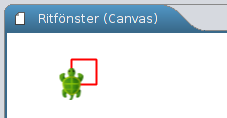
\includegraphics[width=0.47\textwidth]{../img/kojo/kvadrat}

\noindent Prova gärna olika sätt att skriva din kod \emph{utan} att resultatet ändras: skriv satser i sekvens på flera rader eller satser i sekvens på samma rad med semikolon emellan; använd blanktecken och blanka rader i koden. Hur vill du gruppera dina satser så att de är lätta för en människa att läsa?
%Prova att ändra på \emph{ordningen} mellan satserna och studera hur resultatet påverkas. Använd den \emph{gula} play-knappen  (programspårning) för att studera exekveringen i detalj. Vad händer du klickar på satser i ditt program och på rutor i programspårningen?


\Subtask Rita en trappa enligt bilden nedan.

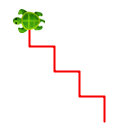
\includegraphics[width=0.3\textwidth]{../img/kojo/stairs}

\Subtask Rita valfri bild på valfri bakgrund med hjälp av några av procedurerna i tabellen nedan. Du kan till exempel rita en rosa triangel med lila konturer mot svart bakgrund. % \ref{lab:kojo:kojo-procedures}.
Försök att underlätta läsbarheten av din kod med hjälp av lämpliga radbrytningar och gruppering av satser.


\begin{table}[H]
\begin{longtable}{l l}\small
\code|fram(100)| & Paddan går framåt 100 steg (25 om argument saknas).\\
\code|färg(rosa)| & Sätter pennans färg till rosa. \\
\code|fyll(lila)| & Sätter ifyllnadsfärgen till lila. \\
\code|fyll(genomskinlig)| & Gör så att paddan \emph{inte} fyller i något när den ritar. \\
\code|bredd(20)| & Gör så att pennan får bredden 20. \\
\code|bakgrund(svart)| & Bakgrundsfärgen blir svart. \\
\code|bakgrund2(grön,gul)| & Bakgrund med övergång från grönt till gult. \\
\code|pennaNer|  & Sätter ner paddans penna så att den ritar när den går. \\
\code|pennaUpp|  & Sänker paddans penna så att den \emph{inte} ritar när den går. \\
\code|höger(45)|   & Paddan vrider sig 45 grader åt höger. \\
\code|vänster(45)| & Paddan vrider sig 45 grader åt vänster. \\
\code|hoppa|       & Paddan hoppar 25 steg utan att rita. \\
\code|hoppa(100)|  & Paddan hoppar 100 steg utan att rita. \\
\code|hoppaTill(100, 200)| & Paddan hoppar till läget (100, 200) utan att rita. \\
\code|gåTill(100, 200)|    & Paddan vrider sig och går till läget (100, 200). \\
\code|öster|   & Paddan vrider sig så att nosen pekar åt höger. \\
\code|väster|  & Paddan vrider sig så att nosen pekar åt vänster. \\
\code|norr|    & Paddan vrider sig så att nosen pekar uppåt. \\
\code|söder|   & Paddan vrider sig så att nosen pekar neråt. \\
\code|mot(100,200)|   & Paddan vrider sig så att nosen pekar mot läget (100, 200) \\
\code|sättVinkel(90)| & Paddan vrider nosen till vinkeln 90 grader. \\
\end{longtable}
%\label{lab:kojo:kojo-procedures}
%\caption{Några användbara procedurer i Kojo.}
\end{table}

\begin{framed}
\noindent\emph{Tips inför fortsättningen:} Ha gärna både REPL och Kojo igång samtidigt. Då kan du undersöka hur olika kodkonstruktioner fungerar i REPL, medan du stegvis skapar allt större program i editorn i Kojo. Detta sätt att jobba har du nytta av under resten av kursen, både om du använder en texteditor och kompilerar i terminalen, och om du använder en professionell integrerad utvecklingsmiljö. Oavsett vilka andra verktyg du kör är det användbart att ha REPL igång i ett eget fönster som hjälp i den kreativa processen, medan du jagar buggar och medan du lär dig nya koncept. Så fort du undrar hur något fungerar i Scala: fram med REPL och testa!
\end{framed}


\SOLUTION

\TaskSolved \what

\SubtaskSolved Genom att börja din Kojo-program med \code{sudda} så startar du exekveringen i samma utgångsläge: en tom rityta \Eng{canvas} där paddan pekar uppåt, pennan är nere och pennans färg är röd.  Då blir det lättare att resonera om vad programmet gör från början till slut, jämfört med om exekveringen beror på resultatet av tidigare exekveringar.


\SubtaskSolved
\begin{Code}
sudda

fram; vänster
fram; vänster
fram; vänster
fram; vänster
\end{Code}


\SubtaskSolved
\begin{Code}
sudda

fram; vänster
fram; höger

fram; vänster
fram; höger

fram; vänster
fram; höger

fram; vänster
\end{Code}


\QUESTEND









\clearpage

\ExtraTasks %%%%%%%%%%%%%%%%%% EXTRAUPPGIFTER



\WHAT{Typ och värde.}

\QUESTBEGIN

\Task \what~Vilket värde och vilken typ hör till vilket uttryck?  Är du osäker på svaret, testa i REPL.

\begin{ConceptConnections}[0.3\textwidth]
  \code|1.0 + 18          | & 1 & & A & \code|42.0: Double    | \\ 
  \code|(41 + 1).toDouble | & 2 & & B & \code|65: Int         | \\ 
  \code|1.042e42 + 1      | & 3 & & C & \code|19.0: Double    | \\ 
  \code|12E6.toLong       | & 4 & & D & \code|12000000: Long  | \\ 
  \code|32.toChar.toString| & 5 & & E & \code|'*': Char       | \\ 
  \code|'A'.toInt         | & 6 & & F & \code|48: Int         | \\ 
  \code|0.toInt           | & 7 & & G & \code|" ": String   | \\ 
  \code|'0'.toInt         | & 8 & & H & \code|1.042E42: Double| \\ 
  \code|'9'.toInt         | & 9 & & I & \code|'q': Char       | \\ 
  \code|'A' + '0'         | & 10 & & J & \code|113: Int        | \\ 
  \code|('A' + '0').toChar| & 11 & & K & \code|0: Int          | \\ 
  \code|"*!%#".charAt(0)| & 12 & & L & \code|57: Int         | \\ 
\end{ConceptConnections}

\SOLUTION

\TaskSolved \what

\begin{ConceptConnections}
  \code|1.0 + 18          | & 1 & ~~\Large$\leadsto$~~ &  E & \code|19.0: Double    | \\ 
  \code|(41 + 1).toDouble | & 2 & ~~\Large$\leadsto$~~ &  L & \code|42.0: Double    | \\ 
  \code|1.042e42 + 1      | & 3 & ~~\Large$\leadsto$~~ &  A & \code|1.042E42: Double| \\ 
  \code|12E6.toLong       | & 4 & ~~\Large$\leadsto$~~ &  K & \code|12000000: Long  | \\ 
  \code|32.toChar.toString| & 5 & ~~\Large$\leadsto$~~ &  G & \code|" ": String   | \\ 
  \code|'A'.toInt         | & 6 & ~~\Large$\leadsto$~~ &  H & \code|65: Int         | \\ 
  \code|0.toInt           | & 7 & ~~\Large$\leadsto$~~ &  I & \code|0: Int          | \\ 
  \code|'0'.toInt         | & 8 & ~~\Large$\leadsto$~~ &  F & \code|48: Int         | \\ 
  \code|'9'.toInt         | & 9 & ~~\Large$\leadsto$~~ &  D & \code|57: Int         | \\ 
  \code|'A' + '0'         | & 10 & ~~\Large$\leadsto$~~ &  B & \code|113: Int        | \\ 
  \code|('A' + '0').toChar| & 11 & ~~\Large$\leadsto$~~ &  J & \code|'q': Char       | \\ 
  \code|"*!%#".charAt(0)| & 12 & ~~\Large$\leadsto$~~ &  C & \code|'*': Char       | \\ 
\end{ConceptConnections}

%\Subtask \code{1.0 + 18}
%
%\Subtask \code{(41 + 1).toDouble}
%
%\Subtask \code{1.042e42 + 1}
%
%\Subtask \code{12E6.toLong}
%
%\Subtask \code{"gurk" + 'a'}
%
%\Subtask \code{32.toChar.toString}
%
%\Subtask \code{'A'.toInt}
%
%\Subtask \linebreak[0] \code{'0'.toInt}
%
%\Subtask \code{'0'.toInt}
%
%\Subtask \code{'9'.toInt}
%
%\Subtask \code{'A' + '0'}
%
%\Subtask \code{('A' + '0').toChar}
%
%\Subtask \code{"*!%#".charAt(0)}
%%%%%%%%%%%%%%%%%%%%%%%%%%%%%%%%%%%%%%%%%%%%%%%%
%\SubtaskSolved \code{Double, 19}
%
%\SubtaskSolved \code{Double, 42}
%
%\SubtaskSolved \code{Double, 1.042E42}
%
%\SubtaskSolved \code{Long, 12000000}
%
%\SubtaskSolved \code{String, gurka}
%
%\SubtaskSolved \code{String, " "}
%
%\SubtaskSolved \code{Int, 65}
%
%\SubtaskSolved \code{Int, 48}
%
%\SubtaskSolved \code{Int,49}
%
%\SubtaskSolved \code{Int,57}
%
%\SubtaskSolved \code{Int, 113}
%
%\SubtaskSolved \code{Char, 'q'}
%
%\SubtaskSolved \code{Char, '*'}


\QUESTEND




\WHAT{Satser och uttryck.}

\QUESTBEGIN

\Task \what

\Subtask Vad är det för skillnad på en sats och ett uttryck?

\Subtask Ge exempel på satser som inte är uttryck?

\Subtask Förklara vad som händer för varje evaluerad rad:
\begin{REPL}
scala> def värdeSaknas = ()
scala> värdeSaknas
scala> värdeSaknas.toString
scala> println(värdeSaknas)
scala> println(println("hej"))
\end{REPL}

\Subtask Vilken typ har literalen \code{()}?

\Subtask Vilken returtyp har \code{println}?

\SOLUTION

\TaskSolved \what

\SubtaskSolved  Ett utryck kan evalueras och resulterar då i ett användbart värde. En sats \emph{gör} något (t.ex. skriver ut något), men resulterat inte i något användbart värde.

\SubtaskSolved \code{println()}

\SubtaskSolved

 \code{värdeSaknas} innehåller Unit

 Skriver ut \code{Unit}

 Skriver ut \code{"()"}

 Skriver ut \code{"()"}

 Skriver först ut hej med det innersta anropet och sen \code{()} med det yttre anropet

\SubtaskSolved  \code{Unit}

\SubtaskSolved  \code{Unit}

\QUESTEND



\WHAT{Procedur med parameter.}

\QUESTBEGIN

\Task \what~En procedur är en funktion som orsakar en effekt, till exempel en utskrift eller en variabeltilldelning, men som inte returnerar något intressant resultatvärde.%
\footnote{I Scala är procedurer funktioner som returnerar det \emph{tomma värdet}, vilket skrivs \code{()} och är av typen \code{Unit}. I Java och flera andra språk finns inget tomt värde och man har en specialsyntax för procedurer som använder nyckelordet \code{void}. }

\Subtask Deklarera en förändringsbar variabel \code{highscore} som initieras till 0.

\Subtask Deklarera en procedur \code{updateHighscore} som tar en parameter \code{points} och tilldelar \code{highscore} ett nytt värde om \code{points} är större än \code{highscore} och skriver ut strängen \code{"REKORD!"}. Om inte \code{points} är större än \code{highscore} ska strängen \code{"GE INTE UPP!"} skrivas ut. Testa proceduren i REPL.

\Subtask Gör en ny variant av \code{updateHighscore}, som \emph{inte} är en procedur utan i stället är en funktion som ger en sträng för senare utskrift. Testa funktionen i REPL.

\SOLUTION

\TaskSolved \what

\SubtaskSolved
\begin{Code}
var highscore = 0
\end{Code}

\SubtaskSolved
\begin{Code}
def updateHighscore(points: Int): Unit =
  if points > highscore then
    highscore = points
    println("REKORD!")
  else println("GE INTE UPP!")
\end{Code}

\SubtaskSolved
\begin{Code}
def updateHighscore(points: Int): String =
  if points > highscore then
    highscore = points
    "REKORD!"
  else "GE INTE UPP!"
\end{Code}



\QUESTEND


\WHAT{Flyttalsaritmetik.}

\QUESTBEGIN

\Task \what

\Subtask Vilket är det minsta positiva värdet av typen \code{Double}?

\Subtask Vad är värdet av detta uttryck? Varför blir det så?
\begin{REPL}
scala> Double.MaxValue + Double.MinPositiveValue == Double.MaxValue
\end{REPL}

\SOLUTION

\TaskSolved \what

\SubtaskSolved

\begin{REPL}
scala> Double.MinPositiveValue
res0: Double = 4.9E-324
\end{REPL}

\SubtaskSolved

\begin{REPL}
scala> Double.MaxValue + Double.MinPositiveValue == Double.MaxValue
res2: Boolean = true
\end{REPL}

\QUESTEND



\WHAT{\code{if}\textit{-sats}.}

\QUESTBEGIN

\Task \what~För varje rad nedan, beskriv vad som skrivs ut.  % Uppgift 18
\begin{REPL}
scala> if !true then println("sant") else println("falskt")
scala> if !false then println("sant") else println("falskt")
scala> def singlaSlant = if math.random() < 0.5 then "krona" else "klave"
scala> for i <- 1 to 5 do print(s"$i:$singlaSlant ")
\end{REPL}

\SOLUTION

\TaskSolved \what

\begin{enumerate}
\item Utskrift: \code{falskt}
\item Utskrift: \code{sant}
\item Inget skrivs ut, funktionen deklareras men körs ej.
\item Utskrift: \code{1:krona 2:klave 3:krona 4:krona 5:klave } eller liknande beroende på vilka slumptal \code{math.random()} ger.
\end{enumerate}

\QUESTEND




\WHAT{\code{if}\textit{-uttryck}.}

\QUESTBEGIN

\Task  Deklarera följande variabler med nedan initialvärden:

\begin{REPLnonum}
scala> var grönsak = "gurka"
scala> var frukt = "banan"
\end{REPLnonum}

Ange för varje rad nedan vad uttrycket har för värde och typ:
\begin{REPLnonum}
scala> if grönsak == "tomat" then "gott" else "inte gott"
scala> if frukt == "banan" then "gott" else "inte gott"
scala> if true then grönsak else 42
scala> if false then grönsak else 42
\end{REPLnonum}

\SOLUTION


\TaskSolved \what~Notera typen \code{Any} på de sista två uttrycken.

\begin{REPLnonum}
scala> if grönsak == "tomat" then "gott" else "inte gott"
res0: String = inte gott

scala> if frukt == "banan" then "gott" else "inte gott"
res1: String = gott

scala> if true then grönsak else 42
res2: Any = gurka

scala> if false then grönsak else 42
res3: Any = 42
\end{REPLnonum}


\QUESTEND





\WHAT{Modulo-operatorn {\tt \%} och Booleska värden.}

\QUESTBEGIN

\Task \what

\Subtask Deklarera en funktion \code{def isEven(n: Int): Boolean = ???} som ger \code{true} om talet \code{n} är jämnt, annars \code{false}.

\Subtask Deklarera en funktion \code{def isOdd(n: Int): Boolean = ???} som ger \code{false} om talet \code{n} är jämnt, annars \code{true}.

\SOLUTION


\TaskSolved \what

\SubtaskSolved
\begin{REPL}
scala> def isEven(n: Int): Boolean = n % 2 == 0

scala> isEven(42)
res0: Boolean = true

scala> isEven(43)
res1: Boolean = false

\end{REPL}


\SubtaskSolved
\begin{REPL}
scala> def isOdd(n: Int): Boolean = !isEven(n)

scala> isOdd(42)
res2: Boolean = false

scala> isOdd(43)
res3: Boolean = true
\end{REPL}


\QUESTEND





\WHAT{Skillnader mellan \code{var}, \code{val}, \code{def}.}

\QUESTBEGIN

\Task \what~

\Subtask
 Evaluera varje rad en i taget i tur och ordning i Scala REPL. För varje rad nedan: förklara för vad som händer och notera värde och ev fel. % Uppgift 15
\begin{REPL}
scala> var x = 30
scala> x + 1
scala> x = x + 1
scala> x == x + 1
scala> val y = 20
scala> y = y + 1
scala> var z = { println("hej z!"); math.random() }
scala> def w = { println("hej w!"); math.random() }
scala> z
scala> z
scala> z = z + 1
scala> w
scala> w
scala> w = w + 1
\end{REPL}


\Subtask Vad är det för skillnad på \code{var}, \code{val} och \code{def}?



\SOLUTION

\TaskSolved \what

\SubtaskSolved
\begin{REPL}
  scala> var x = 30
  x: Int = 30

  scala> x + 1
  res6: Int = 31

  scala> x = x + 1
  x: Int = 31

  scala> x == x + 1
  res7: Boolean = false

  scala> val y = 20
  y: Int = 20

  scala> y = y + 1
  <console>:12: error: reassignment to val
         y = y + 1
           ^

  scala> var z = { println("hej z!"); math.random() }
  hej z!
  z: Double = 0.3381365875903367

  scala> def w = { println("hej w!"); math.random() }
  w: Double

  scala> z
  res8: Double = 0.3381365875903367

  scala> z
  res9: Double = 0.3381365875903367

  scala> z = z + 1
  z: Double = 1.3381365875903368

  scala> w
  hej w!
  res10: Double = 0.06420209879434557

  scala> w
  hej w!
  res11: Double = 0.5777951341051852

  scala> w = w + 1
  <console>:12: error: value w_= is not a member of object
         w = w + 1
\end{REPL}


\SubtaskSolved
\begin{itemize}
\item \code{var namn = uttryck} används för att deklarera en förändringsbar variabel. Namnet kan med hjälp av en tilldelningssats referera till nya värden.

\item \code{val namn = uttryck} används för att deklarera en oföränderlig variabel som efter initialisering inte kan förändras med tilldelningssatser. Vid försök ges kompileringsfel.
\item \code{def namn = uttryck} används för att deklarera en funktion vars uttryck evalueras varje gång den anropas.
\end{itemize}

\QUESTEND




\WHAT{Skillnaden mellan \code{if} och \code{while}.}

\QUESTBEGIN

\Task \what~Vad blir resultatet av rad 3 och 4?

\begin{REPL}
scala> def lotto1 = if math.random() > 0.5 then print("vinst :) ")
scala> def lotto2 = while math.random() > 0.5 do print("vinst :) ")
scala> lotto1
scala> lotto2
\end{REPL}

\SOLUTION

\TaskSolved \what

\begin{itemize}
\item Rad 3: Har du tur (50\% chans) får du vinst en gång.

\item Rad 4: Har du tur får du många vinster i rad. Sannolikheten för $n$ vinster i rad är $(\frac{1}{2})^n$.
\end{itemize}
\QUESTEND












\clearpage

\AdvancedTasks   %%%%%%%%%%%%%%%%%%% FÖRDJUPNINGSUPPGIFTER





\WHAT{Logik och De Morgans Lagar.}

\QUESTBEGIN

\Task \what~Förenkla följande uttryck. Antag att \code{poäng} och \code{highscore} är heltalsvariabler medan \code{klar} är av typen \code{Boolean}.
  % Uppgift 24

\Subtask \code{poäng > 100 && poäng > 1000}

\Subtask \code{poäng > 100 || poäng > 1000}

\Subtask \code{!(poäng > highscore)}

\Subtask \code{!(poäng > 0 && poäng < highscore) }

\Subtask \code{!(poäng < 0 || poäng > highscore) }

\Subtask \code{klar == true}

\Subtask \code{klar == false}

\SOLUTION

\TaskSolved \what


\SubtaskSolved \code{poäng > 1000}

\SubtaskSolved \code{poäng > 100}

\SubtaskSolved \code{poäng <= highscore}

\SubtaskSolved \code{poäng <= 0 || poäng >= highscore }

\SubtaskSolved \code{poäng >= 0 && poäng <= highscore}

\SubtaskSolved \code{klar}

\SubtaskSolved \code{!klar}


\QUESTEND






\WHAT{Stränginterpolatorn \code{s}.}

\QUESTBEGIN

\Task \what~Med ett \code{s} framför en strängliteral får man hjälp av kompilatorn att, på ett typsäkert sätt, infoga variabelvärden i en sträng.
Variablernas namn ska föregås med ett dollartecken , t.ex. \code{s"Hej $namn"}.
Om man vill evaluera ett uttryck placeras detta inom klammer direkt efter dollartecknet, t.ex.
\code/s"Dubbla längden: ${namn.size * 2}"/

\Subtask Vad skrivs ut nedan?
\begin{REPL}
scala> val f = "Kim"
scala> val e = "Finkodare"
scala> println(s"Namnet '$f $e' har ${f.size + e.size} bokstäver.")
\end{REPL}

\Subtask Skapa följande utskrifter med hjälp av stränginterpolatorn \code{s} och variablerna \code{f} och \code{e} i föregående deluppgift.
\begin{REPL}
Kim har 3 bokstäver.
Finkodare har 9 bokstäver.
\end{REPL}

\SOLUTION

\TaskSolved \what

\SubtaskSolved
\begin{REPLnonum}
Namnet 'Kim Finkodare' har 12 bokstäver.
\end{REPLnonum}

\SubtaskSolved
\begin{REPLnonum}
println(s"$f har  ${f.size} bokstäver.")
println(s"$e har  ${e.size} bokstäver.")
\end{REPLnonum}

\QUESTEND



\WHAT{Tilldelningsoperatorer.}

\QUESTBEGIN

\Task \what~Man kan förkorta en tilldelningssats som förändrar en variabel, t.ex. \code{x = x + 1}, genom att använda så kallade tilldelningsoperatorer och skriva \code{x += 1} som betyder samma sak. Rita en ny bild av datorns minne efter varje rad nedan. Bilderna ska visa variablers namn, typ och värde.

\begin{REPL}
scala> var a = 40
scala> var b = a + 40
scala> a += 10
scala> b -= 10
scala> a *= 2
scala> b /= 2
\end{REPL}

\SOLUTION

\TaskSolved \what

\begin{tabular}{l l}
\MEM{{\it Efter rad1:~~~~} a}{Int}{40}\\
\MEM{{\it Efter rad2:~~~~} a}{Int}{40} & \MEM{b}{Int}{80}\\
\MEM{{\it Efter rad3:~~~~} a}{Int}{50} & \MEM{b}{Int}{80}\\
\MEM{{\it Efter rad4:~~~~} a}{Int}{50} & \MEM{b}{Int}{70} \\
\MEM{{\it Efter rad5:~~~~} a}{Int}{100} & \MEM{b}{Int}{70} \\
\MEM{{\it Efter rad6:~~~~} a}{Int}{100} & \MEM{b}{Int}{35} \\
\end{tabular}

\QUESTEND






\WHAT{Stora tal.}

\QUESTBEGIN

\Task \what~Om vi vill beräkna $2^{64} -1$ som ett exakt heltal\footnote{\url{https://en.wikipedia.org/wiki/Wheat_and_chessboard_problem}} blir det större än \code{Int.MaxValue}, så vi kan tyvärr inte använda snabba \code{Int}. Till vår räddning: \code{BigInt}

\Subtask Läs om \code{BigInt} och \code{BigDecimal} på \Scaladoc \\ Notera vad de kan användas till.

\Subtask Du skapar ett \code{BigInt}-heltal med \code{BigInt(2)} och kan anropa funktionen \code{pow} på en \code{BigInt} med punktnotation. Beräkna $2^{64} -1$ som ett exakt heltal.

\Subtask Vilka nackdelar finns med \code{BigInt} och \code{BigDecimal}?

\SOLUTION

\TaskSolved \what

\SubtaskSolved \code{BigInt} kan användas i stället för \code{Int} vid mycket stora heltal. Det finns förståss även \code{Long} som har dubbelt omfång jämfört med \code{Int}, medan \code{BigInt} kan ha godtyckligt många siffror (ända tills minnet tar slut) och kan därmed representera ofantligt stora tal. \code{BigDecimal} kan användas i stället för \code{Double} vid mycket stora decimaltal.

\SubtaskSolved
\begin{REPL}
scala> BigInt(2).pow(64)
res0: scala.math.BigInt = 18446744073709551616
\end{REPL}

\SubtaskSolved Beräkningar går mycket långsammare och de är lite krångligare att använda.

\QUESTEND





\WHAT{Precedensregler}

\QUESTBEGIN

\Task \what~Evalueringsordningen kan styras med parenteser. Vilket värde och vilken typ har följande uttryck?

\Subtask \code{23 + 2 * 2 + (23 + 2) * 2}

\Subtask \code{(-(2 - 42)) / (1 + 1 + 1)}

\Subtask \code{(-(2 - 42)) / (-1)/(1 + 1 + 1)}

\SOLUTION

\TaskSolved \what

\SubtaskSolved \code{77:  Int}

\SubtaskSolved \code{13: Int}

\SubtaskSolved \code{-13: Int}

\QUESTEND



\WHAT{Dokumentation av paket i Java och Scala.}

\QUESTBEGIN

\Task \what


\Subtask Genom att trycka på tab tangenten kan man se vad som finns i olika paket. Vad heter konstanten $\pi$  i \code{java.lang.Math} (notera stort M) respektive \code{scala.math.}?

\begin{REPL}
scala> java.lang.Math.    //tryck TAB efter punkten
scala> scala.math.        //tryck TAB efter punkten
\end{REPL}

\Subtask Jämför dokumentationen för klassen \code{java.lang.Math} här: \\ \url{https://docs.oracle.com/javase/8/docs/api/} \\
med dokumentationen för paketet \code{scala.math} här: \\
\url{http://www.scala-lang.org/api} \\
Ge exempel på vad man kan göra på webbsidan med Scala-dokumentationen som man \emph{inte} kan göra i motsvarande webbsida Java-dokumentation.

\Subtask Vad gör metoden \code{hypot}? Vad är det som är bra med att använda \code{hypot} i stället för att själv implementera beräkningen med hjälp av kvadratrot, multiplikation och addition?

\SOLUTION

\TaskSolved \what

\SubtaskSolved Scala: \code{Pi}, Java: \code{PI}

\SubtaskSolved Man kan söka och filtrera fram alla förekomster av en viss teckenkombination.

\SubtaskSolved Räknar ut hypotenusan (Pythagoras sats) utan risk för avrundningsproblem i mellanberäkningar.


\QUESTEND





\WHAT{Noggrannhet och undantag i aritmetiska uttryck.}

\QUESTBEGIN

\Task \what~Vad blir resultatet av uttrycken nedan? Notera undantag \Eng{exceptions} och noggrannhetsproblem.

\Subtask \code{Int.MaxValue + 1}

\Subtask \code{1 / 0}

\Subtask \code{1E8 + 1E-8}

\Subtask \code{1E9 + 1E-9}

\Subtask \code{math.pow(math.hypot(3,6), 2)}

\Subtask\Uberkurs \code{1.0 / 0}

\Subtask\Uberkurs \code{(1.0 / 0).toInt}

\Subtask\Uberkurs \code{math.sqrt(-1)}

\Subtask\Uberkurs \code{math.sqrt(Double.NaN)}

\Subtask \code{throw new Exception("PANG!!!")}

\SOLUTION

\TaskSolved \what

\SubtaskSolved \code{-2147483648} vilket motsvarar \code{Int.MinValue}.

\SubtaskSolved Ett undantag kastas: \code{java.lang.ArithmeticException: / by zero}

\SubtaskSolved \code{1.0000000000000001E8} (som förväntat)

\SubtaskSolved Avrundas till \code{1E9} (flyttalsaritmetik med noggrannhetsproblem: ett stort flyttal plus ett (alltför) litet flyttal kan ge samma tal. Det lilla talet ''försvinner'').


\SubtaskSolved \code{45.00000000000001} (flyttalsaritmetik med noggrannhetsproblem: enligt ''normal'' aritmetik ska det bli exakt 45.)

\SubtaskSolved \code{Infinity} (som även ges av \code{Double.PositiveInfinity} och som representerar den positiva oändligheten).

\SubtaskSolved \code{2147483647} vilket motsvarar \code{Int.MaxValue}.

\SubtaskSolved \code{NaN} vilket betyder ''Not a Number''.

\SubtaskSolved \code{NaN} vilket betyder ''Not a Number''.

\SubtaskSolved Ett undantag kastas: \code{java.lang.Exception: PANG!!!}

\QUESTEND



\WHAT{Modulo-räkning med negativa tal.}

\QUESTBEGIN

\Task\Uberkurs \what~Läs om moduloräkning här: \\
 \href{https://en.wikipedia.org/wiki/Modulo\_operation}{en.wikipedia.org/wiki/Modulo\_operation} \\
 och undersök hur det blir med olika tecken (positivt resp. negativt) på moduloräkning med $dividend \% divisor$ i Scala.


\SOLUTION

\TaskSolved \what~I Scala har resultatet samma tecken som dividenden.
\begin{REPL}
scala> 1 % 2
res0: Int = 1

scala> -1 % 2
res1: Int = -1

scala> -1 % -2
res2: Int = -1

scala> 1 % -2
res3: Int = 1

\end{REPL}

\QUESTEND




\WHAT{Bokstavliga identifierare.}

\QUESTBEGIN

\Task\Uberkurs \what~Läs om identifierare i Scala och speciellt \emph{literal identifiers} här: \url{http://www.artima.com/pins1ed/functional-objects.html#6.10}.

\Subtask Förklara vad som händer nedan:
\begin{REPLnonum}
scala> val `bokstavlig val` = 42
scala> println(`bokstavlig val`)
\end{REPLnonum}

\Subtask Scala och Java har olika uppsättningar med reserverade ord. På vilket sätt kan ''backticks'' vara använbart med anledning av detta?

\SOLUTION

\TaskSolved \what

\SubtaskSolved Variabeln får namnet 'bokstavlig val', bakåt-apostrofer \Eng{backticks} gör att man kan namnge variabler till annars otillåtna namn, t.ex. med mellanrum eller nyckelord i sig.

\SubtaskSolved Backticks i Scala möjliggör alla möjliga tecken i namn. Exempel på användning: I java finns en metod som heter \jcode{java.lang.Thread.yield} men i Scala är yield ett nyckelord; för att komma runt det går det att i Scala skriva \jcode{java.lang.Thread.`yield`}

\QUESTEND












\WHAT{\code{java.lang.Integer}, hexadecimala litteraler, BigDecimal.}

\QUESTBEGIN

\Task\Uberkurs \what~

\Subtask Sök upp dokumentationen för \code{java.lang.Integer}.\\Använd metoderna \code{toBinaryString} och \code{toHexString} för att fylla i tabellen nedan.

\begin{table}[H]
\begin{tabular}{l | l | l}
decimalt heltal & binärt värde & hexadecimalt värde \\
\hline
$33$ &   &  \\
$42$ &   &  \\
$64$ &   &  \\
\end{tabular}
\end{table}

\Subtask Hur anger man det hexadecimala heltalsvärdet 10c (motsvarar 268 decimalt) som en litteral i Scala?

\Subtask Vad blir \code{0x10} upphöjt till $c =$ ljusets hastighet i $m/s$? \emph{Tips:} Använd \code{BigDecimal}.

\SOLUTION

\TaskSolved \what

\SubtaskSolved

\begin{REPL}
scala> import Integer.{toBinaryString => toBin, toHexString => toHex}

scala> for i <- Seq(33, 42, 64) do println(s"$i \t ${toBin(i)} \t ${toHex(i)}")
33 	 100001 	 21
42 	 101010 	 2a
64 	 1000000 	 40
\end{REPL}


\SubtaskSolved Det hexadecimala heltalet $10c$ kan anges med litteralen \code{0x10c} i Scala, Java och många andra språk: \footnote{\url{https://en.wikipedia.org/wiki/0x10c}}
\begin{REPL}
scala> 0x10c
res0: Int = 268
\end{REPL}

\SubtaskSolved \footnote{\url{https://c418.bandcamp.com/album/0x10c}}
\begin{REPL}
scala> val c = 299792458
c: Int = 299792458

scala> BigDecimal(0x10).pow(c)
res68: scala.math.BigDecimal = 2.124892963227906613060986110887672E+360986089
\end{REPL}


\QUESTEND









\WHAT{Strängformatering.}

\QUESTBEGIN

\Task\Uberkurs \what~Läs om \code{f}-interpolatorn här:\\
\url{http://docs.scala-lang.org/overviews/core/string-interpolation.html} \\
Hur kan du använda \code{f}-interpolatorn för att göra följande utskrift i REPL? Ändra rad 3 vid \code{???} så att flyttalet \code{g} avrundas till tre decimaler innan utskrift sker.
\begin{REPL}
scala> val g = 2 / 3.0
scala> val str = f"Jättegurkan är $g??? meter lång"
scala> println(str)
Jättegurkan är 0.667 meter lång
\end{REPL}

\SOLUTION

\TaskSolved \what

\begin{Code}
val str = f"Jättegurkan är $g%1.3f meter lång"
\end{Code}
(Om du tycker att \code{$g%1.3f}
ser kryptiskt ut, så kan du trösta dig med att du nu får chansen att föra vidare ett anrikt arv från det urgamla språket C och den sägenomspunna funktionen \code{printf} till kommande generationer av invigda kodmagiker.)

\QUESTEND




\WHAT{Multiplikationsvarning.}

\QUESTBEGIN

\Task \what~Sök upp dokumentationtionen för\\\code{java.lang.Math.multiplyExact} och läs om vad den metoden gör.

\Subtask Vad händer här?

\begin{REPLnonum}
scala> Math.multiplyExact(1, 2)
scala> Int.MaxValue * 2
scala> Math.multiplyExact(Int.MaxValue, 2)
\end{REPLnonum}

\Subtask Varför kan man vilja använda \code{java.lang.Math.multiplyExact} i stället för ''vanlig'' multiplikation?

\SOLUTION

\TaskSolved \what

\SubtaskSolved Den andra multiplikationen flödar över \Eng{overflow} gränsen för största möjliga värdet av en \code{Int}. I den tredje multiplikationen kastas i stället ett undantag \code{java.lang.ArithmeticException: integer overflow}


\begin{REPLnonum}
scala> Math.multiplyExact(1, 2)
res70: Int = 2

scala> Int.MaxValue * 2
res71: Int = -2

scala> Math.multiplyExact(Int.MaxValue, 2)
java.lang.ArithmeticException: integer overflow
  at java.lang.Math.multiplyExact(Math.java:867)
  ... 42 elided
\end{REPLnonum}

\SubtaskSolved Används då man vill vara helt säker på att overflow-buggar ''smäller'' direkt i stället för att generera felaktiga resultat vars konsekvenser kanske manifesterar sig långt senare. Dock är \code{multiplyExact} aningen långsammare än vanlig multiplikation.


\QUESTEND








\WHAT{Dekorera \code{Int} med extra operatorer.}

\QUESTBEGIN

\Task\Uberkurs \what\footnote{En utmanande överkursuppgift som visar Scalas kraftfullhet. Se fördjupningslänkar i facit.}\\Kim Kodmagiker tycker att \code{Math.multiplyExact} är för krångligt att skriva och utökar därför typen \code{Int} med en extra operator:

\begin{Code}
implicit class IntDecorator(val i: Int) extends AnyVal {
  def *!(j: Int) = Math.multiplyExact(i,j)
}
\end{Code}

\Subtask Klistra in koden ovan i REPL och prova den extra operatorn.

\Subtask Hjälp Kim Kodmagiker att lägga till fler operatorer på värden av typen \code{Int}, som gör att det även går att använda \code{Math.subtractExact} och \code{Math.addExact} smidigt.

\Subtask Testa ett sammansatt uttryck som använder alla extrametoder på \code{Int}. Tycker du det blev mer lättläst eller mer kryptiskt med de nya operatorerna?

\SOLUTION

\TaskSolved \what

\SubtaskSolved

\begin{REPL}
scala> Int.MaxValue *! 1
res0: Int = 2147483647

scala> Int.MaxValue *! 2
java.lang.ArithmeticException: integer overflow
  at java.lang.Math.multiplyExact(Math.java:867)
  at IntExtra.$times$bang(<console>:16)
  ... 32 elided

\end{REPL}

Kort förklaring:
\begin{itemize}
\item \code{implicit class MinDekorator(x: Typ)} gör så att operationer i dekoratorklassen \code{MinDekorator} automatiskt görs tillgängliga på värden av typen \code{Typ}.%
\footnote{Fördjupning: \url{http://docs.scala-lang.org/overviews/core/implicit-classes.html}}

\item \code{extends AnyVal} gör så att kompilatorn försöker generera maskinkod som blir lika effektiv som vid direkt användning av det underliggande värdet.%
\footnote{Fördjupning: \url{http://docs.scala-lang.org/overviews/core/value-classes.html}}
\end{itemize}


\SubtaskSolved

\begin{Code}
implicit class IntDecorator(val i: Int) extends AnyVal{
  def *!(j: Int) = Math.multiplyExact(i,j)
  def +!(j: Int) = Math.addExact(i,j)
  def -!(j: Int) = Math.subtractExact(i,j)
}
\end{Code}


\SubtaskSolved Det blir lätt väldigt kryptiskt med namn som består av flera specialtecken. Om du \emph{verkligen} vill ha sådana operatorer är det \emph{mycket} lämpligt att också erbjuda varianter i klartext:
\begin{Code}
implicit class IntDecorator(val i: Int) extends AnyVal{
  def mulExact(j: Int) = Math.multiplyExact(i,j)
  def *!(j: Int) = i mulExact j

  def addExact(j: Int) = Math.addExact(i,j)
  def +!(j: Int) = i addExact j

  def subExact(j: Int) = Math.subtractExact(i,j)
  def -!(j: Int) = i subExact j
}

\end{Code}


\QUESTEND



%%%%%%%%%%%%%%%%%%%%%%%%%%%%%%%%%%%%%%%%%%%%%%%%
%%%%%%%%%%%%%%%%%%%%%%%%%%%%%%%%%%%%%%%%%%%%%%%%
%%%%%%%%%%%%%%%%%%%%%%%%%%%%%%%%%%%%%%%%%%%%%%%%
%%%%%%%%%%%%%%%%%%%%%%%%%%%%%%%%%%%%%%%%%%%%%%%%
%%%%%%%%%%%%%%%%%%%%%%%%%%%%%%%%%%%%%%%%%%%%%%%%
%%%%%%%%%%%%%%%%%%%%%%%%%%%%%%%%%%%%%%%%%%%%%%%%
%%%%%%%%%%%%%%%%%%%%%%%%%%%%%%%%%%%%%%%%%%%%%%%%
%%%%%%%%%%%%%%%%%%%%%%%%%%%%%%%%%%%%%%%%%%%%%%%%
%%%%%%%%%%%%%%%%%%%%%%%%%%%%%%%%%%%%%%%%%%%%%%%%


%% Saker som inte fick plats:



%\Task Läs om BigInt och BigDecimal här: \href{http://alvinalexander.com/scala/how-to-use-large-integer-decimal-numbers-in-scala-bigint-bigdecimal}{alvinalexander.com/scala/how-to-use-large-integer-decimal-numbers-in-scala-bigint-bigdecimal} och prova att skapa riktigt stora tal med hjälp av metoden \code{pow} på BigInt och tal med riktigt många decimaler med BigDecimal dess metod \code{pow}.


%
%
%\Subtask\Pen Sök med Ctrl+F i webbläsaren och efter förekomster av texten \textit{''overflow''} i javadoc för klassen \code{java.lang.Math} i JDK 8. Vad är ''overflow''? Vilka metoder finns i \code{java.lang.Math} som hjälper dig att upptäcka om det blir overflow?
%
%\Task Använda Scala REPL för att undersöka konstanterna nedan. Vilket av dessa värden är negativt? Vad kan man ha för praktisk nytta av dessa värden i ett program som gör flyttalsberäkningar?
%
%\Subtask \code{java.lang.Double.MIN_VALUE}
%
%\Subtask \code{scala.Double.MinValue}
%
%\Subtask \code{scala.Double.MinPositiveValue}
%
%\Task För typerna \code{Byte}, \code{Short}, \code{Char}, \code{Int}, \code{Long}, \code{Float}, \code{Double}: Undersök hur många bitar som behövs för att representera varje typs omfång? \\*
%\textit{Tips:} Några användbara uttryck: \\*
% \code{Integer.toBinaryString(Int.MaxValue + 1).size} \\*
% \code{Integer.toBinaryString((math.pow(2,16) - 1).toInt).size} \\*
% \code{1 + math.log(Long.MaxValue)/math.log(2)}
%Se även språkspecifikationen för Scala, kapitlet om heltalsliteraler: \\
%\url{http://www.scala-lang.org/files/archive/spec/2.11/01-lexical-syntax.html#integer-literals}
%
%\Subtask Undersök källkoden för paketobjektet \code{scala.math} här: \\
%\url{https://github.com/scala/scala/blob/v2.11.7/src/library/scala/math/package.scala} \\
%Hur många olika överlagrade varianter av funktionen \code{abs} finns det och för vilka parametertyper är den definierad?


%!TEX encoding = UTF-8 Unicode
%!TEX root = ../exercises.tex

\ifPreSolution

\Exercise{\ExeWeekTWO}\label{exe:W02}
\begin{Goals}
%!TEX encoding = UTF-8 Unicode
%!TEX root = ../compendium2.tex

\item Kunna skapa samlingarna Range, Array och Vector med heltals- och strängvärden.
\item Kunna indexera i en indexerbar samling, t.ex. Array och Vector.
\item Kunna anropa operationerna size, mkString, sum, min, max på samlingar som innehåller heltal.
\item Känna till grundläggande skillnader och likheter mellan samlingarna Range, Array och Vector.
\item Förstå skillnaden mellan en for-sats och ett for-uttryck.
\item Kunna skapa samlingar med heltalsvärden som resultat av enkla for-uttryck.
\item Förstå skillnaden mellan en algoritm i pseudo-kod och dess implementation.
\item Kunna implementera algoritmerna SUM, MIN/MAX på en indexerbar samling med en \code{while}-sats.
\item Kunna köra igång enkel Scala-kod i REPL, som skript och som applikation.
\item Kunna skriva och köra igång ett enkelt Java-program.
\item Känna till några grundläggande syntaxskillnader mellan Scala och Java, speciellt variabeldeklarationer och indexering i Array.
\item Förstå vad ett block och en lokal variabel är.
\item Förstå hur nästlade block påverkar namnsynlighet och namnöverskuggning.
\item Förstå kopplingen mellan paketstruktur och kodfilstruktur.
\item Kunna skapa en jar-fil.
\item Kunna skapa dokumentation med scaladoc.

\end{Goals}

\begin{Preparations}
\item \StudyTheory{02}
\item Bekanta dig med grundläggande terminalkommandon, se appendix~\ref{appendix:terminal}.
\item Bekanta dig med den editor du vill använda, se appendix~\ref{appendix:compile}.
\end{Preparations}

\else

\ExerciseSolution{\ExeWeekTWO}

\fi


% TODO fundera på detta:
% terminalkommando
% scalac -> hello world; scala som script; javac
% paket, import, jar, main,



\BasicTasksNoLab %%%%%%%%%%%%%%%%




\WHAT{Para ihop begrepp med beskrivning.}

\QUESTBEGIN

\Task \what

\vspace{1em}\noindent Koppla varje begrepp med den (förenklade) beskrivning som passar bäst:

\begin{ConceptConnections}
  kompilerad & 1 & & A & datastruktur med element av samma typ \\ 
  skript & 2 & & B & en oföränderlig, indexerbar sekvenssamling \\ 
  objekt & 3 & & C & en specifik realisering av en algoritm \\ 
  main & 4 & & D & maskinkod sparas ej utan skapas vid varje körning \\ 
  programargument & 5 & & E & applicerar en funktion på varje element i en samling \\ 
  datastruktur & 6 & & F & datastruktur med element i en viss ordning \\ 
  samling & 7 & & G & där exekveringen av kompilerad app startar \\ 
  sekvenssamling & 8 & & H & maskinkod sparad och kan köras igen utan kompilering \\ 
  Array & 9 & & I & en förändringsbar, indexerbar sekvenssamling \\ 
  Vector & 10 & & J & stegvis beskrivning av en lösning på ett problem \\ 
  Range & 11 & & K & en samling som representerar ett intervall av heltal \\ 
  yield & 12 & & L & samlar variabler och funktioner \\ 
  map & 13 & & M & många olika element i en helhet; elementvis åtkomst \\ 
  algoritm & 14 & & N & överförs via parametern args i main \\ 
  implementation & 15 & & O & används i for-uttryck för att skapa ny samling \\ 
\end{ConceptConnections}

\SOLUTION

\TaskSolved \what

\begin{ConceptConnections}
  kompilerad & 1 & ~~\Large$\leadsto$~~ &  L & maskinkod sparad och kan köras igen utan kompilering \\ 
  skript & 2 & ~~\Large$\leadsto$~~ &  F & maskinkod sparas ej utan skapas vid varje körning \\ 
  objekt & 3 & ~~\Large$\leadsto$~~ &  N & samlar variabler och funktioner \\ 
  main & 4 & ~~\Large$\leadsto$~~ &  G & där exekveringen av kompilerad app startar \\ 
  programargument & 5 & ~~\Large$\leadsto$~~ &  I & överförs via parametern args i main \\ 
  datastruktur & 6 & ~~\Large$\leadsto$~~ &  E & många olika element i en helhet; elementvis åtkomst \\ 
  samling & 7 & ~~\Large$\leadsto$~~ &  O & datastruktur med element av samma typ \\ 
  sekvenssamling & 8 & ~~\Large$\leadsto$~~ &  K & datastruktur med element i en viss ordning \\ 
  Array & 9 & ~~\Large$\leadsto$~~ &  B & en förändringsbar, indexerbar sekvenssamling \\ 
  Vector & 10 & ~~\Large$\leadsto$~~ &  D & en oföränderlig, indexerbar sekvenssamling \\ 
  Range & 11 & ~~\Large$\leadsto$~~ &  J & en samling som representerar ett intervall av heltal \\ 
  yield & 12 & ~~\Large$\leadsto$~~ &  C & används i for-uttryck för att skapa ny samling \\ 
  map & 13 & ~~\Large$\leadsto$~~ &  A & applicerar en funktion på varje element i en samling \\ 
  algoritm & 14 & ~~\Large$\leadsto$~~ &  M & stegvis beskrivning av en lösning på ett problem \\ 
  implementation & 15 & ~~\Large$\leadsto$~~ &  H & en specifik realisering av en algoritm \\ 
\end{ConceptConnections}

\QUESTEND





\WHAT{Använda terminalen.}

\QUESTBEGIN

\Task \what~Läs om terminalen i appendix \ref{appendix:terminal}.

\Subtask Vilka tre kommando ska du köra för att 1) skapa en katalog med namnet \code{hello} och 2)  navigera till katalogen och 3) visa namnet på ut aktuell katalog? Öppna ett teminalfönster och kör dessa tre kommando.

\Subtask Vilka två kommando ska du köra för att 1) navigera tillbaka ''upp'' ett steg i filträdet och 2) lista alla filer och kataloger på denna plats? Kör dessa två kommando i terminalen.

\SOLUTION

\TaskSolved \what

\SubtaskSolved

\begin{REPL}
> mkdir hello
> cd hello
> pwd
\end{REPL}

\SubtaskSolved

\begin{REPL}
> cd ..
> ls
\end{REPL}


\QUESTEND









\WHAT{Skapa och köra ett Scala-skript.}

\QUESTBEGIN

\Task  \what~

\Subtask Skapa en fil med namn \texttt{sum.scala} i katalogen \code{hello} som du skapade i föregående uppgift med hjälp av en editor, t.ex. \code{atom}.
\begin{REPLnonum}
> cd hello
> atom sum.scala
\end{REPLnonum}

\noindent Filen ska innehålla dessa tre rader:
\scalainputlisting{examples/sum.scala}

\noindent Spara filen och kör kommandot \code{scala sum.scala} i terminalen:
\begin{REPLnonum}
> scala sum.scala
\end{REPLnonum}

\noindent Vad blir summan av de $1000$ första talen?

\Subtask Ändra i filen \code{sum.scala} så att högerparentesen på sista raden saknas. Spara filen (Ctrl+S) och kör skriptfilen igen i terminalen (pil-upp). Hur lyder felmeddelandet? Är det ett körtidsfel eller ett kompileringsfel?

\Subtask Ändra i hello-script.scala så att det i stället för \code{1000} står \code{args(0).toInt} efter \code{val n =} och spara och kör om ditt program med argumentet 5001 så här:
\begin{REPL}
> scala hello-script.scala 5001
\end{REPL}
\noindent Vad blir summan av de $5001$ första talen?

\Subtask Vad blir det för felmeddelande om du glömmer ge programmet ett argument? Är det ett körtidsfel eller ett kompileringsfel?

\SOLUTION

\TaskSolved \what

\SubtaskSolved
\begin{REPL}
Summan av de 1000 första talen är: 500500
\end{REPL}

\SubtaskSolved  Kompileringsfelet blir: \code{error: ')' expected but eof found}

\SubtaskSolved  Filen ska se ut så här:
\begin{Code}
val n = args(0).toInt
val summa = (1 to n).sum
println(s"Summan av de $n första talen är: $summa")
\end{Code}

Utskriften blir så här:
\begin{REPL}
Summan av de 5001 första talen är: 12507501
\end{REPL}

\SubtaskSolved Körtidsfelet blir: \code{java.lang.ArrayIndexOutOfBoundsException: 0}\\(Anledningen är att arrayen \code{args} blir tom om programargument saknas och platsen med index $0$ därmed inte finns.)

\QUESTEND





\WHAT{Scala-applikation med \code+main+-metod.}

\QUESTBEGIN

\Task  \what~  Skapa med hjälp av en editor en fil med namn \texttt{hello.scala}.
\begin{REPLnonum}
> atom hello.scala
\end{REPLnonum}
Skriv nedan kod i filen:


\scalainputlisting{examples/hello.scala}

\Subtask Kompilera med \code{scalac hello.scala} och kör koden med \code{scala Hello}. Notera stor bokstav i klassnamnet. Vad heter filerna som kompilatorn skapar?
\begin{REPLnonum}
> scalac hello.scala
> ls
> scala Hello
\end{REPLnonum}

\Subtask Hur ska du ändra i din kod så att kompilatorn ger följande felmeddelande: \\
\texttt{Missing closing brace}

\Subtask Varför behövs \code{main}-metoden?

\Subtask Vilket alternativ går snabbast att köra igång, ett skript eller en kompilerad applikation? Varför? Vilket alternativ kör snabbast när väl exekveringen är igång?


\SOLUTION


\TaskSolved \what


\SubtaskSolved  Filerna som kompilatorn skapat heter \code{Hello.class} och \verb+Hello\$.class+

\SubtaskSolved  Felmeddelandet får du om du tar bort den sista krullparentesen.

\SubtaskSolved

\begin{itemize}
  \item  Det går snabbare att göra i gång en kompilerad app eftersom maskinkoden är sparad i en fil som kan köras igång direkt. En kompilerad app måste ha ett objekt med en main-metod. En kompilerad app kan bestå av många filer som samkompileras.
  \item När ett skript kör kompileras koden i skriptfilen före varje körning och maskinkoden sparas inte. Ett skript består bara av en enda text-fil som körs från början. Ingen main-metod behövs.
  \item  När väl exekveringen är igång sker exekveringen av maskinkoden exakt lika snabbt oberoende av om koden är genererad ur ett skript eller en förkompilerad app.
\end{itemize}

\QUESTEND







\WHAT{Java-applikation.}

\QUESTBEGIN

\Task \label{task:java} \what~   Skapa med hjälp av en editor en fil med namn \texttt{Hi.java}. Notera stor bokstav. I ett Java-program måste namnet före \code{.java} stämma överens exakt med klassnamnet.
\begin{REPLnonum}
> atom Hi.java
\end{REPLnonum}
Skriv dessa rader i filen:
\javainputlisting{examples/Hi.java}
\noindent Kompilera med \code{javac Hi.java} och kör koden med \code{java Hi}.
\begin{REPLnonum}
> javac Hi.java
> ls
> java Hi
\end{REPLnonum}

\Subtask Vad heter filen som kompilatorn skapat?

\Subtask Jämför Java-programmet ovan med Scala-programmet i föregående uppgift. Programmen gör samma sak men syntaxen (hur koden ska skrivas) skiljer sig åt och det finns vissa skillnader i semantiken (vad koden betyder). Vi ska senare i kursen gå igenom \emph{exakt} vad varje fragment nedan betyder, men försök redan nu para ihop de Scala-delar till vänster som (ungefär) motsvarar de Java-delar som finns till höger.

\begin{ConceptConnections}
  \code|object| & 1 & & A & \jcode|public static main| \\ 
  \code|def main| & 2 & & B & \jcode|public class| \\ 
  \code|Array[String]| & 3 & & C & \jcode|void| \\ 
  \code|: Unit| & 4 & & D & \jcode|) {| \\ 
  \code|=| & 5 & & E & \jcode|System.out.println| \\ 
  \code|println| & 6 & & F & \jcode|String[]| \\ 
\end{ConceptConnections}

\SOLUTION


\TaskSolved \what


\SubtaskSolved  Hi.class

\SubtaskSolved

\begin{ConceptConnections}
  \code|object| & 1 & ~~\Large$\leadsto$~~ &  E & \jcode|public class| \\ 
  \code|def main| & 2 & ~~\Large$\leadsto$~~ &  B & \jcode|public static main| \\ 
  \code|Array[String]| & 3 & ~~\Large$\leadsto$~~ &  F & \jcode|String[]| \\ 
  \code|: Unit| & 4 & ~~\Large$\leadsto$~~ &  A & \jcode|void| \\ 
  \code|=| & 5 & ~~\Large$\leadsto$~~ &  D & \jcode|) {| \\ 
  \code|println| & 6 & ~~\Large$\leadsto$~~ &  C & \jcode|System.out.println| \\ 
\end{ConceptConnections}


\QUESTEND




\WHAT{Skapa och använda samlingar.}

\QUESTBEGIN

\Task \what~I Scalas standardbibliotek finns många olika samlingar som går att använda på ett enhetligt sätt (med vissa undantag för \code{Array}). Para ihop uttrycken som skapar eller använder samlingar med förklaringarna, så att alla kopplingar blir korrekta (minst en förklaring passar med mer än ett uttryck, men det finns bara en lösning där alla kopplingar blir parvis korrekta):

\begin{ConceptConnections}
  \code|val xs = Vector(2) | & 1 & & A & ny samling med en nolla tillagd i början \\ 
  \code|Array.fill(9)(0)   | & 2 & & B & ny samling med en nolla tillagd på slutet \\ 
  \code|Vector.fill(9)(' ')| & 3 & & C & förkortad skrivning av \code|apply(0)| \\ 
  \code|xs(0)              | & 4 & & D & ny förändringsbar sekvens med nollor \\ 
  \code|xs.apply(0)        | & 5 & & E & ny samling, elementen omgjorda till heltal \\ 
  \code|xs :+ 0            | & 6 & & F & ny samling, elementen omgjorda till strängar \\ 
  \code|0 +: xs            | & 7 & & G & ny sträng med alla element intill varandra \\ 
  \code|xs.mkString        | & 8 & & H & ny sträng med komma mellan elementen \\ 
  \code|xs.mkString(",") | & 9 & & I & indexering, ger första elementet \\ 
  \code|xs.map(_.toString) | & 10 & & J & ny oföränderlig sekvens med blanktecken \\ 
  \code|xs map (_.toInt)   | & 11 & & K & ny referens till sekvens av längd 1 \\ 
\end{ConceptConnections}

\noindent Träna med dina egna varianter i REPL tills du lärt dig använda uttryck som ovan utantill. Då har du lättare att komma igång med kommande laborationer.

\SOLUTION

\TaskSolved \what

\begin{ConceptConnections}
  \code|val xs = Vector(2) | & 1 & ~~\Large$\leadsto$~~ &  J & ny referens till sekvens av längd 1 \\ 
  \code|Array.fill(9)(0)   | & 2 & ~~\Large$\leadsto$~~ &  E & ny förändringsbar sekvens med nollor \\ 
  \code|Vector.fill(9)(' ')| & 3 & ~~\Large$\leadsto$~~ &  D & ny oföränderlig sekvens med blanktecken \\ 
  \code|xs(0)              | & 4 & ~~\Large$\leadsto$~~ &  C & förkortad skrivning av \code|apply(0)| \\ 
  \code|xs.apply(0)        | & 5 & ~~\Large$\leadsto$~~ &  H & indexering, ger första elementet \\ 
  \code|xs :+ 0            | & 6 & ~~\Large$\leadsto$~~ &  B & ny samling med en nolla tillagd på slutet \\ 
  \code|0 +: xs            | & 7 & ~~\Large$\leadsto$~~ &  F & ny samling med en nolla tillagd i början \\ 
  \code|xs.mkString        | & 8 & ~~\Large$\leadsto$~~ &  A & ny sträng med alla element intill varandra \\ 
  \code|xs.mkString(",") | & 9 & ~~\Large$\leadsto$~~ &  G & ny sträng med komma mellan elementen \\ 
  \code|xs.map(_.toString) | & 10 & ~~\Large$\leadsto$~~ &  K & ny samling, elementen omgjorda till strängar \\ 
  \code|xs map (_.toInt)   | & 11 & ~~\Large$\leadsto$~~ &  I & ny samling, elementen omgjorda till heltal \\ 
\end{ConceptConnections}

\QUESTEND





\WHAT{Jämför \code{Array} och \code{Vector}.}

\QUESTBEGIN

\Task \what~Para ihop varje samlingstyp med den beskrivning som passar bäst:

\Subtask Föränderlighet \Eng{mutability}.

\begin{ConceptConnections}
  Vector & 1 & & A & förändringsbar \\ 
  Array & 2 & & B & oföränderlig \\ 
\end{ConceptConnections}

\Subtask Tillägg av element i början \Eng{prepend} och slutet \Eng{append}, eller förändring av delsekvens på godtycklig plats (eng. \emph{to patch}, även på svenska: \emph{att patcha}).

\begin{ConceptConnections}
  Vector & 1 & & A & långsam vid ändring av storlek (kopiering av rubbet krävs) \\ 
  Array & 2 & & B & varianter med fler/andra element skapas snabbt ur befintlig \\ 
\end{ConceptConnections}

\Subtask Likhet \Eng{equality}.

\begin{ConceptConnections}
  Vector & 1 & & A & olikt andra Scala-samlingar kollar \code|==| ej innehållslikhet \\ 
  Array & 2 & & B & \code|xs == ys| är \code|true| om alla element lika \\ 
\end{ConceptConnections}


\SOLUTION

\TaskSolved \what

\Subtask

\begin{ConceptConnections}
  Vector & 1 & ~~\Large$\leadsto$~~ &  A & oföränderlig \\ 
  Array & 2 & ~~\Large$\leadsto$~~ &  B & förändringsbar \\ 
\end{ConceptConnections}

\Subtask

\begin{ConceptConnections}
  Vector & 1 & ~~\Large$\leadsto$~~ &  B & varianter med fler/andra element skapas snabbt ur befintlig \\ 
  Array & 2 & ~~\Large$\leadsto$~~ &  A & långsam vid ändring av storlek (kopiering av rubbet krävs) \\ 
\end{ConceptConnections}

\Subtask

\begin{ConceptConnections}
  Vector & 1 & ~~\Large$\leadsto$~~ &  B & \code|xs == ys| är \code|true| om alla element lika \\ 
  Array & 2 & ~~\Large$\leadsto$~~ &  A & olikt andra samlingar kollar \code|==| ej innehållslikhet \\ 
\end{ConceptConnections}

\QUESTEND







\WHAT{Räkna ut summa, min och max i \code{args}.}

\QUESTBEGIN

\Task \what~Skriv ett program som skriver ut summa, min och max för en sekvens av heltal i \code{args}. Du kan förutsätta att programmet bara körs med heltal som programparametrar. \emph{Tips:} Med uttrycken \code{xs.sum} och \code{xs.min} och \code{xs.max} ges summan, minsta resp. största värde.
%Med uttrycket \code{xs.map(_.toInt)} ges en ny samling med alla element omgjorda till heltal.

Exempel på körning i terminalen:
\begin{REPL}
> atom sum-min-max.scala
> scalac sum-min-max.scala
> scala SumMinMax 1 2 42 3 4
52 1 42
\end{REPL}

\SOLUTION

\TaskSolved \what~

\scalainputlisting{examples/sum-min-max.scala}

\QUESTEND






\WHAT{Algoritm: SWAP.}

\QUESTBEGIN

\Task  \what~\\\emph{Problem:} Byta plats på två variablers värden. \\\emph{Lösningsidé:} Använd temporär variabel för mellanlagring.

\Subtask Skriv med \emph{pseudo-kod} (steg för steg på vanlig svenska) algoritmen SWAP nedan.

\emph{Indata:} två heltalsvariabler $x$ och $y$

\textbf{???}

\emph{Utdata:} variablerna $x$ och $y$ vars värden har bytt plats.

\Subtask Implementerar algoritmen SWAP. Ersätt \code{???} nedan med kod som byter plats på värdena i variablerna \code{x} och \code{y}:

\begin{REPL}
scala> var x = 42; var y = 43
scala> ???
scala> println("x är " + x + ", y är " + y)
x är 43, y är 42
\end{REPL}

\SOLUTION

\TaskSolved \what

\SubtaskSolved  Pseudokoden kan se ut såhär:
\begin{Code}
Deklarera heltalsvariabel temp.
Kopiera värdet från x till temp.
Kopiera värdet från y till x.
Kopiera värdet från temp till y.
\end{Code}

\SubtaskSolved
\begin{Code}
var temp = x
x = y
y = temp
\end{Code}

\QUESTEND




\WHAT{Indexering och tilldelning i Array med SWAP.}

\QUESTBEGIN

\Task \what~Skriva ett program som byter plats på första och sista elementet i \code{main}-parametern \code{args}. Bytet ska bara ske om det är minst två element i \code{args}. Oavsett om förändring skedde eller ej ska \code{args} sedan skrivas ut med blanktecken mellan argumenten.
  \emph{Tips:} Du kan komma åt sista elementet med \code{args(args.size - 1)}

Exempel på körning i terminalen:
\begin{REPL}
> atom swap-args.scala
> scalac swap-args.scala
> scala SwapFirstLastArg hej alla barn
barn alla hej
\end{REPL}

\SOLUTION

\TaskSolved \what~

\scalainputlisting{examples/swap-args.scala}

\QUESTEND



\WHAT{\code|for|-uttryck och \code|map|-uttryck.}

\QUESTBEGIN

\Task \what~Variabeln \code{xs} nedan refererar till samlingen \code{Vector(1, 2, 3)}. Para ihop uttrycken till vänster med rätt värde till höger.

\begin{ConceptConnections}
  \code|for (x <- xs) yield x * 2| & 1 & & A & \code|Vector(2, 3, 4)| \\ 
  \code|for (i <- xs.indices) yield i| & 2 & & B & \code|Vector(2, 4, 6)| \\ 
  \code|xs.map(x => x + 1)    | & 3 & & C & \code|Vector(0, 1, 2)| \\ 
  \code|for (i <- 0 to 1) yield xs(i)| & 4 & & D & \code|Vector(1, 2)| \\ 
  \code|(1 to 3).map(i => i)| & 5 & & E & \code|Vector(1, 2, 3)| \\ 
  \code|(1 until 3).map(i => xs(i))| & 6 & & F & \code|Vector(2, 3)| \\ 
\end{ConceptConnections}

\noindent Träna med dina egna varianter i REPL tills du lärt dig använda uttryck som ovan utantill. Då har du lättare att komma igång med kommande laborationer.

\SOLUTION

\TaskSolved \what

\begin{ConceptConnections}
  \code|for (x <- xs) yield x * 2| & 1 & ~~\Large$\leadsto$~~ &  F & \code|Vector(1, 2, 4)| \\ 
  \code|for (i <- xs.indices) yield i| & 2 & ~~\Large$\leadsto$~~ &  C & \code|Vector(0, 1, 2)| \\ 
  \code|xs.map(x => x + 1)    | & 3 & ~~\Large$\leadsto$~~ &  D & \code|Vector(2, 3, 4)| \\ 
  \code|for (i <- 0 to 1) yield xs(i)| & 4 & ~~\Large$\leadsto$~~ &  B & \code|Vector(1, 2)| \\ 
  \code|(1 to 3).map(i => i)| & 5 & ~~\Large$\leadsto$~~ &  A & \code|Vector(1, 2, 3)| \\ 
  \code|(1 until 3).map(i => xs(i))| & 6 & ~~\Large$\leadsto$~~ &  E & \code|Vector(2, 3)| \\ 
\end{ConceptConnections}

\QUESTEND






\WHAT{Algoritm: SUMBUG}

\QUESTBEGIN

\Task  \what~ . Nedan återfinns pseudo-koden för SUMBUG.

\begin{algorithm}[H]
 \SetKwInOut{Input}{Indata}\SetKwInOut{Output}{Resultat}

 \Input{heltalet $n$}
 \Output{utskrift av summan av de första $n$ heltalen }
 $sum \leftarrow 0$ \\
 $i \leftarrow 1$  \\
 \While{$i \leq n$}{
  $sum \leftarrow sum + 1$
 }
 skriv ut $sum$
\end{algorithm}

\Subtask Kör algoritmen steg för steg med penna och papper, där du skriver upp hur värdena för respektive variabel ändras. Det finns två buggar i algoritmen. Vilka? Rätta buggarna och test igen genom att ''köra'' algoritmen med penna på papper och kontrollera så att algoritmen fungerar för $n=0$, $n=1$, och $n=5$. Vad händer om $n=-1$?

\Subtask Skapa med hjälp av en editor filen \code{sumn.scala}. Implementera algoritmen SUM enligt den rättade pseudokoden och placera implementationen i en main-metod i ett objekt med namnet \code{sumn}. Du kan skapa indata \code{n} till algoritmen med denna deklaration i början av din main-metod: \\ \code{val n = args(0).toInt} \\ Vad ger applikationen för utskrift om du kör den med argumentet 8888?

\begin{REPLnonum}
> scalac sumn.scala
> scala sumn 8888
\end{REPLnonum}

\noindent Kontrollera att din implementation räknar rätt genom att jämföra svaret med detta uttrycks värde, evaluerat i Scala REPL:
\begin{REPLnonum}
scala> (1 to 8888).sum
\end{REPLnonum}

\Subtask Implementera algoritmen SUM enligt pseudokoden ovan, men nu i Java. Skapa filen \code{SumN.java} och använd koden från uppgift \ref{task:java} som mall för att deklarera den publika klassen \code{SumN} med en main-metod. Några tips om Java-syntax och standarfunktioner i Java:

\begin{itemize}[noitemsep, nolistsep]
\item Alla satser i Java måste avslutas med semikolon.
\item Heltalsvariabler deklareras med nyckelordet \lstinline[language=Java]{int} (litet i).
\item Typnamnet ska stå \emph{före} namnet på variabeln. Exempel: \\ \lstinline[language=Java]{int sum = 0;}
\item Indexering i en array görs i Java med hakparenteser: \code{args[0]}
\item I stället för Scala-uttrycket \code{args(0).toInt}, använd Java-uttrycket: \\ \code{Integer.parseInt(args[0])}
\item \code{while}-satser i Scala och Java har samma syntax.
\item Utskrift i Java görs med \code{System.out.println}
\end{itemize}


\SOLUTION


\TaskSolved \what


\SubtaskSolved  Bugg: Eftersom \code{i} inte inkrementeras, fastnar programmet i en oändlig loop. Fix: Lägg till en sats i slutet av while-blocket som ökar värdet på i med 1.
Bugg: Eftersom man bara ökar summan med 1 varje gång, kommer resultatet att bli summan av n stycken 1or, inte de n första heltalen. Fix: Ändra så att summan ökar med \code{i} varje gång, istället för 1.
För -1, blir resultatet 0. Förklaring: i börjar på 1 och är alltså aldrig mindre än n som ju är -1. while-blocket genomförs alltså noll gånger, och efter att \code{sum} får sitt ursprungsvärde förändras den aldrig.

\SubtaskSolved  39502716

\SubtaskSolved  Såhär kan implementationen se ut:
\begin{Code}
public class SumN {
  public static void main(String[] args) {
    int n = Integer.parseInt(args[0]);
    int sum = 0;
    int i = 1;
    while(i <= n){
      sum = sum + i;
      i += i + 1;
      }
    }
    System.out.println(sum);
}
\end{Code}

\QUESTEND




%%<AUTOEXTRACTED by mergesolu>%%      %Uppgift 12


\clearpage

\ExtraTasks %%%%%%%%%%%%%%%%%%%




\WHAT{Algoritm: MAXBUG}

\QUESTBEGIN

\Task  \what~ . Nedan återfinns pseudo-koden för MAXBUG.

\begin{algorithm}[H]
 \SetKwInOut{Input}{Indata}\SetKwInOut{Output}{Resultat}

 \Input{Array $args$ med strängar som alla innehåller heltal}
 \Output{utskrift av största heltalet }
 $max \leftarrow$ det minsta heltalet som kan uppkomma  \\
 $n \leftarrow $ antalet heltal \\
 $i \leftarrow 0$ \\
 \While{$i < n$}{
   $x \leftarrow args(i).toInt$ \\
   \If{( x > $max$)}{$max \leftarrow x$}
  % $i \leftarrow i + 1$
 }
 skriv ut $max$
\end{algorithm}

\Subtask Kör med penna och papper. Det finns en bugg i algoritmen ovan. Vilken? Rätta buggen.

\Subtask Implementera algoritmen MAX (utan bugg) som en Scala-applikation. Tips:
\begin{itemize}[noitemsep, nolistsep]
\item Det minsta \code{Int}-värdet som någonsin kan uppkomma: \code{Int.MinValue}
\item Antalet element i $args$ ges av: \code{args.size}
\end{itemize}

\begin{REPL}
> atom maxn.scala
> scalac maxn.scala
> scala maxn 7 42 1 -5 9
42
\end{REPL}

\Subtask \label{subtask:arg0} Skriv om algoritmen så att variabeln $max$ initialiseras med det första talet i sekvensen.

\Subtask Implementera den nya algoritmvarianten från uppgift \ref{subtask:arg0} och prova programmet. Se till att programmet fungerar även om $args$ är tom.

\SOLUTION


\TaskSolved \what


\SubtaskSolved  Bugg: \code{i} inkrementeras aldrig. Programmet fastnar i en oändlig loop. Fix: Lägg till en sats som ökar i med 1, i slutet av while-blocket.

\SubtaskSolved  Så här kan implementationen se ut:
\begin{Code}
object Max {
  def main(args: Array[String]): Unit = {
    var max = Int.MinValue
    val n = args.size
    var i = 0
    while(i < n) {
      val x = args(i).toInt
      if(x > max)  max = x
      i += 1
    }
    println(max)
  }
}
\end{Code}

\SubtaskSolved  Raden där max initieras ändras till \code{var max = args(0).toInt}

\SubtaskSolved  För att inte få \code{java.lang.ArrayIndexOutOfBoundsException: 0} behövs en kontroll som säkerstället att inget görs om samlingen \code{args} är tom:
object Max {
  def main(args: Array[String]): Unit = if (args.size > 0) {
    var max = args(0).toInt
    val n = args.size
    var i = 0
    while(i < n) {
      val x = args(i).toInt
      if(x > max) {
        max = x
      }
      i += 1
    }
    println(max)
  } else println("Empty.")
}


\QUESTEND





\WHAT{Algoritm MINDEX.}

\QUESTBEGIN

\Task \label{task:minindex} \what~  Implementera algoritmen MININDEX som söker index för minsta heltalet i en sekvens. Pseudokod för algoritmen MININDEX:

\begin{algorithm}[H]
 \SetKwInOut{Input}{Indata}\SetKwInOut{Output}{Utdata}

 \Input{Sekvens $xs$ med $n$ st heltal.}
 \Output{Index för det minsta talet eller $-1$ om $xs$ är tom.  }
 $minPos \leftarrow 0 $\\
 $i \leftarrow 1$ \\
 \While{$i < n$}{
   \If{xs(i) < $xs(minPos)$}{$minPos \leftarrow i$}
   $i \leftarrow i + 1$
 }
 \eIf{$n > 0$}{\Return{$minPos$}}{\Return{$-1$}}
\end{algorithm}

\Subtask Prova algoritmen med penna och papper på sekvensen $(1, 2, -1, 4)$ och rita minnessituationen efter varje runda i loopen. Vad blir skillnaden i exekveringsförloppet om loopvariablen $i$  initialiserats till $0$ i stället för $1$?

\Subtask Implementera algoritmen MININDEX i ett Scala-program med nedan funktion:
\begin{Code}
def indexOfMin(xs: Array[Int]): Int = ???
\end{Code}
\begin{itemize}
  \item Låt programmet ha en \code{main}-funktion som ur \code{args} skapar en ny array med heltal som skickas till \code{indexOfMin} och sedan gör en utskrift av resultatet.
  \item Testa för olika fall:
  \begin{itemize}
    \item tom sekvenser
    \item sekvens med endast ett tal
    \item lång sekvens med det minsta talet först, någonstans mitt i, samt sist.
  \end{itemize}
\end{itemize}


\SOLUTION

\TaskSolved \what~

\SubtaskSolved En onödig jämförelse sker, men resultatet påverkas ej.

\SubtaskSolved

\begin{Code}
def indexOfMin(xs: Array[Int]): Int = {
  var minPos = 0
  var i = 1
  while (i < xs.size) {
    if (xs(i) < xs(minPos)) minPos = i
    i += 1
  }
  if (xs.size > 0) minPos else -1
}
\end{Code}


\QUESTEND





\WHAT{Datastrukturen \code+Range+.}

\QUESTBEGIN

\Task  \what~Evaluera nedan uttryck i Scala REPL. Vad har respektive uttryck för värde och typ?

\Subtask \code{Range(1, 10)}

\Subtask \code{Range(1, 10).inclusive}

\Subtask \code{Range(0, 50, 5)}

\Subtask \code{Range(0, 50, 5).size}

\Subtask \code{Range(0, 50, 5).inclusive}

\Subtask \code{Range(0, 50, 5).inclusive.size}

\Subtask \code{0.until(10)}

\Subtask \code{0 until (10)}

\Subtask \code{0 until 10}

\Subtask \code{0.to(10)}

\Subtask \code{0 to 10}

\Subtask \code{0.until(50).by(5)}

\Subtask \code{0 to 50 by 5}

\Subtask \code{(0 to 50 by 5).size}

\Subtask \code{(1 to 1000).sum}


\SOLUTION


\TaskSolved \what


\SubtaskSolved  värde: \code{Range(1,2,3,4,5,6,7,8,9)}

typ: \code{scala.collection.immutable.Range}

\SubtaskSolved  värde: \code{Range(1,2,3,4,5,6,7,8,9,10)}

typ: \code{scala.collection.immutable.Range}

\SubtaskSolved  värde: \code{Range(0,5,10,15,20,25,30,35,40,45)}

 typ: \code{scala.collection.immutable.Range}

\SubtaskSolved  värde: \code{10}, typ: \code{Int}

\SubtaskSolved  värde: \code{Range(0,5,10,15,20,25,30,35,40,45,50)}

typ: \code{scala.collection.immutable.Range}

\SubtaskSolved  värde: \code{11}, typ: \code{Int}

\SubtaskSolved  värde: \code{Range(0,1,2,3,4,5,6,7,8,9)}

typ: \code{scala.collection.immutable.Range}

\SubtaskSolved  värde: \code{Range(0,1,2,3,4,5,6,7,8,9)}

typ: \code{scala.collection.immutable.Range}

\SubtaskSolved  värde: \code{Range(0,1,2,3,4,5,6,7,8,9)}

typ: \code{scala.collection.immutable.Range}

\SubtaskSolved  värde: \code{Range(0,1,2,3,4,5,6,7,8,9,10)}

typ: \code{scala.collection.immutable.Range.Inclusive}

\SubtaskSolved  värde: \code{Range(0,1,2,3,4,5,6,7,8,9,10)}

typ: \code{scala.collection.immutable.Range.Inclusive}

\SubtaskSolved  värde: \code{Range(0,5,10,15,20,25,30,35,40,45)}

typ: \code{scala.collection.immutable.Range}

\SubtaskSolved  värde: \code{Range(0,5,10,15,20,25,30,35,40,45,50)}

typ: \code{scala.collection.immutable.Range}

\SubtaskSolved  värde: \code{11}, typ: \code{Int}

\SubtaskSolved  värde: \code{500500}, typ: \code{Int}




\QUESTEND






% %TODO Flytta några av nedan till extra uppgifter
%
%
% \WHAT{Datastrukturen \code+Array+.}
%
% \QUESTBEGIN
%
% \Task \label{task:array} \what~   Kör nedan kodrader i Scala REPL. Beskriv vad som händer.
%
% \Subtask \code{val xs = Array("hej","på","dej", "!")}
%
% \Subtask \code{xs(0)}
%
% \Subtask \code{xs(3)}
%
% \Subtask \code{xs(4)}
%
% \Subtask \code{xs(1) + " " + xs(2)}
%
% \Subtask \code{xs.mkString}
%
% \Subtask \code{xs.mkString(" ")}
%
% \Subtask \code{xs.mkString("(", ",", ")")}
%
% \Subtask \code{xs.mkString("Array(", ", ", ")")}
%
% \Subtask \code{xs(0) = 42}
%
% \Subtask \code{xs(0) = "42"; println(xs(0))}
%
% \Subtask \code{val ys = Array(42, 7, 3, 8)}
%
% \Subtask \code{ys.sum}
%
% \Subtask \code{ys.min}
%
% \Subtask \code{ys.max}
%
% \Subtask \code{val zs = Array.fill(10)(42)}
%
% \Subtask \code{zs.sum}
%
%
%
% \SOLUTION
%
%
% \TaskSolved \what
%
%
% \SubtaskSolved  Ett objekt av typen \code{Array[String]} skapas med värdet
%
% \code{Array(hej, på, dej, !)} och med namnet \code{xs}.
%
% \SubtaskSolved  Returnerar en sträng med värdet \code{hej}.
%
% \SubtaskSolved  Returnerar en sträng med värdet \code{!}.
%
% \SubtaskSolved  Ett exception genereras. Skriver ut:
%
% \code{java.lang.ArrayIndexOutOfBoundsException: 4}
%
% \SubtaskSolved  Returnerar en sträng med värdet \code{på dej}.
%
% \SubtaskSolved  Returnerar en sträng med värdet \code{hejpådej!}.
%
% \SubtaskSolved  Returnerar en sträng med värdet \code{hej på dej !}.
%
% \SubtaskSolved  Returnerar en sträng med värdet \code{(hej,på,dej,!)}.
%
% \SubtaskSolved  Returnerar en sträng med värdet \code{Array(hej,på,dej,!)}.
%
% \SubtaskSolved  Ett fel uppstår av typen \code{type mismatch}. Konsollen talar om för oss vad den fick, dvs värdet \code{42} av typen \code{Int}. Den talar även om för oss vad den ville ha, dvs något värde av typen \code{String}. Till sist skriver den ut vår kodrad och pekar ut felet.
%
% \SubtaskSolved  Det första elementet i \code{xs} ändras till värdet \code{42}. Därefter skrivs det första värdet i \code{xs} ut.
%
% \SubtaskSolved  Ett objekt av typen \code{Array[Int]} skapas med värdet \code{Array(42, 7, 3, 8)} och med namnet \code{ys}.
%
% \SubtaskSolved  Returnerar summan av elementen i \code{ys}. Resultatet är \code{60}.
%
% \SubtaskSolved  Returnerar det minsta värdet i \code{ys}. Resultatet är \code{3}.
%
% \SubtaskSolved  Returnerar det största värdet i \code{ys}. Resultatet är \code{42}.
%
% \SubtaskSolved  Ett nytt värde av typen \code{Array[Int]} skapas med \code{10} stycken element, alla med värdet \code{42}.
%
% \SubtaskSolved  Returnerar summan av elementen i \code{zs}. Resultatet blir 420 (42 multiplicerat med 10).
%
%
% \QUESTEND
%
%
%
%
% %%%%%%%%%%%%%%%%%%% SKA FIXAS:
%
%
%
%
%
%
%
% \WHAT{Datastrukturen \code+Vector+.}
%
% \QUESTBEGIN
%
% \Task  \what~  Kör nedan kodrader i Scala REPL. Beskriv vad som händer.
%
% \Subtask \code{val words = Vector("hej","på","dej", "!")}
%
% \Subtask \code{words(0)}
%
% \Subtask \code{words(3)}
%
% \Subtask \code{words.mkString}
%
% \Subtask \code{words.mkString(" ")}
%
% \Subtask \code{words.mkString("(", ",", ")")}
%
% \Subtask \code{words.mkString("Ord(", ", ", ")")}
%
% \Subtask \code{words(0) = "42"}
%
% \Subtask \code{val numbers = Vector(42, 7, 3, 8)}
%
% \Subtask \code{numbers.sum}
%
% \Subtask \code{numbers.min}
%
% \Subtask \code{numbers.max}
%
% \Subtask \code{val moreNumbers = Vector.fill(10000)(42)}
%
% \Subtask \code{moreNumbers.sum}
%
% \Subtask Jämför med uppgift \ref{task:array}. Vad kan man göra med en \code{Array} som man inte kan göra med en \code{Vector}?
%
% \SOLUTION
%
%
% \TaskSolved \what
%
%
% \SubtaskSolved  Ett objekt av typen \code{scala.collection.immutable.Vector[String]} initieras med värdet \code{Vector(hej, på dej, !)}.
%
% \SubtaskSolved  Returnerar det nollte elementet i \code{words}, dvs strängen \code{hej}.
%
% \SubtaskSolved  Returnerar det tredje elementet i \code{words}, dvs strängen \code{!}.
%
% \SubtaskSolved  Omvandlar vektorn till en Sträng.
%
% \SubtaskSolved  Samma som ovan, fast den här gången används mellanrum för att seperera elementen.
%
% \SubtaskSolved  Samma som ovan, fast den här gången sepereras elementen av kommatecken istället för mellanrum och dessutom börjar och slutar den resulterande strängen med parenteser.
%
% \SubtaskSolved  Samma som ovan, fast med ordet \code{Ord} tillagt i början av den resulterande strängen.
%
% \SubtaskSolved  Ett fel uppstår. Typen \code{Vector} är immutable. Dess element kan alltså inte bytas ut.
%
% \SubtaskSolved  En ny \code{Vector[Int]} skapas med värdet \code{Vector(42, 7, 3, 8)}.
%
% \SubtaskSolved  Returnerar summan av vektorn \code{numbers}.
%
% \SubtaskSolved  Returnerar vektorns minsta element.
%
% \SubtaskSolved  Returnerar vektorns största element.
%
% \SubtaskSolved  En ny vektor skapas innehållandes tiotusen 42or.
%
% \SubtaskSolved  Returnerar summan av vektorns element.
%
% \SubtaskSolved  Byta ut element.
%
%
%
% \QUESTEND
%
%
%
%
% %%<AUTOEXTRACTED by mergesolu>%%      %Uppgift 4
%
%
%
%
% \WHAT{\code+for+-uttryck}
%
% \QUESTBEGIN
%
% \Task  \what~ . Evaluera nedan uttryck i Scala REPL. Vad har respektive uttryck för värde och typ?
%
% \Subtask \code{for (i <- Range(1,10)) yield i}
%
% \Subtask \code{for (i <- 1 until 10) yield i}
%
% \Subtask \code{for (i <- 1 until 10) yield i + 1}
%
% \Subtask \code{for (i <- Range(1,10).inclusive) yield i}
%
% \Subtask \code{for (i <- 1 to 10) yield i}
%
% \Subtask \code{for (i <- 1 to 10) yield i + 1}
%
% \Subtask \code{(for (i <- 1 to 10) yield i + 1).sum}
%
% \Subtask \code{for (x <- 0.0 to 2 * math.Pi by math.Pi/4) yield math.sin(x)}
%
%
% \SOLUTION
%
%
% \TaskSolved \what
%
%
% \SubtaskSolved  typ: \code{scala.collection.immutable.IndexedSeq[Int]}
%
% värde: \code{Vector(1, 2, 3, 4, 5, 6, 7, 8, 9)}
%
% \SubtaskSolved  typ: \code{scala.collection.immutable.IndexedSeq[Int]}
%
% värde: \code{Vector(1, 2, 3, 4, 5, 6, 7, 8, 9)}
%
% \SubtaskSolved  typ: \code{scala.collection.immutable.IndexedSeq[Int]}
%
% värde: \code{Vector(2, 3, 4, 5, 6, 7, 8, 9, 10)}
%
% \SubtaskSolved  typ: \code{scala.collection.immutable.IndexedSeq[Int]}
%
% värde: \code{Vector(1, 2, 3, 4, 5, 6, 7, 8, 9, 10)}
%
% \SubtaskSolved  typ: \code{scala.collection.immutable.IndexedSeq[Int]}
%
% värde: \code{Vector(1, 2, 3, 4, 5, 6, 7, 8, 9, 10)}
%
% \SubtaskSolved  typ: \code{scala.collection.immutable.IndexedSeq[Int]}
%
% värde: \code{Vector(2, 3, 4, 5, 6, 7, 8, 9, 10, 11)}
%
% \SubtaskSolved  typ: \code{Int}, värde: \code{Vector(65)}
%
% \SubtaskSolved  typ: \code{scala.collection.immutable.IndexedSeq[Int]}
%
% värde: \code{Vector(0.0, 0.707, 1.0, 0.707, 0.0, -0.707, -1.0, -0.707)}
%
%
%
% \QUESTEND
%
%
%
%
% %%<AUTOEXTRACTED by mergesolu>%%      %Uppgift 5
%
%
%
%
% \WHAT{Metoden \code+map+ på en samling.}
%
% \QUESTBEGIN
%
% \Task  \what~  Evaluera nedan uttryck i Scala REPL. Vad har respektive uttryck för värde och typ?
%
% \Subtask \code{Range(0,10).map(i => i + 1)}
%
% \Subtask \code{(0 until 10).map(i => i + 1)}
%
% \Subtask \code{(1 to 10).map(i => i * 2)}
%
% \Subtask \code{(1 to 10).map(_ * 2)}
%
% \Subtask \code{Vector.fill(10000)(42).map(_ + 43)}
%
% \SOLUTION
%
%
% \TaskSolved \what
%
%
% \SubtaskSolved  typ: \code{scala.collection.immutable.IndexedSeq[Int]}
%
% värde: \code{Vector(1, 2, 3, 4, 5, 6, 7, 8, 9, 10)}
%
% \SubtaskSolved  typ: \code{scala.collection.immutable.IndexedSeq[Int]}
%
% värde: \code{Vector(1, 2, 3, 4, 5, 6, 7, 8, 9, 10)}
%
% \SubtaskSolved  typ: \code{scala.collection.immutable.IndexedSeq[Int]}
%
% värde: \code{Vector(2, 4, 6, 8, 10, 12, 14, 16, 18, 20)}
%
% \SubtaskSolved  typ: \code{scala.collection.immutable.IndexedSeq[Int]}
%
% värde: \code{Vector(2, 4, 6, 8, 10, 12, 14, 16, 18, 20)}
%
% \SubtaskSolved  typ: \code{scala.collection.immutable.Vector[Int]}
%
% värde: En vector av tiotusen 85or (85 = 42 + 43).
%
%
%
% \QUESTEND
%
%
%
%
% %%<AUTOEXTRACTED by mergesolu>%%      %Uppgift 6
%
%
%
%
% \WHAT{Metoden \code+foreach+ på en samling.}
%
% \QUESTBEGIN
%
% \Task  \what~  Kör nedan satser i Scala REPL. Vad händer?
%
% \Subtask \code{Range(0,10).foreach(i => println(i))}
%
% \Subtask \code{(0 until 10).foreach(i => println(i))}
%
% \Subtask \code|(1 to 10).foreach{i => print("hej"); println(i * 2)}|
%
% \Subtask \code{(1 to 10).foreach(println)}
%
% \Subtask \code{Vector.fill(10000)(math.random).foreach(r => }\\
%            \code{      if (r > 0.99) print("pling!"))}
%
%
% \SOLUTION
%
%
% \TaskSolved \what
%
%
% \SubtaskSolved  En \code{Range} skapas och dess element skrivs ut ett och ett.
%
% \SubtaskSolved  Samma sak händer.
%
% \SubtaskSolved  De tio första jämna talen (noll ej inräknat) skrivs ut med ett "hej" framför.
%
% \SubtaskSolved  Talen 1 till 10 skrivs ut.
%
% \SubtaskSolved  Tiotusen slumptal mellan 0 och 1 genereras. Varje gång ett tal är större än 0.99 kommer det ett pling.
%
%
%
% \QUESTEND
%
%
%
%
% %%<AUTOEXTRACTED by mergesolu>%%      %Uppgift 7
%
%
%
%
















\newpage

\AdvancedTasks %%%%%%%%%%%%%%%%%





\WHAT{Sten-Sax-Påse-spel.}

\QUESTBEGIN

\Task  \what~ Bygg vidare på koden nedan och gör ett Sten-Sax-Påse-spel\footnote{\url{https://sv.wikipedia.org/wiki/Sten,_sax,_påse}}. Koden fungerar som den ska, förutom funktionen \code{winner} som fuskar till datorns fördel. Lägg även till en main-funktion så att programmet kan kompileras och köras i terminalen. Spelet blir roligare om du räknar antalet vinster och förluster. Du kan också göra så att datorn inte väljer med jämn fördelning.

\begin{Code}
object Game {
  val choices = Vector("Sten", "Påse", "Sax")

  def userChoice(): Int = {
    for (i <- 1 to choices.size) println(i + ": " + choices(i - 1))
    scala.io.StdIn.readLine("Vad väljer du? [1,2,3]: ").toInt - 1
  }

  def computerChoice(): Int = (math.random * 3).toInt

  /** Ska returnera "Du", "Datorn", eller "Ingen" */
  def winner(user: Int, computer: Int): String = "Datorn"

  def play(): Unit = {
    val u = userChoice()
    val c = computerChoice()
    println("Du:     " + choices(u))
    println("Datorn: " + choices(c))
    val w = winner(u, c)
    println(w + " är vinnare!")
    if (w == "Ingen") play()
  }
}
\end{Code}

% \begin{Code}[basicstyle=\ttfamily\footnotesize\selectfont]]
% object Game {
%   import javax.swing.JOptionPane
%   import JOptionPane.{showOptionDialog => optDlg}
%
%   def inputOption(msg: String, opt: Vector[String]) =
%     optDlg(null, msg, "Option", 0, 0, null, opt.toArray[Object], opt(0))
%
%   def msg(s: String) = JOptionPane.showMessageDialog(null, s)
%
%   val opt =  Vector("Sten", "Sax", "Påse")
%
%   def userChoice = inputOption("Vad väljer du?", opt)
%
%   def computerChoice = (math.random * 3).toInt
%
%   def winnerMsg(user: Int, computer: Int) = "??? vann!"
%
%   def main(args: Array[String]): Unit = {
%     var keepPlaying = true
%     while (keepPlaying) {
%       val u = userChoice
%       val c = computerChoice
%       msg("Du valde " + opt(u) + "\n" +
%           "Datorn valde " + opt(c) + "\n" +
%           winnerMsg(u, c))
%       if (u != c) keepPlaying = false
%     }
%   }
% }
% \end{Code}



\SOLUTION

\TaskSolved \what~ En (lättbegriplig?) lösning som provar alla kombinationer:

\begin{CodeSmall}
  def winner(user: Int, computer: Int): String =
    if      (choices(user) == "Sten" && choices(computer) == "Påse") "Datorn"
    else if (choices(user) == "Sten" && choices(computer) == "Sax")  "Du"
    else if (choices(user) == "Påse" && choices(computer) == "Sten") "Du"
    else if (choices(user) == "Påse" && choices(computer) == "Sax")  "Datorn"
    else if (choices(user) == "Sax"  && choices(computer) == "Sten") "Datorn"
    else if (choices(user) == "Sax"  && choices(computer) == "Påse") "Du"
    else "Ingen"
\end{CodeSmall}


En klurigare lösning (och svårbegripligare?) med hjälp av modulo-räkning:

\begin{Code}
  def winner(user: Int, computer: Int): String = {
     val result = (user - computer + 3) % 3
     if (user == computer) "Ingen"
     else if (result == 1) "Du"
     else "Datorn"
  }
\end{Code}
Moduloräkningen kräver att elementen i \code{choices} är i \emph{förlorar-över}-ordning, alltså Sten, Påse, Sax. Addition med 3 görs för att undvika negativa tal, som beter sig annorlunda i moduloräkning.

\QUESTEND





\WHAT{Jämför exekveringstiden för storleksförändring mellan \code{Array} och \code{Vector}.}

\QUESTBEGIN

\Task \what~\\
Klistra in nedan kod i REPL:
\begin{Code}
def time(block: => Unit): Double = {
  val t = System.nanoTime
  block
  (System.nanoTime-t)/1e6  // ger millisekunder
}
\end{Code}

\Subtask Skriv kod som gör detta i tur och ordning:
\begin{enumerate}[nolistsep,noitemsep]
  \item deklarerar en \code{val as} som är en \code{Array} fylld med en miljon heltalsnollor,
  \item deklarerar en \code{val vs} som är en \code{Vector} fylld med en miljon heltalsnollor,
  \item kör \code{time(as :+ 0)} 10 gånger och räknar ut medelvärdet av tidmätningarna,
  \item kör \code{time(vs :+ 0)} 10 gånger och räknar ut medelvärdet av tidmätningarna.
\end{enumerate}

\Subtask Vilken av \code{Array} och \code{Vector} är snabbast vid tillägg av element? Varför är det så?

\SOLUTION

\TaskSolved \what~

\SubtaskSolved Med en dator som har en \code{i7-4790K CPU @ 4.00GHz} blev det så här:
\begin{REPL}
scala> def time(block: => Unit): Double = {
     |   val t = System.nanoTime
     |   block
     |   (System.nanoTime - t)/1e6  // ger millisekunder
     | }

scala> val as = Array.fill(1e6.toInt)(0)
as: Array[Int] = Array(0, 0, 0, 0, 0, 0, 0, 0, 0, 0, 0, 0, 0, 0, 0, ...

scala> val vs = Vector.fill(1e6.toInt)(0)
vs: scala.collection.immutable.Vector[Int] = Vector(0, 0, 0, 0, 0, ...

scala> val ast = (for (i <- 1 to 10) yield time(as :+ 0)).sum / 10.0
res1: Double = 1.8719819999999998

scala> val vst = (for (i <- 1 to 10) yield time(vs :+ 0)).sum / 10.0
res2: Double = 0.006485099999999999

scala> ast / vst
res3: Double = 288.6589258453995

\end{REPL}

\SubtaskSolved \code{Vector} är två tiopotenser snabbare i detta exempel. Anledningen är att varje storleksförändring av en \code{Array} kräver allokering och elementvis kopiering av en helt ny \code{Array} medan den ofränderliga \code{Vector} kan återanvända hela datastrukturen med redan allokerade element när nya element läggs till.

\QUESTEND




\WHAT{Minnesåtgång för \code+Range+.}

\QUESTBEGIN

\Task \what~Datastrukturen \code{Range} håller reda på start- och slutvärde, samt stegstorleken för en uppräkning, men alla talen i uppräkningen genereras inte förrän på begäran. En \code{Int} tar 4 bytes i minnet. Ungefär hur mycket plats i minnet tar de objekt som variablerna (a) \code{intervall} respektive (b) \code{sekvens} refererar till nedan?

\begin{REPL}
scala> val intervall = (1 to Int.MaxValue by 2)
scala> val sekvens = r.toArray
\end{REPL}
\emph{Tips:} Använd uttrycket \code{ BigInt(Int.MaxValue) * 2 } i dina beräkningar.


\SOLUTION

\TaskSolved  \what~

\SubtaskSolved Variabeln \code{intervall} refererar till objekt som tar upp 12 bytes.

\SubtaskSolved Variabeln \code{sekvens} refererar till objekt som tar upp ca 4 miljarder bytes.

\QUESTEND




\WHAT{Undersök den genererade byte-koden.}

\QUESTBEGIN

\Task  \what~  Kompilatorn genererar byte-kod, uttalas ''bajtkod'' \Eng{byte code}, som den virtuella maskinen tolkar och översätter till maskinkod medan programmet kör. Med kommandot \code{:javap} i REPL kan du undersöka byte-koden.
\begin{REPL}
scala> def plusxy(x: Int, y: Int) = x + y
scala> :javap plusxy
\end{REPL}

\Subtask Leta upp raden \code{public int plusxy(int, int);} och studera koden efter \code{Code:} och försök gissa vilken instruktion som utför själva additionen.

\Subtask Lägg till en parameter till: \\ \code{def plusxyz(x: Int, y: Int, z: Int) = x + y + z}
\\ och studera byte-koden med \code{:javap plusxyz}. Vad skiljer byte-koden mellan \code{plusxy} och \code{plusxyz}?

\Subtask Läs om byte-kod här: \href{https://en.wikipedia.org/wiki/Java\_bytecode}{en.wikipedia.org/wiki/Java\_bytecode}. Vad betyder den inledande bokstaven i additionsinstruktionen?


\SOLUTION

\TaskSolved \what~

\SubtaskSolved Så här ser funktionen \code{plusxy} ut:
\begin{REPL}
public int plusxy(int, int);
  descriptor: (II)I
  flags: ACC_PUBLIC
  Code:
    stack=2, locals=3, args_size=3
       0: iload_1
       1: iload_2
       2: iadd
       3: ireturn
    LocalVariableTable:
      Start  Length  Slot  Name   Signature
          0       4     0  this   L;
          0       4     1     x   I
          0       4     2     y   I
    LineNumberTable:
      line 11: 0
\end{REPL}
Det är instruktionen \code{iadd} som gör själva additionen.


\SubtaskSolved Det har tillkommit en parameter till i byte-koden. Instruktionen \code{iadd} görs nu två gånger. Instruktionen \code{iadd} adderar exakt två tal i taget.

\begin{REPL}
public int plusxyz(int, int, int);
  descriptor: (III)I
  flags: ACC_PUBLIC
  Code:
    stack=2, locals=4, args_size=4
       0: iload_1
       1: iload_2
       2: iadd
       3: iload_3
       4: iadd
       5: ireturn
    LocalVariableTable:
      Start  Length  Slot  Name   Signature
          0       6     0  this   L;
          0       6     1     x   I
          0       6     2     y   I
          0       6     3     z   I
    LineNumberTable:
      line 11: 0
\end{REPL}


\SubtaskSolved Prefixet \code{i} i instruktionsnamnet \code{iadd} står för ''integer'' och anger att heltalsdivision avses.

\QUESTEND




\WHAT{Skillnaden mellan krullpareneteser och vanliga parenteser}

\QUESTBEGIN

\Task  \what~ Läs om krullparenteser och vanliga parenteser på stack overflow: \\ \href{http://stackoverflow.com/questions/4386127/what-is-the-formal-difference-in-scala-between-braces-and-parentheses-and-when}{stackoverflow.com/questions/4386127/what-is-the-formal-difference-in-scala-between-braces-and-parentheses-and-when} och prova själv i REPL hur du kan blanda dessa olika slags parenteser på olika vis.

\SOLUTION

\TaskSolved \what~

\SubtaskSolved Prova själv i REPL.

\QUESTEND

%!TEX encoding = UTF-8 Unicode
%!TEX root = ../exercises.tex

\ifPreSolution

\Exercise{\ExeWeekTHREE}\label{exe:W03}
\begin{Goals}
%!TEX encoding = UTF-8 Unicode
%!TEX root = ../exercises.tex

\item Kunna skapa och använda funktioner med en eller flera parametrar, default-argument, och namngivna argument.
\item Kunna förklara nästlade funktionsanrop med aktiveringsposter på stacken.
\item Kunna förklara skillnaden mellan äkta och ''oäkta'' funktioner.
\item Kunna applicera en funktion på alla element i en samling.

\item Kunna använda funktioner som äkta värden.
\item Kunna skapa och använda anonyma funktioner (ä.k. lambda-funktioner).

\item Känna till att funktioner kan ha uppdelad parameterlista.
\item Känna till att det går att partiellt applicera argument på funktioner med uppdelad parameterlista för att skapa s.k. stegade funktioner (ä.k. curry-funktioner).

\item Känna till rekursion och kunna beskriva vad som kännetecknar en rekursiv funktion.
%\item Känna till att man kan loopa med rekursion och att svansrekursiva funktioner kan optimeras till while-loopar.

\item Känna till att det går att skapa egna kontrollstrukturer med hjälp av namnanrop.
\item Känna till skillnaden mellan värdeanrop och namnanrop.
\item Kunna tolka en stack trace.

\end{Goals}

\begin{Preparations}
\item \StudyTheory{03}
\end{Preparations}

\BasicTasks %%%%%%%%%%%%%%%%

\else

\ExerciseSolution{\ExeWeekTHREE}

\fi





\WHAT{Para ihop begrepp med beskrivning.}

\QUESTBEGIN

\Task \what

\vspace{1em}\noindent Koppla varje begrepp med den (förenklade) beskrivning som passar bäst:

\begin{ConceptConnections}
  funktionshuvud & 1 & & A & fördröjd evaluering av argument \\ 
  funktionskropp & 2 & & B & koden som exekveras vid funktionsanrop \\ 
  parameterlista & 3 & & C & funktion utan namn; kallas även lambda \\ 
  block & 4 & & D & gör att argument kan ges i valfri ordning \\ 
  namngivna argument & 5 & & E & en funktion som anropar sig själv \\ 
  defaultargument & 6 & & F & gör att en funktion kan flera resultatvärden \\ 
  värdeanrop & 7 & & G & har parameterlista och eventuellt returtyp \\ 
  namnanrop & 8 & & H & kan ha lokala namn; sista raden ger värdet \\ 
  tupel & 9 & & I & lista med bestämt antal (heterogena) värden \\ 
  tupelreturtyp & 10 & & J & argumentet evalueras innan anrop \\ 
  äkta funktion & 11 & & K & ger alltid samma resultat om samma argument \\ 
  slumptalsfrö & 12 & & L & beskriver namn och typ på parametrar \\ 
  anonym funktion & 13 & & M & gör att argument kan utelämnas \\ 
  rekursiv funktion & 14 & & N & om lika blir sekvensen av pseudoslumptal samma \\ 
\end{ConceptConnections}

\SOLUTION

\TaskSolved \what

\begin{ConceptConnections}
  funktionshuvud & 1 & ~~\Large$\leadsto$~~ &  M & har parameterlista och eventuellt en returtyp \\ 
  funktionskropp & 2 & ~~\Large$\leadsto$~~ &  L & koden som exekveras vid funktionsanrop \\ 
  parameterlista & 3 & ~~\Large$\leadsto$~~ &  I & beskriver namn och typ på parametrar \\ 
  block & 4 & ~~\Large$\leadsto$~~ &  E & kan ha lokala namn; sista raden ger värdet \\ 
  namngivna argument & 5 & ~~\Large$\leadsto$~~ &  J & gör att argument kan ges i valfri ordning \\ 
  defaultargument & 6 & ~~\Large$\leadsto$~~ &  F & gör att argument kan utelämnas \\ 
  värdeanrop & 7 & ~~\Large$\leadsto$~~ &  C & argumentet evalueras innan anrop \\ 
  namnanrop & 8 & ~~\Large$\leadsto$~~ &  K & fördröjd evaluering av argument \\ 
  äkta funktion & 9 & ~~\Large$\leadsto$~~ &  A & ger alltid samma resultat om samma argument \\ 
  predikat & 10 & ~~\Large$\leadsto$~~ &  G & en funktion som ger ett booleskt värde \\ 
  slumptalsfrö & 11 & ~~\Large$\leadsto$~~ &  B & ger återupprepningsbar sekvens av pseudoslumptal \\ 
  anonym funktion & 12 & ~~\Large$\leadsto$~~ &  D & funktion utan namn; kallas även lambda \\ 
  rekursiv funktion & 13 & ~~\Large$\leadsto$~~ &  H & en funktion som anropar sig själv \\ 
\end{ConceptConnections}

\QUESTEND





\WHAT{Definiera och anropa funktioner.}

\QUESTBEGIN

\Task \label{task:funcall} \what~
En funktion med en parameter definieras med följande syntax i Scala:
\vspace{0.5em} \\
\texttt{\code{def} \textit{namn}(\textit{parameter}: \textit{Typ} = \textit{defaultArgument}): \textit{Returtyp} = \textit{returvärde}}

% En funktion med två parametrar definieras med följande syntax i Scala: \vspace{0.5em} \\  \texttt{\code{def} \textit{namn}(\textit{parameter1}: \textit{Typ1}, \textit{parameter2}: \textit{Typ2}): \textit{Returtyp} = \textit{returvärde}}

\Subtask Definiera en funktionen \code{öka} som har en heltalsparameter \code{x} och vars returvärde är argumentet plus 1. Defaultargument ska vara 1. Ange returtypen explicit.

\Subtask Vad har uttrycket \code{öka(öka(öka(öka())))} för värde?

\Subtask Definiera funktionen \code{minska} som har en heltalsparameter \code{x} och vars returvärde är argumentet minus 1. Defaultargument ska vara 1. Ange returtypen explicit.

\Subtask Vad är värdet av uttrycket \code{öka(minska(öka(öka(minska(minska())))))}

\Subtask Vad är det för skillnad mellan parameter och argument?

\SOLUTION

\TaskSolved \what

\SubtaskSolved
\begin{Code}
def öka(x: Int = 1): Int = x + 1
\end{Code}

\SubtaskSolved  \code{4}

\SubtaskSolved
\begin{Code}
def minska(x: Int = 1): Int = x - 1
\end{Code}

\SubtaskSolved  \code{0}

\SubtaskSolved
\begin{itemize}
  \item \emph{Kort, förenklad förklaring:} Parametern i funktionshuvudet är ett lokalt namn på indata som kan användas i funktionskroppen, medan argumentet är själva värdet på parametern som skickas med vid anrop.
  \item \emph{Längre, mer exakt förklaring:} En \textbf{parameter} är en deklaration av en oföränderlig variabel i ett funktionshuvud vars namn finns tillgängligt lokalt i funktionskroppen. Vid anrop \emph{binds} parameternamnet till ett specifikt argument. Ett \textbf{argument} är ett uttryck som  appliceras på en funktion vid anrop. Normalt evalueras argumentet innan anropet sker, men om parametertypen föregås av \code{=>} fördröjs evalueringen av argumentet och sker i stället \emph{varje gång} parameternamnet förekommer i funktionskroppen.
\end{itemize}

\QUESTEND




\WHAT{Textspelet AliensOnEarth.}

\QUESTBEGIN

\Task  \what~Ladda ner spelet nedan \footnote{
\url{https://raw.githubusercontent.com/lunduniversity/introprog/master/compendium/examples/AliensOnEarth.scala}} och studera koden.

\scalainputlisting[basicstyle=\ttfamily\fontsize{10.5}{12.5}\selectfont,numbers=left]{examples/AliensOnEarth.scala}

% def randomDistribution(weights: Vector[Int]): Int = {
%   require(weights.size > 0)
%   require(weights.forall(_ >= 0))
%
%   val probabilities = for (w <- weights) yield w / weights.sum.toDouble
%   val rnd = math.random
%   var i = 0
%   var sum = probabilities(i)
%   while (i < probabilities.size - 1 && rnd > sum) {
%     i += 1
%     sum += probabilities(i)
%   }
%   i
% }

\Subtask Medan du läser koden, försök lista ut vilket som är bästa strategin för att få så mycket poäng som möjligt. Kompilera och kör spelet i terminalen med ditt favoritnamn som argument. Vilket av de tre objekten på planeten jorden har störst sannolikhet att vara bästa alternativet?

\Subtask Para ihop kodsnuttarna nedan med bästa beskrivningen.\footnote{Gör så gott du kan även om allt inte är solklart. Vissa saker kommer vi att gå igenom i detalj först under senare kursmoduler.}

\begin{ConceptConnections}
  \code|options.indices| & 1 & & A & slumptal i intervallet \code|0 until n| \\ 
  \code|"1X2".toLowercase| & 2 & & B & fångar undantag för att förhindra krasch \\ 
  \code|Random.nextInt(n)| & 3 & & C & gör om en sträng till små bokstäver \\ 
  \code|try { } catch { }| & 4 & & D & skriver ut information om ett undantag \\ 
  \code|""" ... """| & 5 & & E & heltalssekvens med alla index i en sekvens \\ 
  \code|s.stripMargin| & 6 & & F & sträng som kan sträcka sig över flera kodrader \\ 
  \code|e.printStackTrace| & 7 & & G & tar bort marginal till och med vertikalstreck \\ 
\end{ConceptConnections}

\noindent\emph{Tips:} Med hjälp av REPL kan du ta reda på hur olika delar fungerar, t.ex.:

\begin{REPL}
scala> val os = Vector("p", "w", "a")
scala> os.indices
scala> os.indices.foreach(i => println(i))
scala> os.indexOf("w")
scala> os.indexOf("gurka")
scala> Vector("hej", "hejsan", "hej").indexOf("hej")
scala> try { 1 / 0 } catch { case e: Exception=> println(e) }
\end{REPL}
Kolla även dokumentationen för \code{nextInt}, \code{readLine}, m.fl genom att söka
här: \\ \url{http://www.scala-lang.org/api/current/index.html}


\begin{framed}
\noindent\emph{Tips inför fortsättningen:}

\begin{itemize}[nolistsep]
  \item När jag hittade på \code{AliensOnEarth} började jag med ett mycket litet program med en enkel \code{main}-funktion som bara skrev ut något kul. Sedan byggde jag vidare på programmet steg för steg och kompilerade och testade efter varje liten ändring.

  \item När jag kodar har jag REPL igång i ett eget terminalfönster och api-dokumentationen för Scala i en webbläsare redo för sökningar. Jag återanvänder också användbara snuttar från kod jag gjort tidigare och inspireras ofta av lösningar från \url{https://stackoverflow.com} (om jag kan begripa dem och de verkar rimliga).

  \item Detta arbetssätt tar ett tag att komma in i, men är ett bra sätt att uppfinna allt större och bättre program. Ett stort program byggs lättast i små inkrement och felsökning blir mycket lättare om man bara gör små tillägg åt gången.

  \item Du får också det mycket lättare att förstå ditt program om du delar upp koden i många korta funktioner med bra namn. Du kan sedan lättare hitta på mer avancerade funktioner genom att återanvända befintliga.

  \item Under veckans laboration ska du utveckla ditt eget textspel. Då har du nytta av att återanvända funktionerna för indata och slumpdragning från \code{AliensOnEarth}.
\end{itemize}

\end{framed}


\SOLUTION

\TaskSolved \what~

\SubtaskSolved \code{"penguin"} är bästa alternativ med sannolikheten $\frac{1}{2} + \frac{1}{2}\cdot\frac{1}{3} = \frac{2}{3}$

\SubtaskSolved

\begin{ConceptConnections}
    \code|options.indices| & 1 & ~~\Large$\leadsto$~~ &  D & heltalssekvens med alla index i en sekvens \\ 
  \code|"1X2".toLowercase| & 2 & ~~\Large$\leadsto$~~ &  C & gör om en sträng till små bokstäver \\ 
  \code|Random.nextInt(n)| & 3 & ~~\Large$\leadsto$~~ &  G & slumptal i intervallet \code|0 until n| \\ 
  \code|try { } catch { }| & 4 & ~~\Large$\leadsto$~~ &  A & fångar undantag för att förhindra krasch \\ 
  \code|""" ... """| & 5 & ~~\Large$\leadsto$~~ &  B & sträng som kan sträcka sig över flera kodrader \\ 
  \code|s.stripMargin| & 6 & ~~\Large$\leadsto$~~ &  F & tar bort marginal till och med vertikalstreck \\ 
  \code|e.printStackTrace| & 7 & ~~\Large$\leadsto$~~ &  E & skriver ut information om ett undantag \\ 
\end{ConceptConnections}

\QUESTEND



\WHAT{Äkta funktioner.}

\QUESTBEGIN

\Task  \what~  En äkta funktion%
\footnote{Äkta funktioner uppfyller per definition  \textit{referentiell transparens} \Eng{referential transparency} som du kan läsa mer om här:  \href{https://en.wikipedia.org/wiki/Referential_transparency}{en.wikipedia.org/wiki/Referential\_transparency}}
\Eng{pure function} ger alltid samma resultat med samma argument (så som vi är vana vid inom matematiken) och har inga externt observerbara sidoeffekter (till exempel utskrifter).

Vilka funktioner i objektet \code{inSearchOfPurity} nedan är äkta funktioner?
\begin{Code}
object inSearchOfPurity {
  var x = 0
  val y = x
  def inc(i: Int): Int = i + 1
  def oink(i: Int): String = { x = x + i; "Pig says " + ("oink " * x) }
  def addX(i: Int): Int = x + i
  def addY(i: Int): Int = y + i
  def isPalindrome(s: String): Boolean = s == s.reverse
  def rnd(min: Int, max: Int): Double = math.random * max + min
}
\end{Code}


\noindent\emph{Tips:} Klistra in hela singelobjektet i REPL och testa att anropa funktionerna om du är osäker på vad som händer. Om du gör \code{import inSearchOfPurity._} kommer du åt namnen i singelobjektet direkt och kan lätt undersöka variablernas värden.

\SOLUTION

\TaskSolved \what

\begin{itemize}
  \item Funktionerna  \code{inc}, \code{addY} och \code{isPalindrome} är äkta. Notera att \code{y}-variablen initialiseras till \code{0} och kan sedan inte ändras eftersom den är deklarerad med nyckelordet \code{val}.
\end{itemize}

\QUESTEND




\WHAT{Funktioner är objekt med en \code{apply}-metod.}

\QUESTBEGIN

\Task  \what~ \\
\noindent Vilka rader nedan ger kompileringsfel?

\begin{REPL}
scala> object plus { def apply(x: Int, y: Int) = x + y }
scala> plus.apply(42, 43)
scala> plus.apply(42)
scala> plus(42, 43)
scala> plus(42)
\end{REPL}


\SOLUTION

\TaskSolved \what

\begin{itemize}
  \item Rad 3 och 5 ger kompileringsfelet\\
  \texttt{error: not enough arguments for method apply}
\end{itemize}

\QUESTEND



\WHAT{Applicera funktion på varje element i en samling. Funktion som argument.}

\QUESTBEGIN

\Task  \what~

\noindent Deklarera funktionen \code{öka} och variabeln \code{xs} enligt nedan i REPL:
\begin{REPL}
scala> def öka(x: Int) = x + 1
scala> val xs = Vector(3, 4, 5)
\end{REPL}
\noindent Para ihop nedan uttryck till vänster med det uttryck till höger som har samma värde. Om du undrar något, testa uttrycken och olika varianter av dem i REPL.

\begin{ConceptConnections}
  \code|for (i <- 1 to 3) yield öka(i)| & 1 & & A & \code|Vector(5, 6, 7)| \\ 
  \code|Vector(2, 3, 4).map(i => öka(i))| & 2 & & B & \code|()| \\ 
  \code|xs.map(öka)| & 3 & & C & \code|xs| \\ 
  \code|xs.map(öka).map(öka)| & 4 & & D & \code|Vector(2, 3, 4)| \\ 
  \code|xs.foreach(öka)| & 5 & & E & \code|Vector(4, 5, 6)| \\ 
\end{ConceptConnections}

\SOLUTION

\TaskSolved \what

\begin{ConceptConnections}
    \code|for (i <- 1 to 3) yield öka(i)| & 1 & ~~\Large$\leadsto$~~ &  C & \code|Vector(2, 3, 4)| \\ 
  \code|Vector(2, 3, 4).map(i => öka(i))| & 2 & ~~\Large$\leadsto$~~ &  E & \code|xs| \\ 
  \code|xs.map(öka)| & 3 & ~~\Large$\leadsto$~~ &  B & \code|Vector(4, 5, 6)| \\ 
  \code|xs.map(öka).map(öka)| & 4 & ~~\Large$\leadsto$~~ &  D & \code|Vector(5, 6, 7)| \\ 
  \code|xs.foreach(öka)| & 5 & ~~\Large$\leadsto$~~ &  A & \code|()| \\ 
\end{ConceptConnections}

\QUESTEND



\WHAT{Funktion som äkta värde.}

\QUESTBEGIN

\Task  \what~  Funktioner är \emph{äkta värden} i Scala\footnote{I likhet med t.ex. Javascript, men till skillnad från t.ex. Java.}. Det betyder att variabler kan ha funktioner som värden och funktionsvärden kan vara argument till funktioner som har funktionsparametrar\footnote{Funktioner som tar funktioner som argument kallas \emph{högre ordningens funktioner}}.

  En funktion som har en heltalsparameter och ett heltalsresultat är av funktionstypen \code{Int => Int} (uttalas \emph{int-till-int}) och värdet av funktionen utgör ett objekt som har en metod som heter \code{apply} med motsvarande funktionstyp.

\Subtask \label{subtask:funcval} Deklarera nedan funktioner och variabler i REPL. Notera understrecket på rad 3. Para sedan ihop nedan uttryck till vänster med det uttryck till höger som har samma värde. Om du undrar något, testa uttrycken och olika varianter av dem i REPL.

\begin{REPL}
scala> def öka(x: Int): Int = x + 1
scala> def app(x: Int, f: Int => Int): Int = f(x)
scala> val f1 = öka _
scala> var f2 = (x: Int) => x - 1
\end{REPL}

\begin{ConceptConnections}
  \code| öka(-1)     | & 1 & & A & \code| 1     | \\ 
  \code| app(1, öka) | & 2 & & B & \code| 0     | \\ 
  \code| app(5, f2)  | & 3 & & C & \code| 3     | \\ 
  \code| f1(2)       | & 4 & & D & \code| öka(1)| \\ 
  \code| f2(2)       | & 5 & & E & \code| 4     | \\ 
\end{ConceptConnections}


\Subtask Vilka typer har variablerna \code{f1} och \code{f2}?

\Subtask Går det att ge variabeln \code{f2} funktionsvärdet \code{öka} genom tilldelning?

\Subtask Går det bra att skriva \code{val f3 = öka} utan understreck?

\Subtask Går det bra att skriva \code{val f3: Int => Int = öka} utan understreck?

\SOLUTION

\TaskSolved \what

\SubtaskSolved

\begin{ConceptConnections}
    \code| öka(-1)     | & 1 & ~~\Large$\leadsto$~~ &  C & \code| 0     | \\ 
  \code| app(1, öka) | & 2 & ~~\Large$\leadsto$~~ &  A & \code| öka(1)| \\ 
  \code| app(5, f2)  | & 3 & ~~\Large$\leadsto$~~ &  E & \code| 4     | \\ 
  \code| f1(2)       | & 4 & ~~\Large$\leadsto$~~ &  B & \code| 3     | \\ 
  \code| f2(2)       | & 5 & ~~\Large$\leadsto$~~ &  D & \code| 1     | \\ 
\end{ConceptConnections}

\SubtaskSolved Båda har typen \code{Int => Int}

\SubtaskSolved  Ja, det går fint.

\SubtaskSolved  Nej det blir kompileringsfel: \\
\begin{REPL}
scala> val f3 = öka
<console>:12: error: missing argument list for method öka
Unapplied methods are only converted to functions when
a function type is expected. You can make this conversion
explicit by writing 'öka _' or 'öka(_)' instead of 'öka'.
\end{REPL}

\SubtaskSolved  Ja, det går fint. Nu med typinformationen på plats är kompilatorn säker på vad du vill göra.

\QUESTEND




\WHAT{Anonyma funktioner.}

\QUESTBEGIN

\Task  \what~  Vi har flera gånger sett syntaxen \code{i => i + 1}, till exempel i en loop \code{(1 to 10).map(i => i + 1)} där funktionen \code{i => i + 1} appliceras på alla heltal från 1 till och med 10 och resultatet blir en ny sekvenssamling.

Syntaxen \code{(i: Int) => i + 1} är en litteral för att skapa ett funktionsvärde. Syntaxen liknar den för funktionsdeklarationer, men nyckelordet \code{def} saknas i funktionshuvudet och i stället för likhetstecken används \code{=>} för att avskilja parameterlistan från funktionskroppen.
Om kompilatorn kan härleda typen ur sammanhanget kan kortformen \code{i => i + 1} användas.

Det finns ett \emph{ännu} kortare sätt att skriva en anonym funktion \emph{om} typen kan härledas \emph{och} den bara använder sin parameter \emph{en enda gång}; då går funktionslitteraler att skriva med s.k. platshållarsyntax som använder understreck, till exempel \code{ _ + 1} och som automatiskt expanderas av kompilatorn till \code{ngtnamn => ngtnamn + 1} (namnet på parametern spelar ingen roll; kompilatorn väljer något eget, internt namn).

Para ihop uttryck till vänster med uttryck till höger som har samma värde:

\begin{ConceptConnections}
  \code|(0 to 2).map(i => i + 1)           | & 1 & & A & \code|Vector(9.0, 16.0, 25.0) | \\ 
  \code|(1 to 3).map(_ + 1)                | & 2 & & B & \code|Vector(4.0, 8.0, 16.0)  | \\ 
  \code|(2 to 4).map(math.pow(2, _))       | & 3 & & C & \code|Vector(2.0, 2.5, 3.0)   | \\ 
  \code|(3 to 5).map(math.pow(_, 2))       | & 4 & & D & \code|Vector(2, 3, 4)         | \\ 
  \code|(4 to 6).map(_.toDouble).map(_ / 2)| & 5 & & E & \code|(2 to 4).map(i => i - 1)| \\ 
\end{ConceptConnections}

\noindent
Funktionslitteraler kallas även \textit{anonyma funktioner}\footnote{Ett annat populärt men mer kryptiskt namn är \textit{lambda}.}, eftersom de inte har något namn, till skillnad från t.ex. \code{def öka(i: Int): Int = i + 1}, som ju heter \code{öka}.

\SOLUTION

\TaskSolved \what

\begin{ConceptConnections}
    \code|(0 to 2).map(i => i + 1)           | & 1 & ~~\Large$\leadsto$~~ &  C & \code|(2 to 4).map(i => i - 1)| \\ 
  \code|(1 to 3).map(_ + 1)                | & 2 & ~~\Large$\leadsto$~~ &  B & \code|Vector(2, 3, 4)         | \\ 
  \code|(2 to 4).map(math.pow(2, _))       | & 3 & ~~\Large$\leadsto$~~ &  E & \code|Vector(4.0, 8.0, 16.0)  | \\ 
  \code|(3 to 5).map(math.pow(_, 2))       | & 4 & ~~\Large$\leadsto$~~ &  A & \code|Vector(9.0, 16.0, 25.0) | \\ 
  \code|(4 to 6).map(_.toDouble).map(_ / 2)| & 5 & ~~\Large$\leadsto$~~ &  D & \code|Vector(2.0, 2.5, 3.0)   | \\ 
\end{ConceptConnections}

\QUESTEND





\ExtraTasks %%%%%%%%%%%%%%%%%%%%%%%%%%%%%%%%%%%%%%%%%%%%%%%%%%%%%%%%%%




\WHAT{Funktion med flera parametrar.}

\QUESTBEGIN

\Task  \what~  Definiera i REPL två funktioner \code{sum} och \code{diff} med två heltalsparametrar som returnerar summan respektive differensen av argumenten: \\
\code{def sum(x: Int, y: Int): Int = x + y} \\
\code{def diff(x: Int, y: Int): Int = x - y} \\
Vad har nedan uttryck för värden? Förklara vad som händer.

\Subtask \code{diff(0, 100)}

\Subtask \code{diff(100, sum(42, 43))}

\Subtask \code{sum(sum(42, 43), diff(100, sum(0, 0)))}

\Subtask \code{sum(diff(Byte.MaxValue, Byte.MinValue),1)}

\SOLUTION

\TaskSolved \what

\SubtaskSolved  \code{-100}

\SubtaskSolved  \code{15}

\SubtaskSolved  \code{185}

\SubtaskSolved  \code{256}

\QUESTEND



\WHAT{Medelvärde.}

\QUESTBEGIN

\Task  \what~ Skriv och testa en funktion \code{avg} som räknar ut medelvärdet mellan två heltal och returnerar en \code{Double}.

\SOLUTION

\TaskSolved \what

\begin{Code}
def avg(x: Int, y: Int): Double = (x + y) / 2.0
\end{Code}

\QUESTEND




\WHAT{Funktionsanrop med namngivna argument.}

\QUESTBEGIN

\Task  \what~
\begin{REPL}
scala> def skrivNamn(efternamn: String, förnamn: String) =
         println(s"Namn: $efternamn, $förnamn")
scala> skrivNamn(förnamn = "Stina", efternamn = "Triangelsson")
scala> skrivNamn(efternamn = "Oval", "Viktor")

\end{REPL}

\Subtask Vad skrivs ut efter rad 3 resp. rad 4 ovan?

\Subtask Nämn tre fördelar med namngivna argument.

\SOLUTION

\TaskSolved \what~

\SubtaskSolved
\begin{REPL}
Namn: Triangelsson, Stina
Namn: Oval, Viktor
\end{REPL}

\SubtaskSolved
\begin{itemize}
  \item Anroparen kan själv välja ordning.
  \item Koden blir lättare att begripa om parameternamnen är självbeskrivande.
  \item Hjälper till att förhindra buggar som beror på förväxlade parametrar.
\end{itemize}

\QUESTEND




\WHAT{Bortkastade resultatvärden och returtypen \code{Unit}.}

\QUESTBEGIN

\Task  \what~ Undersök nedan kod i REPL och förklara vad som händer.

\Subtask
\begin{REPL}
scala> def tom = println("")
scala> println(tom)
\end{REPL}

\Subtask
\begin{REPL}
scala> def bortkastad: Unit = 1 + 1
scala> println(bortkastad)
\end{REPL}

\Subtask
\begin{REPL}
scala> def bortkastad2 = { val x = 1 + 1 }
scala> println(bortkastad2)
\end{REPL}

\Subtask Varför är det bra att explicit ange \code{Unit} som returtyp för procedurer?

\SOLUTION

\TaskSolved \what

\SubtaskSolved Procedurer returnerar tomma värdet och \code{println} är en procedur.

\SubtaskSolved Proceudrer returnerar tomma värdet. Om du anger returtyp \code{Unit} explicit, har du bättre chans att kompilatorn kan ge varning då uträkningar kommer att kastas bort.

\SubtaskSolved I Scala är variabeldeklaratin, precis som en tilldelningssats, och inte ett uttryck och saknar värde.

\SubtaskSolved  Koden blir lättare att läsa och kompilatorn får bättre möjlighet att hjälpa till med varningar om resultatvärden riskerar att bli bortkastade.

\QUESTEND




\AdvancedTasks %%%%%%%%%%%%%%%%%%%%%%%%%%%%%%%%%%%%%%%%%%%%%%%%%%%%%%%%%%%




\WHAT{Föränderlighet av parametrar.}

\QUESTBEGIN

\Task \what~Är en parameter förändringsbar i funktionskroppen ...

\Subtask ... i Scala?  (Ja/Nej)

\Subtask ... i Java?  (Ja/Nej)

\SOLUTION

\TaskSolved \what~

\Subtask Nej, i Scala är parametern oföränderlig och det blir kompileringsfel om man försöker tilldela den ett nytt värde i funktionskroppen.

\Subtask Ja det går utmärkt i Java att ändra värdet på parametern i funktionskroppen med tilldelning, men koden riskerar att bli förvirrande.\\
\url{https://stackoverflow.com/questions/2970984}

\QUESTEND




\WHAT{Rekursion.}

\QUESTBEGIN

\Task  \what~  En rekursiv funktion anropar sig själv.

\Subtask Förklara vad som händer nedan.

\begin{REPL}
scala> def countdown(x: Int): Unit = if (x > 0) {println(x); countdown(x -1)}
scala> countdown(10)
scala> countdown(-1)
scala> def finalCountdown(x: Byte): Unit =
         {println(x); Thread.sleep(100); finalCountdown((x-1).toByte); 1 / x}
scala> finalCountdown(Byte.MaxValue)
\end{REPL}

\Subtask Vad händer om du gör satsen som riskerar division med noll \emph{före} det rekursiva anropet i funktionen \code{finalCountdown} ovan?

\Subtask Förklara vad som händer nedan. Varför tar sista raden längre tid än näst sista raden?
\begin{REPL}
scala> def signum(a: Int): Int = if (a >= 0) 1 else -1
scala> def add(x: Int, y: Int): Int =
         if (y == 0) x else add(x + 1, y - signum(y))
scala> add(100,100)
scala> add(Int.MaxValue, 0)
scala> add(0, Int.MaxValue)
\end{REPL}

\SOLUTION

\TaskSolved \what

\SubtaskSolved
\code{countdown} skriver ut x och kallar på \code{countdown} igen med x-1 som argument om det är större än noll vilket innebär att samma sak görs igen tills x når 0.

\code{finalCountdown} gör samma sak fast med en Byte och den fortsätter även om x passerar 0 med de rekursiva funktionsanropen.

\SubtaskSolved
Eftersom vi hade \code{1/x} efter rekursionsanropet innan så kom vi aldrig dit för vi returnerade aldrig något utan gick bara djupare i stacken. Om vi placerar \code{1/x} tidigare så når vi den raden kod och den kastar ett exception då det är division med noll.

\SubtaskSolved
Den sista raden leder till mycket fler rekursiva anrop, för rekursionen avslutas när y är noll, inte om x är det.

\QUESTEND




\WHAT{Undersök svansrekursion genom att kasta undantag.}

\QUESTBEGIN

\Task  \what~  Förklara vad som händer. Kan du hitta bevis för att kompilatorn kan optimera rekursionen till en vanlig loop?

\begin{REPL}
scala> def explode = throw new Exception("BANG!!!")
scala> explode
scala> lastException.printStackTrace
scala> def countdown(n: Int): Unit =
         if (n == 0) explode else countdown(n-1)
scala> countdown(10)
scala> lastException.printStackTrace
scala> def countdown2(n: Int): Unit =
         if (n == 0) explode else {countdown2(n-1); print("no tailrec")}
scala> countdown2(10)
scala> countdown2(1000)
scala> lastException
scala> lastException.getStackTrace.size
scala> :javap countdown
scala> :javap countdown2
\end{REPL}

\SOLUTION

\TaskSolved \TODO %% TODO

\QUESTEND



\WHAT{\code{@tailrec}-annotering.}

\QUESTBEGIN

\Task  \what~  Du kan be kompilatorn att ge felmeddelande om den inte kan optimera koden till motsvarande en while-loop. Om den inte kan det hämmas prestanda och det finns risk för en överfull stack \Eng{stack overflow}. Prova nedan rader i REPL och förklara vad som händer.
\begin{REPL}
scala> def countNoTailrec(n: Long): Unit =
         if (n <= 0L) println("Klar! " + n) else {countNoTailrec(n-1L); ()}
scala> countNoTailrec(1000L)
scala> countNoTailrec(100000L)
scala> import scala.annotation.tailrec
scala> @tailrec def countNoTailrec(n: Long): Unit =
         if (n <= 0L) println("Klar! " + n) else {countNoTailrec(n-1L); ()}
scala> @tailrec def countTailrec(n: Long): Unit =
         if (n <= 0L) println("Klar! " + n) else countTailrec(n-1L)
scala> countTailrec(1000L)
scala> countTailrec(100000L)
scala> countTailrec(Int.MaxValue.toLong * 2L)
\end{REPL}\SOLUTION

\QUESTEND



\WHAT{Uppdelad parameterlista. \TODO}

\QUESTBEGIN

\Task  \what~Man kan dela upp parametrarna till en funktion i flera parameterlistor. Förklara vad som händer här:
\begin{REPL}
scala> def add(a: Int)(b: Int) = a + b
scala> add(22)(20)
scala> add(22)(add(1)(19))
\end{REPL}

\SOLUTION

\TaskSolved \what

Först så adderas 22 och 20 för att bli 42.
Sedan adderas först 1 och 19 och det adderas sen med 22 för att till slut bli 42.

\QUESTEND




\WHAT{Stegade funktioner (''Curry-funktioner''). \TODO}

\QUESTBEGIN

\Task  \what~ Förklara vad som händer nedan.
\begin{REPL}
scala> def sum(a: Int)(b: Int) = a + b
scala> sum(1)(2)
scala> val f = sum(42) _
scala> f(1)
scala> val inc = sum(1) _
scala> val dec = sum(-1) _
scala> inc(42)
scala> dec(42)
\end{REPL}

\SOLUTION

\TaskSolved \what
 När man gör curryfunktioner så skjuter man upp att ange det andra värdet till senare och på så sätt gör "nya" funktioner så att säga. När vi sparar undan variablen \code{f} så har vi angett första argumentet men den väntar fortfarande på det andra som vi anger sen vilket ger ett resultatvärde.

Samma sak senare, genom att skapa variablerna inc och dec som summan av +1 respektive -1 så har vi "skapat" våra \code{inc} och \code{dec} funktioner från tidigare funktioner.

\QUESTEND

%!TEX encoding = UTF-8 Unicode
%!TEX root = ../exercises.tex

\ifPreSolution


\Exercise{\ExeWeekFOUR}\label{exe:W04}
\begin{Goals}
%!TEX encoding = UTF-8 Unicode
%!TEX root = ../exercises.tex

\item Kunna skapa och använda objekt som moduler.
\item Känna till att funktioner är objekt med en \code{apply}-metod.
\item Förstå begreppen synlighet, \code{private}, \code{import}, namnrymd och skuggning.
\item Förstå hur nästlade block påverkar namnsynlighet och namnöverskuggning.
%https://it-ord.idg.se/ord/overskuggning/
\item Förstå kopplingen mellan paketstruktur och kodfilstruktur.
\item Kunna skapa en jar-fil.
\item Kunna skapa dokumentation med scaladoc. \TODO ???flytta till projektveckan och kräva att man visar doc för handledaren?
\item \TODO FLER MÅL OM OBJEKT OCH MODULER HÄR

\end{Goals}

\begin{Preparations}
\item \StudyTheory{04}
\item Läs om hur man fixar buggar i appendix \ref{appendix:debug}.
\end{Preparations}

\else

\ExerciseSolution{\ExeWeekFOUR}

\fi



\BasicTasks %%%%%%%%%%%%%%%%


\WHAT{Para ihop begrepp med beskrivning.}

\QUESTBEGIN

\Task \what

\vspace{1em}\noindent Koppla varje begrepp med den (förenklade) beskrivning som passar bäst:

\begin{ConceptConnections}
  modul & 1 & & A & tillhör ett objekt; nås med punktnotation om synlig \\ 
  singelobjekt & 2 & & B & modul som kan ha tillstånd; finns i en enda upplaga \\ 
  paket & 3 & & C & modul som skapar namnrymd; maskinkod får egen katalog \\ 
  import & 4 & & D & används för att komma åt icke-privata delar \\ 
  lat initialisering & 5 & & E & variabel som utgör (del av) ett objekts tillstånd \\ 
  medlem & 6 & & F & omgivning där är alla namn är unika \\ 
  attribut & 7 & & G & gör namn tillgängligt utan att hela sökvägen behövs \\ 
  metod & 8 & & H & funktion som är medlem av ett objekt \\ 
  privat & 9 & & I & alternativt namn på typ som ofta ökar läsbarheten \\ 
  överlagring & 10 & & J & allokering sker först när namnet refereras \\ 
  namnskuggning & 11 & & K & kodenhet med abstraktioner som kan återanvändas \\ 
  namnrymd & 12 & & L & modifierar synligheten av en objektmedlem \\ 
  uniform access & 13 & & M & metoder med samma namn men olika parametertyper \\ 
  punktnotation & 14 & & N & ändring mellan def och val påverkar ej användning \\ 
  typalias & 15 & & O & lokalt namn döljer samma namn i omgivande block \\ 
\end{ConceptConnections}

\SOLUTION

\TaskSolved \what

\begin{ConceptConnections}
  modul & 1 & ~~\Large$\leadsto$~~ &  N & kodenhet med abstraktioner som kan återanvändas \\ 
  singelobjekt & 2 & ~~\Large$\leadsto$~~ &  L & modul som kan ha tillstånd; finns i en enda upplaga \\ 
  paket & 3 & ~~\Large$\leadsto$~~ &  H & modul som skapar namnrymd; maskinkod får egen katalog \\ 
  import & 4 & ~~\Large$\leadsto$~~ &  O & gör namn tillgängligt utan att hela sökvägen behövs \\ 
  lat initialisering & 5 & ~~\Large$\leadsto$~~ &  I & allokering sker först när namnet refereras \\ 
  medlem & 6 & ~~\Large$\leadsto$~~ &  G & tillhör ett objekt; nås med punktnotation om synlig \\ 
  attribut & 7 & ~~\Large$\leadsto$~~ &  J & variabel som utgör (del av) ett objekts tillstånd \\ 
  metod & 8 & ~~\Large$\leadsto$~~ &  K & funktion som är medlem av ett objekt \\ 
  privat & 9 & ~~\Large$\leadsto$~~ &  E & modifierar synligheten av en objektmedlem \\ 
  överlagring & 10 & ~~\Large$\leadsto$~~ &  F & metoder med samma namn men olika parametertyper \\ 
  namnskuggning & 11 & ~~\Large$\leadsto$~~ &  M & lokalt namn döljer samma namn i omgivande block \\ 
  namnrymd & 12 & ~~\Large$\leadsto$~~ &  C & omgivning där är alla namn är unika \\ 
  uniform access & 13 & ~~\Large$\leadsto$~~ &  D & ändring mellan def och val påverkar ej användning \\ 
  punktnotation & 14 & ~~\Large$\leadsto$~~ &  B & används för att komma åt icke-privata delar \\ 
  typalias & 15 & ~~\Large$\leadsto$~~ &  A & alternativt namn på typ som ofta ökar läsbarheten \\ 
\end{ConceptConnections}

\QUESTEND


%%%% Översikt av strukturen i grundövningarna:
%%%% tupler
%%%% objekt
%%%% ladda ner introprog och använd classpath till REPL
%%%% introprog.PixelWindow
%%%% java.awt.Color
%%%% paket


\WHAT{Nästlade singelobjekt, import, synlighet och punktnotation.}

\QUESTBEGIN

\Task \what~I den tvådimensionella Underjorden bor Mullvaden och Masken. Masken har gömt sig för Mullvaden och befinner sig på en plats långt bort. Masken har även gjort delar av sin position osynlig för omvärlden:

\begin{Code}
object Underjorden:
  var x = 0
  var y = 1

  object Mullvaden:
    var x = Underjorden.x + 10
    var y = Underjorden.y + 9

  object Masken:
    private var x = Mullvaden.x
    var y = Mullvaden.y + 190
    def ärMullvadsmat: Boolean = ???
\end{Code}

\Subtask Skapa ovan kod i filen \code{Underjorden.scala} med en editor och implementera predikatet  \code{ärMullvadsmat} så att det blir sant om mullvadens koordinater är samma som maskens.

\Subtask Testa livet i Underjorden genom att klistra in din modul i REPL. Importera Underjordens medlemmar med asterisk så att du ser Mullvaden och Masken. Flytta med hjälp av tilldelning Maskens y-koordinat så att Masken hamnar på samma plats som Mullvaden. Kontrollera att predikatet \code{ärMullvadsmat} fungerar som tänkt.

 \Subtask Importera därefter allt i Mullvaden och sedan allt i Masken och tilldela \code{x} ett nytt värde enligt raderna 1--3 nedan. Vad ger uttrycken på raderna 4--6 nedan för värde? Förklara vad som händer i termer av namnöverskuggning och synlighet?

\begin{REPL}
scala> import Mullvaden.*
scala> import Masken.*
scala> x = -1
scala> Mullvaden.x
scala> Masken.x
scala> Underjorden.x
\end{REPL}

\SOLUTION

\TaskSolved \what

\SubtaskSolved

\begin{Code}
object Underjorden:
  var x = 0
  var y = 1

  object Mullvaden:
    var x = Underjorden.x + 10
    var y = Underjorden.y + 9

  object Masken:
    private var x = Mullvaden.x
    var y = Mullvaden.y + 190
    def ärMullvadsmat: Boolean = x == Mullvaden.x && y == Mullvaden.y
\end{Code}

\SubtaskSolved

\begin{REPL}
scala> :load Underjorden.scala
scala> import Underjorden.*
scala> Masken.ärMullvadsmat
val res0: Boolean = false
scala> Masken.y = Mullvaden.y
scala> Masken.ärMullvadsmat
val res1: Boolean = true
\end{REPL}


\SubtaskSolved

\begin{REPL}
scala> import Mullvaden.*
scala> import Masken.*
scala> x = -1
scala> Mullvaden.x
val res2: Int = -1

scala> Masken.x
1 |Masken.x
  |^^^^^^^^
  |variable x cannot be accessed as a member of Underjorden.Masken.type from module class rs\$line\$9\$.

scala> Underjorden.x
val res3: Int = 0
\end{REPL}

\noindent \emph{Förklaring:} När importen av Maskens alla synliga medlemmar sker kommer de som ej är privata att överskugga andra medlemmar med samma namn. Det är Mullvadens \code{x}-variabel som tilldelas \code{-1} eftersom Maskens \code{x} är privat och ej syns utåt. Underjordens medlemmar blir överskuggade av Maskens \code{y} och Mullvadens \code{x} men man kan komma åt dem genom att använda punktnotation.

\QUESTEND



\WHAT{Export.}

\QUESTBEGIN

\Task \what~

\Subtask Jämför \code{import} och \code{export} genom att beskriva en likhet och en skillnad. 

\Subtask Skapa ett exempel i REPL som demonstrerar nyttan med \code{export}.

\SOLUTION

\TaskSolved \what~

\SubtaskSolved Likhet: Både \code{import} och \code{export} styr synlighet. Skillnad: \code{import} styr lokal synlighet \emph{inuti} ett objekt medan \code{export} styr synlighet \emph{utanför} ett objekt. 

\SubtaskSolved Man kan med \code{export} på ett smidigt sätt plocka ihop medlemmar från andra objekt och göra dem synliga från mitt eget objekt.
\begin{CodeSmall}
object MittObjekt:
  export java.awt.Color.*  // alla färger blir medlemmar i MittObjekt
  export math.{atan2, Pi}  // atan2 och Pi blir medlemmar i MittObjekt
\end{CodeSmall}

\begin{REPLsmall}
scala> object MittObjekt:
     |   export java.awt.Color.*
     |   export math.{atan2, Pi}  
     | 

scala> MittObjekt.RED
val res0: java.awt.Color = java.awt.Color[r=255,g=0,b=0]

scala> MittObjekt.atan2(3,3) / MittObjekt.Pi
val res1: Double = 0.25
\end{REPLsmall}

\QUESTEND


\WHAT{Tupler.}

\QUESTBEGIN

\Task \what~ Tupler sammanför flera olika värden i ett oföränderligt objekt. Nedan används tupler för att representera en 3D-punkt i underjorden med koordinater \code{(x, y, z)} av typen \code{(Int, Int, Double)}, där $z$-koordinaten anger hur djupt ner i underjorden punkten ligger. På en hemlig plats finns uppgången till överjorden.

\begin{Code}
object Underjorden3D:
  private val hemlis = ("uppgången till överjorden", (0, 0, 0.0))

  object Mullvaden:
    var pos = (5, 3, math.random() * 10 + 1)
    def djup  = ???

  object Masken:
    private var pos = (0, 0, 10.0)
    def ärMullvadsmat: Boolean = ???
    def ärRaktUnderUppgången: Boolean = ???
\end{Code}

\Subtask Funktionen \code{djup} ska ge $z$-koordinaten för Mullvaden. Vilken typ har \code{djup}?

\Subtask Vilken typ har \code{hemlis}?

\Subtask Skriv in koden för \code{Underjorden3D} i en editor och implementera de saknade delarna. Predikatet \code{ärMullvadsmat} ska vara sant om Masken finns på samma plats som Mullvaden. Predikatet  \code{ärRaktUnderUppgången} ska vara sant om $x$- och $y$-koordinaterna sammanfaller med den hemliga uppgången till överjorden. Testa så att dina implementationer fungerar i REPL.

\Subtask En tupel med $n$ värden kallas $n$-tupel. Om man betraktar det tomma värdet  \code{()} som en tupel, vad kan man då kalla detta värde?

\SOLUTION

\TaskSolved \what~

\SubtaskSolved \code{djup} har typen \code{Double}.

\SubtaskSolved \code{hemlis} har typen \code{(String, (Int, Int, Double))}.


\SubtaskSolved
\begin{Code}
object Underjorden3D:
  private val hemlis = ("uppgången till överjorden", (3, 4, 0.0))

  object Mullvaden:
    var pos = (5, 3, math.random() * 10 + 1)

    def djup: Double  = pos._3

  object Masken:
    private var pos = (0, 0, 10.0)

    def ärMullvadsmat: Boolean = pos == Mullvaden.pos

    def ärRaktUnderUppgången: Boolean =
      pos._1 == hemlis._2._1 && pos._2 == hemlis._2._2
\end{Code}

\SubtaskSolved Noll-tupeln.

\QUESTEND


\WHAT{Lat initialisering.}

\QUESTBEGIN

\Task \what~ Med \code{lazy val} kan man fördröja initialiseringen.

\Subtask Vad ger raderna 2 och 3 nedan för resultat?
\begin{REPL}
scala> lazy val z = { println("nu!"); Array.fill(1e1.toInt)(0)}
scala> z
scala> z
\end{REPL}

\Subtask Prova ovan igen men med så stor array att minnet blir fullt. När sker allokeringen?

\Subtask Singelobjekt är lata. Initialiseringsordningen kan bli fel.
\begin{Code}
object test:
  object zzz    { val a = { println("nu!"); 42} }
  object buggig { val a = b ; val b = 42        }
  object funkar { lazy val a = b; val b = 42    }
\end{Code}
\noindent Klistra in modulen \code{test} i REPL. Vad ger kompilatorn för varning? Skrivs  \code{"nu!"} ut?

\Subtask Vad händer i REPL om du refererar de tre olika \code{a}-variablerna?

\Subtask Vad är det för skillnad på \code{ lazy val a = uttryck } och \code{ def b = uttryck }?

\SOLUTION

\TaskSolved \what~

\SubtaskSolved \code{"nu!"} skrivs bara ut första gången \code{z} används.
\begin{REPL}
scala> z
nu!
val res19: Array[Int] = Array(0, 0, 0, 0, 0, 0, 0, 0, 0, 0)

scala> z
val res20: Array[Int] = Array(0, 0, 0, 0, 0, 0, 0, 0, 0, 0)
\end{REPL}

\SubtaskSolved Allokeringen av arrayen sker första gången \code{z} används (och inte vid deklarationen).
\begin{REPL}
scala> lazy val z = { println("nu!"); Array.fill(1e9.toInt)(0)}
val z: Array[Int] = <lazy>

scala> z
nu!
java.lang.OutOfMemoryError: Java heap space
\end{REPL}

\SubtaskSolved Nej, utskriften av \code{"nu!"} sker först när singelobjektet \code{zzz} används för första gången. Varningen lyder:
\begin{REPL}
warning: Reference to uninitialized value b
         object buggig { val a = b ; val b = 42}
\end{REPL}
\noindent Detta är en varning om att det kan bli problem på grund av initialiseringsordningen. Vi borde lägga initialiseringen av \code{b} före \code{a} eller göra \code{a} till en \code{lazy val}.

\SubtaskSolved
\begin{REPL}
scala> import test.*
import test.*

scala> zzz.a      // först när vi använder zzz skrivs "nu!"
nu!               // detta skedde *inte* när vi importerade test
val res0: Int = 42

scala> buggig.a   // a blir 0 eftersom b inte är initialiserad
val res1: Int = 0

scala> funkar.a   // med lazy val unviker vi problemet
val res2: Int = 42


scala> zzz.a     // andra gången är init redan gjort och ingen "nu!"
val res3: Int = 42
\end{REPL}

\SubtaskSolved \code{lazy val a = uttryck} innebär att initialiseringsuttrycket evalueras \emph{en} gång, men evalueringen skjuts på framtiden tills det eventuellt händer att namnet \code{a} används, medan \code{ def b = uttryck } innebär att funktionskroppens uttryck evalueras \emph{varje gång} namnet \code{b} (eventuellt) används.


\QUESTEND



\WHAT{Extensionsmetoder.}

\QUESTBEGIN

\Task \what~Extensionsmetoder möjliggör punktnotation på värden av befintliga typer.

\Subtask Skapa extensionsmetod på heltal som möjliggör inkrementering. 
\begin{REPLnonum}
scala> 42.inc
val res0: Int = 43
\end{REPLnonum} 

\Subtask Skapa extensionsmetod på heltal som möjliggör dekrementering.
\begin{REPLnonum}
scala> 42.dec
val res1: Int = 41
\end{REPLnonum}

\Subtask Sammanför extensionsmetoderna i så att de blir \emph{kollektiva}, alltså under en och samma \code{extension}. Använd även \code{math.incrementExact} och \code{math.decrementExact} efter att du söka upp dokumentationen för dessa här: \url{https://docs.oracle.com/en/java/javase/17/docs/api/}

\Subtask Vad är fördelen med  \code{math.incrementExact} och \code{math.decrementExact}?


\WHAT{Jar-fil. Classpath. Paket.}

\SOLUTION

\TaskSolved \what~

\SubtaskSolved 
\begin{REPLnonum}
scala> extension (i: Int) def inc = i + 1
\end{REPLnonum}

\SubtaskSolved 
\begin{REPLnonum}
scala> extension (i: Int) def dec = i - 1
\end{REPLnonum}

\SubtaskSolved 
\begin{Code}
extension (i: Int) 
  def inc = math.incrementExact(i)
  def dec = math.decrementExact(i)
\end{Code}

\SubtaskSolved Med  \code{math.incrementExact} och \code{math.decrementExact} ges exception om vi går över gränsen:
\begin{REPLnonum}
scala> math.incrementExact(Int.MaxValue)
java.lang.ArithmeticException: integer overflow
  at java.base/java.lang.Math.incrementExact(Math.java:1023)
  at scala.math.incrementExact(package.scala:418)
  ... 34 elided
\end{REPLnonum}


\QUESTEND



\QUESTBEGIN

\Task \what~En jar-fil används för att samla färdigkompilerade program, kod, dokumentation, resursfiler, etc, i en enda fil. En jar-fil är komprimerad på samma sätt som en zip-fil. I kursen använder vi ett paket med namnet \code{introprog} som ligger i en jarfil som lämpligen ges namnet \LibJar~ där första numret anger den Scala-version som biblioteket är kompilerat för och andra numret anger bibliotekets version som ändras vid varje ny utgåva.

\Subtask På veckans laboration ska vi använda klassen \code{PixelWindow} som finns i paketet \code{introprog}. Vilka parametrar har klassen \code{PixelWindow} och vilka defaultargument finns? Hur skriver man om man vill skapa en \code{PixelWindow}-instans?

\emph{Tips:}  Läs dokumentationen av \code{PixelWindow} här: \url{http://cs.lth.se/pgk/api/}
och leta efter beskrivningen av klassens konstruktor.

\Subtask Ladda ner senaste utgåvan av jar-filen med \code{introprog}-paketet här:
\\\url{https://fileadmin.cs.lth.se/introprog.jar}\\eller här: \url{https://github.com/lunduniversity/introprog-scalalib/releases}
\\ Spara filen med namnet  \LibJar~på lämplig plats. Du kan också ladda ner filen direkt i terminalen med kommandot \code{curl} så här (notera att det är stora bokstaven \code{O} och inte en nolla i optionen \code{-sLO}):\\
\texttt{curl -sLO https://fileadmin.cs.lth.se/introprog.jar}

\Subtask Testa \code{PixelWindow} i REPL enligt nedan. Använd optionen \texttt{-cp} med argumentet \LibJar. Optionen \code{cp} är en förkortning av \emph{classpath} och med den gör du så att koden i \LibJar~blir synlig i REPL.  Skriv kod som ritar en kvadrat med sidan $100$ och som har sitt vänstra, övre hörn i punkten $(100,100)$, genom att fortsätta på nedan påbörjade kod: 

\begin{REPL}
> curl -sLO https://fileadmin.cs.lth.se/introprog.jar
> scala -cp introprog.jar
scala> val w = new introprog.PixelWindow(400,300,"HEJ")
scala> w.line(100, 100, 200, 100)
scala> w.line(200, 100, 200, 200)
scala> // fortsätt så att en hel kvadrat ritas
\end{REPL}

\Subtask Studera dokumentationen av metoden \code{line} i \code{PixelWindow} här:\\ \url{http://cs.lth.se/pgk/api/}
\\ Skriv sedan nedan program med en editor i filen \code{hello-window.scala} och fyll i de saknade delarna så att en röd kvadrat ritas ut.

\begin{Code}
package hello

object Main:
  val w = new introprog.PixelWindow(400, 300, "HEJ")

  var color = java.awt.Color.red

  /** Kvadrat med övre hörnet i punkten p och storleken side pixlar. */
  def square(p: (Int, Int))(side: Int): Unit =
    if side > 0 then
      // side == 1 ger en kvadrat som är en enda pixel
      val d = side - 1  

      w.line(p._1,     p._2,     p._1 + d, p._2,     color)
      w.line(p._1 + d, p._2,     p._1 + d, p._2 + d, color)
      w.line(p._1 + d, p._2 + d, p._1,     p._2 + d, color)
      ???

  def main(args: Array[String]): Unit =
    println("Rita kvadrat:")
    square(300,100)(50)
\end{Code}

\noindent
När du kompilerar ditt program, behöver du lägga \LibJar~till classpath.
När du sedan ska köra ditt program behöver du förutom  \LibJar~också lägga \emph{aktuell} katalog till classpath. Om man vill ha flera saker på classpath behövs en lista med sökvägar inom citationstecken och ett kolon som separator\footnote{Kolon används i Linux och macOS, medan Windows använder semikolon.}, till exempel \code{"sökväg1:sökväg2:sökväg3"}.
Aktuell katalog (där katalogen \code{hello} med dina kompilerade byte-kodfiler finns) anges med en punkt.

Använd följande kommando (om du kör Windows så använd semikolon i stället för kolon):
\begin{REPL}
> code hello-window.scala  // skriv koden ovan
> scalac -cp introprog_3-1.2.0.jar hello-window.scala
> ls hello
> scala -cp "introprog_3-1.2.0.jar:." hello.Main
\end{REPL}
\noindent Du ska nu få upp ett fönster med en liten, röd kvadrat till höger i fönstret.


\SOLUTION

\TaskSolved \what~

\SubtaskSolved Enligt dokumentationen har \code{PixelWindow}-klassen dessa parametrar:
%new PixelWindow(width: Int = 800, height: Int = 640, title: String = "PixelWindow", background: Color = java.awt.Color.black, foreground: Color = java.awt.Color.green)
\begin{itemize}[nolistsep,noitemsep]
  \item \code{width : Int} anger fönstrets bredd, defaultargument \code{800}
  \item \code{height: Int} anger fönstrets höjd, defaultargument \code{640}
  \item \code{title : String} anger fönstrets titel, defaultargument \code{"PixelWindow"}
  \item \code{background: Color} anger bakgrundsfärg, defaultargument \code{java.awt.Color.black}
  \item \code{foreground: Color} anger bakgrundsfärg, defaultargument \code{java.awt.Color.green}
\end{itemize}
Man kan skapa nya fönsterinstanser till exempel så här:
\begin{Code}
val w1 = new introprog.PixelWindow()
val w2 = new introprog.PixelWindow(100, 200, "Mitt fina nya fönster")
\end{Code}

\SubtaskSolved --

\SubtaskSolved
\begin{REPL}
> scala -cp introprog_3-1.3.1.jar
scala> val w = new introprog.PixelWindow(400,300,"HEJ")
scala> w.moveTo(100, 100)
scala> w.lineTo(200, 100)
scala> w.lineTo(200, 200)
scala> w.lineTo(100, 200)
scala> w.lineTo(100, 100)
\end{REPL}

\SubtaskSolved
\begin{Code}
package hello

object Main:
  val w = new introprog.PixelWindow(400, 300, "HEJ")

  var color = java.awt.Color.red

  def square(p: (Int, Int))(side: Int): Unit =
    if side > 0 then
      // side == 1 ger en kvadrat som är en enda pixel
      val d = side - 1  
      
      w.line(p._1,     p._2,     p._1 + d, p._2,     color)
      w.line(p._1 + d, p._2,     p._1 + d, p._2 + d, color)
      w.line(p._1 + d, p._2 + d, p._1,     p._2 + d, color)
      w.line(p._1,     p._2 + d, p._1,     p._2,     color)

  def main(args: Array[String]): Unit =
    println("Rita kvadrat:")
    square(300,100)(50)

\end{Code}


\QUESTEND



\WHAT{Färg.}

\QUESTBEGIN

\Task \what~ Det finns många sätt att beskriva färger.
I naturligt språk har vi olika namn på färgerna, till exempel \emph{vitt}, \emph{rosa} och \emph{magenta}.
I bildminnen i datorer är det vanligt att beskriva färger som en blandning av \emph{rött}, \emph{grönt} och \emph{blått} i det så kallade RGB-systemet.

På veckans labb ska vi använda \code{PixelWindow}, som beskriver RGB-färger med klassen \code{java.awt.Color}.
Det finns några fördefinierade färger i \code{java.awt.Color}, till exempel \code{java.awt.Color.black} för svart och \code{java.awt.Color.green} för grönt, se vidare dokumentationen för \code{java.awt.Color} i JDK\footnote{\JDKApiUrl}.
Andra färger kan skapas genom att du själv anger den specifika mängden rött, grönt och blått som behövs för att blanda en viss färg.
Den tre parametrarna till \code{new java.awt.Color(r, g, b)} anger hur mycket \emph{rött}, \emph{grönt} respektive \emph{blått} som färgen ska innehålla, och mängderna ska vara i intervallet 0--255.
Färgen $(153, 102, 51)$ innebär ganska mycket rött, lite mindre grönt och ännu mindre blått och det upplevs som brunt.


\Subtask
På laborationen behöver du dessa tre brunaktiga färger och det är smidigt att samla dem i en egen namnrymd via ett singelobjekt som heter \code{Color} enligt nedan.
\begin{Code}
object Color:
  val mole   = new java.awt.Color( 51,  51,   0)
  val soil   = new java.awt.Color(153, 102,  51)
  val tunnel = new java.awt.Color(204, 153, 102)
\end{Code}
\noindent Men vi vill helst göra import på \code{java.awt.Color} för att kunna använda klassens namn utan att upprepa hela sökvägen, trots att namnet krockar med namnet på vårt singelobjekt. Skriv om koden ovan med hjälp av namnbyte vid import så att färgerna kan skapas med \code{new JColor(...)}. Gör importen lokalt i singelobjektet \code{Color}.



\noindent\begin{minipage}{0.82\textwidth}
\Subtask Inspireras av REPL-experimenten nedan och ändra ditt program i \code{hello-window.scala} så att \emph{tre} överlappande färgfyllda kvadrater ritas enligt den övre bilden till höger. I stället för att rita med den färdiga metoden \code{fill} som finns i \code{PixelWindow}, ska du träna på iteration genom att själv implementera ritprocedurerna \code{rak} och \code{fyll} enligt nedan.
  Proceduren \code{rak} ska rita en horisontell linje med vänstra punkten \code{p} och med längden \code{d} pixlar. Proceduren \code{fyll} ska, med många horisontell linjer, rita en fylld kvadrat med övre vänstra hörnet i punkten \code{p} och sidan \code{s} pixlar. Det som ritas ut ska se ut som den övre bilden till höger. Om du t.ex. tar med en pixel för mycket i dina koordinatberäkningar kan det bli som i den felaktiga undre bilden.
\end{minipage}
\hfill\begin{minipage}{0.23\textwidth}

\includegraphics[width=0.8\textwidth]{../img/fyll-rak.png}

\includegraphics[width=0.8\textwidth]{../img/fyll-rak-fel.png}

\end{minipage}

\begin{REPL}
> scala -cp introprog_3-1.2.0.jar -repl
scala> val w = new introprog.PixelWindow(400,300,"Tre nyanser av brunt")
scala> type Pt = (Int, Int)
scala> var color = java.awt.Color.red
scala> def rak(p: Pt)(d: Int) = w.line(p._1, p._2, ???, ???, color)
scala> def fyll(p: Pt)(s: Int) = for i <- ??? do rak((p._1, ???))(s)

scala> object Color:
     |   ???

scala> color = Color.soil
scala> fyll(100,100)(75)

scala> color = Color.tunnel
scala> fyll(100,100)(50)

scala> color = Color.mole
scala> fyll(150,150)(25)
\end{REPL}
Från Scala 3.1.0 så behövs inte optionen \texttt{-repl}.



\Subtask Vid vilka anrop ovan utnyttjas att tupelparenteserna kan skippas?

\SOLUTION

\TaskSolved \what~

\SubtaskSolved
\begin{Code}
object Color:
  import java.awt.{Color as JColor}

  val mole   = new JColor( 51,  51,   0)
  val soil   = new JColor(153, 102,  51)
  val tunnel = new JColor(204, 153, 102)
\end{Code}

\SubtaskSolved

\begin{CodeSmall}
package hello

object Color:
  import java.awt.{Color as JColor}

  val mole   = new JColor( 51, 51,    0)
  val soil   = new JColor(153, 102, 51)
  val tunnel = new JColor(204, 153, 102)


object Main:
  val w = new introprog.PixelWindow(width = 400, height = 300, title = "HEJ")

  type Pt = (Int, Int)

  var color = java.awt.Color.red

  def rak(p:  Pt)(d: Int) = w.line(p._1, p._2, p._1 + d - 1, p._2, color)

  def fyll(p: Pt)(s: Int) = for i <- 0 until s do rak((p._1, p._2 + i))(s)

  def square(p: (Int, Int))(side: Int): Unit = 
    if (side > 0) then
      val d = side - 1  // side == 1 ska ge en kvadrat som är en pixel stor
      w.line(p._1,     p._2,     p._1 + d, p._2,     color)
      w.line(p._1 + d, p._2,     p._1 + d, p._2 + d, color)
      w.line(p._1 + d, p._2 + d, p._1,     p._2 + d, color)
      w.line(p._1,     p._2 + d, p._1,     p._2,     color)

  def main(args: Array[String]): Unit =
    import Color.*
    color = soil
    fyll(100,100)(75)
    color = tunnel
    fyll(100,100)(50)
    color = mole
    fyll(150,150)(25)
\end{CodeSmall}

\SubtaskSolved Vid anropen av \code{rak} och \code{fyll} utnyttjas att man kan skippa tupelparenteserna om ett tupelargument är ensamt i sin parameterlista.



\QUESTEND



\WHAT{Händelser.}

\QUESTBEGIN

\Task \what~På veckans laboration ska du implementera ett enkelt spel där användaren kan styra en blockmullvad med tangentbordet. Med \code{introprog.PixelWindow} kan du hantera de händelser som genereras när användaren trycker ner eller släpper en tangent eller en musknapp.


\Subtask Studera dokumentationen för singelobjektet \code{introprog.PixelWindow.Event}. Vad heter den oföränderliga heltalsvariabel som representerar att en nedtryckning av en tangentbordsknapp har inträffat? Vad har variabeln för värde?

\Subtask Via dokumentationen för av singelobjektet \code{introprog.examples.TestPixelWindow} kan du komma åt koden som implementerar objektet genom att klicka på länken \code{Source} ovanför sökrutan. Vilken rad i huvudprogrammet i \code{main}-metoden tar hand om fallet att en knappnedtryckningshändelse har inträffat?

\Subtask Testa huvudprogrammet i \code{TestPixelWindow} med följande kommando där första argumentet lägger \code{introprog}-paketet på classpath och andra argumentet pekar ut vilken klass som innehåller den \code{main}-metod som ska köras.:
\begin{REPLnonum}
> scala -cp introprog_3-1.2.0.jar introprog.examples.TestPixelWindow
\end{REPLnonum}
Ett testfönster öppnas när \code{main}-metoden körs. Klicka i fönstret på olika ställen och tryck på olika tangenter och observera vad som skrivs ut. Vad skrivs ut när pil-upp-tangenten trycks ned och släpps upp?

\Subtask Med inspiration från implementationen av \code{TestPixelWindow}, skriv ett program som ritar gröna linjer mellan positionerna för varje musknapp-nedtryck och musknapp-uppsläpp som användaren gör. \\\emph{Tips:} När musknappen trycks ned så spara undan positionen i en variabel med namnet \code{start}. När musknappen släpps upp, rita linjen från den sparade positionen till \code{w.lastMousePos}.

\SOLUTION

\TaskSolved \what~

\SubtaskSolved Den oföränderliga heltalsvariabeln \code{KeyPressed} i \code{introprog.PixelWindow.Event} har värdet \code{1}.

\SubtaskSolved Kodraden nedan tar hand om knappnedtryckningsfallet:
\begin{Code}
case PixelWindow.Event.KeyPressed => println(s"lastKey == \$w.lastKey")
\end{Code}

\SubtaskSolved När pil-upp-knappen på tangentbordet trycks ned får \code{w.lastKey} strängvärdet \code{"Up"}. Följande skrivs ut av testprogrammet när pil-upp-tangenten trycks ned och släpps upp:
\begin{REPL}
lastEventType: 1 => KeyPressed
lastKey == Up
lastEventType: 2 => KeyReleased
lastKey == Up
\end{REPL}


\SubtaskSolved En loop som låter användaren rita linjer med musen:
\begin{Code}
var start = (0,0)
while w.lastEventType != PixelWindow.Event.WindowClosed do
  w.awaitEvent(10)  // wait for next event for max 10 milliseconds
  w.lastEventType match {
    case PixelWindow.Event.MousePressed  =>
      start = w.lastMousePos

    case PixelWindow.Event.MouseReleased =>
      w.line(start._1, start._2, w.lastMousePos._1, w.lastMousePos._2)

    case PixelWindow.Event.WindowClosed  =>
       println("Goodbye!");
    case _ =>
  }
  PixelWindow.delay(100) // wait for 0.1 seconds
\end{Code}

\QUESTEND


\clearpage

\ExtraTasks %%%%%%%%%%%%%%%%%%%%%%%%%%%%%%%%%%%%%%%%%%%%%%%%%%%%%%%%%%%%%%%%%

\WHAT{Funktioner är objekt med en \code{apply}-metod.}

\QUESTBEGIN

\Task  \what~ \\
Metoden \code{apply} är speciell.
\begin{REPL}
scala> object plus { def apply(x: Int, y: Int) = x + y }
scala> plus.apply(42, 43)
\end{REPL}
Går det att utelämna \code{.apply} och anropa \code{plus} som en funktion?

\SOLUTION

\TaskSolved \what
Ja det går bra att skriva:
\begin{REPL}
scala> plus(42, 43)
\end{REPL}
Kompilatorn fyller i \code{.apply} åt dig.
\QUESTEND


\WHAT{Skapa moduler med hjälp av singelobjekt.}

\QUESTBEGIN

\Task  \what~

\Subtask Undersök i REPL vad uttrycket \code{"päronisglass".split('i')} har för värde.

\Subtask Vad skrivs ut om du med \code{Test()} anropar \code{apply}-metoden nedan?
\begin{CodeSmall}
object stringUtils:
  object split:
    def sentences(s: String): Array[String] = s.split('.')
    def words(s: String): Array[String] = s.split(' ').filter(_.nonEmpty)

  object count:
    def letters(s: String):   Int = s.count(_.isLetter)
    def words(s: String):     Int = split.words(s).size
    def sentences(s: String): Int = split.sentences(s).size

  object statistics:
    var history = ""
    def printFreq(s: String = history): Unit =
      println(s"\n--- FREKVENSANALYS AV:\n\$s")
      println(s"# bokstäver: \${count.letters(s)}")
      println(s"# ord      : \${count.words(s)}")
      println(s"# meningar : \${count.sentences(s)}")
      history = (s"\$history \$s").trim

object Test:
  import stringUtils.*
  def apply(): Unit =
    val s1 = "Fem     myror är fler än fyra elefanter. Ät gurka."
    val s2 = "Galaxer i mina braxer. Tomat är gott. Päronsplitt."
    statistics.printFreq(s1)
    statistics.printFreq(s2)
    statistics.printFreq()
\end{CodeSmall}

\Subtask Vilket av objekten i modulen \code{stringUtils} har tillstånd? Är det förändringsbart?

\Subtask Ändra metoderna i singelobjektet \code{count} så att de blir extensionsmetoder och kan anropas så här:
\begin{REPLnonum}
scala> import stringUtils.count

scala>  val s = "Hejsan hoppsan. Gurka är gott."
val s: String = Hejsan hoppsan. Gurka är gott.
                                                                                                                               
scala>  (s.nbrOfLetters, s.nbrOfWords, s.nbrOfSentences)
val res0: (Int, Int, Int) = (24,5,2)
\end{REPLnonum}


\SOLUTION


\TaskSolved \what

\SubtaskSolved
\begin{REPLnonum}
scala> "päronisglass".split('i')
val res0: Array[String] = Array(päron, sglass)
\end{REPLnonum}

\SubtaskSolved
\begin{REPLnonum}
scala> Test()
--- FREKVENSANALYS AV:
Fem     myror är fler än fyra elefanter. Ät gurka.
# bokstäver: 36
# ord      : 9
# meningar : 2

--- FREKVENSANALYS AV:
Galaxer i mina braxer. Tomat är gott. Päronsplitt.
# bokstäver: 40
# ord      : 8
# meningar : 3

--- FREKVENSANALYS AV:
Fem     myror är fler än fyra elefanter. Ät gurka. Galaxer i mina braxer. Tomat
är gott. Päronsplitt.
# bokstäver: 76
# ord      : 17
# meningar : 5
\end{REPLnonum}

\SubtaskSolved  Objektet \code{statistics} har ett förändringsbart tillstånd i variabeln \code{history}. Tillståndet ändras vid anrop av \code{printFreq}.

\SubtaskSolved
\begin{Code}
  object count:
    extension (s: String)
      def nbrOfLetters:Int = s.count(_.isLetter)
      def nbrOfWords:Int = split.words(s).size
      def nbrOfSentences: Int = split.sentences(s).size  
\end{Code}


\QUESTEND


\WHAT{Tupler som parametrar.}

\QUESTBEGIN

\Task  \what~ Implementera nedan olika varianter av beräkning av avståndet mellan två punkter. \emph{Tips:} Använd \code{math.hypot}.
\begin{Code}
def distxy(x1: Int, y1: Int, x2: Int, y2: Int): Double = ???
def distpt(p1: (Int, Int), p2: (Int, Int)):     Double = ???
def distp(p1: (Int, Int))(p2: (Int, Int)):      Double = ???

\end{Code}

\SOLUTION

\TaskSolved \what

\begin{Code}
def distxy(x1: Int, y1: Int, x2: Int, y2: Int): Double =
  hypot(x1 - x2, y1 - y2)

def distpt(p1: (Int, Int), p2: (Int, Int)): Double =
  hypot(p1._1 - p2._1, p1._2 - p2._2)

def distp(p1: (Int, Int))(p2: (Int, Int)): Double =
  hypot(p1._1 - p2._1, p1._2 - p2._2)
\end{Code}

\QUESTEND


\WHAT{Tupler som funktionsresultat.}

\QUESTBEGIN

\Task \what~Tupler möjliggör att en funktion kan returnera flera olika värden på samma gång. Implementera funktionen statistics nedan. Den ska returnera en 3-tupel som innehåller antalet element i \code{xs}, medelvärdet av elementen, samt en 2-tupel med variationsvidden $(min, max)$. Ange returtypen explicit i din implementation. Testa så att den fungerar i REPL. \emph{Tips:} Du har nytta av metoderna \code{size}, \code{sum}, \code{min} och \code{max} som fungerar på nummersekvenser.

\begin{Code}
/** Returns the size, the mean, and the range of xs */
def statistics(xs: Vector[Double]) = ???
\end{Code}

\SOLUTION

\TaskSolved \what~

\begin{Code}
def statistics(xs: Vector[Double]): (Int, Double, (Double, Double)) =
  (xs.size, xs.sum / xs.size, (xs.min, xs.max))
\end{Code}

\begin{REPL}
scala> statistics(Vector(0, 2.5, 5))
val res10: (Int, Double, (Double, Double)) = (3,2.5,(0.0,5.0))
\end{REPL}

\QUESTEND




\WHAT{Skapa moduler med hjälp av paket.}

\QUESTBEGIN

\Task \what~

\Subtask Koden nedan ligger i filen \code{paket.scala}. Rita en bild av katalogstrukturen som skapas i aktuellt bibliotek när nedan kod kompileras med: \code{scalac paket.scala}
\begin{Code}
package gurka.tomat.banan

package p1:
  package p11:
    object hello:
      def hello = println("Hej paket p1.p11!")
  package p12:
    object hello:
      def hello = println("Hej paket p1.p12!")

package p2:
  package p21:
    object hello:
      def hello = println("Hej paket p2.p21!")

object Main:
  def main(args: Array[String]): Unit =
    import p1.*
    p11.hello.hello
    p12.hello.hello
    import p2.{p21 as apelsin}
    apelsin.hello.hello
\end{Code}

\Subtask Vad skrivs ut när programmet körs?

\Subtask Får paket ha tillståndsvariabler utan att de placeras inuti ett singelobjekt eller en klass?

\SOLUTION

\TaskSolved \what

\SubtaskSolved

\begin{REPL}
> code paket.scala
> scalac paket.scala
> find . -type d         # linuxkommando som listar alla subkataloger
.
./gurka
./gurka/tomat
./gurka/tomat/banan
./gurka/tomat/banan/p1
./gurka/tomat/banan/p1/p11
./gurka/tomat/banan/p1/p12
./gurka/tomat/banan/p2
./gurka/tomat/banan/p2/p21
\end{REPL}

\SubtaskSolved
\begin{REPL}
> scala gurka.tomat.banan.Main
Hej paket p1.p11!
Hej paket p1.p12!
Hej paket p2.p21!
\end{REPL}

\SubtaskSolved Ja, i Scala 3 får paket ha variabler och funktioner på toppnivå. \\
 \url{https://stackoverflow.com/a/56566166}

\QUESTEND





\AdvancedTasks %%%%%%%%%%%%%%%%%%%%%%%%%%%%%%%%%%%%%%%%%%%%%%%%%%%%%%%%%%%%%%%







\WHAT{Värdeanrop och namnanrop.}

\QUESTBEGIN

\Task  \what~Normalt sker i Scala (och i Java) s.k. \emph{värdeanrop} vid anrop av funktioner, vilket innebär att argumentuttrycket evalueras \emph{före} bindningen till parameternamnet sker.

Man kan också i Scala (men inte i Java) med syntaxen \code{=>} framför parametertypen deklarera att \emph{namnanrop} ska ske, vilket innebär att evalueringen av argumentuttrycket \emph{fördröjs} och sker \emph{varje gång} namnet används i metodkroppen.

Deklarera nedan funktioner i REPL.

\begin{Code}
def snark: Int = { print("snark "); Thread.sleep(1000); 42 }
def callByValue(x: Int):   Int = x + x
def callByName(x: => Int): Int = x + x
lazy val zzz = snark
\end{Code}

\noindent Förklara vad som händer när nedan uttryck evalueras.

\Subtask \code{snark + snark}

\Subtask \code{callByValue(snark)}

\Subtask \code{callByName(snark)}

\Subtask \code{callByName(zzz)}

\SOLUTION

\TaskSolved \what

\SubtaskSolved Vid varje anrop av \code{snark} sker en utskrift och en fördröjnig innan $42$ returneras. \\\code{42 + 42 == 84} vilket blir värdet av uttrycket.
\begin{REPL}
scala> snark + snark
snark snark val res1: Int = 84
\end{REPL}

\SubtaskSolved Uttrycket \code{snark} evalueras direkt vid anropet och parametern \code{x} binds till värdet $42$ och i funktionskroppen beräknas $42+42$. Utskriften sker bara en gång.
\begin{REPL}
callByValue(snark)
snark val res2: Int = 84
\end{REPL}

\SubtaskSolved Evalueringen av uttrycket \code{snark} fördröjs tills varje förekomst av parametern \code{x} i funktionskroppen. Utskriften sker två gånger.
\begin{REPL}
callByName(snark)
snark snark val res3: Int = 84
\end{REPL}

\SubtaskSolved Evalueringen av uttrycket \code{zzz} fördröjs tills varje förekomst av parametern \code{x} i funktionskroppen. Utskriften sker en gång eftersom \code{val}-variabler tilldelas sitt värde en gång för alla vid den fördröjda initialiseringen.
\begin{REPL}
callByName(zzz)
snark val res4: Int = 84
\end{REPL}

\QUESTEND




\WHAT{Skapa din egen kontrollstruktur med hjälp av namnanrop.}

\QUESTBEGIN

\Task  \what~

\Subtask Deklarera denna procedur i REPL:
\begin{Code}
def görDettaTvåGånger(b: => Unit): Unit = { b; b }
\end{Code}

\Subtask Anropa \code{görDettaTvåGånger} med ett block som parameter. Blocket ska innehålla en utskriftssats. Förklara vad som händer.

\Subtask Använd namnanrop i kombination med en uppdelad parameterlista och skapa din egen kontrollstruktur enligt nedan.\footnote{Det är så loopen \code{upprepa} i Kojo är definierad.}
\begin{Code}
def upprepa(n: Int)(block: => Unit): Unit =
  var i = 0
  while i < n do 
    ???
\end{Code}

\Subtask
Testa din kontrollstruktur i REPL. Låt upprepa 100 gånger att ett slumptal mellan 1 och 6 dras och sedan skrivs ut.

\Subtask Fördelen med \code{upprepa} är att den är koncis och lättanvänd. Men den är inte lika lätt att använda om man behöver tillgång till en loopvariabel. Implementera därför nedan kontrollstruktur.

\begin{Code}
def repeat(n: Int)(p: Int => Unit): Unit = 
  var i = 0
  while i < n do
    ??? 
\end{Code}

\Subtask Använd \code{repeat} för att 100 gånger skriva ut loopvariabeln och ett slumpdecimaltal mellan 0 och 1.


\SOLUTION

\TaskSolved \what

\SubtaskSolved Blocket är ett uttryck som har värdet \code{(): Unit}. Evalueringen av blocket sker där namnet \code{b} förekommer i procedurkroppen, vilket är två gånger.
\begin{REPL}
scala> görDettaTvåGånger { println("goddag") }
goddag
goddag
\end{REPL}

\SubtaskSolved
\begin{Code}
def upprepa(n: Int)(block: => Unit): Unit =
  var i = 0
  while i < n do
    block
    i += 1
\end{Code}

\SubtaskSolved
\begin{Code}
upprepa(100) {
  val tärningskast = (math.random() * 6 + 1).toInt
  print(s"\$tärningskast ")
}
\end{Code}


\SubtaskSolved
\begin{Code}
def repeat(n: Int)(p: Int => Unit): Unit = 
  var i = 0
  while i < n do
    p(i)
    i += 1
\end{Code}

\SubtaskSolved
\begin{Code}
repeat(100){ i =>
  print(s"\$i: ")
  println(math.random())
}
\end{Code}



\QUESTEND


\WHAT{Hur klara sig utan \code{do while} i Scala 3?} 

\QUESTBEGIN

\Task  \what~I många språk finns en konstruktion med följande syntax: \code{do <satser> while <villkor>} där \code{<satser>} görs minst en gång innan sanningsvärdet för <villkor> testas. Denna ''bakvända while'' används inte så ofta, men kan vara smidig om man vill köra en repetition minst en gång. 

Denna konstruktion finns i Scala 2 men inte i Scala 3 eftersom nyckelordet \code{do} i Scala 3 används vid valfria klammerparenteser och indenteringssyntax i ''vanliga while''. Ett skäl att det kan anses ok att ta bort \code{do <satser> while <villkor>} är att en ''bakvänd while'' ändå i Scala 3 går att skriva om till en ''vanlig while'' genom att inkludera satserna som ska göras minst en gång i ett block på villkorets plats och låta satserna i loopen vara tomma värdet, alltså:
\begin{Code}
while 
<satser>
<villkor>
do ()  
\end{Code}

\Subtask Nedan funkar i Scala 2, men vad händer om du försöker göra detta i Scala 3:
\begin{REPLnonum}
> scala-cli repl -S 2
Welcome to Scala 2.13.8 (OpenJDK 64-Bit Server VM, Java 17.0.3).
Type in expressions for evaluation. Or try :help.

scala> var i = 0
var i: Int = 0

scala> do i += 1 while (i < 10)

scala> i
val res20: Int = 10
\end{REPLnonum}

\Subtask Skriv om ''bakvända'' \code{do while} till en motsvarande ''vanlig'' \code{while do} som fungerar i Scala 3.


\SOLUTION

\TaskSolved \what

\SubtaskSolved Det blir kompileringsfel:
\begin{REPLnonum}
> scala-cli repl -S 3
Welcome to Scala 3.1.3 (17.0.3, Java OpenJDK 64-Bit Server VM).
Type in expressions for evaluation. Or try :help.
                                                                                    
scala> var i = 0
var i: Int = 0
                                                                                    
scala> do i += 1 while (i < 10)
-- [E103] Syntax Error: ----------------------------------------
1 |do i += 1 while (i < 10)
  |^^
  |Illegal start of statement
\end{REPLnonum}

\SubtaskSolved 
\begin{REPLnonum}
> scala-cli repl -S 3
Welcome to Scala 3.1.3 (17.0.3, Java OpenJDK 64-Bit Server VM).
Type in expressions for evaluation. Or try :help.

scala> var i = 0
var i: Int = 0

scala> while
     |   i += 1
     |   i < 10
     | do ()

scala> i
val res0: Int = 10
\end{REPLnonum}



\QUESTEND


\WHAT{Postfixa operatorer för inkrementering och dekrementering.}

\QUESTBEGIN

\Task \what~I många språk, t.ex. Java, C++, C, går det att skriva \code{i++} och \code{i--} om man vill räkna upp eller ner heltalsvariabeln \code{i}. Använd Scalas extensionsmetoder för att göra så att det går att använda operatorerna \code{++} och \code{--} på heltal, enligt nedan:
\begin{REPLnonum}
scala> 42.++
val res0: Int = 43

scala> 42.--
val res1: Int = 41

scala> import language.postfixOps    // tillåter postfix operatornotation

scala> 43 ++
val res2: Int = 44

scala> 43 --
val res3: Int = 42

scala> val i = 42
val i: Int = 42

scala> i++
val res4: Int = 43

scala> i--
val res5: Int = 41
\end{REPLnonum}

\SOLUTION

\TaskSolved \what~

\begin{Code}
extension (i: Int)
  def ++ = i + 1
  def -- = i - 1
\end{Code}


\QUESTEND




\WHAT{Använda färdigt paket: Färgväljare.}

\QUESTBEGIN

\Task \what~På laborationen har du nytta av att kunna blanda egna färger så att du kan rita klarblå himmel och frodigt gräs. Du kan skapa en färgväljare med hjälp av \code{introprog}-paketet enligt nedan.
% \begin{REPL}
% scala> val init = java.awt.Color.black
% scala> def välj() = javax.swing.JColorChooser.showDialog(null, "välj", init)
% scala> välj()
% \end{REPL}
\begin{REPL}
> scala -cp introprog_3-1.3.1.jar
scala> introprog.Dialog.selectColor()
\end{REPL}

\Subtask Vad händer om du trycker \Button{Ok} efter att du valt en grön färg?

\Subtask Vad händer om du trycker \Button{Cancel}~?

\Subtask Vad händer om du trycker \Button{Reset}~?

\Subtask Läs  dokumentationen för metoden \code{selectColor} i singelobjektet \code{Dialog} i paketet \code{introprog}. Anropa \code{selectColor} med default-färgen \code{java.awt.Color.green}.

\SOLUTION

\TaskSolved \what~

\Subtask Den valda färgen returneras efter att användaren tryckt \Button{OK}
\begin{REPL}
scala> introprog.Dialog.selectColor()
val res1: java.awt.Color = java.awt.Color[r=0,g=204,b=0]
\end{REPL}


\Subtask Default-färgen röd returneras efter att användaren tryckt \Button{Cancel}

\Subtask Färgväljaren återgår till default-färgen.

\QUESTEND



\WHAT{Använda färdigt paket: användardialoger.}

\QUESTBEGIN

\Task \what~

\Subtask Läs om dokumentationen för singelobjektet \code{Dialog} i paketet \code{introprog}.

\Subtask Använd proceduren \code{introprog.Dialog.show} och ge ett meddelande till användaren att det är \code{"Game over!"}.
% \begin{REPL}
% scala> import javax.swing.JOptionPane
% scala> def msg(s: String) = JOptionPane.showMessageDialog(null, s)
% \end{REPL}

\Subtask Använd funktionen \code{introprog.Dialog.input} för att visa frågan \code{"Vad heter du?"} och ta reda på användarens namn. Vad händer om användaren klickar \emph{Cancel}?
% \begin{REPL}
% scala> def input(msg: String) = JOptionPane.showInputDialog(null, msg)
% \end{REPL}

\Subtask Använd funktionen \code{introprog.Dialog.select} för att be användaren välja mellan sten, sax och påse. Vad är returtypen?
% \begin{REPL}
% scala> import JOptionPane.{showOptionDialog as showOpt}
% scala> def choice(msg: String, opt: Vector[String], title: String = "?") =
%   showOpt(null, msg, title, 0, 0, null, opt.toArray[Object], opt(0))
% \end{REPL}


\SOLUTION

\TaskSolved \what~

\SubtaskSolved
\begin{REPL}
scala> introprog.Dialog.show("Game over!")
\end{REPL}

\SubtaskSolved Funktionen \code{input} returnerar en sträng som blir tomma strängen \code{""} om användaren klickar \Button{Cancel}
\begin{REPL}
scala> val name = introprog.Dialog.input("Vad heter du?")
name: String = Oddput Superkodare
\end{REPL}

\SubtaskSolved Funktionen \code{select} returnerar en sträng med texten på knappen som användaren tryckte på.
\begin{REPL}
scala> introprog.Dialog.select("Vad väljer du?",Vector("Sten","Sax","Påse"))
val res4: String = Påse
\end{REPL}

\QUESTEND




\WHAT{Skapa din egen \code{jar}-fil.}

\QUESTBEGIN

\Task\Uberkurs  \what~

\Subtask Skriv kommandot \code{jar} i terminalen och undersök vad det finns för optioner. Se speciellt ''Example 1.'' i hjälputskriften. Vilket kommando ska du använda för att packa ihop flera filer i en enda jar-fil? Notera att man (konstigt nog) inte ska ha streck före optionerna när man använder kommandot \code{jar} enligt exempel 1.

\Subtask Skapa med en editor i filen \code{hello.scala} ett enkelt program som skriver ut \texttt{"Hello package!"} eller liknande. Koden ska ligga i paketet \code{hello} och innehålla ett object \code{Main} med en \code{main}-metod.

\Subtask Skriv kommando i terminalen som förpackar koden i en jar-fil med namnet \code{my.jar} och kör igång REPL med jar-filen på classpath. Anropa din \code{main}-funktion i REPL genom att ange sökvägen \textit{\texttt{paketnamn.objektnamn.metodnamn}} med en tom array som argument.

\Subtask Med vilket kommando kan du köra det kompilerade och jar-förpackade programmet direkt i terminalen (alltså utan att dra igång REPL)?

\SOLUTION

\TaskSolved \what

\SubtaskSolved

\texttt{jar cvf \textit{<namn på skapad jar-fil> <namn på det som ska packas>}}

\SubtaskSolved
\begin{Code}
package hello

object Main:
  def main(args: Array[String]): Unit = println("Hello package!")
\end{Code}

\SubtaskSolved
\begin{REPL}
> scalac hello.scala
> jar cvf my.jar hello
> ls
> scala -cp my.jar
scala> hello.Main.main(Array())
\end{REPL}

\SubtaskSolved
\begin{REPL}
> scala -cp my.jar hello.Main
\end{REPL}

\QUESTEND




\WHAT{Hur stor är JDK8?}

\QUESTBEGIN

\Task\Uberkurs \what~ Ta med hjälp av \url{http://stackoverflow.com/} reda på hur många klasser och paket det finns i Java-plattformen JDK8.

\SOLUTION

\TaskSolved \what~Med JDK8-plattformen kommer 4240 färdiga klasser, som är organiserade i 217 olika paket. Se Stackoverflow: \\\url{http://stackoverflow.com/questions/3112882}

\QUESTEND


%!TEX encoding = UTF-8 Unicode
%!TEX root = ../exercises.tex

\ifPreSolution

\Exercise{\ExeWeekFIVE}\label{exe:W05}

\begin{Goals}
%!TEX encoding = UTF-8 Unicode

%!TEX root = ../compendium1.tex

\item Kunna deklarera klasser med klassparametrar.
\item Kunna skapa instanser med \code{new}.
\item Kunna ge argument vid instansiering.
\item Förstå innebörden av referensvariabler och värdet \code{null}.

\item Kunna använda nyckelordet \code{private} för att styra synlighet av attribut och konstruktorparametrar.

\item Förstå syftet med getters och setters.
\item Kunna förklara accessregler för kompanjonsobjekt.
\item Kunna skapa fabriksmetod i kompanjonsobjekt.
\item Känna till nyttan med en privat konstruktor.

%\item Kunna implementera en klass utifrån en specifikation.
\item Förstå skillnaden mellan referenslikhet och strukturlikhet.
\item Känna till skillnaden mellan \code{==} och \code{eq}, samt \code{!=} och \code{ne}.

\item Kunna förklara hur case-klasser hanterar instansiering.
\item Känna till hur case-klasser hanterar likhet.

\end{Goals}

\begin{Preparations}
\item \StudyTheory{05}
\end{Preparations}

\else


\ExerciseSolution{\ExeWeekFIVE}


\fi


\BasicTasks %%%%%%%%%%%


\WHAT{Para ihop begrepp med beskrivning.}

\QUESTBEGIN

\Task \what

\vspace{1em}\noindent Koppla varje begrepp med den (förenklade) beskrivning som passar bäst:

\begin{ConceptConnections}
  klass & 1 & & A & hjälpfunktion för att anropa konstruktor \\ 
  instans & 2 & & B & upplaga av ett objekt med eget tillståndsminne \\ 
  konstruktor & 3 & & C & skapar instans, allokerar plats för tillståndsminne \\ 
  klassparameter & 4 & & D & olika instanser anses lika om de har samma tillstånd \\ 
  fabriksmetod & 5 & & E & en mall för att skapa flera instanser av samma typ \\ 
  referenslikhet & 6 & & F & ge argument vid konstruktion, initialisera tillstånd \\ 
  innehållslikhet & 7 & & G & ser privata medlemmar i klassen med samma namn \\ 
  case-klass & 8 & & H & slipper skriva new; automatisk innehållslikhet \\ 
  kompanjonsobjekt & 9 & & I & instanser anses olika även om de har samma tillstånd \\ 
\end{ConceptConnections}

\SOLUTION

\TaskSolved \what

\begin{ConceptConnections}
  klass & 1 & ~~\Large$\leadsto$~~ &  K & en mall för att skapa flera instanser av samma typ \\ 
  instans & 2 & ~~\Large$\leadsto$~~ &  H & upplaga av ett objekt med eget tillståndsminne \\ 
  konstruktor & 3 & ~~\Large$\leadsto$~~ &  L & skapar instans, allokerar plats för tillståndsminne \\ 
  klassparameter & 4 & ~~\Large$\leadsto$~~ &  E & binds till argument som ges vid konstruktion \\ 
  referenslikhet & 5 & ~~\Large$\leadsto$~~ &  J & instanser anses olika även om tillstånden är lika \\ 
  innehållslikhet & 6 & ~~\Large$\leadsto$~~ &  A & instanser anses lika om de har samma tillstånd \\ 
  case-klass & 7 & ~~\Large$\leadsto$~~ &  F & slipper skriva new; automatisk innehållslikhet \\ 
  getter & 8 & ~~\Large$\leadsto$~~ &  I & indirekt åtkomst av attributvärde \\ 
  setter & 9 & ~~\Large$\leadsto$~~ &  C & indirekt tilldelning av attributvärde \\ 
  kompanjonsobjekt & 10 & ~~\Large$\leadsto$~~ &  B & ser privata medlemmar i klass med samma namn \\ 
  fabriksmetod & 11 & ~~\Large$\leadsto$~~ &  M & hjälpfunktion för indirekt konstruktonsanrop \\ 
  \code|null| & 12 & ~~\Large$\leadsto$~~ &  G & ett värde som ej refererar till någon instans \\ 
  \code|new| & 13 & ~~\Large$\leadsto$~~ &  D & nyckelord vid direkt instansiering av klass \\ 
\end{ConceptConnections}

\QUESTEND


\WHAT{Klass och instans.}

\QUESTBEGIN

\Task \what~Du har i övning \texttt{\ExeWeekFOUR}~sett hur singelobjekt i en egen namnrymd  kan samla funktioner (metoder) och ha tillstånd (attribut). Men singelobjekt finns bara i en upplaga.

Vill du kunna skapa många objekt av samma typ behöver du en \emph{klass}. En objektupplaga som skapats ur en klass kallas en \emph{instans} av klassen. Varje instans har sitt eget tillstånd.

Deklarera singelobjektet och klassen nedan i REPL.

\begin{Code}
object Singelpunkt { var x = 1; var y = 2 }
class  Punkt       { var x = 3; var y = 2 }
\end{Code}

\Subtask  Antag att uttrycken till vänster evalueras uppifrån och ned. Vilket resultat till höger hör ihop med respektive uttryck? Prova i REPL om du är osäker.\footnote{Strängen efter \code{@}-tecknet är en hexadecimal representation av det heltal som tillordnas varje objekt för att systemet ska kunna särskilja olika instanser. \url{https://stackoverflow.com/questions/4712139}}


\begin{ConceptConnections}
  \code|Singelpunkt.x               | & 1 & & A & \code|2| \\ 
  \code|Punkt.x                     | & 2 & & B & \verb|error: not found: type| \\ 
  \code|val p  = new Singelpunkt    | & 3 & & C & \code|1| \\ 
  \code|val p1 = new Punkt          | & 4 & & D & \verb|p2: Punkt = Punkt@51ab04bd| \\ 
  \code|val p2 = new Punkt          | & 5 & & E & \code|java.lang.NullPointerException| \\ 
  \code|{ p1.x = 1; p2.x }          | & 6 & & F & \verb|p1: Punkt = Punkt@27a1a53c| \\ 
  \code|(new Punkt).y               | & 7 & & G & \code|3| \\ 
  \code|{ val p: Punkt = null; p.x }| & 8 & & H & \code|error: not found: value| \\ 
\end{ConceptConnections}

\Subtask Vid tre tillfällen blir det fel. Varför? Är det kompileringsfel eller exekveringsfel?

\SOLUTION

\TaskSolved \what

\SubtaskSolved

\begin{ConceptConnections}
  \code|Singelpunkt.x               | & 1 & ~~\Large$\leadsto$~~ &  H & \code|1| \\ 
  \code|Punkt.x                     | & 2 & ~~\Large$\leadsto$~~ &  B & \code|error: not found: value| \\ 
  \code|val p  = new Singelpunkt    | & 3 & ~~\Large$\leadsto$~~ &  A & \verb|error: not found: type| \\ 
  \code|val p1 = new Punkt          | & 4 & ~~\Large$\leadsto$~~ &  F & \verb|p1: Punkt = Punkt@27a1a53c| \\ 
  \code|val p2 = new Punkt          | & 5 & ~~\Large$\leadsto$~~ &  D & \verb|p2: Punkt = Punkt@51ab04bd| \\ 
  \code|{ p1.x = 1; p2.x }          | & 6 & ~~\Large$\leadsto$~~ &  E & \code|3| \\ 
  \code|(new Punkt).y               | & 7 & ~~\Large$\leadsto$~~ &  G & \code|2| \\ 
  \code|{ val p: Punkt = null; p.x }| & 8 & ~~\Large$\leadsto$~~ &  C & \code|java.lang.NullPointerException| \\ 
\end{ConceptConnections}

\SubtaskSolved

\noindent\begin{tabular}{l l p{5cm}}

~\\ \emph{fel} & \emph{typ} & \emph{förklaring} \\\hline

\code|error: not found: value|
& kompileringsfel & det finns ingen instans med namnet \code|Punkt|\\

\verb|error: not found: type|
& kompileringsfel & det finns ingen klass som heter \code|Singelpunkt|\\

\code|NullPointerException|
& körtidsfel & det går inte att referera attribut i en instans som inte finns\\

\end{tabular}

\QUESTEND



\WHAT{Klassparametrar.}

\QUESTBEGIN

\Task \what~Klassen punkt i föregående uppgift är inte så smidig att använda eftersom man först \emph{efter} instansiering kan ge attributen \code{x} och \code{y} de koordinatvärden man önskar och detta måste ske med explicita tilldelningssatser.

Detta problem kan du lösa med \emph{klassparametrar} som låter dig initialisera attributen med konstruktionsargument och på så sätt ange ett initialtillstånd direkt i samband med instansiering.

Deklarera klassen nedan i REPL.

\begin{Code}
class Point(var x: Int, var y: Int)
\end{Code}


\Subtask  Antag att uttrycken till vänster evalueras uppifrån och ned. Vilket resultat till höger hör ihop med respektive uttryck? Prova i REPL om du är osäker.

\begin{ConceptConnections}
  \code|val p1 = Point(1, 2)        | & 1 & & A & \verb|p2: Point = Point@218cf600| \\ 
  \code|val p2 = new Point          | & 2 & & B & \code|error: not enough arguments| \\ 
  \code|val p1 = new Point(1, 2)    | & 3 & & C & \code|2| \\ 
  \code|val p2 = new Point(3, 4)    | & 4 & & D & \code|error: not found: value| \\ 
  \code|p2.x - p1.x                 | & 5 & & E & \code|1| \\ 
  \code|(new Point(0, 1)).y         | & 6 & & F & \code|error: too many arguments| \\ 
  \code|new Point(0, 1, 2)          | & 7 & & G & \verb|p1: Point = Point@30ef773e| \\ 
\end{ConceptConnections}

\Subtask Vid tre tillfällen blir det fel. Varför? Är det kompileringsfel eller exekveringsfel?

\SOLUTION

\TaskSolved \what

\SubtaskSolved

\begin{ConceptConnections}
  \code|val p1 = Point(1, 2)        | & 1 & ~~\Large$\leadsto$~~ &  B & \code|error: not found: value| \\ 
  \code|val p2 = new Point          | & 2 & ~~\Large$\leadsto$~~ &  E & \code|error: not enough arguments| \\ 
  \code|val p1 = new Point(1, 2)    | & 3 & ~~\Large$\leadsto$~~ &  F & \verb|p1: Point = Point@30ef773e| \\ 
  \code|val p2 = new Point(3, 4)    | & 4 & ~~\Large$\leadsto$~~ &  C & \verb|p2: Point = Point@218cf600| \\ 
  \code|p2.x - p1.x                 | & 5 & ~~\Large$\leadsto$~~ &  D & \code|2| \\ 
  \code|(new Point(0, 1)).y         | & 6 & ~~\Large$\leadsto$~~ &  G & \code|1| \\ 
  \code|new Point(0, 1, 2)          | & 7 & ~~\Large$\leadsto$~~ &  A & \code|error: too many arguments| \\ 
\end{ConceptConnections}

\SubtaskSolved

\noindent\begin{tabular}{l l p{5cm}}

  ~\\ \emph{fel} & \emph{typ} & \emph{förklaring} \\\hline

  \code|error: not found: value|
  & kompileringsfel & det finns ingen instans med namnet \code|Point|\\

  \verb|error: not enough arguments|
  & kompileringsfel  & du måste ge argument vid konstruktion av klassen \code|Point| \\

  \code|error: too many arguments|
  & kompileringsfel & antalet argument stämmer ej överens med antalet klassparametrar\\

\end{tabular}

\QUESTEND



\WHAT{Oföränderlig klass med defaultargument.}

\QUESTBEGIN

\Task \what~Det du tidigare lärt dig om parametrar och argument är tillämpligt även på klassparametrar, t.ex. defaultargument och namngivna argument. Man kan dessutom framför klassparametrar använda synlighetsmodifieraren \code{private} och nyckelorden \code{var} och \code{val}.

Om inget anges framför en klassparameter är det \code{private val} som gäller\footnote{För case-klasser, som vi ska se snart, är det i stället \code{val} som gäller (alltså inte \code{private}).}.

Deklarera nedan klass i REPL.

\begin{Code}
class Point3D(val x: Int = 0, val y: Int = 0, z: Int = 0)
\end{Code}

\Subtask Antag att uttrycken till vänster evalueras uppifrån och ned. Vilket resultat till höger hör ihop med respektive uttryck? Prova i REPL om du är osäker.

\begin{ConceptConnections}
  \code|val p1 = new Point3D        | & 1 & & A & \code|false| \\ 
  \code|val p2 = new Point3D(y = 1) | & 2 & & B & \code|Reassignment to val| \\
  \code|(new Point3D(z = 2)).z      | & 3 & & C & \verb|p1: Point3D = Point3D@2eb37eee| \\ 
  \code|p2.y = 0                    | & 4 & & D & \code|true| \\ 
  \code|p2.y == 0                   | & 5 & & E & \code|value cannot be accessed| \\
  \code|p1.x == (new Point3D).x     | & 6 & & F & \verb|p2: Point3D = Point3D@65a9e8d7|

\end{ConceptConnections}

\Subtask Vad är problemet med ovan klass om man vill använda den för att representera punkter i 3 dimensioner?

\SOLUTION

\TaskSolved \what~

\SubtaskSolved

\begin{ConceptConnections}
  \code|val p1 = new Point3D        | & 1 & ~~\Large$\leadsto$~~ &  E & \verb|p1: Point3D = Point3D@2eb37eee| \\ 
  \code|val p2 = new Point3D(y = 1) | & 2 & ~~\Large$\leadsto$~~ &  A & \verb|p2: Point3D = Point3D@65a9e8d7| \\ 
  \code|(new Point3D(z = 2)).z      | & 3 & ~~\Large$\leadsto$~~ &  B & \code|error: not found: value| \\ 
  \code|p2.y = 0                    | & 4 & ~~\Large$\leadsto$~~ &  C & \code|error: reassignment to val| \\ 
  \code|p2.y == 0                   | & 5 & ~~\Large$\leadsto$~~ &  F & \code|false| \\ 
  \code|p1.x == (new Point3D).x     | & 6 & ~~\Large$\leadsto$~~ &  D & \code|true| \\ 
\end{ConceptConnections}

\SubtaskSolved Problemet är att så som klassen \code{Point3D} är deklarerad går det inte att avläsa \code{z}-koordinaten efter att en instans konstruerats. Det vore bättre om även \code{z}-attributet är \code{val}.

\QUESTEND



\WHAT{Case-klass, \code{this}, likhet, \code{toString} och kompanjonsobjekt.}

\QUESTBEGIN

\Task \what~\\Klistra in nedan klasser i REPL.

\begin{Code}
case class Pt(x: Int = 0, y: Int = 0) {
  def moved(dx: Int = 0, dy: Int = 0): Pt = Pt(x + dx, y + dy)
}

class MutablePt(private var p: (Int, Int) = (0, 0)) {
  def x: Int = p._1
  def y: Int = p._2
  def move(dx: Int = 0, dy: Int = 0) = { p = (x + dx, y+ dy); this }
  override def toString = s"MPt($x,$y)"
}
\end{Code}

\Subtask
Antag att uttrycken till vänster evalueras uppifrån och ned. Vilket REPL-svar till höger hör ihop med respektive uttryck? Prova i REPL om du är osäker.

\begin{ConceptConnections}
  \code|val p1 = Pt(1, 2)             | & 1 & & A & \code|MPt(5,6)| \\ 
  \code|val p2 = Pt(y = 3)            | & 2 & & B & \code|false| \\ 
  \code|val p3 = MutablePt(5, 6)      | & 3 & & C & \code|Pt(0,3)| \\ 
  \code|val p4 = Mutable()            | & 4 & & D & \code|Not found| \\ 
  \code|p2.moved(dx = 1) == Pt(1, 3)  | & 5 & & E & \code|Pt(1,2)| \\ 
  \code|p3.move(dy = 1) == MutablePt(5, 7)| & 6 & & F & \code|true| \\ 
\end{ConceptConnections}

\Subtask Vilken returtyp kommer kompilatorn härleda för funktionen \code{MutablePt.move}?

\Subtask Implementera en fabriksmetod \code{apply} i ett kompanjonsobjekt till klassen \code{MutablePt} som gör att du inte behöver skriva \code{new} när du skapar instanser.

\Subtask Vad kallas sådana metoder som \code{ def x } och \code{ def y } ovan?

\SOLUTION

\TaskSolved \what~

\SubtaskSolved

\begin{ConceptConnections}
  \code|val p1 = new Pt(1,2)        | & 1 & ~~\Large$\leadsto$~~ &  A & \code|Pt(1,2)| \\ 
  \code|val p2 = Pt(y=3)            | & 2 & ~~\Large$\leadsto$~~ &  B & \code|Pt(0,3)| \\ 
  \code|val p3 = new MutablePt(5, 6)| & 3 & ~~\Large$\leadsto$~~ &  D & \code|MPt(5,6)| \\ 
  \code|val p4 = Mutable()          | & 4 & ~~\Large$\leadsto$~~ &  E & \code|error: not found: value| \\ 
  \code|p2.moved(dx=1) == Pt(1, 3)  | & 5 & ~~\Large$\leadsto$~~ &  G & \code|true| \\ 
  \code|p3.move(dy=1) == new MutablePt(5,7)| & 6 & ~~\Large$\leadsto$~~ &  F & \code|false| \\ 
  \code|p2 == p3                      | & 7 & ~~\Large$\leadsto$~~ &  C & \verb|warning: always false| \\ 
\end{ConceptConnections}


\SubtaskSolved Kompilatorn härleder \code{MutablePt} eftersom det är typen på självreferensen this.
\begin{REPL}
scala> :type new MutablePt().move()
MutablePt
\end{REPL}

\SubtaskSolved
\begin{Code}
object MutablePt {
  def apply(x: Int = 0, y: Int = 0): MutablePt = new MutablePt(x, y)
}
\end{Code}

\begin{REPL}
scala> MutablePt()
res0: MutablePt = MPt(0,0)
\end{REPL}


\SubtaskSolved En metoder som avläser (delar av) ett objekts (privata) tillstånd utan att ändra det kallas en \emph{getter}.

\QUESTEND


\WHAT{Oföränderlig Java-klass.}

\QUESTBEGIN

\Task \what~Översätt nedan Scala-klass till Java-klassen \code{JPoint3D}. Alla attribut ska vara privata (varför?). Översätt defaultargumentet till en alternativ konstruktor. Kalla getters för t.ex. \jcode{getX()}. Kör \code{javac} och testa i REPL.

\begin{Code}
class Point3D(val x: Int, val y: Int, val z: Int = 0)
\end{Code}

\SOLUTION

\TaskSolved \what~

\javainputlisting[numbers=left]{examples/JPoint3D.java}

\begin{REPL}
> atom JPoint3D.java
> javac JPoint3D.java
> ls
JPoint3D.class  JPoint3D.java
> scala
Welcome to Scala 2.12.3 (Java HotSpot(TM) 64-Bit Server VM, Java 1.8.0_121).
Type in expressions for evaluation. Or try :help.

scala> val p = new JPoint3D(1,2)
p: JPoint3D = JPoint3D@53b1a3f8

scala> p.x
<console>:13: error: value x is not a member of JPoint3D

scala> p.getX
res0: Int = 1
\end{REPL}

\QUESTEND



\WHAT{Skapa en punktklass att använda på veckans laboration.}

\QUESTBEGIN

\Task \what~
Du ska som förberedelse till laborationen skapa den oföränderliga case-klassen \code{Point} som ska beskriva en koordinat i ett kartesiskt koordinatsystem\footnote{\url{https://sv.wikipedia.org/wiki/Kartesiskt_koordinatsystem}}. Skapa kod med hjälp av en editor, t.ex. \code{atom}, i filen  \code{Point.scala} enligt följande riktlinjer:
\begin{enumerate}[noitemsep]
\item \code{Point} ska ligga i paketet \code{graphics}.

\item \code{Point} ska ha följande två publika, oföränderliga klassparametrar:
\begin{itemize}[nolistsep, noitemsep]
\item \code{x: Double} för x-koordinaten.
\item \code{y: Double} för y-koordinaten.
\end{itemize}

\item \code{Point} ska ha följande publika medlemmar (två oföränderliga attribut och två metoder):
\begin{itemize}[nolistsep, noitemsep]
\item \code{val r: Double} ska ge motsvarande polära kordinatens%
\footnote{\url{https://sv.wikipedia.org/wiki/Pol\%C3\%A4ra\_koordinater}}
 avstånd till origo.
\item \code{val theta: Double} ska ge polära kordinatens vinkel i radianer.
\item \code{def negY: Point} ska ge en ny punkt med y-koordinaten negerad.
\item \code{def +(p: Point): Point} ska ge en ny punkt vars koordinat är summan av x- respektive y-kordinaterna för denna instans och punkten \code{p}.
\end{itemize}

\item \code{Point} ska ha ett kompanjonsobjekt med en metod som konstruerar en punkt från polära koortdinater. Metoden ska ha detta huvud: \\\code{def polar(r: Double, theta: Double): Point}

\end{enumerate}

\noindent Tips vid implementation och senare användning:
\begin{itemize}
\item Du har nytta av metoderna $r = $ \code{math.hypot(x, y)} och $\theta = $ \code{math.atan2(y, x)} vid omvandling till polära koordinater:

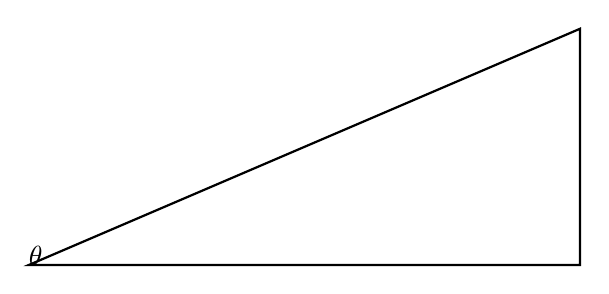
\begin{tikzpicture}[thick]
\coordinate (O) at (0,0);
\coordinate (A) at (7,0);
\coordinate (B) at (7,3);
\draw (O)--(A)--(B)--cycle;

%\tkzLabelSegment[below=2pt](O,A){\textit{adjacent leg}}
%\tkzLabelSegment[left=2pt](O,B){\textit{hypotenuse}}
%\tkzLabelSegment[above right=2pt](A,B){\textit{opposite leg}}

\tkzLabelSegment[below=5pt](O,A){\textit{x}}
\tkzLabelSegment[above left=5pt](O,B){\textit{r}}
\tkzLabelSegment[right=5pt](A,B){\textit{y}}

\tkzMarkAngle[fill= orange,size=1.5cm, opacity=.4](A,O,B)
\tkzLabelAngle[pos = 2](A,O,B){\texttt{$\theta$}}

% \tkzMarkAngle[fill= orange,size=0.65cm, opacity=.4](A,O,B)
% \tkzLabelAngle[pos = 0.35](A,O,B){$\gamma$}
%
% \tkzMarkAngle[fill= orange,size=0.8cm, opacity=.4](B,A,O)
% \tkzLabelAngle[pos = 0.6](B,A,O){$\alpha$}
%
% \tkzMarkAngle[fill= orange,size=0.7cm, opacity=.4](O,B,A)
% \tkzLabelAngle[pos = 0.5](O,B,A){$\beta$}

\end{tikzpicture}

\item Du har nytta av metoderna \code{math.cos(theta)} och \code{math.sin(theta)} vid omvandling från polära koordinater.

\item Attributet \code{negY} kommer att underlätta för dig när du på laborationen ska omvandla en punkt till fönsterkoordinater där y-axeln är omvänd jämfört med kartesiska koordinater.

\item Notera att klassens attribut är av typen \code{Double} och inte \code{Int}, trots att vi senare ska använda punkten för att beskriva en diskret pixelposition. Anledningen till detta är att det kan uppstå avrundningsfel vid numeriska beräkningar. Detta blir särskilt märkbart vid upprepad räkning med små värden, t.ex. när man ritar en approximerad cirkel med många linjesegment.
\end{itemize}

\SOLUTION

\TaskSolved \what~
\begin{Code}
package graphics

case class Point(x: Double, y: Double) {
  val r: Double          = math.hypot(x, y)
  val theta: Double      = math.atan2(y, x)
  def negY: Point        = Point(x, -y)
  def +(p: Point): Point = Point(x + p.x, y + p.y)
}
object Point {
  def polar(r: Double, theta: Double): Point =
    Point(r * math.cos(theta), r * math.sin(theta))
}
\end{Code}

\QUESTEND



\clearpage

\ExtraTasks %%%%%%%%%%%%%%%%%%%%%%%%%%%%%%%%%%%%%%%%%%%%%%%%%%%%%%%%%%%%%%%%%%%%



\WHAT{Instansiering med \code{new} och värdet \code{null}.}

\QUESTBEGIN

\Task  \what~  Man skapar instanser av klasser med \code{new}. Då anropas konstruktorn och plats reserveras i datorns minne för objektet. Variabler av referenstyp som inte refererar till något objekt har värdet \code{null}.

\Subtask Vad händer nedan? Vilka rader ger felmeddelande och i så fall hur lyder felmeddelandet?

\begin{REPL}
scala> class Gurka(val vikt: Int)
scala> var g: Gurka = null
scala> g.vikt
scala> g = new Gurka(42)
scala> g.vikt
scala> g = null
scala> g.vikt
\end{REPL}

\Subtask Rita minnessituationen efter raderna 2, 4, 6.

\SOLUTION


\TaskSolved \what


\SubtaskSolved  Rad 3 och 7 ger båda felmeddelandet \code{java.lang.NullPointerException},  på grund av försök att referera medlemmar med hjälp av en \code{null}-referens, som alltså inte pekar på något objekt.

\SubtaskSolved  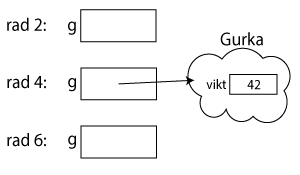
\includegraphics[scale=0.6]{../img/w06-solutions/1b}


\QUESTEND


\WHAT{Klasser,  instanser och skräp.}

\QUESTBEGIN

\Task  \what~För länge sedan i en galax långt långt borta...

\begin{Code}
case class Arm(ärTillVänster: Boolean)

case class Ben(ärTillVänster: Boolean)

case class Huvud(harHår: Boolean = true)

case class Rymdvarelse (
      arm1:   Arm   = Arm(true),
      arm2:   Arm   = Arm(false),
      ben1:   Ben   = Ben(true),
      ben2:   Ben   = Ben(false),
      huvud1: Huvud = Huvud(harHår = false),
  var huvud2: Huvud = Huvud()
) {
  def ärSkallig = !huvud1.harHår && !huvud2.harHår
}
\end{Code}

\Subtask Klistra in ovan rymdkod i REPL och evaluera nedan rader. Rita minnessituationen efter rad 5 och beskriv vad som händer.
\begin{REPL}
scala> val alien = Rymdvarelse()
scala> alien.ärSkallig
scala> val predator = Rymdvarelse()
scala> predator.ärSkallig
scala> predator.huvud2 = alien.huvud1
scala> predator.huvud2 eq alien.huvud1  // test av referenslikhet
scala> println(predator)
scala> predator.ärSkallig
\end{REPL}

\Subtask Vad händer så småningom med det ursprungliga \code{huvud2}-objektet i predator efter tilldelningen på rad 5? Går det att referera till detta objekt på något sätt?

\SOLUTION

\TaskSolved \what

\SubtaskSolved  Vi skapar två rymdvarelser, \code{alien} och \code{predator}, med vardera två ben och två armar, samt vardera två huvuden (där det ena är skalligt och det andra har hår). Efter det är varken \code{alien} eller \code{predator} skallig eftersom båda har ett huvud med hår. Sen låter man referensen till \code{predator}s huvud med hår referera till aliens huvud utan hår. Nu är predator helt skallig och delar huvud med alien.

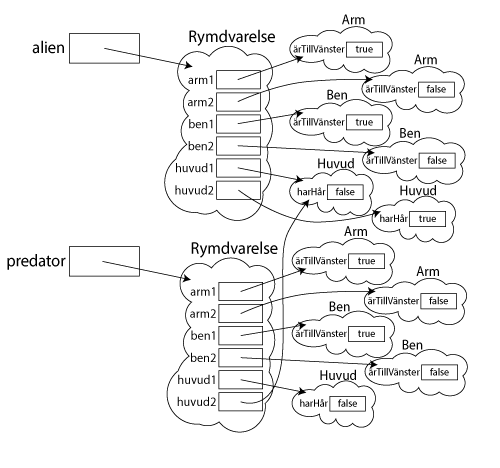
\includegraphics[scale=0.65]{../img/w06-solutions/2b}

\SubtaskSolved  Eftersom det inte längre finns någon referens som pekar på det objektet kommer skräpsamlaren att ta hand om det och det kommer förr eller senare skrivas över av något annat när platsen i minnet behövs. Objekt som inte har någon referens tills sig går inte att komma åt.

\QUESTEND




\WHAT{Case-klass. Oföränderlig kvadrat.}

\QUESTBEGIN

\Task \label{task:Square} \what~

\Subtask Implementera nedan kvadrat med en editor och klistra in den i REPL.

\begin{Code}
case class Square(val x: Int = 0, val y: Int = 0, val side: Int = 1) {
  val area: Int = ???

  /** Creates a new Square moved to position (x + dx, y + dy) */
  def moved(dx: Int, dy: Int): Square = ???

  def isEqualSizeAs(that: Square): Boolean = ???

  /** Multiplies the side with factor and rounded to nearest integer */
  def scale(factor: Double): Square = ???
}
object Square {
  /** A Square at (0, 0) with side 1 */
  val unit: Square = ???
}
\end{Code}

\Subtask Testa din kvadrat enligt nedan. Förklara vad som händer.

\begin{REPL}
scala> val (s1, s2) = (Square(), Square(1, 10, 1))
scala> val s3 = s1 moved (1,-5)
scala> s1 isEqualSizeAs s3
scala> s2 isEqualSizeAs s1
scala> s1 isEqualSizeAs Square.unit
scala> s2.scale(math.Pi) isEqualSizeAs s2
scala> s2.scale(math.Pi) isEqualSizeAs s2.scale(math.Pi)
scala> s2.scale(math.Pi) eq s2.scale(math.Pi)
scala> Square.unit eq Square.unit
\end{REPL}

\SOLUTION

\TaskSolved \what

\SubtaskSolved

\begin{Code}
case class Square(val x: Int = 0, val y: Int = 0, val side: Int = 1) {
	val area: Int = side * side

	def moved(dx: Int, dy: Int): Square = new Square(x + dx, y + dy, side)

	def isEqualSizeAs(that: Square): Boolean = this.side == that.side

	def scale(factor: Double): Square =
    Square(x, y, (side * factor).round.toInt)
}

object Square {
	val unit: Square = Square()
}
\end{Code}

\SubtaskSolved
\begin{REPL}
scala> val (s1, s2) = (Square(), Square(1, 10, 1))
s1: Square = Square(0,0,1)
s2: Square = Square(1,10,1)

scala> val s3 = s1 moved (1,-5)
s3: Square = Square(1,-5,1)

scala> s1 isEqualSizeAs s3       // lika storlek
res55: Boolean = true

scala> s2 isEqualSizeAs s1       // lika storlek
res56: Boolean = true

scala> s1 isEqualSizeAs Square.unit   // s1 har sidan 1
res57: Boolean = true

scala> s2.scale(math.Pi) isEqualSizeAs s2  // olika storlek
res58: Boolean = false

scala> s2.scale(math.Pi) == s2.scale(math.Pi) // lika innehåll
res59: Boolean = true

scala> s2.scale(math.Pi) eq s2.scale(math.Pi)  // olika objekt
res60: Boolean = false

scala> Square.unit eq Square.unit   // samma objekt
res61: Boolean = true
\end{REPL}

\QUESTEND



\WHAT{Förändrinsbar Java-klass.}

\QUESTBEGIN

\Task \what~Översätt nedan Scala-klass till Java-klassen \code{JMutablePoint3D}. Alla attribut ska vara privata (varför?). Översätt defaultargumentet till en alternativ konstruktor. Kalla setters för t.ex. \jcode{setX}. Kör \code{javac} och testa i REPL.

\begin{Code}
class MutablePoint3D(var x: Int, var y: Int, var z: Int = 0)
\end{Code}

\SOLUTION

\TaskSolved \what~

\javainputlisting[numbers=left]{examples/JMutablePoint3D.java}

\begin{REPL}
> atom JMutablePoint3D.java
> javac JMutablePoint3D.java
> ls
JMutablePoint3D.class  JMutablePoint3D.java
> scala
Welcome to Scala 2.12.3 (Java HotSpot(TM) 64-Bit Server VM, Java 1.8.0_121).
Type in expressions for evaluation. Or try :help.

scala> val p = new JMutablePoint3D(1,2)
p: JMutablePoint3D = JMutablePoint3D@2cae9b8

scala> p.x
<console>:13: error: value x is not a member of JPoint3D

scala> p.getZ
res0: Int = 0

scala> p.setZ(3)

scala> p.getZ
res1: Int = 3

\end{REPL}

\QUESTEND






\clearpage

\AdvancedTasks %%%%%%%%%%%%%%%%%%%%%%%%%%%%%%%%%%%%%%%%%%%%%%%%%%%%%%%%%%%%%%%%%


\WHAT{Attributrepresentation. Privat konstruktor. Fabriksmetod.}

\QUESTBEGIN

\Task \what~Kim Kodkunnig skapade för länge sedan denna klass som används på många ställen i befintlig kod:

\begin{Code}
class Point private (val x: Int, val y: Int)
object Point {
  def apply(x: Int = 0, y: Int = 0): Point = new Point(x, y)
  val origo = apply()
}
\end{Code}

\Subtask Vad händer om du försöker instansiera Kim Kodkunnigs klass direkt med nyckelordet \code{new}?

\Subtask Varför använder Kim Kodkunnig ett kompanjonsobjekt med en fabriksmetod? Vilka accessregler gäller mellan ett kompanjonsobjekt och klassen med samma namn?

\Subtask Hjälp Kim Kodkunnig att ändra attributrepresentationen så att det oföränderliga tillståndet utgörs av en 2-tupel \code{val p: (Int, Int)} i stället. Befintlig kod ska inte behöva ändras och klassen \code{Point} ska bete sig från ''utsidan'' precis som innan.

\SOLUTION

\TaskSolved \what~

\SubtaskSolved Det blir kompileringsfel eftersom konstruktorn är privat.
\begin{REPL}
scala> :paste

class Point private (val x: Int, val y: Int)
object Point {
  def apply(x: Int = 0, y: Int = 0): Point = new Point(x, y)
  val origo = apply()
}

scala> new Point(0,0)
<console>:14: error: constructor Point in class Point cannot be accessed
\end{REPL}

\SubtaskSolved
\begin{itemize}
  \item Genom att ha en privat konstruktor och bara göra indirekt instansiering via fabriksmetod är lätt ändra attributrepresentation i framtiden utan att befintlig kod behöver ändras.

  \item Med en \code{apply}-metod i kompansjonsobjektet kan man instansiera genom att skriva \code{Point(1, 2)} utan new.

  \item Accessreglerna för kompanjonsobjekt är sådana att kompanjoner ser varandras privata delar.
\end{itemize}

\SubtaskSolved

\begin{Code}
class Point private (private val p: (Int, Int)) {
  def x: Int = p._1
  def y: Int = p._2
}
object Point {
  def apply(x: Int = 0, y: Int = 0): Point = new Point(x, y)
  val origo = apply()
}
\end{Code}

\QUESTEND



\WHAT{Synlighet av klassparametrar och konstruktor, \code{private[this]}.}

\QUESTBEGIN

\Task  \what~

\Subtask En av gurk-klasserna nedan är trasig. Varför och vad blir det för fel?

\begin{Code}
class Gurka1(vikt: Int)

class Gurka2(val vikt: Int)

class Gurka3(private val vikt: Int)

class Gurka4(private val vikt: Int, kompis: Gurka4){
  def kompisVikt = kompis.vikt
}

class Gurka5(private[this] val vikt: Int, kompis: Gurka5){
  def kompisVikt = kompis.vikt
}

class Gurka6 private (vikt: Int)

class Gurka7 private (var vikt: Int)
object Gurka7 {
  def apply(vikt: Int) = {
    require(vikt >= 0, "negativ vikt: " + vikt)
    new Gurka7(vikt)
  }
}
\end{Code}

\Subtask Undersök nedan vad nyckelorden \code{val} och \code{private} får för konsekvenser. Förklara vad som händer. Vilka rader ger vilka felmeddelanden?

\begin{REPL}
scala> new Gurka1(42).vikt
scala> new Gurka2(42).vikt
scala> new Gurka3(42).vikt
scala> val ingenGurka: Gurka4 = null
scala> new Gurka4(42, ingenGurka).kompisVikt
scala> new Gurka4(42, new Gurka4(84, null)).kompisVikt
scala> new Gurka6(42)
scala> new Gurka7(-42)
scala> Gurka7(-42)
scala> val g = Gurka7(42)
scala> g.vikt
scala> g.vikt = -1
scala> g.vikt
\end{REPL}


\SOLUTION


\TaskSolved \what

\SubtaskSolved \code{Gurka5} är trasig. Eftersom vikten i \code{Gurka5} är privat för instansen och inte klassen kan en instans inte accessa en annan instans vikt.
\begin{REPL}
  error: value vikt is not a member of Gurka5
  def kompisVikt = kompis.vikt
\end{REPL}


\SubtaskSolved
\begin{REPL}
scala> new Gurka1(42).vikt
<console>:13: error: value vikt is not a member of Gurka1
       new Gurka1(42).vikt
                      ^

scala> new Gurka2(42).vikt
res64: Int = 42

scala> new Gurka3(42).vikt
<console>:13: error: value vikt in class Gurka3 cannot be accessed in Gurka3
       new Gurka3(42).vikt
                      ^

scala> val ingenGurka: Gurka4 = null
ingenGurka: Gurka4 = null

scala> new Gurka4(42, ingenGurka).kompisVikt
java.lang.NullPointerException
  at Gurka4.kompisVikt(<console>:13)
  ... 36 elided

scala> new Gurka4(42, new Gurka4(84, null)).kompisVikt
res67: Int = 84

scala> new Gurka6(42)
<console>:13: error: constructor Gurka6 in class Gurka6 cannot be accessed
       new Gurka6(42)
       ^

scala> new Gurka7(-42)
<console>:14: error: constructor Gurka7 in class Gurka7 cannot be accessed
       new Gurka7(-42)
       ^

scala> Gurka7(-42)
java.lang.IllegalArgumentException: requirement failed: negativ vikt: -42


scala> val g = Gurka7(42)
g: Gurka7 = Gurka7@70717ed5

scala> g.vikt
res71: Int = 42

scala> g.vikt = -1
g.vikt: Int = -1

scala> g.vikt
res72: Int = -1
\end{REPL}

\QUESTEND





\WHAT{Egendefinierad setter kombinerat med privat konstruktor.}

\QUESTBEGIN

\Task  \what~Klistra in denna kod i REPL:

\begin{Code}
class Gurka8 private (private var _vikt: Int) {
  def vikt = _vikt
  def vikt_=(v: Int): Unit = {
    require(v >= 0, "negativ vikt: " +v)
    _vikt = v
  }
}

object Gurka8 {
  def apply(vikt: Int) = {
    require(vikt >= 0, "negativ vikt: " + vikt)
    new Gurka8(vikt)
  }
}
\end{Code}


\Subtask Förklara vad som händer nedan. Vilka rader ger vilka felmeddelanden?
\begin{REPL}
scala> val g = Gurka8(-42)
scala> val g = Gurka8(42)
scala> g.vikt
scala> g.vikt = 0
scala> g.vikt = -1
scala> g.vikt += 42
scala> g.vikt -= 1000
\end{REPL}

\Subtask Vad är fördelen med möjligheten att skapa egendefinierade setters?

\SOLUTION


\TaskSolved \what


\SubtaskSolved

Rad 1:
\begin{REPL}
	java.lang.IllegalArgumentException: requirement failed: negativ vikt: -42
\end{REPL}
\code{Gurka8.apply} kräver att \code{vikt >= 0} annars kastar \code{require} ett undantag.

Rad 5:
\begin{REPL}
	java.lang.IllegalArgumentException: requirement failed: negativ vikt: -1
\end{REPL}
Settern \code{vikt_=} kräver att \code{vikt >= 0} annars kastar \code{require} ett undantag.

Rad 7:
\begin{REPL}
	java.lang.IllegalArgumentException: requirement failed: negativ vikt: -958
\end{REPL}
Eftersom \code{42 - 1000} är mindre än noll kastar \code{require} ett undantag.

\SubtaskSolved  Man kan sätta egna mer specifika krav på vad som får göras med värdena så man har större koll på att inget oväntat händer.

\QUESTEND




\WHAT{Objekt med föränderligt tillstånd \Eng{mutable state}.}

\QUESTBEGIN

\Task  \what~  Du ska implementera en modell av en hoppande groda som uppfyller följande krav:
\begin{enumerate}%[nolistsep, noitemsep]
\item Varje grodobjekt ska hålla reda på var den är.
\item Varje grodobjekt ska hålla reda på hur långt grodan hoppat totalt.
\item Varje grodobjekt ska kunna beräkna hur långt det är mellan grodans nuvarande position och utgångsläget.
\item Alla grodor börjar sitt hoppande i origo.
\item En groda kan hoppa enligt två metoder:
  \begin{itemize} [nolistsep, noitemsep]
  \item relativ förflyttning enligt parametrarna \code{dx} och \code{dy},
  \item slumpmässig relativ förflyttning $[1, 10]$ i x-ledsförändring och $[1, 10]$ i y-ledsförändring.
  \end{itemize}
\end{enumerate}

\Subtask Implementera klassen \code{Frog} enligt nedan kodskelett och ovan krav.

\begin{Code}
class Frog private (initX: Int = 0, initY: Int = 0) {
  def x: Int = ???
  def y: Int = ???

  def jump(dx: Int, dy: Int): Unit = ???
  def randomJump: Unit = ???

  def distanceToStart: Double = ???
  def distanceJumped: Double = ???
  def distanceTo(that: Frog): Double = ???
}
object Frog {
  def spawn(): Frog = ???
}
\end{Code}
\emph{Tips:}
\begin{itemize} [nolistsep, noitemsep]
\item Om namnet man vill ge ett privat föränderligt attribut ''krockar'' med ett metodnamn, är det vanligt att man börjar attributets namn med understreck, t.ex. \code{private var _x } för att på så sätt undkomma namnkonflikten.
\item Inför en metod i taget och klistra in den nya grodan i REPL efter varje utvidgning och testa.
\end{itemize}



\Subtask Skapa en metod \code{def test(): Unit} i ett singelobjekt \code{FrogTest} som innehåller kod som gör minst en kontroll av varje krav. Om ingen kontroll går fel ska \code{"Test Ok!"} skrivas ut annars ska exekveringen avbrytas. \emph{Tips:} Använd \code{assert(b, msg)} som avbryter exekveringen och skriver ut \code{msg} om \code{b} är falsk.

\Subtask Vad kallas en metod som enbart returnerar värdet av ett privat attribut?

\Subtask Inför setters för attributen som håller reda på x- och y-postitionen. Förändringar av positionen i x- eller y-led ska räknas som ett hopp och alltså registreras i det attribut som håller reda på det ackumulerade hoppavståndet.

\Subtask Simulera ett massivt grodhoppande med krockdetektering genom att skapa 100 grodor som till att börja med är placerade på x-axeln med avståndet $8$ längdenheter mellan sig. För varje runda i en \code{while}-sats, låt en slumpässigt vald groda göra ett \code{randomJump} tills någon groda befinner sig närmare än $0.5$ längdenheter, vilket är definitionen på att de har krockat. Räkna hur många looprundor som behövs innan något grodpar krockar och skriv ut antalet. Skriv även ut det totala antalet \\ \emph{Tips:} Börja med pseudokod på papper. Använd en grodvektor.


\SOLUTION


\TaskSolved \what


\SubtaskSolved
\begin{Code}
class Frog private (initX: Int = 0, initY: Int = 0) {
	private var _x: Int = initX
	private var _y: Int = initY
	private var _distanceJumped: Double = 0

  def x: Int = _x
  def y: Int = _y

	def jump(dx: Int, dy: Int): Unit = {
		_x += dx
		_y += dy
		_distanceJumped += math.hypot(dx, dy)
	}


	def randomJump: Unit = {
		def rnd = util.Random.nextInt(10) + 1
		jump(rnd, rnd)
	}

	def distanceToStart: Double = math.hypot(x,y)
	def distanceJumped: Double = _distanceJumped
	def distanceTo(f: Frog): Double = math.hypot(x - f.x, y - f.y)
}

object Frog {
	def spawn(): Frog = new Frog()
}
\end{Code}

\SubtaskSolved Exempel på testprogram:
\begin{Code}
object FrogTest {
  def test(): Unit = {
    val f1 = Frog.spawn()
    assert(f1.x == 0 && f1.y == 0, "Test of spawn, reqt 1 & 4 failed.")

    f1.jump(4,3)
    assert(f1.x == 4 && f1.y == 3, "Test of jump, reqt 1 & 4 failed.")

    f1.jump(4,3)
    assert(f1.distanceJumped == 10, "Test of jump, reqt 2 failed.")

    f1.jump(-4,-3)
    assert(f1.distanceToStart == 5, "Test of jump, reqt 3 failed.")

    for (x <- 1 to 10000) {
      val f2 = Frog.spawn()
    	f2.randomJump
    	assert(f2.x > 0 && f2.x <= 10 && f2.y > 0 && f2.y <= 10,
            "Test of randomJump, reqt 5 failed.")
    }
    println("Test Ok!")
  }
}
\end{Code}

\SubtaskSolved  En metod som är en indirekt avläsning av attrubtvärden kallas getter.

\SubtaskSolved
\begin{Code}

class Frog private (initX: Int = 0, initY: Int = 0) {
	private var _x: Int = initX
	private var _y: Int = initY
	private var _distanceJumped: Double = 0

	def jump(dx: Int, dy: Int): Unit = {
		_x += dx
		_y += dy
		_distanceJumped += math.hypot(dx, dy)
	}

	def x: Int = _x
  def x_= (newX: Int): Unit = { // Setter för x
		_distanceJumped += math.abs(x - newX)
		_x = newX
	}

  def y: Int = _y
	def y_= (newY: Int): Unit = { // Setter för y
		_distanceJumped += math.abs(y - newY)
		_y = newY
	}


	def randomJump: Unit = {
		def rnd = util.Random.nextInt(10) + 1
		jump(rnd, rnd)
	}

	def distanceToStart: Double = math.hypot(x,y)
	def distanceJumped: Double = _distanceJumped
	def distanceTo(f: Frog): Double = math.hypot(x - f.x, y - f.y)
}

object Frog {
	def spawn(): Frog = new Frog()
}

\end{Code}

\SubtaskSolved
\begin{Code}
object frogSimulation {
  def isAnyCollision(frogs: Vector[Frog]): Boolean = {
    var found = false
    frogs.indices.foreach { i =>  // generate all pairs (i,j)
      for (j <- i + 1 until frogs.size)
        if (!found) found = frogs(i).distanceTo(frogs(j)) <= 0.5
    }
    found
  }

  def jumpUntilCrash(n: Int = 100, initDist: Int = 8): (Int, Double) = {
    val frogs = Vector.fill(n)(Frog.spawn)
    (0 until n).foreach(i => frogs(i).x = i * initDistance)
    var count = 0
    while (!isAnyCollision(frogs)) {
      frogs(util.Random.nextInt(n)).randomJump
    	count += 1
    }
    (count, frogs.map(_.distanceJumped).sum)
  }

  def run(nbrOfCrashTests: Int = 10) = for (i <- 1 to nbrOfCrashTests) {
    val (n, dist) = jumpUntilCrash()
    println(s"\nAntalet looprundor innan grodkrock: $n")
    println(s"Totalt avstånd hoppat av alla grodor: $dist")
  }
}
\end{Code}

\QUESTEND




\QUESTBEGIN

\Task  \what~  Webbshoppen \textbf{UberSquare} säljer flyttbara kvadrater. I affärsmodellen ingår att ta betalt per förflyttning. Du ska hjälpa UberSquare att utveckla en enkel prototyp för att imponera på riskkapitalister.

\Subtask Implementera \code{Square} enligt dokumentationskommentarerna i efterföljande kodskiss och enligt dessa krav:

\begin{enumerate}%[nolistsep, noitemsep]
   \item Varje instans av \code{Square} ska räkna antalet förflyttningar som gjorts sedan instansen konstruerats.

   \item För att kunna övervaka sina kunder vill UberSquare även räkna det totala antalet förflyttningar som gjorts av alla kvadrater som någonsin skapats (s.k. \emph{big data}).

  \item Varje gång förflyttning sker ska ett visst belopp adderas till den ackumulerade kostnaden för respektive kvadrat, enligt kostnadsberäkningen i krav 4.

  \item UberSquare är oroliga för att kvadraterna flyttas för långt bort och bestämmer därför att för varje förflyttning ska den ackumulerade kvadratkostnaden ökas med den nya positionens avstånd till ursprungsläget vid kvadratens konstruktion multiplicerat med aktuell storlek på kvadraten.

  \item För att framstå som goda berättar UberSquare i sin marknadsföring att skala är gratis att använda. \footnote{D.v.s ett anrop av metoden \code{scale} orsakar ingen omedelbar kostnad.}
\end{enumerate}

\begin{CodeSmall}
/** A mutable and expensive Square. */
class Square private (val initX: Int, val initY: Int, val initSide: Int) {
  private var nMoves = 0;
  private var sumCost = 0.0;

  private var _x = initX;
  private var _y = initY;

  private var _side = initSide;

  private def addCost(): Unit = {
   sumCost += ???
  }

  def x: Int = ???
  def y: Int = ???

  def side = ???

  /** Scales the side of this square and rounds it to nearest integer */
  def scale(factor: Double): Unit = ???

  /** Moves this square to position (x + xd, y + dy) */
  def move(dx: Int, dy: Int): Unit = ???

  /** Moves this square to position (x, y) */
  def moveTo(x: Int, y: Int): Unit = ???

  /** The accumulated cost of this Square */
  def cost: Double = ???

  /** Returns the accumulated cost. Sets the accumulated cost to zero. */
  def pay: Double = ???

  override def toString: String =
    s"Square[($x, $y), side: $side, #moves: $nMoves times, cost: $sumCost]"
}


object Square {
  private var created = Vector[Square]()

  /** Constructs a new Square object at (x, y) with size side */
  def apply(x: Int, y: Int, side: Int): Square = {
    require(side >= 0, s"side must be positive: $side")
    ???
  }

  /** Constructs a new Square object at (0, 0) with side 1 */
  def apply(): Square = ???

  /** The total number of moves that have been made for all squares. */
  def totalNumberOfMoves: Int = ???

  /** The total cost of all squares. */
  def totalCost: Double = ???
}
\end{CodeSmall}

\Subtask Testa din kvadratprototyp i REPL. Använd t.ex. koden nedan:
\begin{REPL}
scala> val xs = Vector.fill(10)(Square())
scala> xs.foreach(_.move(2, 3))
scala> xs.foreach(_.scale(2.9))
scala> val (m, c) = (Square.totalNumberOfMoves, Square.totalCost)
m: Int = 10
c: Double = 36.055512754639885
\end{REPL}

\SOLUTION

\TaskSolved \what~

\begin{CodeSmall}
class Square private (val initX: Int, val initY: Int, val initSide: Int) {
  private var nMoves = 0;
  private var sumCost = 0.0;

  private var _x = initX;
  private var _y = initY;

  private var _side = initSide;

  private def addCost(): Unit = {
   sumCost += math.hypot(x - initX, y - initY) * side
  }

  def x: Int = _x
  def y: Int = _y

  def side = _side

  def scale(factor: Double): Unit = { _side = (_side * factor).round.toInt }

  def move(dx: Int, dy: Int): Unit = {
    _x += dx; _y += dy;
    nMoves += 1
    addCost()
  }

  def moveTo(x: Int, y: Int): Unit = {
    _x = x; _y = y;
    nMoves += 1
    addCost()
  }

  def cost: Double = sumCost

  def pay: Double = {val temp = sumCost; sumCost = 0; temp}

  override def toString: String =
    s"Square[($x, $y), side: $side, #moves: $nMoves times, cost: $sumCost]"
}
object Square {
  private var created = Vector[Square]()

  def apply(x: Int, y: Int, side: Int): Square = {
    require(side >= 0, s"side must be positive: $side")
    val sq = (new Square(x, y, side))
    created :+= sq
    sq
  }

  def apply(): Square = apply(0, 0, 1)

  def totalNumberOfMoves: Int = created.map(_.nMoves).sum

  def totalCost: Double = created.map(_.cost).sum
}
\end{CodeSmall}

\QUESTEND



\WHAT{Hjälpkonstruktor.}

\QUESTBEGIN

\Task\Uberkurs \label{task:aux-constructor} \what~I tidigare uppgifter har vi möjliggjort alternativa sätt att skapa instanser genom default-argument och fabriksmetoder i kompanjonsobjekt.

Ett annat sätt att göras detta på, som i Scala är ovanligt\footnote{Men i Java är detta mycket vanligt då defaultargument m.m. inte ingår i språket.}, är att definiera flera konstruktorer inne i klasskroppen. I Scala kallas en sådan extra konstruktor för \textbf{hjälpkonstruktor} \Eng{auxiliary constructor}.

En hjälpkonstruktor skapar man i Scala genom att definiera en metod som har det speciella namnet \code{this}, alltså en deklaration \code{def this(...) = ...} Hjälpkonstruktorer måste börja med att anropa en annan konstruktor, antingen den primära konstruktorn (d.v.s. den som klasshuvudet definierar) eller en tidigare definierad  hjälpkonstruktor.

\Subtask Läs mer om hjälpkonstruktorer här: \\ \href{http://www.artima.com/pins1ed/functional-objects.html#6.7}{www.artima.com/pins1ed/functional-objects.html\#6.7}

\Subtask Hitta på en egen uppgift med hjälpkonstruktorer, baserat på någon av klasserna i tidigare övningar.


%\Task \TODO \\ \code{class Rational private (numerator: BigInt, denominator: BigInt)} \\
%Inspirerat av Rational i pins1ed med GCD\SOLUTION

\QUESTEND


%!TEX encoding = UTF-8 Unicode
%!TEX root = ../exercises.tex

\ifPreSolution


\Exercise{\ExeWeekSIX}\label{exe:W06}

\begin{Goals}
%!TEX encoding = UTF-8 Unicode
%!TEX root = ../compendium2.tex

\item Kunna läsa och skriva pseudokod för sekvensalgoritmer och implementera sekvensalgoritmer enligt pseudokod.

\item Kunna implementera sekvensalgoritmer, både genom kopiering till ny sekvens och genom förändring på plats i befintlig sekvens.

\item Kunna använda inbyggda metoder för uppdatering av, linjärsökning i, och sortering av sekvenssamlingar.

\item Kunna beskriva skillnaden i användningen av föränderliga och oföränderliga sekvenser, speciellt vid uppdatering.

\item Kunna implementera linjärsökning enligt olika sökkriterier.

\item Kunna beskriva egenskaperna hos sekvenssamlingarna \code{Vector}, \code{List}, \code{Array}, \code{ArrayBuffer} och \code{ListBuffer}.

\item Förstå bieffekter av uppdatering av delade referenser till föränderliga element.

\item Kunna använda funktioner med repeterade parametrar.

\item Känna till hur man implementerar funktioner med repeterade parametrar.

\item Kunna implementera heltalsregistrering i en heltalsarray.

\item Kunna beskriva skillnader i syntax mellan arrayer i Scala och Java.

\item Kunna beskriva skillnader i syntax och semantik mellan enkla for-satser i Scala och Java.


\item Känna till hur klassen \code{java.util.Scanner} kan användas för att skapa heltalssekvenser ur strängsekvenser.

\end{Goals}

\begin{Preparations}
\item \StudyTheory{06}
\end{Preparations}

\else

\ExerciseSolution{\ExeWeekSIX}

\fi


\BasicTasks %%%%%%%%%%%



\WHAT{Para ihop begrepp med beskrivning.}

\QUESTBEGIN

\Task \what

\vspace{1em}\noindent Koppla varje begrepp med den (förenklade) beskrivning som passar bäst:

\begin{ConceptConnections}
  samlingsbibliotek & 1 & & A & algoritm som leta upp element enligt sökkriterium \\ 
  sekvenssamling & 2 & & B & många färdiga datastrukturer med olika egenskaper \\ 
  sekvensalgoritm & 3 & & C & algoritm som ordnar element i en viss ordning \\ 
  ordning & 4 & & D & algoritm som räknar element med vissa egenskaper \\ 
  sortering & 5 & & E & beskriver hur element av en viss typ ska ordnas \\ 
  söking & 6 & & F & lösning på problem som drar nytta av sekvenser \\ 
  registrering & 7 & & G & variabelt antal argument, asterisk efter parametertyp \\ 
  varargs & 8 & & H & noll el. flera element av samma typ i viss ordning \\ 
\end{ConceptConnections}

\SOLUTION

\TaskSolved \what

\begin{ConceptConnections}
  samlingsbibliotek & 1 & ~~\Large$\leadsto$~~ &  H & många färdiga datastrukturer med olika egenskaper \\ 
  sekvenssamling & 2 & ~~\Large$\leadsto$~~ &  F & noll el. flera element av samma typ i viss ordning \\ 
  sekvensalgoritm & 3 & ~~\Large$\leadsto$~~ &  D & lösning på problem som drar nytta av sekvenser \\ 
  ordning & 4 & ~~\Large$\leadsto$~~ &  C & beskriver hur element av en viss typ ska ordnas \\ 
  sortering & 5 & ~~\Large$\leadsto$~~ &  E & algoritm som ordnar element i en viss ordning \\ 
  söking & 6 & ~~\Large$\leadsto$~~ &  B & algoritm som leta upp element enligt sökkriterium \\ 
  registrering & 7 & ~~\Large$\leadsto$~~ &  G & algoritm som räknar element med vissa egenskaper \\ 
  varargs & 8 & ~~\Large$\leadsto$~~ &  A & variabelt antal argument, asterisk efter parametertyp \\ 
\end{ConceptConnections}

\QUESTEND



\WHAT{Olika sekvenssamlingar.}

\QUESTBEGIN

\Task \what~Koppla varje sekvenssamling med den (förenklade) beskrivning som passar bäst:

\begin{ConceptConnections}
  \code|Vector     | & 1 & & A & förändringsbar, snabb att ändra i början \\ 
  \code|List       | & 2 & & B & förändringsbar, snabb indexering, kan ändra storlek \\ 
  \code|Array      | & 3 & & C & oföränderlig, ger snabbt ny samling ändrad i början \\ 
  \code|ArrayBuffer| & 4 & & D & primitiv, förändringsbar, snabb indexering, fix storlek \\ 
  \code|ListBuffer | & 5 & & E & oföränderlig, ger snabbt godtyckligt ändrad samling \\ 
\end{ConceptConnections}

\SOLUTION

\TaskSolved \what

\begin{ConceptConnections}
  \code|Vector     | & 1 & ~~\Large$\leadsto$~~ &  C & oföränderlig, ger snabbt godtyckligt ändrad samling \\ 
  \code|List       | & 2 & ~~\Large$\leadsto$~~ &  D & oföränderlig, ger snabbt ny samling ändrad i början \\ 
  \code|Array      | & 3 & ~~\Large$\leadsto$~~ &  E & primitiv, förändringsbar, snabb indexering, fix storlek \\ 
  \code|ArrayBuffer| & 4 & ~~\Large$\leadsto$~~ &  B & förändringsbar, snabb indexering, kan ändra storlek \\ 
  \code|ListBuffer | & 5 & ~~\Large$\leadsto$~~ &  A & förändringsbar, snabb att ändra i början \\ 
\end{ConceptConnections}

\QUESTEND




\WHAT{Typer i hierarkin av sekvenssamlingar.}

\QUESTBEGIN

\Task \what~Koppla varje typ i hierarkin av sekvenssamling med den (förenklade) beskrivning som passar bäst:

\begin{ConceptConnections}
  Traversable & 1 & & A & bastyp för alla sekvenssamlingar, indexposition från 0 \\ 
  Iterable & 2 & & B & bastyp för alla samlingar, har metoden \code|foreach| \\ 
  Seq & 3 & & C & är traverserbar med hjälp av metoden \code|iterator| \\ 
\end{ConceptConnections}

\SOLUTION

\TaskSolved \what

\begin{ConceptConnections}
  Traversable & 1 & ~~\Large$\leadsto$~~ &  A & bastyp för alla samlingar, har metoden \code|foreach| \\ 
  Iterable & 2 & ~~\Large$\leadsto$~~ &  C & är traverserbar med hjälp av metoden \code|iterator| \\ 
  Seq & 3 & ~~\Large$\leadsto$~~ &  B & bastyp för alla sekvenssamlingar, indexposition från 0 \\ 
\end{ConceptConnections}

\QUESTEND


\WHAT{Använda sekvenssamlingar.}

\QUESTBEGIN

\Task \what~Antag att nedan variabler finns synliga i aktuell namnrymd:
\begin{Code}
val xs: Vector[Int] = Vector(1, 2, 3)
val x: Int = 0
\end{Code}

\Subtask Koppla varje uttryck till vänster med motsvarande resultat till höger. Om du är osäker på resultatet, läs i snabbreferensen och testa i REPL. \\\emph{Tips: ''colon on the collection side''}.

\begin{ConceptConnections}
  \code|x +: xs         | & 1 & & A & \code|Vector(1, 2, 3)                         | \\ 
  \code|xs +: x         | & 2 & & B & \code|true                                    | \\ 
  \code|xs :+ x         | & 3 & & C & \code|(0 until 3)                             | \\ 
  \code|xs ++ xs        | & 4 & & D & \code|Vector(1, 2, 3, 1, 2, 3)                | \\ 
  \code|xs.indices      | & 5 & & E & \code|1                                       | \\ 
  \code|xs apply 0      | & 6 & & F & \code|3                                       | \\ 
  \code|xs(3)           | & 7 & & G & \code|Vector(1, 2, 3, 0)                      | \\ 
  \code|xs.length       | & 8 & & H & \code|Vector(0, 1, 2, 3)                      | \\ 
  \code|xs.take(4)      | & 9 & & I & \code|2                                       | \\ 
  \code|xs.drop(2)      | & 10 & & J & \code|error: value +: is not a member of Int  | \\ 
  \code|xs.updated(0, 2)| & 11 & & K & \code|Vector(2, 2, 3)                         | \\ 
  \code|xs.tail.head    | & 12 & & L & \code|error: value tail is not a member of Int| \\ 
  \code|xs.head.tail    | & 13 & & M & \code|java.lang.IndexOutOfBoundsException     | \\ 
  \code|xs.isEmpty      | & 14 & & N & \code|false                                   | \\ 
  \code|xs.nonEmpty     | & 15 & & O & \code|Vector(3)                               | \\ 
\end{ConceptConnections}

\Subtask Vid tre tillfällen blir det fel. Varför? Är det kompileringsfel eller exekveringsfel?



\begin{framed}
\noindent\emph{Tips inför fortsättningen:}
Scalas standardbibliotek har många användbara samlingar med enhetlig metoduppsättning. Om du lär dig de viktigaste samlingsmetoderna får du en mångsidig och kraftfull verktygslåda. Läs mer här:

    \begin{itemize}%[nolistsep]
      \item snabbreferensen (enda tentahjälpmedel): \\{\small\url{http://cs.lth.se/pgk/quickref}}
      \item översikt (av Prof. Martin Odersky, uppfinnare av Scala): \\
       {\small\url{http://docs.scala-lang.org/overviews/collections/introduction.html}}
      \item api-dokumentation:\\  {\small\url{https://www.scala-lang.org/api/current/scala/collection/}}
    \end{itemize}
\end{framed}



\SOLUTION

\TaskSolved \what

\SubtaskSolved

\begin{ConceptConnections}
  \code|x +: xs         | & 1 & ~~\Large$\leadsto$~~ &  H & \code|Vector(0, 1, 2, 3)                      | \\ 
  \code|xs +: x         | & 2 & ~~\Large$\leadsto$~~ &  J & \code|error: value +: is not a member of Int  | \\ 
  \code|xs :+ x         | & 3 & ~~\Large$\leadsto$~~ &  G & \code|Vector(1, 2, 3, 0)                      | \\ 
  \code|xs ++ xs        | & 4 & ~~\Large$\leadsto$~~ &  D & \code|Vector(1, 2, 3, 1, 2, 3)                | \\ 
  \code|xs.indices      | & 5 & ~~\Large$\leadsto$~~ &  C & \code|(0 until 3)                             | \\ 
  \code|xs apply 0      | & 6 & ~~\Large$\leadsto$~~ &  E & \code|1                                       | \\ 
  \code|xs(3)           | & 7 & ~~\Large$\leadsto$~~ &  M & \code|java.lang.IndexOutOfBoundsException     | \\ 
  \code|xs.length       | & 8 & ~~\Large$\leadsto$~~ &  F & \code|3                                       | \\ 
  \code|xs.take(4)      | & 9 & ~~\Large$\leadsto$~~ &  A & \code|Vector(1, 2, 3)                         | \\ 
  \code|xs.drop(2)      | & 10 & ~~\Large$\leadsto$~~ &  O & \code|Vector(3)                               | \\ 
  \code|xs.updated(0, 2)| & 11 & ~~\Large$\leadsto$~~ &  K & \code|Vector(2, 2, 3)                         | \\ 
  \code|xs.tail.head    | & 12 & ~~\Large$\leadsto$~~ &  I & \code|2                                       | \\ 
  \code|xs.head.tail    | & 13 & ~~\Large$\leadsto$~~ &  L & \code|error: value tail is not a member of Int| \\ 
  \code|xs.isEmpty      | & 14 & ~~\Large$\leadsto$~~ &  N & \code|false                                   | \\ 
  \code|xs.nonEmpty     | & 15 & ~~\Large$\leadsto$~~ &  B & \code|true                                    | \\ 
\end{ConceptConnections}

\SubtaskSolved

\noindent\renewcommand*{\arraystretch}{1.2}\begin{tabular}{p{5cm} l p{6cm}}

~\\ \emph{fel} & \emph{typ} & \emph{förklaring} \\\hline

\code|error: value +: is| \code|not a member of Int|
& kompileringsfel
& Operatorer som slutar med kolon är högerassociativa. Metodanropet \code|xs +: x| motsvarar med punktnotation \code|x.+:(xs)| och det finns ingen metod med namnet \code|+:| på heltal.\\\hline

\code|IndexOutOfBoundsException|
& körtidsfel & Det finns bara 3 element och index räknas från 0 i sekvenssamlingar.\\\hline

\code|error: value tail is | \code|not a member of Int|
& kompileringsfel
& Metoden \code|head| ger första elementet och heltal saknar sekvenssamlingsmetoden \code|tail|.\\\hline

\end{tabular}


\QUESTEND


\WHAT{Inbyggda metoder för kopiering av sekvenser.}

\QUESTBEGIN

\Task \what~ \code{map} \code{toArray} \code{copyToArray}

\Subtask Uppdatering av oföränderliga sekvenser. \TODO

\Subtask Uppdatering av förändringsbara sekvenser. \TODO

\SOLUTION

\TaskSolved \what~\TODO

\QUESTEND



\WHAT{Inbyggda metoder för uppdatering av sekvenser.}

\QUESTBEGIN

\Task \what~ \code{updated} \code{update} \code{+=} \code{patch}

\Subtask Uppdatering av oföränderliga sekvenser. \TODO

\Subtask Implementera insert på Vector med hjälp av patch. \TODO

\Subtask Uppdatering av förändringsbara sekvenser. \TODO

\SOLUTION

\TaskSolved \what~\TODO

\QUESTEND




\WHAT{Inbyggda metoder för linjärsökning.}

\QUESTBEGIN

\Task \what~\TODO

\SOLUTION

\TaskSolved \what~\TODO

\QUESTEND

\WHAT{Inbyggda metoder för sortering.}

\QUESTBEGIN

\Task \what~\TODO



\SOLUTION

\TaskSolved \what~\TODO

\QUESTEND


\ifPreSolution
\begin{framed}
\noindent\emph{Tips inför fortsättningen:} Även om man normalt kan lösa grundläggande delproblem med inbyggda samlingsmetoder ur standardbiblioteket, är det mycket bra för förståelsen att kunna implementera grundläggande sekvensalgoritmer. Du ska därför i kommande uppgifter träna på att implementera algoritmer att skapa funktioner som gör liknande saker som redan finns färdigt i standardbiblioteket.
\end{framed}
\fi



\WHAT{Implementera.}

\QUESTBEGIN

\Task \what~\TODO

\SOLUTION

\TaskSolved \what~\TODO

\QUESTEND



\WHAT{Implementera registrering med hjälp av Array. LABBFÖRBEREDELSE.}

\QUESTBEGIN

\Task \what~Räkna tärningskas\TODO

\SOLUTION

\TaskSolved \what~\TODO

\QUESTEND






\ExtraTasks %%%%%%%%%%%%%%%%%%%%%%%%%%%%%%%%%%%%%%%%%%%%%%%%%%%%%%%%%%%%%%%%%%%%



\AdvancedTasks %%%%%%%%%%%%%%%%%%%%%%%%%%%%%%%%%%%%%%%%%%%%%%%%%%%%%%%%%%%%%%%%%



\subsection{\TODO Värdera nedan gamla uppgifter}


\WHAT{Variabelt antal argument.}

\QUESTBEGIN

\Task  \what~  Det går fint att deklarera en funktion som tar en argumentsekvens av godtycklig längd. Syntaxen består av en asterisk \code{*} efter typen.

\Subtask Vad händer nedan?
\begin{REPL}
scala> def printAll(xs: Int*) = xs.foreach(println)
scala> printAll(42)
scala> printAll(1, 2, 7, 42)
scala> def printStrings(wa: String*) = println(wa)
scala> printStrings("hej","på","dej")
\end{REPL}

\Subtask Vad har parametern \code{wa} i \code{printStrings} ovan för typ?

\Subtask Ändra i \code{printAll} så att även längden på \code{xs} skrivs ut före utskriften av alla element. Testa att anropa \code{printAll} med olika antal parametrar.

\Subtask Vad händer om du anropar \code{printAll} med noll parametrar?

\SOLUTION


\TaskSolved \what


\SubtaskSolved  42;\\
 1\\
 2\\
 7\\
 42;\\
 WrappedArray(hej, på, dej)

\SubtaskSolved  WrappedArray

\SubtaskSolved  def printAll(xs: Int*) = {println(xs.size); xs.foreach(println)}

\SubtaskSolved  Storleken “0” skrivs ut och inget annat.




\QUESTEND




%%<AUTOEXTRACTED by mergesolu>%%      % Uppgift 1




\WHAT{Oföränderliga sekvenser med föränderliga objekt.}

\QUESTBEGIN

\Task  \what~

\Subtask Vad får xs för värde efter att attributet i objektet som \code{c2} refererar till ändras på rad 4 nedan? Förklara vad som händer.
\begin{REPL}
scala> class IntCell(var x: Int){override def toString = "[Int](" + x + ")"}
scala> val (c1, c2, c3) = (new IntCell(7), new IntCell(8), new IntCell(9))
scala> val xs = Vector(c1, c2, c3)
scala> c2.x = 42
scala> xs
\end{REPL}

\Subtask\Pen Rita en bild av minnessituationen efter rad 4 ovan.

\Subtask\Pen Vad krävs för att allt innehåll i en oföränderlig samling garanterat ska förbli oförändrat?

\SOLUTION


\TaskSolved \what


\SubtaskSolved  \begin{REPL}
scala.collection.immutable.Vector[IntCell] =
    Vector([Int](7), [Int](42), [Int](9))
\end{REPL}
Referensena till c2 och xs ändras aldrig.
xs kommer fortfarande ha tre vektorer som refererar till c1, c2, c3, däremot refererar dessa i sin tur till var sin int som är Mutable.
I detta fallet ändras c2.x:s referens från 8 till 42.

\SubtaskSolved  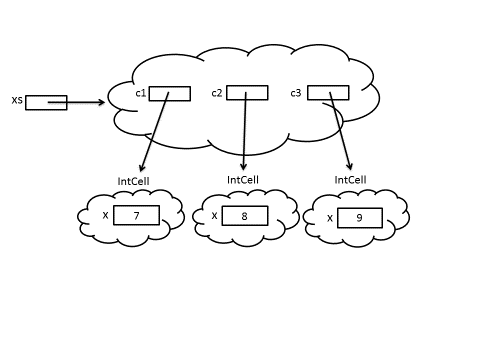
\includegraphics{../img/w05-solutions/memory-pic-1}

\SubtaskSolved  Istället för att skriva \code{IntCell(var x: Int)} så kan man skriva \code{IntCell(val x: Int)} där varje cells intvärde kommer vara oförändlig.
Alltså då attributen till objekten är “Val” så kommer även de att vara oförändliga.



\QUESTEND




%%<AUTOEXTRACTED by mergesolu>%%      % Uppgift 2




\WHAT{NEEDS A TOPIC DESCRIPTION}

\QUESTBEGIN

\Task  \what~ Föränderliga, indexerbara sekvenser: \code{Array} och \code{ArrayBuffer}

\Subtask Samlingen \code{scala.Array} har speciellt stöd i JVM och är extra snabb att allokera och indexera i. Dock kan man inte ändra storleken efter att en Array allokerats. Behöver man mer plats kan man kopiera den till en ny, större array. Koden nedan visar hur det kan gå till.
\begin{REPL}
scala> val xs = Array(42, 43, 44)
scala> val ys = new Array[Int](4)  //plats för 4 heltal, från början nollor
scala> for (i <- 0 until xs.size){ys(i) = xs(i)}
scala> ys(3) = 45
\end{REPL}
Definiera funktionen \code{def copyAppend(xs: Array[Int], x: Int): Array[Int]} som implementerar nedan algoritm, \emph{efter} att du rätta de \textbf{\color{red}{två buggarna}} i algoritmens while-loop:

\begin{algorithm}[H]
 \SetKwInOut{Input}{Indata}\SetKwInOut{Output}{Resultat}

 \Input{Heltalsarray $xs$ och heltalet $x$}
 \Output{En ny array som som är en kopia av $xs$ men med $x$ tillagt på slutet som extra element.}
 $n \leftarrow$ antalet element i $xs$ \\
 $ys \leftarrow$ en ny array med plats för $n + 1$ element\\
 $i \leftarrow 0$  \\
 \While{$i \leq n$}{
  $ys(i) \leftarrow xs(i)$
 }
 $ys(n) \leftarrow x$
\end{algorithm}



\Subtask Samlingen \code{scala.collection.mutable.ArrayBuffer} är inte riktigt lika snabb i alla lägen som \code{scala.Array} men storleksändring hanteras automatiskt, vilket är en stor fördel då man slipper att själv implementera algoritmer liknande \code{copyAppend} ovan. Speciellt använder man ofta \code{ArrayBuffer} om man stegvis vill bygga upp en sekvens. Vad händer nedan?
\begin{REPL}
scala> val xs = scala.collection.mutable.ArrayBuffer.empty[Int]
scala> xs.append(1, 1)
scala> while (xs.last < 100) {xs.append(xs.takeRight(2).sum); println(xs)}
scala> xs.last
scala> xs.length
\end{REPL}

\Subtask Talen i sekvensen som produceras ovan kallas Fibonaccital\footnote{\href{https://sv.wikipedia.org/wiki/Fibonaccital}{sv.wikipedia.org/wiki/Fibonaccital}}. Hur lång ska en Fibonacci-sekvens vara för att det sista elementet ska komma så nära (men inte över) \code{Int.MaxValue} som möjligt?



\SOLUTION


\TaskSolved \what


\SubtaskSolved  \begin{Code}
def copyAppend(xs: Array[Int], x: Int): Array[Int] = {
  val n = xs.size
  val ys = new Array[Int](n+1)
  var i = 0
  while(i < n) {
    ys(i) = xs(i)
    i += 1
  }
  ys(n) = x
  ys
}
\end{Code}

\SubtaskSolved  \begin{REPL}
xs: scala.collection.mutable.ArrayBuffer[Int] = ArrayBuffer()
ArrayBuffer(1, 1, 2)
ArrayBuffer(1, 1, 2, 3)
ArrayBuffer(1, 1, 2, 3, 5)
ArrayBuffer(1, 1, 2, 3, 5, 8)
ArrayBuffer(1, 1, 2, 3, 5, 8, 13)
ArrayBuffer(1, 1, 2, 3, 5, 8, 13, 21)
ArrayBuffer(1, 1, 2, 3, 5, 8, 13, 21, 34)
ArrayBuffer(1, 1, 2, 3, 5, 8, 13, 21, 34, 55)
ArrayBuffer(1, 1, 2, 3, 5, 8, 13, 21, 34, 55, 89)
ArrayBuffer(1, 1, 2, 3, 5, 8, 13, 21, 34, 55, 89, 144)
Int = 144
Int = 12
\end{REPL}

\SubtaskSolved  \code{xs.size = 46}\\
\code{xs(45) = 1836311903}\\
(Ha en arrayBuffer av typen Long istället och byt 100 mot Int.MaxValue och ta det nästsista elementet i sekvensens (det sista kommer vara över))


\QUESTEND




%%<AUTOEXTRACTED by mergesolu>%%      % Uppgift 3




\WHAT{Kopiering och uppdatering.}

\QUESTBEGIN

\Task  \what~  Metoder på oföränderliga samlingar skapar nya samlingar istället för att ändra. Därför behöver man inte själv skapa kopior. När en \emph{föränderlig} samling uppdateras på plats, syns denna förändring via alla referenser till samlingen.

\begin{REPL}
scala> val xs = Vector(1, 2, 3)
scala> val ys = xs.toArray
scala> ys(1) = 42
scala> xs
scala> ys
scala> val zs = ys.toArray
scala> zs(1) = 84
scala> xs
scala> ys
scala> zs
\end{REPL}

\Subtask Syns uppdateringen av objektet som \code{ys} refererar till via referensen \code{xs}? Varför?

\Subtask Syns uppdateringen av objektet som \code{zs} refererar till via referensen \code{ys}? Varför?

\Subtask Syns uppdateringen av objektet som \code{zs} refererar till via referensen \code{xs}? Varför?

\SOLUTION


\TaskSolved \what


\SubtaskSolved  Nej det gör det inte.
Då ys tilldelas xs.toArray kopieras datan från xs över i en array (som är mutable) vilket är en annan referens än den till xs.
Detta innebär att xs och ys inte “pekar” på samma objekt längre.

\SubtaskSolved  Ja därför båda är array och nu kopieras referensen till ys över till zs.
Därför kommer alla ändringar i zs att påverka ys (så länge de pekar på samma referens).

\SubtaskSolved  Nej det gör det inte. Se a).



\QUESTEND




%%<AUTOEXTRACTED by mergesolu>%%      % Uppgift 4




\WHAT{Färdig metod för att skapa kopia av array.}

\QUESTBEGIN

\Task  \what~  Om man inte vill att en uppdatering av en föränderlig samling ska få oönskad påverkan på andra koddelar som refererar till samlingen, behöver man göra kopior av samlingen före uppdatering. Det finns färdiga metoder för kopiering av objekt av typen Array i paketet \code{java.util.Arrays}.

\Subtask\Pen Studera dokumentationen för metoden \code{java.util.Arrays.copyOf} här:\\ \href{https://docs.oracle.com/javase/8/docs/api/java/util/Arrays.html\#copyOf-int:A-int-}{docs.oracle.com/javase/8/docs/api/java/util/Arrays.html\#copyOf-int:A-int-} \\
Notera att syntaxen för arrayer i Java är annorlunda: När det står \code{int[]} i Java så motsvarar det \code{Array[Int]} i Scala. Vad används den andra parametern till?

\Subtask\Pen Rita en bild av hur minnet ser ut efter varje tilldelning nedan. Vad har \code{xs}, \code{ys} och \code{zs} för värden efter exekveringen av raderna 1--5 nedan? Varför?
\begin{REPL}
scala> val xs = Array(1, 2, 3, 4)
scala> val ys = xs
scala> val zs = java.util.Arrays.copyOf(xs, xs.size - 1)
sxala> xs(0) = 42
scala> zs(0) = 84
scala> xs
scala> ys
scala> zs
\end{REPL}

\SOLUTION


\TaskSolved \what


\SubtaskSolved  Den andra parametern anger hur stor den nya vektorn som returneras ska vara.

\SubtaskSolved  \begin{enumerate}
\item 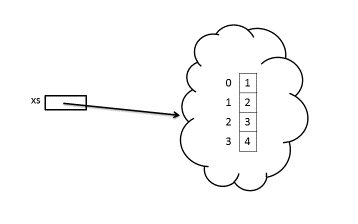
\includegraphics[scale=1.2]{../img/w05-solutions/memory-pic-2}
\item 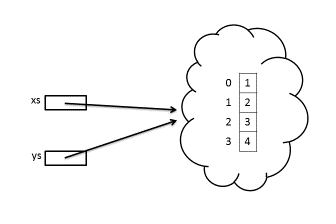
\includegraphics[scale=1.2]{../img/w05-solutions/memory-pic-3}
\item 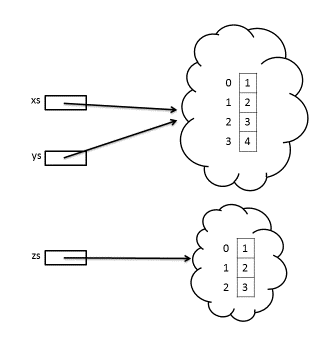
\includegraphics[scale=1.2]{../img/w05-solutions/memory-pic-4}
\item 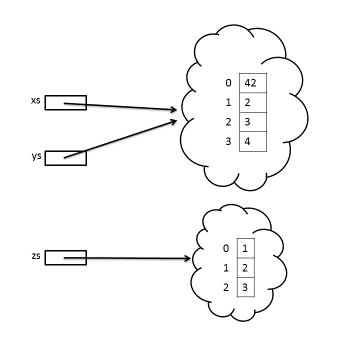
\includegraphics[scale=1.2]{../img/w05-solutions/memory-pic-5}
\item 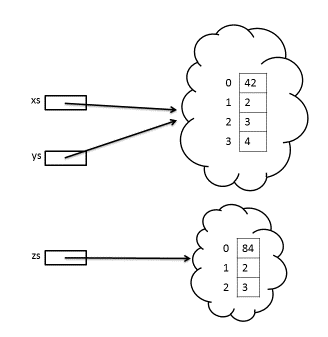
\includegraphics[scale=1.2]{../img/w05-solutions/memory-pic-6}
\end{enumerate}
xs = Array(42, 2, 3, 4)\\
ys = Array(42, 2, 3 ,4)\\
zs = Array(84, 2, 3)\\
\code{xs} och \code{yx} refererar till samma objekt och då deras första IntCell:s värde ändras till 42, så kommer förändringen att ske för båda.
\code{zs} har en referens till ett annat objekt med ett mindre element. Att \code{zs}:s första element ändras, påverkar inte \code{xs} och \code{ys}.



\QUESTEND




%%<AUTOEXTRACTED by mergesolu>%%      % Uppgift 5




\WHAT{Algoritm: SEQ-REVERSE-COPY.}

\QUESTBEGIN

\Task  \what~  Implementera nedan algoritm:

\begin{algorithm}[H]
 \SetKwInOut{Input}{Indata}\SetKwInOut{Output}{Resultat}

 \Input{Heltalsarray $xs$}
 \Output{En ny heltalsarray med elementen i $xs$ i omvänd ordning.}
 $n \leftarrow$ antalet element i $xs$ \\
 $ys \leftarrow$ en ny heltalsarray med plats för $n$ element\\
 $i \leftarrow 0$  \\
 \While{$i < n$}{
  $ys(n - i - 1) \leftarrow xs(i)$ \\
  $i \leftarrow i + 1$
 }
 \Return $ys$
\end{algorithm}

\Subtask\Pen Skriv implementation med penna och papper. Använd en \code{while}-sats på samma sätt som i algoritmen. Prova sedan din implementation på dator och kolla så att den fungerar.

\Subtask\Pen \label{subtask:for-seq-copy} Skriv implementationen med penna och papper igen, men använd nu istället en \code{for}-sats som räknar baklänges. Prova sedan din implementation på dator och kolla så att den fungerar.

\Subtask Definiera en funktion i REPL med namnet \code{reverseCopy} med din implementation i uppgift \ref{subtask:for-seq-copy}.


\SOLUTION


\TaskSolved \what


\SubtaskSolved  \begin{Code}
def seqReverseCopy(xs: Array[Int]): Array[Int] = {
  val n = xs.size
  val ys = Array.fill[Int](n)(0)
  var i = 0
  while(i < n) {
    ys(n-i-1) = xs(i)
    i += 1
  }
  ys
}
\end{Code}

\SubtaskSolved  \begin{Code}
def seqReverseCopy(xs: Array[Int]): Array[Int] = {
  val n = xs.size
  val ys = Array.fill[Int](n)(0)
  for(i <- n-1 to 0 by -1) ys(n-i-1) = xs(i)
  ys
}
\end{Code}

\SubtaskSolved  Se b).



\QUESTEND




%%<AUTOEXTRACTED by mergesolu>%%      % Uppgift 6




\WHAT{Algoritm: SEQ-REVERSE.}

\QUESTBEGIN

\Task  \what~  Strängar av typen \code{String} är oföränderliga. Vill man ändra i en sträng utan att skapa en ny kopia kan man använda en \code{StringBuilder} enligt nedan algoritm som vänder bak-och-fram på en sträng.

\begin{algorithm}[H]
 \SetKwInOut{Input}{Indata}\SetKwInOut{Output}{Resultat}

 \Input{En sträng $s$ av typen \texttt{String}}
 \Output{En ny sträng av typen \texttt{String}}
 $sb \leftarrow$ en ny \texttt{StringBuilder} som innehåller $s$ \\
 $n \leftarrow$ antalet tecken i $s$\\
 \For{$i \leftarrow 0$ \KwTo $\frac{n}{2} - 1$}{
  $temp \leftarrow sb(i)$ \\
  $sb(i) \leftarrow sb(n - i - 1)$ \\
  $sb(n - i - 1) \leftarrow temp$ \\
 }
 \Return $sb$ omvandlad till en \texttt{String}
\end{algorithm}

\Subtask Implementera algoritmen ovan i en funktion med signaturen: \\
 \code{def reverseString(s: String): String}

\Subtask Använd din funktion \code{reverseString} från föregående deluppgift i en ny funktion med signaturen:\\
 \code{def isPalindrome(s: String): Boolean} \\ som avgör om en sträng är en palindrom.\footnote{\href{https://sv.wikipedia.org/wiki/Palindrom}{sv.wikipedia.org/wiki/Palindrom}}

\Subtask\Pen Man kan med en \code{while}-sats och indexering direkt i en \code{String} avgöra om en sträng är en palindrom utan att kopiera den till en \code{StringBuilder}. Implementera en ny variant av \code{isPalindrome} som använder denna metod. Skriv först algoritmen på papper i pseudo-kod.

\SOLUTION


\TaskSolved \what


\SubtaskSolved  \begin{Code}
def reverseString(s: String): String = {
  val sb = new StringBuilder(s)
  val n = sb.length
  for (i <- 0 until n / 2) {
    val temp = sb(i)
    sb(i) = sb(n - i - 1)
    sb(n - i - 1) = temp
  }
  sb.toString
}
\end{Code}

\SubtaskSolved  \begin{Code}
def isPalindrome(s: String): Boolean = {s == reverseString(s)}
\end{Code}

\SubtaskSolved  \begin{Code}
def isPalindrome(s: String): Boolean = {
  val n = s.length
  var foundDiff = false
  var i = 0
  while (i < n/2 && !foundDiff)  {
    foundDiff = s(i) != s(n - i - 1)
    i += 1
  }
  !foundDiff
}
\end{Code}



\QUESTEND




%%<AUTOEXTRACTED by mergesolu>%%      % Uppgift 7




\WHAT{Algoritm: SEQ-REGISTER.}

\QUESTBEGIN

\Task \label{task:seq-reg} \what~   Algoritmer för registrering löser problemet att räkna förekomst av olika saker, till exempel antalet tärningskast som gav en sexa. Antag att vi har följande vektor \code{xs} som representerar 13 st tärningskast:
\begin{REPL}
scala> val xs = Vector(5, 3, 1, 6, 1, 3, 5, 1, 1, 6, 3, 2, 6)
\end{REPL}
\Subtask Använd metoderna \code{filter} och \code{size} på \code{xs} för att filtrera ut alla 6:or och räkna hur många de är.

\Subtask Använd metoderna \code{filter} och \code{size} på \code{xs} för att filtrera ut alla jämna kast och räkna hur många de är.

\Subtask Metoden \code{groupBy} på en samling tar en funktion \code{f} som parameter och skapar en ny \code{Map} med nycklar \code{k} som är associerade till samlingar som utgör grupper av värden där
\code{f(x) == k}.  Vad händer här:
\begin{REPL}
scala> xs.groupBy(x => x % 2)
scala> xs.groupBy(_ % 2)
scala> xs.groupBy(_ % 3)
scala> xs.groupBy(_ % 3).foreach(println)
scala> val freqEvenOdd = xs.groupBy(_ % 2).map(p => (p._1, p._2.size))
scala> val nEven = freqEvenOdd(0)
scala> val nOdd = freqEvenOdd(1)
\end{REPL}
\Subtask Använd metoden \code{groupBy} på \code{xs} med den s.k. identitetsfunktionen \code{i => i} som returnerar sitt eget argument. Vad händer?

\Subtask Definiera en \code{val freq: Map[Int, Int]} som räknar antalet olika tärningsutfall i \code{xs}. Använd metoden \code{groupBy} på \code{xs} med identitetsfunktionen följt av en \code{map} med funktionen \code{p => (p._1, p._2.size)}.

\Subtask Du ska nu själv implementera en registreringsalgoritm. Skriv en funktion:
\begin{Code}
def tärningsRegistrering(xs: Array[Int]): Array[Int] = ???
\end{Code}
som implementerar nedan algoritm (som alltså inte använder \code{groupBy} eller andra färdiga metoder på samlingar förutom \code{size} och \code{apply}).

\begin{algorithm}[H]
 \SetKwInOut{Input}{Indata}\SetKwInOut{Output}{Resultat}

 \Input{En array $xs$ med heltal mellan 1 och 6 som representerar utfall av många tärningskast.}
 \Output{En array $f$ med 7 st element där $f(0)$ innehåller totala antalet kast, $f(1)$ anger antalet ettor, $f(2)$ antalet tvåor, etc. till och med $f(6)$ som anger antalet sexor.}
 $f \leftarrow$ en ny array med $7$ element där alla element initaliseras till 0.\\
 $f(0) \leftarrow$ antalet element i $xs$ \\
 $i \leftarrow 0$  \\
 \While{$i < f(0)$}{
  $f(xs(i)) \leftarrow f(xs(i)) + 1$ \\
  $i \leftarrow i + 1$
 }
 \Return $f$
\end{algorithm}

Testa din funktion med nedan funktionsanrop:
\begin{REPL}
scala> tärningsRegistrering(Array.fill(1000)((math.random * 6).toInt + 1))
res12: Array[Int] = Array(1000, 174, 174, 167, 171, 145, 169)
\end{REPL}

\SOLUTION


\TaskSolved \what


\SubtaskSolved  \code{xs.filter(_ == 6).size}

\SubtaskSolved  \code{xs.filter(_ % 2 == 0).size}

\SubtaskSolved  \begin{REPL}
scala.collection.immutable.Map[Int,scala.collection.immutable.Vector[Int]] =
	Map(1 -> Vector(5, 3, 1, 1, 3, 5, 1, 1, 3), 0 -> Vector(6, 6, 2, 6))
scala.collection.immutable.Map[Int,scala.collection.immutable.Vector[Int]] =
	Map(1 -> Vector(5, 3, 1, 1, 3, 5, 1, 1, 3), 0 -> Vector(6, 6, 2, 6))
scala.collection.immutable.Map[Int,scala.collection.immutable.Vector[Int]] =
	Map(2 -> Vector(5, 5, 2), 1 -> Vector(1, 1, 1, 1), 0 -> Vector(3, 6, 3, 6, 3, 6))
(2,Vector(5, 5, 2))
(1,Vector(1, 1, 1, 1))
(0,Vector(3, 6, 3, 6, 3, 6))
freqEvenOdd: scala.collection.immutable.Map[Int,Int] = Map(1 -> 9, 0 -> 4)
nEven: Int = 4
nOdd: Int = 9
\end{REPL}

\SubtaskSolved  \code{xs.groupBy(i => i)} skapar en map där nycklarna är alla unika element och värdena är av samma värde som respektive nyckel.

\SubtaskSolved  \code{val freq: Map[Int, Int] = xs.groupBy(i => i).map(p => (p._1, p._2.size))}

\SubtaskSolved  \begin{Code}
def tärningsRegistrering(xs: Array[Int]): Array[Int] = {
  val f = Array.fill(7)(0)
  f(0) = xs.size
  var i = 0
  while (i < f(0)) {
    f(xs(i)) += 1
    i += 1
  }
  f
}
\end{Code}



\QUESTEND




%%<AUTOEXTRACTED by mergesolu>%%      % Uppgift 8




\WHAT{Algoritm: SEQ-REMOVE-COPY.}

\QUESTBEGIN

\Task  \what~  Ibland vill man kopiera alla element till en ny \code{Array} \emph{utom} ett element på en viss plats \code{pos}.

\Subtask\Pen Skriv algoritmen SEQ-REMOVE-COPY i pseudokod med penna på papper.

\Subtask Implementera algoritmen SEQ-REMOVE-COPY i en funktion med denna signatur:
\begin{Code}
def removeCopy(xs: Array[Int], pos: Int): Array[Int]
\end{Code}

\SOLUTION


\TaskSolved \what


\SubtaskSolved

\begin{algorithm}[H]
 \SetKwInOut{Input}{Indata}\SetKwInOut{Output}{Resultat}

 \Input{En sekvens $xs$ av typen \texttt{Array[Int]} och $pos$}
 \Output{En ny sekvens av typen \texttt{Array[Int]} som är en kopia av $xs$ fast med elementet på plats $pos$ borttaget}
 $n \leftarrow$ antalet element $xs$\\
 $ys \leftarrow$ en ny \texttt{Array[Int]} med plats för $n-1$ element \\
 \For{$i \leftarrow 0$ \KwTo $pos - 1$}{
  $ys(i) \leftarrow xs(i)$
 }
 $ys(pos) \leftarrow x$ \\
 \For{$i \leftarrow pos+1$ \KwTo $n - 1$}{
  $ys(i - 1) \leftarrow xs(i)$
 }
 \Return $ys$
\end{algorithm}

\SubtaskSolved  \begin{Code}
def removeCopy(xs: Array[Int], pos: Int): Array[Int] = {
  val n = xs.size
  val ys = Array.fill(n - 1)(0)
  for (i <- 0 until pos) ys(i) = xs(i)
  for (i <- pos+1 until n) ys(i - 1) = xs(i)
  ys
}
\end{Code}



\QUESTEND




%%<AUTOEXTRACTED by mergesolu>%%      % Uppgift 9




\WHAT{Algoritm: SEQ-REMOVE.}

\QUESTBEGIN

\Task  \what~  Ibland vill man ta bort ett element på en viss position i en befintlig \code{Array} utan att kopiera alla element till en ny \code{Array}. Ett sätt att göra detta är att flytta alla efterföljande element ett steg mot lägre index och låta sista platsen bli 0.

\Subtask\Pen Skriv algoritmen SEQ-REMOVE i pseudokod med penna på papper.

\Subtask Implementera algoritmen SEQ-REMOVE i en funktion med denna signatur:
\begin{Code}
def remove(xs: Array[Int], pos: Int): Unit
\end{Code}


%%%%%%%%%%%%%%%%%%%%%%%%%%%%%%%%%%%%%%%%%%%5


\SOLUTION


\TaskSolved \what


\SubtaskSolved

\begin{algorithm}[H]
 \SetKwInOut{Input}{Indata}\SetKwInOut{Output}{Resultat}

 \Input{En sekvens $xs$ av typen \texttt{Array[Int]} och $pos$}
 \Output{En uppdaterad sekvens av $xs$ där elementet på plats $pos$ tagits bort och efterföljande element flyttas ett steg mot lägre index med ett sista elementet som är $0$}
 $n \leftarrow$ antalet element $xs$\\
 \For{$i \leftarrow pos+1$ \KwTo $n - 1$}{
  $xs(i - 1) \leftarrow xs(i)$
 }
 $xs(n - 1) \leftarrow 0$ \\
\end{algorithm}

\SubtaskSolved  \begin{Code}
def remove(xs: Array[Int], pos: Int): Unit = {
  val n = xs.size
  for (i <- pos+1 until n) xs(i - 1) = xs(i)
  xs(n-1) = 0
}
\end{Code}



\QUESTEND




%%<AUTOEXTRACTED by mergesolu>%%      % Uppgift 10




\WHAT{Deterministiska pseudoslumptalssekvenser med \code{java.util.Random}.}

\QUESTBEGIN

\Task  \what~  Klassen \code{java.util.Random} ger möjlighet att generera en sekvens av tal som verkar slumpmässiga. Genom att välja ett visst s.k. \textbf{frö} \Eng{seed} kan man få samma sekvens av pseudoslumptal varje gång.

\Subtask\Pen Sök upp och studera dokumentationen för \code{java.util.Random}. Hur skapar man en ny instans av klassen \code{Random}? Vad gör operationen \code{nextInt} på \code{Random}-objekt.

\Subtask Förklara vad som händer nedan?
\begin{REPL}
scala> import java.util.Random
scala> val frö = 42L
scala> val rnd = new Random(frö)
scala> rnd.nextInt(10)
scala> (1 to 100).foreach(_ => print(rnd.nextInt(10)))
scala> val rnd1 = new Random(frö)
scala> val rnd2 = new Random(frö)
scala> val rnd3 = new Random(System.nanoTime)
scala> val rnd4 = new Random((math.random * Long.MaxValue).toLong)
scala> def flip(r: Random) = if (r.nextInt(2) > 0) "krona" else "klave"
scala> val xs = (1 to 100).map{i =>
			(flip(rnd1), flip(rnd2), flip(rnd3), flip(rnd4))}
scala> xs foreach println
scala> xs.exists(q => q._1 != q._2)
scala> xs.exists(q => q._1 != q._3)
\end{REPL}

\Subtask\Pen Nämn några sammanhang då det är användbart att kunna bestämma fröet till en slumptalssekvens.

\Subtask Blir det samma sekvens om du använder fröet \code{42L} som argument till konstruktorn vid skapandet av en instans av \code{java.util.Random} på en \emph{annan} dator?

\Subtask Sök reda på dokumentationen för \code{java.math.random} och undersök hur denna sekvens skapas.

\Subtask Vad blir det för frö till slumptalssekvensen om man skapar ett \code{Random}-objekt med hjälp av konstruktorn utan parameter?

\SOLUTION


\TaskSolved \what


\SubtaskSolved  Antingen kan du skapa en ny instans av \code{java.util.Random} genom att skriva: \code{val r1 = new java.util.Random}.
Men om \code{java.util.Random} importeras kan “java.util” skippas och istället skrivs: \code{val r2 = new Random}.
Som valfritt argument kan ett slumptalsfrö av typen Long skickas med när en ny instans skapas, e.g. \code{val r3 = new Random(42L)}.
\code{nextInt(x)} skapar ett slumptal från och med 0, upp till x (exklusive x).

\SubtaskSolved  \begin{REPL}
import java.util.Random // Importerar Random

frö: Long = 42 // Ett slumptalsfrö av värdet 42L skapas.

  // Skapar ett Random objekt med slumptalsfrö "frö".
rnd: java.util.Random = java.util.Random@2f410acf

res0: Int = 7 // Slumpade fram ett tal från 0 till och med 9.

9 8 8 8 9 7 2 1 4 0 0 3 8 8 4 5 9 1 3 3 5 1 1
3 3 3 6 3 4 7 5 7 8 7 6 9 7 0 3 0 6 6 1 0 8 1
1 1 0 5 3 5 1 5 3 5 9 9 5 1 8 9 0 6 4 7 5 7 9
6 4 0 8 1 0 9 6 6 3 2 7 9 2 7 0 6 9 8 5 0 0 8
9 2 7 7 3 5 1 3 // Slumpar och skriver ut 100 tal från 0 till och med 9.

  // Skapar ett Random objekt med slumptalsfrö "frö".
rnd1: java.util.Random = java.util.Random@31e4bb20

  // Skapar ett Random objekt med slumptalsfrö "frö".
rnd2: java.util.Random = java.util.Random@45e37a7e

  // Skapar ett Random objekt med slumptalsfrö med
  // värdet av vad tiden är just nu i nanosekunder.
rnd3: java.util.Random = java.util.Random@57eda880

  // Skapar ett Random objekt med slumptalsfrö
  // med värdet (math.random * Long.MaxValue).toLong.
rnd4: java.util.Random = java.util.Random@79da1ec0

flip: (r: java.util.Random)String // Skapar en funktion som singlar slant.

  // Singlar slant med alla fyra Random
  // objekt 100 gånger samt printar ut resultatet.
xs: scala.collection.immutable.IndexedSeq[(String, String, String, String)] =
Vector((krona,krona,krona,klave), (klave,klave,krona,krona), (krona,krona,klave,klave),
(klave,klave,krona,klave), (klave,klave,krona,krona), (krona,krona,klave,krona),
(klave,klave,klave,klave), (krona,krona,klave,krona), (krona,krona,klave,krona),
(klave,klave,krona,klave), (krona,krona,krona,klave), (klave,klave,krona,klave),
(klave,klave,krona,krona), (klave,klave,klave,krona), (klave,klave,klave,krona),
(krona,krona,klave,klave), (klave,klave,klave,klave), (krona,krona,klave,krona),
(krona,krona,klave,klave), (krona,krona,klave,klave), (krona,krona,klave,krona),
(klave,klave,klave,klave), (klave,klave,krona,krona), (klave,klave,klave,klave),
(krona,krona,krona,krona), (krona,krona,krona,klave)...

  // Kollar om det finns något värde som rnd1
  // har genererat men som inte rnd2 genererat.
res1: Boolean = false

  // Kollar om det finns något värde som rnd1
  // har genererat men som inte rnd3 genererat.
res2: Boolean = true

\end{REPL}

\SubtaskSolved  Vid felsökning och vid simulering där man vill att samma “slumpmässiga” sekvens uppstår varenda gång.

\SubtaskSolved  Ja.

\SubtaskSolved  \url{https://docs.oracle.com/javase/7/docs/api/java/lang/Math.html#random%28%29--} säger att den skapar ett nytt java.util.Random-objekt.

\SubtaskSolved  Den skapar ett slumpmässigt slumptalsfrö. För mer information, se: \url{https://docs.oracle.com/javase/8/docs/api/java/util/Random.html#Random--}



\QUESTEND




%%<AUTOEXTRACTED by mergesolu>%%      % Uppgift 11




\WHAT{Undersök om tärningskast är rektangelfördelade.}

\QUESTBEGIN

\Task  \what~ \footnote{För ett rektangelfördelat slumpvärde gäller att om man drar (nästan oändligt många) slumpvärden så blir det (nästan) lika många av varje möjligt värde. Om man ritar en sådan fördelning i ett koordinatsystem med antalet utfall på y-axeln och de olika värdena på x-axeln, så blir bilden rektangelformad. Du får lära dig mer om sannolikhetsfördelningar i kommande kurser i matematisk statistik.} \\Skriv en funktion \code{def testRandom(r: Random, n: Int): Unit = ???} \\ som ger följande utskrift:
\begin{REPL}
scala> val rnd = new Random(42L)
scala> testRandom(rnd, 1000)
Antal kast: 1000
Antal 1:or: 178
Antal 2:or: 187
Antal 3:or: 167
Antal 4:or: 148
Antal 5:or: 155
Antal 6:or: 165
\end{REPL}

\emph{Tips:}
Anropa din funktion \code{tärningsRegistrering} från uppgift \ref{task:seq-reg}.


\SOLUTION


\TaskSolved \what


\begin{Code}
def testRandom(r: Random, n: Int): Unit = {
  val xs = Array.fill(n)(r.nextInt(6) + 1)
  val f = tärningsRegistrering(xs)
  println("Antal kast: " + f(0))
  for (i <- 1 to 6) println(s"Antal $i:or: " + f(i))
}
\end{Code}



\QUESTEND




%%<AUTOEXTRACTED by mergesolu>%%      % Uppgift 12




\WHAT{Array och \code{for}-sats i Java.}

\QUESTBEGIN

\Task  \what~

\Subtask Skriv nedan program i en editor och spara i filen \code{DiceReg.java}:

\javainputlisting{examples/DiceReg.java}

\Subtask Kompilera med \code{javac DiceReg.java} och kör med \code{java DiceReg 10000 42} och förklara vad som händer.

\Subtask\Pen Beskriv skillnaderna mellan Scala och Java, vad gäller syntaxen för array och \code{for}-sats. Beskriv några andra skillnader mellan språken som syns i programmet ovan.

\Subtask Ändra i programmet ovan så att loop-variabeln \code{i} skrivs ut i varje runda i varje \code{for}-sats. Kompilera om och kör.

\Subtask Skriv om programmet ovan genom att abstrahera huvudprogrammets delar till de statiska metoderna \code{parseArguments}, \code{registerPips} och \code{printReg} enligt nedan skelett. Notera speciellt hur \jcode{private} och \jcode{public} är angivet. Spara programmet i filen \code{DiceReg2.java} och kompilera med \texttt{javac DiceReg2.java} i terminalen.

\begin{Code}[language=Java]
// DiceReg2.java
import java.util.Random;

public class DiceReg2 {
    public static int[] diceReg = new int[6];
    private static Random rnd = new Random();

    public static int parseArguments(String[] args) {
        // ???
        return n;
    }

    public static void registerPips(int n){
        // ???
    }

    public static void printReg() {
        // ???
    }

    public static void main(String[] args) {
        int n = parseArguments(args);
        registerPips(n);
        printReg();
    }
}
\end{Code}

\Subtask Starta Scala REPL i samma bibliotek som filen \texttt{DiceReg2.class} ligger i och kör nedan satser och förklara vad som händer:
\begin{REPL}
scala> DiceReg2.main(Array("1000","42"))
scala> DiceReg2.diceReg
scala> DiceReg2.registerPips(1000)
scala> DiceReg2.printReg
scala> DiceReg2.registerPips(1000)
scala> DiceReg2.printReg
scala> DiceReg2.rnd
\end{REPL}

\Subtask Växla synligheten på attributen mellan \jcode{private} och \jcode{public}, kompilera om och studera effekten i Scala REPL. Hur lyder felmeddelandet om du försöker komma åt en privat medlem?

\Subtask\Pen Ange en viktig anledning till att man kan vilja göra medlemmar privata.



\SOLUTION


\TaskSolved \what


\SubtaskSolved  -

\SubtaskSolved  \begin{REPL}
Rolling the dice 10000 times with seed 42
Number of 1's: 1654
Number of 2's: 1715
Number of 3's: 1677
Number of 4's: 1629
Number of 5's: 1643
Number of 6's: 1682
\end{REPL}
Simulerar 10000 tärningskast (med slumptalsfrö 42) och skriver ut förekomsten av respektive tärningskast.

\SubtaskSolved  Array i scala deklararas: \code{val scalaArray = Array.ofDim[Int](6)} medan i java skrivs: \code{int[] javaArray = new int[6];}
\code{for}-sats i scala skrivs: \code{for(i <- 0 to n)} medan i java skrivs: \code{for (int i = 0; i < n; i++)}.
I java måste semicolon skrivas efter varje operation samt att typen måste explicit definieras vid variabeldeklaration.
I scala behövs inga semicolon (förutom för att separera operationer på samma rad) och scala bestäms typen implicit, alltså att kompilatorn “gissar” typen av variabeln som deklareras.

\SubtaskSolved  Lägg till \code{System.out.println(i);} i for-looparna

\SubtaskSolved  \begin{Code}[language=Java]
// DiceReg2.java
import java.util.Random;
public class DiceReg2{
	public static int[] diceReg = new int[6];
	private static Random rnd = new Random();

	public static int parseArguments(String[] args){
		int n = 100;
		if(args.length > 0) {
			n = Integer.parseInt(args[0]);
		}
		if(args.length > 1) {
			int seed = Integer.parseInt(args[1]);
			rnd.setSeed(seed);
		}
		return n;
	}

	public static void registerPips(int n) {
		for(int i = 0; i<n; i++) {
			int pips = rnd.nextInt(6);
			diceReg[pips]++;
		}
	}

	public static void main(String[] args) {
		int n = parseArguments(args);
		registerPips(n);
		printReg();
	}
}
\end{Code}

\SubtaskSolved  \begin{REPL}
  // Skriver ut förekomsten av 1000 tärningskast med slumptalsfrö 42.
Number of 1's: 165
Number of 2's: 163
Number of 3's: 178
Number of 4's: 183
Number of 5's: 156
Number of 6's: 155

  // Skriver ut diceReg-attributet
res1: Array[Int] = Array(165, 163, 178, 183, 156, 155)

  // Skriver ut diceReg-attributet efter 1000 till kast.
res2: Array[Int] = Array(329, 325, 349, 360, 324, 313)

  // Skriver ut diceReg-attributet efter 1000 till kast.
res3: Array[Int] = Array(498, 484, 531, 513, 485, 489)

  // Det blir runtime error då attributet rnd är
  // private och kan inte nås via REPL:n.
<console>:11: error: value rnd is not a member of object DiceReg2
	DiceReg2.rnd
				    ^
\end{REPL}

\SubtaskSolved  \begin{REPL}
value [diceReg/rnd] is not a member of object DiceReg2
\end{REPL}

\SubtaskSolved  Om man ska spara under någon data som man inte vill att användaren, eller någon annan, inte ska kunna komma åt.
T.ex. om du gör en bankapp vill du inte att nyckeln som du använder för att autorisera en användare ska vara tillgänglig för då kan hackare använda det för att ta sig in på kontot och stjäla pengar!



\QUESTEND




%%<AUTOEXTRACTED by mergesolu>%%      % Uppgift 13




\WHAT{Läsa in tal med \code{java.util.Scanner}.}

\QUESTBEGIN

\Task  \what~  Med \jcode{new Scanner(System.in)} skapas ett objekt som kan läsa in tal som användaren skriver i terminalfönstret.

\Subtask Sök upp och studera dokumentationen för \code{java.util.Scanner}. Vad gör metoderna \jcode{hasNextInt()} och \jcode{nextInt()}?

\Subtask Skriv nedan program i en editor och spara i filen \code{DiceScanBuggy.java}:

\javainputlisting{examples/DiceScanBuggy.java}

\Subtask Kompilera och kör med indatasekvensen \texttt{1 2 3 4 -1} och notera hur registreringen sker.

\Subtask Programmet fungerar inte som det ska. Du behöver korrigera 3 saker för att programmet ska göra rätt. Rätta buggarna och spara det rättade programmet som \texttt{DiceScan.java}. Kompilera och testa att det rättade programmet fungerar med olika indata.


\SOLUTION


\TaskSolved \what


\SubtaskSolved  \code{hasNextInt()} kollar enbart om det finns ett till tal och returnerar \code{true}/\code{false}. \code{nextInt()} “hoppar” till nästa tal och returnerar det.
Se \url{https://docs.oracle.com/javase/7/docs/api/java/util/Scanner.html#hasNextInt%28%29} och \url{https://docs.oracle.com/javase/7/docs/api/java/util/Scanner.html#nextInt%28%29 }.

\SubtaskSolved  -

\SubtaskSolved  -

\SubtaskSolved  \begin{Code}[language=Java,numbers=left]
import java.util.Random;
import java.util.Scanner;

public class DiceScanBuggy {
	public static int[] diceReg = new int[6];
	public static Scanner scan = new Scanner(System.in);

	public static void registerPips() {
		System.out.println("Enter pips separated by blanks: ");
		System.out.println("End with -1 and <Enter>.");
		boolean isPips = true;
		while(isPips && scan.hasNextInt()){
			int pips = scan.nextInt();
			if(pips >= 1 && pips <= 6) {
				diceReg[pips-1]++;
			} else {
				isPips = false;
			}
		}
	}

	public static void printReg(){
		for(int i = 1; i<7; i++) {
		System.out.println("Number of " + i + "'s: " + diceReg[i-1]);
		}
	}

	public static void main(String[] args) {
		registerPips();
		printReg();
	}
}
\end{Code}


\QUESTEND




%%<AUTOEXTRACTED by mergesolu>%%      % Uppgift 14




\WHAT{Välja sekvenssamling.}

\QUESTBEGIN

\Task  \what~\Pen  Vilken av \code{Vector}, \code{Array} och \code{ArrayBuffer} hade du valt i dessa situationer?

\Subtask Ditt program innehåller en sekvens av objekt med data om alla ca $10^7$ medborgare i Sverige. Efter noggranna mätningar visar det sig att tillägg av objekt på godtyckliga ställen i sekvensen är en flaskhals.

\Subtask Ditt program innehåller en sekvens av objekt med data om ca $10^2$ \href{https://sv.wikipedia.org/wiki/Residensstad#Sverige}{residensstäder} i Sverige. Senast det skedde en uppdatering av mängden referensstäder var 1997. Prestandamätningar visar att det är uppdatering av attributvärden i objekten som tar mest tid. Städerna behöver kunna bearbetas i godtycklig ordning.

\Subtask Ditt program innehåller en sekvens av ca $10^9$ osorterade heltal som ska läsas in från fil och sorteras på plats i minnet. Det första talet i filen anger antalet heltal. Det är viktigt att sorteringen går snabbt. När talen är sorterade ska de skrivas tillbaka till fil i sorterad ordning.

\Subtask Ditt program innehåller en sekvens av ett känt antal oföränderliga objekt med data om genomförda banktransaktioner. Sekvensen ska bearbetas parallellt i godtycklig ordning med olika algoritmer som kan köras oberoende av varandra.


\ExtraTasks %%%%%%%%%%%%%%%%%%%

\SOLUTION


\TaskSolved \what


\SubtaskSolved  \code{ArrayBuffer}.

\SubtaskSolved  \code{ArrayBuffer} eller \code{Array}.

\SubtaskSolved  \code{Array}.

\SubtaskSolved  \code{Vector}.



\ExtraTasks %%%%%%%%%%%%


\QUESTEND




%%<AUTOEXTRACTED by mergesolu>%%      % Uppgift 15




\WHAT{Algoritm: SEQ-INSERT-COPY.}

\QUESTBEGIN

\Task  \what~

\begin{algorithm}[H]
 \SetKwInOut{Input}{Indata}\SetKwInOut{Output}{Resultat}

 \Input{En sekvens $xs$ av typen \texttt{Array[Int]} och heltalen $x$ och $pos$}
 \Output{En ny sekvens av typen \texttt{Array[Int]} som är en kopia av $xs$ men där $x$ är infogat på plats $pos$}
 $n \leftarrow$ antalet element $xs$\\
 $ys \leftarrow$ en ny \texttt{Array[Int]} med plats för $n+1$ element \\
 \For{$i \leftarrow 0$ \KwTo $pos - 1$}{
  $ys(i) \leftarrow xs(i)$
 }
 $ys(pos) \leftarrow x$ \\
 \For{$i \leftarrow pos$ \KwTo $n - 1$}{
  $ys(i + 1) \leftarrow xs(i)$
 }
 \Return $ys$
\end{algorithm}

\Subtask Implementera ovan algoritm i en funktion med denna signatur:
\begin{Code}
def insertCopy(xs: Array[Int], x: Int, pos: Int): Array[Int]
\end{Code}

\Subtask Vad måste \code{pos} vara för att det ska fungera med en tom array som argument?

\Subtask Vad händer om din funktion anropas med ett negativt argument för \code{pos}?

\Subtask Vad händer om din funktion anropas med \code{pos} lika med \code{xs.size}?

\Subtask Vad händer om din funktion anropas med \code{pos} större än \code{xs.size}?



\SOLUTION


\TaskSolved \what


\SubtaskSolved  \begin{Code}
def insertCopy(xs: Array[Int], x: Int, pos: Int): Array[Int] = {
  val n = xs.size
  val ys = Array.ofDim[Int](n + 1)
  for (i <- 0 until pos) ys(i) = xs(i)
  ys(pos) = x
  for (i <- pos until n) ys(i + 1) = xs(i)
  ys
}
\end{Code}

\SubtaskSolved  \code{pos} måste vara \code{0}.

\SubtaskSolved  \begin{REPL}
java.lang.ArrayIndexOutOfBoundsException: -1
\end{REPL}

\SubtaskSolved  Elementet \code{x} läggs till på slutet av arrayen, alltså kommer den returnerande arrayen vara större än den som skickades in.

\SubtaskSolved  \begin{REPL}
java.lang.ArrayIndexOutOfBoundsException: 5
\end{REPL}
Man får \code{ArrayIndexOutOfBoundsException} då indexeringen är utanför storleken hos arrayen.


\QUESTEND




%%<AUTOEXTRACTED by mergesolu>%%      % Uppgift 16




\WHAT{Algoritm: SEQ-INSERT.}

\QUESTBEGIN

\Task  \what~  Man kan implementera algoritmen SEQ-INSERT på plats i en \code{Array[Int]} så att alla elementen efter \code{pos} flyttas fram ett steg och att sista elementet ''försvinner''.

\Subtask\Pen Skriv algoritmen SEQ-INSERT i pseudokod med penna och papper.

\Subtask Implemtera SEQ-INSERT i en funktion med denna signatur:
\begin{Code}
def insert(xs: Array[Int], x: Int, pos: Int): Unit
\end{Code}

\SOLUTION


\TaskSolved \what


\SubtaskSolved

\begin{algorithm}[H]
 \SetKwInOut{Input}{Indata}\SetKwInOut{Output}{Resultat}

 \Input{En sekvens $xs$ av typen \texttt{Array[Int]} och heltalen $x$ och $pos$}
 \Output{En uppdaterad sekvens av $xs$ där elementet $x$ har satts in på platsen $pos$ och efterföljande element flyttas ett steg där sista elementet försvinner}
 $n \leftarrow$ antalet element $xs$\\
 $ys \leftarrow$ en klon av $xs$\\
 $xs(pos) \leftarrow x$\\
 \For{$i \leftarrow pos+1$ \KwTo $n - 1$}{
  $xs(i) \leftarrow ys(i - 1)$
 }
\end{algorithm}

\SubtaskSolved  \begin{Code}
def insert(xs: Array[Int], x: Int, pos: Int): Unit = {
  val n = xs.size
  val ys = xs.clone
  xs(pos) = x
  for (i <- pos + 1 until n) xs(i) = ys(i - 1)
}
\end{Code}



\QUESTEND




%%<AUTOEXTRACTED by mergesolu>%%      % Uppgift 17




\WHAT{NEEDS A TOPIC DESCRIPTION}

\QUESTBEGIN

\Task  \what~ Implementera funktionen \code{tärningsRegistrering} från uppgift \ref{task:seq-reg} på nytt, men nu med en \code{for}-sats istället.


\SOLUTION


\TaskSolved \what


\begin{Code}
def tärningsRegistrering(xs: Array[Int]): Array[Int] = {
  val f = Array.fill(7)(0)
  f(0) = xs.size
  for(i <- 0 until f(0)) f(xs(i)) += 1
  f
}
\end{Code}



\QUESTEND




%%<AUTOEXTRACTED by mergesolu>%%      % Uppgift 18




\WHAT{NEEDS A TOPIC DESCRIPTION}

\QUESTBEGIN

\Task  \what~ Bygg vidare på Keno-uppgiften nummer \ref{task:keno-set} i kapitel \ref{chapter:W04} på sidan \pageref{task:keno-set} och gör registrering av det slumpmässiga utfallet av 365 Keno-dragningar och skriv ut frekvenserna för förekomsten av varje boll. Öka sedan antalet dragningar och undersök hur många dragningar du behöver göra för att frekvenserna ska bli nästan lika?


\AdvancedTasks %%%%%%%%%%%%%%%%%

\SOLUTION


\TaskSolved \what




\AdvancedTasks %%%%%%%%%



\QUESTEND




%%<AUTOEXTRACTED by mergesolu>%%      % Uppgift 19




\WHAT{NEEDS A TOPIC DESCRIPTION}

\QUESTBEGIN

\Task  \what~ Sök reda på dokumentationen för metoden \code{patch} på klassen \code{Array}.

\Subtask Använd metoden \code{patch} för att implementera SEQ-INSERT-COPY:
\begin{Code}
def insertCopy(xs: Array[Int], x: Int, pos: Int): Array[Int] =
  xs.patch(???, ???, ???)
\end{Code}

\Subtask Använd metoden \code{patch} för att  implementera SEQ-REMOVE-COPY:
\begin{Code}
def removeCopy(xs: Array[Int], pos: Int): Array[Int] =
  xs.patch(???, ???, ???)
\end{Code}

\SOLUTION


\TaskSolved \what


\SubtaskSolved

\SubtaskSolved



\QUESTEND




%%<AUTOEXTRACTED by mergesolu>%%      % Uppgift 20




\WHAT{NEEDS A TOPIC DESCRIPTION}

\QUESTBEGIN

\Task  \what~ Studera skillnader och likheter mellan

\Subtask \code{Array}

\Subtask \code{WrappedArray}

\Subtask \code{ArraySeq}

\noindent genom att läsa mer om dessa arrayvarianter här: \\
\href{http://docs.scala-lang.org/overviews/collections/concrete-mutable-collection-classes}{docs.scala-lang.org/overviews/collections/concrete-mutable-collection-classes} \\
\href{http://docs.scala-lang.org/overviews/collections/arrays.html}{docs.scala-lang.org/overviews/collections/arrays.html}  \\
\href{http://stackoverflow.com/questions/5028551/scala-array-vs-arrayseq}{stackoverflow.com/questions/5028551/scala-array-vs-arrayseq}


\SOLUTION


\TaskSolved \what


\SubtaskSolved

\SubtaskSolved

\SubtaskSolved



\QUESTEND




%%<AUTOEXTRACTED by mergesolu>%%      % Uppgift 21




\WHAT{NEEDS A TOPIC DESCRIPTION}

\QUESTBEGIN

\Task  \what~ Studera vad metoden \code{java.util.Arrays.deepEquals} gör här:\\
\href{https://docs.oracle.com/javase/8/docs/api/java/util/Arrays.html#deepEquals-java.lang.Object:A-java.lang.Object:A-}{Arrays.html\#deepEquals-java.lang.Object:A-java.lang.Object:A-} \\
Vad skiljer ovan metod från metoden \code{java.util.Arrays.equals}?

\SOLUTION


\TaskSolved \what




\QUESTEND




%%<AUTOEXTRACTED by mergesolu>%%      % Uppgift 22




\WHAT{Använda \code{jline} istället för \code{Scanner} i REPL.}

\QUESTBEGIN

\Task  \what~  Om du använder  \code{java.util.Scanner} i Scala REPL så ekas inte de tecken som skrivs, så som sker om du använder scannern med \code{System.in} i en kompilerad applikation. Om du vill se vad du skriver vid indata i REPL kan du använda \code{jline}\footnote{
\href{https://github.com/jline/jline2}{github.com/jline/jline2}
} och klassen \code{jline.console.ConsoleReader}\footnote{
\href{http://jline.github.io/jline2/apidocs/reference/jline/console/ConsoleReader.html}{jline.github.io/jline2/apidocs/reference/jline/console/ConsoleReader.html}}.
Då får du dessutom editeringsfunktioner vid inmatning med t.ex. Ctrl+A och Ctrl+K så som i en vanlig unixterminal. Med pil upp och pil ner kan du bläddra i inmatningshistoriken.
\begin{REPL}
scala> val scan = new java.util.Scanner(System.in)
scala> scan.next
scala> scan.nextInt
scala> val cr = new jline.console.ConsoleReader
scala> cr.readLine
scala> cr.readLine("> ")
scala> cr.readLine("Ange tal: ").toInt
scala> scala.util.Try{cr.readLine("Ange tal: ").toInt}.toOption
\end{REPL}

\Subtask Prova ovan rader i REPL. Vad händer om du matar in bokstäver i stället för siffror på sista raden ovan? (Mer om \code{Option} i kapitel \ref{chapter:W08}).

\Subtask Skriv ett funktion \code{readPalindromeLoop} som låter användaren mata in strängar och som kollar om de är palindromer så som nedan REPL-körning indikerar. Skriv funktionen i en editor och klistra in den i REPL enligt nedan istället för \code{???}

\begin{REPL}
scala> val cr = new jline.console.ConsoleReader
scala> def isPalindrome(s: String): Boolean = s == s.reverse
scala> :paste
// Entering paste mode (ctrl-D to finish)

def readPalindromeLoop: Unit = ???

// Exiting paste mode, now interpreting.

readPalindromeLoop: Unit

scala> readPalindromeLoop
Ange sträng följt av <Enter>
Programmet avslutas med tom sträng + <Enter>
> gurka
gurka är ingen palindrom
> dallassallad
dallassallad är en palindrom!
>
Tack och hej!
scala>
\end{REPL}

\Subtask Skapa ett objekt med inläsningsstöd enligt nedan specifikation. Objektet ska delegera implementationerna till ett attribut \code{private val reader} som innehåller en referens till ett \code{ConsoleReader}-objekt.
\begin{ScalaSpec}{termutil}
object termutil {
  /** Reads one line from terminal input. */
  def readLine: String = ???

  /** Prints prompt and reads one line. */
  def readLine(prompt: String): String = ???

  /** Reads one line and converts it to an Int.
   *  If a non-integer is input, a NumberFormatException is thrown.  */
  def readInt: Int = ???

  /** Prints prompt, reads one line and converts it to an Int.
   *  If a non-integer is input, a NumberFormatException is thrown.  */
  def readInt(prompt: String): Int = ???

  /** Reads one line and converts it to an Option[Int]
   *  with Some integer or None if the input cannot be converted.  */
  def readIntOpt: Option[Int] = ???

  /** Prints prompt, reads one line and converts it to an Option[Int]
   *  with Some integer or None if the input cannot be converted.  */
  def readIntOpt(prompt: String): Option[Int] = ???
}
\end{ScalaSpec}
Biblioteket jline finns inbyggd i REPL men om du vill kompilera din kod separat kan du ladda ner jar-filen här: \href{http://repo1.maven.org/maven2/jline/jline/2.10/}{repo1.maven.org/maven2/jline/jline/2.10/} eller så hittar du den bland dina Scala-installationsfiler och kan kopiera filen till dit du vill ha den. Placera jline-jar-filen i samma bibliotek som din kod, eller lägg den i ett biblioteket där du vill ha den och placera jarfilen på classpath med optionen \code{-cp} när du kompilerar ungefär så här: \\
\code{scalac -cp "lib/jline-2.10.jar" termutil.scala}\SOLUTION


\TaskSolved \what


\SubtaskSolved

\SubtaskSolved

\SubtaskSolved
\QUESTEND




%%<AUTOEXTRACTED by mergesolu>%%      % Uppgift 23

%!TEX encoding = UTF-8 Unicode
%!TEX root = ../exercises.tex

\ifPreSolution


\Exercise{\ExeWeekSEVEN}\label{exe:W07}

\begin{Goals}
%!TEX encoding = UTF-8 Unicode
%!TEX root = ../compendium2.tex

\item Kunna skapa och använda tupler, som variabelvärden, parametrar och returvärden.

\item Förstå skillnaden mellan ett objekt och en klass och kunna förklara betydelsen av begreppet instans.

\item Kunna skapa och använda attribut som medlemmar i objekt och klasser och som som klassparametrar.

\item Beskriva innebörden av och syftet med att ett attribut är privat.

\item Kunna byta ut implementationen av metoden \code{toString}.

\item Kunna skapa och använda en objektfabrik med metoden \code{apply}.

\item Kunna skapa och använda en enkel case-klass.

\item Kunna använda operatornotation och förklara relationen till punktnotation.

\item Förstå konsekvensen av uppdatering av föränderlig data i samband med multipla referenser.

\item Känna till och kunna använda några grundläggande metoder på samlingar.

\item Känna till den principiella skillnaden mellan \code{List} och \code{Vector}.

\item Kunna skapa och använda en oföränderlig mängd med klassen \code{Set}.

\item Förstå skillnaden mellan en mängd och en sekvens.

\item Kunna skapa och använda en nyckel-värde-tabell, \code{Map}.

\item Förstå likheter och skillnader mellan en \code{Map} och en \code{Vector}.

\end{Goals}

\begin{Preparations}
\item \StudyTheory{07}
\end{Preparations}

\else

\ExerciseSolution{\ExeWeekSEVEN}

\fi



\BasicTasks %%%%%%%%%%%%%%%%




\WHAT{Para ihop begrepp med beskrivning.}

\QUESTBEGIN

\Task \what

\vspace{1em}\noindent Koppla varje begrepp med den (förenklade) beskrivning som passar bäst:

\begin{ConceptConnections}
  linjärsökning & 1 & & A & avkoda symbolsekvens och återskapa objekt i minnet \\ 
  tidskomplexitet & 2 & & B & hur exekveringstiden växer med problemstorleken \\ 
  minneskomplexitet & 3 & & C & egenskapen att finnas kvar efter programmets avslut \\ 
  mängd & 4 & & D & unika identifierare, associerade med ett enda värde \\ 
  nyckel-värde-tabell & 5 & & E & unika element, kan snabbt se om element finns \\ 
  nyckelmängd & 6 & & F & leta i sekvens tills sökkriteriet är uppfyllt \\ 
  persistens & 7 & & G & för att snabbt hitta tillhörande värde \\ 
  serialisera & 8 & & H & hur minnesåtgången växer med problemstorleken \\ 
  de-serialisera & 9 & & I & koda objekt till avkodningsbar sekvens av symboler \\ 
\end{ConceptConnections}

\SOLUTION

\TaskSolved \what

\begin{ConceptConnections}
  mängd & 1 & ~~\Large$\leadsto$~~ &  F & unika element, kan snabbt se om element finns \\ 
  nyckel-värde-tabell & 2 & ~~\Large$\leadsto$~~ &  D & för att snabbt hitta tillhörande värde \\ 
  nyckelmängd & 3 & ~~\Large$\leadsto$~~ &  B & unika identifierare, associerade med ett enda värde \\ 
  persistens & 4 & ~~\Large$\leadsto$~~ &  C & egenskapen att finnas kvar efter programmets avslut \\ 
  serialisera & 5 & ~~\Large$\leadsto$~~ &  E & koda objekt till avkodningsbar sekvens av symboler \\ 
  de-serialisera & 6 & ~~\Large$\leadsto$~~ &  A & avkoda symbolsekvens och återskapa objekt i minnet \\ 
\end{ConceptConnections}

\QUESTEND


\WHAT{Typer i hierarkin av sekvenssamlingar.}

\QUESTBEGIN

\Task \what~Koppla varje typ i hierarkin av sekvenssamling med den (förenklade) beskrivning som passar bäst:

\begin{ConceptConnections}
  Traversable & 1 & & A & bastyp för alla sekvenssamlingar, indexposition från 0 \\ 
  Iterable & 2 & & B & bastyp för alla samlingar, har metoden \code|foreach| \\ 
  Seq & 3 & & C & är traverserbar med hjälp av metoden \code|iterator| \\ 
\end{ConceptConnections}

\SOLUTION

\TaskSolved \what

\begin{ConceptConnections}
  Traversable & 1 & ~~\Large$\leadsto$~~ &  A & bastyp för alla samlingar, har metoden \code|foreach| \\ 
  Iterable & 2 & ~~\Large$\leadsto$~~ &  C & är traverserbar med hjälp av metoden \code|iterator| \\ 
  Seq & 3 & ~~\Large$\leadsto$~~ &  B & bastyp för alla sekvenssamlingar, indexposition från 0 \\ 
\end{ConceptConnections}

\QUESTEND



\WHAT{Vad är en mängd?}
\QUESTBEGIN

\Task \what~ Förklara vad som händer nedan. Varför hamnar elementen i en ''konstig'' ordning? Varför ''försvinner'' det element?

\begin{REPL}
scala> val xs = Vector(1,2,3,1,2,3,4,5,7).toSet
xs: scala.collection.immutable.Set[Int] = Set(5, 1, 2, 7, 3, 4)
scala> xs.foreach(print)
512734
\end{REPL}

\SOLUTION

\TaskSolved \what~En mängd är en samling som snabbt kan ge svaret på frågan om ett visst element ingår i samlingen eller ej. Elementen i en mängd är unika. Tilläg av redan existerande element ignoreras. En mängd är inte en  sekvens, eftersom traversering med t.ex. \code{map} eller \code{foreach} inte (nödvändigtvis) sker i den ordning som elementen gavs när mängden konstruerades eller uppdaterades.

\QUESTEND


\WHAT{Använda mängder.}

\QUESTBEGIN

\Task \what

\vspace{1em}\noindent Para ihop varje uttryck till vänster med ett uttryck till höger som har samma värde:

\begin{ConceptConnections}
  \code|Set(1, 2) ++ Set(1, 2)          | & 1 & & A & \code|Set(1) + 2 + 3| \\ 
  \code|(1 to 3).toSet                  | & 2 & & B & \code|true          | \\ 
  \code|Vector.fill(3)(1).toSet         | & 3 & & C & \code|6             | \\ 
  \code|Set(1, 2, 3) diff Set(1, 2)     | & 4 & & D & \code|error: ...    | \\ 
  \code|(1 to 7).toSet.apply(8)         | & 5 & & E & \code|false         | \\ 
  \code|Set(1, 2, 3).sorted             | & 6 & & F & \code|Set(1, 2) - 2 | \\ 
  \code|Set(2,4) subsetOf (1 to 7).toSet| & 7 & & G & \code|Set(3)        | \\ 
  \code|Set(1, -1, 2, -2).map(_.abs).sum| & 8 & & H & \code|Set(1, 2)     | \\ 
  \code|Set(1, 1, 1, 1, 1, 5).sum       | & 9 & & I & \code|3             | \\ 
\end{ConceptConnections}

\SOLUTION

\TaskSolved \what

\begin{ConceptConnections}
  \code|Set(1, 2) ++ Set(1, 2)          | & 1 & ~~\Large$\leadsto$~~ &  H & \code|Set(1, 2)     | \\ 
  \code|(1 to 3).toSet                  | & 2 & ~~\Large$\leadsto$~~ &  G & \code|Set(1) + 2 + 3| \\ 
  \code|Vector.fill(3)(1).toSet         | & 3 & ~~\Large$\leadsto$~~ &  I & \code|Set(1, 2) - 2 | \\ 
  \code|Set(1, 2, 3) diff Set(1, 2)     | & 4 & ~~\Large$\leadsto$~~ &  D & \code|Set(3)        | \\ 
  \code|(1 to 7).toSet.apply(8)         | & 5 & ~~\Large$\leadsto$~~ &  B & \code|false         | \\ 
  \code|Set(1, 2, 3).sorted             | & 6 & ~~\Large$\leadsto$~~ &  C & \code|error: ...    | \\ 
  \code|Set(2,4) subsetOf (1 to 7).toSet| & 7 & ~~\Large$\leadsto$~~ &  A & \code|true          | \\ 
  \code|Set(1, -1, 2, -2).map(_.abs).sum| & 8 & ~~\Large$\leadsto$~~ &  F & \code|3             | \\ 
  \code|Set(1, 1, 1, 1, 1, 5).sum       | & 9 & ~~\Large$\leadsto$~~ &  E & \code|6             | \\ 
\end{ConceptConnections}

\QUESTEND


\WHAT{Räkna unika ord med hjälp av en mängd.}

\QUESTBEGIN

\Task \what~På veckans laboration ska vi göra automatisk språkbehandling av långa texter som vi delar upp i ord. Med metoden \code{s.split(' ').toVector} kan du dela upp en sträng \code{s} i en sekvens av ord, där \code{s} blivit uppdelad i många strängar vid varje blanktecken och alla blanktecken är borttagna.

\Subtask Använd metoderna \code{split} och \code{toSet} för skapa ett uttryck som beräknar hur många unika ord det finns i strängen \code{hej} nedan:
\begin{REPLnonum}
scala> val hej = "hej hej hemskt mycket hej"
\end{REPLnonum}

\Subtask Mängder är snabba på att kolla om ett element finns i mängden men du kan inte förvänta dig att elementen finns i någon viss ordning. Det finns en sekvenssamlingsmetod som skapar en sekvens med unika element ur en sekvens och behåller den ursprungliga ordningen. Vad heter metoden? \\\emph{Tips:} Leta i snabbreferensen eller sök på nätet. Metoden fungerar på alla samlingar som är av typen \code{Seq} och har ett namn som börjar med bokstäverna \code{di}.

\SOLUTION

\TaskSolved \what~

\SubtaskSolved
\begin{REPL}
scala> val hej = "hej hej hemskt mycket hej"
scala> val n = hej.split(' ').toSet.size
n: Int = 3
\end{REPL}

\SubtaskSolved Metoden \code{distinct} returnerar en sekvens med unika element och bibehållen ursprunglig ordning.

\QUESTEND




\WHAT{Skapa 2-tupler med metoden \code{->} som kan uttalas ''mappas till''.}

\QUESTBEGIN

\Task \what~Vi har tidigare sett hur två olika värden kan samlas i en 2-tupel, till exempel \code{(0, true)}. Par kan även skapas med hjälp av metoden \code{->} enligt nedan. Testa detta i REPL:
\begin{REPL}
scala> ("Skåne", "Lund")          // ett strängpar med vanlig 2-tupel
scala> "Skåne" -> "Lund"           // operatornotation med ->
scala> "Skåne".->("Lund")         // punktnotation med -> (inte alls vanligt)
\end{REPL}
Metoden \code{->} fungerar med alla typer och är en fabriksmetod för par. Metodnamnet liknar en högerpil och illustrerar en mappning från första till andra värdet.

\Subtask Fungerar det på par skapade med \code{->} att använda metoderna \code{_1} och \code{_2}?


\Subtask Deklarera en variabel \code{val huvudstad: Vector[(String, String)]} som innehåller mappningar mellan geografiska områden och deras huvudstäder enligt tabellen nedan.

\begin{table}[H]
  \renewcommand{\arraystretch}{1.2}
  \begin{tabular}{|l|l|}\hline
  Sverige & Stockholm \\\hline
  Danmark & Köpenhamn \\\hline
  Grönland & Nuuk \\\hline
  Skåne & Lund \\\hline
  \end{tabular}
\end{table}

\Subtask Skriv ett uttryck som plockar fram \code{"Lund"} ur \code{huvudstad}.

\SOLUTION


\TaskSolved \what

\SubtaskSolved Ja, fabriksmetoden returnerar ett helt vanligt par:
\begin{REPLnonum}
scala> val härBorJag = "Skåne" -> "Lund"
härBorJag: (String, String) = (Skåne,Lund)

scala> härBorJag._1
res0: String = Skåne

scala> härBorJag._2
res1: String = Lund
\end{REPLnonum}


\SubtaskSolved

\begin{Code}
val huvudstad = Vector(
  "Sverige"  -> "Stockholm",
  "Danmark"  -> "Köpenhamn",
  "Grönland" -> "Nuuk",
  "Skåne"    -> "Lund"
)
\end{Code}

\SubtaskSolved
\begin{REPL}
scala> huvudstad(3)._2
res2: String = Lund
\end{REPL}

\QUESTEND



\WHAT{Linjärsöka efter nyckel i sekvens av mappningar.}

\QUESTBEGIN

\Task \what~

\Subtask Implementera funktionen \code{lookupIndex} nedan med hjälp av samlingsmetoden \code{indexWhere} så att linjärsökning sker efter index för ett par i sekvensen där \code{key} finns på första platsen i paret.

\begin{Code}
def lookupIndex(xs: Vector[(String, String)])(key: String): Int = ???
\end{Code}

\Subtask Testa din funktion i REPL genom att slå upp index för Skånes huvudstad i sekvensen \code{huvudstad} från föregående uppgift.

\SOLUTION

\TaskSolved \what~

\SubtaskSolved
\begin{Code}
def lookupIndex(xs: Vector[(String, String)])(key: String): Int =
  xs.indexWhere(_._1 == key)
\end{Code}

\SubtaskSolved
\begin{REPL}
scala> val i = lookupIndex(huvudstad)("Skåne")
i: Int = 3

scala> huvudstad(i)._2
res2: String = Lund
\end{REPL}

\noindent Eller med funktioner som återanvändbara dellösningar:
\begin{REPL}
scala> val indexOf = lookupIndex(huvudstad) _

scala> def capital(key: String) = huvudstad(indexOf(key))._2

scala> capital("Skåne")
res3: String = Lund

scala> capital("Sverige")
res4: String = Stockholm
\end{REPL}

\QUESTEND



\WHAT{Nyckel-värde-tabell.}

\QUESTBEGIN

\Task \what~En nyckel-värde-tabell är en smart datastruktur som gör att du kan slå upp det värde som en nyckel mappar till \emph{utan} att linjärsökning behöver ske. Värdet plockas fram direkt på en konstant tid, d.v.s. tiden att slå upp ett värde beror \emph{inte} på antalet element i samlingen, utan sker med mycket liten fördröjning.

I Scala heter nyckelvärdetabeller \code{Map} med stort M och är praktiska att använda i många olika sammanhang. \code{Map} finns i både en oföränderlig och en förändringsbar variant. Det går med metoder på formen \code{toXXX} lätt att omvandla mellan en \code{Map} och en sekvens av par av typen \code{XXX[(Nyckeltyp, Värdetyp)]}.

\Subtask Deklarera mappen \code{telnr} nedan i REPL och använd \code{apply} för att ta reda på telefonnumret till Fröken Ur.

\Subtask Vad har \code{telnr} för typ?

\Subtask Vad har \code{telnr.toVector} för typ?

\begin{Code}
val telnr = Map(
  "Anna"     -> 46462229812L,
  "Björn"     -> 46462229009L,
  "Sandra"    -> 46462220368L,
  "Fröken Ur" -> 4690510L,
)
\end{Code}
En uppsättning \code{Map}-instanser, vid behov nästlade, kan med fördel användas för att bygga upp en i-minnet-databas där inbyggda samlingsmetoder, t.ex. \code{map}, \code{filter}, och \code{for}-\code{yield}-uttryck, ger flexibla och effektiva sökmöjligheter. På veckans laboration ska du göra detta.

Samlingen \code{Map} är en generalisering av en sekvens, där man kan ''indexera'', inte bara med ett heltal, utan med vilken typ av värde som helst, t.ex. en sträng. Datastrukturen \code{Map} kallas också \emph{associativ array}\footnote{\href{https://en.wikipedia.org/wiki/Associative_array}{https://en.wikipedia.org/wiki/Associative\_array}} och är implementerad som en s.k. \emph{hashtabell}\footnote{\href{https://en.wikipedia.org/wiki/Hash_table}{https://en.wikipedia.org/wiki/Hash\_table}}, men du får vänta till fördjupningskursen innan vi går igenom hur en sådan datastruktur implementeras.

\SOLUTION

\TaskSolved \what~

\begin{REPL}
scala> telnr("Fröken Ur")
res0: Long = 464690510

scala> :type telnr
scala.collection.immutable.Map[String,Long]

scala> :type telnr.toVector
Vector[(String, Long)]
\end{REPL}

\QUESTEND



\WHAT{Använda nyckel-värdetabell.}

\QUESTBEGIN

\Task \what~

\Subtask Skapa nedan variabler i REPL.
\begin{Code}
val xs = for (i <- 2 to 16 by 2) yield (i, i + 1)
val ys = xs.toMap.toVector
\end{Code}
Hamnar mappningarna i \code{ys} i samma ordning som \code{xs}? Varför?

\Subtask Med \code{xs} och \code{ys} deklarerade i REPL enligt ovan, para ihop yttryck till vänster med rätt resultat till höger. Om du är osäker på de sammansatta uttrycken, prova enklare uttryck i REPL och undersök värde och typ hos delresultat.

\begin{ConceptConnections}
  \code|xs(2) + xs(4)                 | & 1 & & A & \code|true                  | \\ 
  \code|ys(2) + ys(4)                 | & 2 & & B & \code|1                     | \\ 
  \code|ys(0)                         | & 3 & & C & \code|NoSuchElementException| \\ 
  \code|xs(0)                         | & 4 & & D & \code|(16, 17)              | \\ 
  \code|(xs + (0 -> 1)).apply(0)      | & 5 & & E & \code|-9                    | \\ 
  \code|xs.keySet.apply(2)            | & 6 & & F & \code|8                     | \\ 
  \code|xs.mapValues(v => -v).apply(8)| & 7 & & G & \verb|error: type mismatch  | \\ 
  \code|xs isDefinedAt 0              | & 8 & & H & \code|false                 | \\ 
  \code|xs.getOrElse(0, 7)            | & 9 & & I & \code|(10, 11)              | \\ 
  \code|xs.maxBy(_._2)                | & 10 & & J & \code|7                     | \\ 
\end{ConceptConnections}

\SOLUTION

\TaskSolved \what


\SubtaskSolved Nej nyckel-värde-paren lagras i någon speciell ordning som bestäms av en intern, smart lagringsprincip enligt en s.k. hashfunktion\footnote{\url{https://sv.wikipedia.org/wiki/Hashfunktion}}, för att åstadkomma snabba uppslagningar av värden från nycklar och vilket normalt inte sammanfaller med ordningen i den sekvens som de skapades ur.

\SubtaskSolved

\begin{ConceptConnections}
    \code|xs(2) + xs(4)                 | & 1 & ~~\Large$\leadsto$~~ &  E & \code|8                     | \\ 
  \code|ys(2) + ys(4)                 | & 2 & ~~\Large$\leadsto$~~ &  B & \verb|error: type mismatch  | \\ 
  \code|ys(0)                         | & 3 & ~~\Large$\leadsto$~~ &  I & \code|(10, 11)              | \\ 
  \code|xs(0)                         | & 4 & ~~\Large$\leadsto$~~ &  H & \code|NoSuchElementException| \\ 
  \code|(xs + (0 -> 1)).apply(0)      | & 5 & ~~\Large$\leadsto$~~ &  F & \code|1                     | \\ 
  \code|xs.keySet.apply(2)            | & 6 & ~~\Large$\leadsto$~~ &  G & \code|true                  | \\ 
  \code|xs.mapValues(v => -v).apply(8)| & 7 & ~~\Large$\leadsto$~~ &  C & \code|-9                    | \\ 
  \code|xs isDefinedAt 0              | & 8 & ~~\Large$\leadsto$~~ &  J & \code|false                 | \\ 
  \code|xs.getOrElse(0, 7)            | & 9 & ~~\Large$\leadsto$~~ &  D & \code|7                     | \\ 
  \code|xs.maxBy(_._2)                | & 10 & ~~\Large$\leadsto$~~ &  A & \code|(16, 17)              | \\ 
\end{ConceptConnections}

\noindent \emph{Fördjupning}:  Felmeddelandet som rad 2 ovan orsakar är lurigt:

\begin{REPL}
scala> ys(2)
res22: (Int, Int) = (6,7)

scala> ys(4)
res23: (Int, Int) = (12,13)

scala> ys(2) + ys(4)
<console>:13: error: type mismatch;
 found   : (Int, Int)
 required: String
       ys(2) + ys(4)

\end{REPL}
Det går som förväntat inte att addera två tupler, men varför säger kompilatorn att en sträng krävs?!? Detta beror på att, i enlighet med hur det fungerar i Java, valde Scala-språkets konstruktörer att låta strängsammanfogning fungera med alla möjliga typer vilket gör att kompilatorn inte ger upp när metoden \code{+} inte finns för tupler, utan i stället gör ett misslyckat försök med strängsammanfogning.

Det mest olyckliga med detta är inte att felmeddelanden ibland blir missvisande, utan att det i vissa situationer inte ens \emph{blir} något felmeddelande, trots att man av rent misstag råkat strängkonkatenera i stället för t.ex. lägga till ett element i en mängd eller en mappning i en tabell. Detta typosäkra beteendet av strängsammanfogning har kritiserats, men det är inte okontroversiellt att ändra detta nu när så många utvecklare skrivit så mycket Scala-kod som bygger på strängars förmåga att kunna lägga till vad som helst på slutet. Situationen i Scala är dock inte hopplös efter introduktionen av stränginterpolering i Scala 2.10, som möjliggör infogande av värden i strängar på ett typsäkert sätt.
\QUESTEND





\WHAT{Registrering i förändringsbar nyckel-värde-tabell.}

\QUESTBEGIN

\Task \what~I denna uppgift ska du implementera en hjälpklass för registrering i en frekvenstabell som du sedan ska använda på veckans laboration. Klassen ska heta  \code{FreqMapBuilder} som efter upprepade anrop av metoden \code{add(s: String): Unit} kan skapa frekvenstabeller av typen \code{Map[String, Int]}, där nyckel-värde-paren i tabellen anger antalet förekomster av en viss sträng. Du ska utgå från koden nedan.

Klassen använder en förändringsbar tabell internt. Efter att man har lagt till många strängar kan man med metoden \code{toMap} få en oföränderlig tabell för  uppslagning av frekvenser för specifika strängar. Läs i snabbreferensen om vilka extra metoder för uppdatering som erbjuds av \code{mutable.Map[K, V]}.

\begin{Code}
class FreqMapBuilder {
  private val register = collection.mutable.Map.empty[String, Int]
  def toMap: Map[String, Int] = register.toMap
  def add(s: String): Unit = ???
}
object FreqMapBuilder {
  def apply(xs: String*): FreqMapBuilder = ???
}
\end{Code}

\noindent Implementera och testa \code{FreqMapBuilder}. \emph{Tips:} Du kan t.ex. använda metoderna \code{+=} och \code{getOrElse}.

\SOLUTION

\TaskSolved \what~
\begin{Code}
class FreqMapBuilder {
  private val register = scala.collection.mutable.Map.empty[String,Int]
  def toMap: Map[String, Int] = register.toMap
  def add(s: String): Unit =
    register += (s -> (register.getOrElse(s, 0) + 1))
}
object FreqMapBuilder {
  def apply(xs: String*): FreqMapBuilder = {
    val result = new FreqMapBuilder
    xs.foreach(result.add)
    result
  }
}
\end{Code}

\QUESTEND



\WHAT{Metoden \code{sliding}.}

\QUESTBEGIN

\Task  \what~  I veckans laboration kommer du att ha nytta av metoden \code{sliding}, som ger en iterator för speciella delsekvenser av en sekvens, vilka kan liknas vid ''utsikten'' i ett ''glidande fönster''.

\Subtask Kör nedan i REPL och beskriv vad som händer.

\begin{REPL}
scala> val xs = Vector("fem", "gurkor", "är", "fler", "än", "fyra", "tomater")
scala> xs.sliding(2).toVector
scala> xs.sliding(3).toVector
scala> xs.sliding(10).toVector
\end{REPL}

\Subtask Använd \code{xs.sliding(2)} och omvandla varje element i resultatet till ett par. Gör sedan om sekvensen av par till en nyckel-värde-tabell. Vad kan tabellen användas till?

\SOLUTION

\TaskSolved \what

\SubtaskSolved
\begin{REPL}
scala> val xs = Vector("fem", "gurkor", "är", "fler", "än", "fyra", "tomater")
xs: scala.collection.immutable.Vector[String] =
Vector(fem, gurkor, är, fler, än, fyra, tomater)

scala> xs.sliding(2).toVector
res9: Vector[scala.collection.immutable.Vector[String]] =
Vector(Vector(fem, gurkor), Vector(gurkor, är), Vector(är, fler), Vector(fler, än), Vector(än, fyra), Vector(fyra, tomater))

scala> xs.sliding(3).toVector
res10: Vector[scala.collection.immutable.Vector[String]] =
Vector(Vector(fem, gurkor, är), Vector(gurkor, är, fler), Vector(är, fler, än), Vector(fler, än, fyra), Vector(än, fyra, tomater))

scala> xs.sliding(10).toVector
res11: Vector[scala.collection.immutable.Vector[String]] =
Vector(Vector(fem, gurkor, är, fler, än, fyra, tomater))

\end{REPL}
\code{xs.sliding(n).toVector} skapar en sekvens som innehåller sekvenser av längden \code{n} som bildas genom att ta varje element och dess \code{n - 1} efterföljande element.

\SubtaskSolved
\begin{REPL}
scala> xs.sliding(2).map(ys => ys(0) -> ys(1)).toMap
res0: scala.collection.immutable.Map[String,String] =
Map(är -> fler,
    än -> fyra,
    fyra -> tomater,
    gurkor -> är,
    fem -> gurkor,
    fler -> än
)
\end{REPL}
Man kan använda tabellen till att slå upp vilket som är efterföljande ord. Det fungerar eftersom alla ord är unika. Om det funnits flera likadana ord med olika efterföljande ord så hade vi behövt skapa en tabell med nycklar som mappar till en samling som registrerar efterföljande ord. Detta ska vi göra på veckans laboration.

\QUESTEND




\WHAT{Läsa text från fil och webbservrar.}

\QUESTBEGIN

\Task \what~På laborationen ska du bygga upp tabeller från data i textformat. Då har du nytta av att kunna läsa text från filer och från webben. Testa detta i REPL:
\begin{REPL}
scala> val url = "https://fileadmin.cs.lth.se/pgk/europa.txt"
scala> val xs = io.Source.fromURL(url, "UTF-8").getLines.toVector
scala> val data = xs.map(_.split(';').toVector)
scala> data.head
scala> data.foreach(println)
\end{REPL}

\Subtask Skapa dessa tabeller ur sekvensen \code{data}:
\begin{Code}
val populationOf: Map[String, Int]    = ???  // länders invånarantal
val sizeOf:       Map[String, Int]    = ???  // länders yta i km^2
val capitalOf:    Map[String, String] = ???  // länders huvudstäder
\end{Code}
Testa tabellerna i REPL.

\Subtask Spara ner data i en textfil \code{europa.txt}. Läsa in data från filen med metoden \code{Source.fromFile(filnamn, teckenkodning)} på liknande sätt som med  \code{fromURL} ovan. Om du kör i en Linux-terminal kan du enkelt ladda ner en fil så här:
\begin{REPLnonum}
> wget https://fileadmin.cs.lth.se/pgk/europa.txt
\end{REPLnonum}
Skriv ut alla raderna i \code{europa.txt} med hjälp av \code{Source.fromFile} i REPL.

\SOLUTION

\TaskSolved \what~

\SubtaskSolved
\begin{CodeSmall}
val populationOf = data.tail.map(v => v(0) -> v(1).toInt).toMap
val sizeOf       = data.tail.map(v => v(0) -> v(2).toInt).toMap
val capitalOf    = data.tail.map(v => v(0) -> v(3)).toMap
\end{CodeSmall}

\begin{REPL}
scala> capitalOf("Sverige")
res2: String = Stockholm

scala> populationOf("Sverige")
res3: Int = 9223766

scala> sizeOf("Sverige")
res4: Int = 449964
\end{REPL}

\begin{REPL}
scala> val filename = "europa.txt"
scala> val xs = io.Source.fromFile(filename, "UTF-8").getLines.toVector
scala> val data = xs.map(_.split(';').toVector)
scala> data.map(_.map(_.take(15).padTo(15,' ')).mkString(" ")).foreach(println)
\end{REPL}
\QUESTEND





\ExtraTasks %%%%%%%%%%%%%%%%%%%%%%%%%%%%%%%%%%%%%%%%%%%%%%%%%%%%%%%%%%%%%%%%%%%%

\WHAT{Skapa ett textspel med hjälp av tabeller.}

\QUESTBEGIN

\Task \what~Gör ett enkelt spel för att träna på olika fakta om Europas länder och huvudstäder genom att läsa data från URL:en:\\ \url{https://fileadmin.cs.lth.se/pgk/europa.txt}
\\Där finns text kodad i UTF-8 med följande innehåll (endast de första raderna visas):
\begin{Code}
Land;Invånarantal;Storlek(km^2);Huvudstad
Albanien;3581655;28748;Tirana
Andorra;71201;468;Andorra la Vella
Belgien;10584534;30528;Bryssel
Bosnien-Hercegovina;4590310;51129;Sarajevo
Bulgarien;7385367;110910;Sofia
Cypern;854000;9250;Nicosia
Danmark;5475791;43094;Köpenhamn
Estland;1324333;45226;Tallinn
Finland;5315280;338145;Helsingfors
Frankrike;61538322;551695;Paris
Färöarna;48344;139574;Torshamn
Grekland;10964021;131940;Aten
// ... etcetera för alla Europas länder.
\end{Code}
Låt till exempel användaren svara på slumpvisa frågor av typen:
\begin{itemize}[noitemsep]
  \item Har Andorra fler invånare än Cypern?
  \item Vad heter huvudstaden i Bulgarien?
  \item Har Danmark större yta än Finland?
\end{itemize}
Använd oföränderliga tabeller med lämpliga nycklar och värden. Du kan använda en mängd med länder/huvudstäder som användaren hittills svarat rätt på för att kunna förhindra att dessa återkommer igen.
\SOLUTION

\TaskSolved --

\QUESTEND



\AdvancedTasks %%%%%%%%%%%%%%%%%%%%%%%%%%%%%%%%%%%%%%%%%%%%%%%%%%%%%%%%%%%%%%%%%


\WHAT{Registrering med \code{groupBy} och \code{mapValues}.}

\QUESTBEGIN

\Task \what~Vi ska nu utnyttja ett riktigt listigt trick för att via en enda kodrad implementera registrering med hjälp av samlingsmetoden \code{groupBy} och tabellmetoden \code{mapValues}.

\Subtask Läs om metoden \code{groupBy} i snabbreferensen. Du hittar den under rubriken \emph{''Methods in trait \code{Traversable[A]}''} eftersom \code{groupBy} fungerar på alla samlingar. Testa \code{groupBy} enligt nedan och beskriv vad som händer.

\begin{REPL}
scala> val xs = Vector(1, 1, 2, 2, 4, 4, 4).groupBy(x => x > 2)
scala> val ys = Vector(1, 1, 2, 2, 4, 4, 4).groupBy(x => x)
\end{REPL}

\Subtask Skapa en funktion \code{freq} med nedan funktionshuvud som returnerar en tabell med antalet förekomster av olika heltal i \code{xs}. Testa \code{freq} på en sekvens av 1000 slumpvisa tärningskast och förklara hur funktionen \code{freq} fungerar. \emph{Tips:} Gör först \code{groupBy(???)} och sedan \code{mapValues(???)}.

\begin{Code}
def freq(xs: Vector[Int]): Map[Int, Int] = ???

def kasta(n: Int): Vector[Int] =
  Vector.fill(n)(scala.util.Random.nextInt(6) + 1)
\end{Code}

\SOLUTION

\TaskSolved \what~

\SubtaskSolved Metoden \code{groupBy} skapar en nyckel-värde-tabell där värdena i tabellen är en sekvens med elementen grupperade på ett speciellt sett.
Mer precist:

Resultatet av \code{xs.groupBy(f: K => V)} för en sekvens \code{xs} av typen \code{Vector[K]} blir en tabell av typen \code{Map[V,Vector[K]]} där varje element \code{e} i \code{xs} är grupperade i samma tabellvärde om de lika är enligt \code{f(e)}. Varje grupp får tabellnyckeln \code{f(e)}.

\emph{Listigt trick:} Om man låter funktionen \code{f} vara enhetsfunktionen som avbildar varje element på sig själv, alltså \code{x => x}, så grupperas värdena i samma sekvens om de är lika.

\begin{REPL}
scala> val xs = Vector(1, 1, 2, 2, 4, 4, 4).groupBy(x => x > 2)
xs: Map[Boolean,Vector[Int]] =
  Map(false -> Vector(1, 1, 2, 2), true -> Vector(4, 4, 4))

scala> val ys = Vector(1, 1, 2, 2, 4, 4, 4).groupBy(x => x)
ys: Map[Int,Vector[Int]] =
  Map(2 -> Vector(2, 2), 4 -> Vector(4, 4, 4), 1 -> Vector(1, 1))
\end{REPL}


\SubtaskSolved

\begin{Code}
def freq(xs: Vector[Int]): Map[Int, Int] =
  xs.groupBy(x => x).mapValues(_.size)
\end{Code}
Förklaring: metoden \code{groupBy} skapar en tabell med par \code{k, v} där \code{v} är en sekvens med så många \code{k} som antalet gånger \code{k} förekommer i \code{xs}. Genom att omvandla alla värden \code{v} till storleken av \code{v} får vi en frekvenstabell.

\begin{REPL}
scala> freq(kasta(1000))
res0: Map[Int,Int] = Map(5 -> 163, 1 -> 174, 6 -> 161, 2 -> 169, 3 -> 167, 4 -> 166)

scala> freq(kasta(1000)).toVector.sortBy(_._1).foreach(println)
(1,183)
(2,167)
(3,169)
(4,179)
(5,154)
(6,148)
\end{REPL}

\QUESTEND





\WHAT{Skriva till fil.}

\QUESTBEGIN

\Task \what~Som hjälp när du skapar egna intressanta applikationer eller bygger vidare på kursens laborationer och övningar med frivilliga extrauppgifter, kan du använda funktionerna i singelobjektet \code{IO} nedan, som finns i kursens scala-bibliotek \href{http://cs.lth.se/pgk/api}{introprog}.\footnote{Källkoden finns här och även på sidan \pageref{disk-access-code}:\\ \href{https://github.com/lunduniversity/introprog/blob/master/compendium/workspace/introprog/src/main/scala/introprog/IO.scala}{https://github.com/lunduniversity/introprog-scalalib/blob/master/src/main/scala/introprog/IO.scala}}

IO-modulen använder \code{scala.io.Source} för att serialisera och de-serialisera strängar till och från vanliga textfiler. IO-modulen använder även paketet \code{java.io} för att erbjuda funktioner som gör det enkelt att serialisera/de-serialisera godtyckliga objekt skapade med hjälp av serialserbara klasser till/från binärfiler. Case-klasser i Scala blir automatiskt serialiserbara.

I implementationen av \code{IO} används \code{try ... finally} för att säkerställa att filer inte lämnas öppnade även om något går fel under den läs/skriv-process som sköts av det underliggande operativsystemet.

\Subtask
Kompilera och resta nedan med \code{introprog} på classpath, t.ex. med hjälp av \code{sbt}.
\begin{Code}
object Main {
  import introprog.IO

  case class Player(name: String)

  def main(args: Array[String]): Unit = {
    println("Test of output/input objects to/from disk:")
    val highscores = Map(Player("Sandra") -> 42, Player("Björn") -> 5)
    IO.saveObject(highscores,"highscores.ser")
    val highscores2 = IO.loadObject[Map[Player, Int]]("highscores.ser")
    val isSameContents = highscores2 == highscores
    val testResult = if (isSameContents) "SUCCESS :)" else "FAILURE :("
    println(testResult)
  }

}
\end{Code}

\Subtask
Använd \code{IO}-modulen för att spara användarens poängresultat i ditt spel om Europas länder och städer, i extrauppgiften ovan.

\begin{figure}
%  \scalainputlisting[basicstyle=\ttfamily\fontsize{9.2}{11}\selectfont]{examples/IO.scala}
  \scalainputlisting[basicstyle=\ttfamily\fontsize{9.2}{11}\selectfont]{../workspace/introprog/src/main/scala/introprog/IO.scala}
  \label{disk-access-code}
\end{figure}
\SOLUTION

\TaskSolved --

\QUESTEND



%
%
% \subsection{\TODO Värdera nedan gamla uppgifter}
%
%
%
% \WHAT{Objekt med attribut (fält).}
%
% \QUESTBEGIN
%
% \Task  \what~  Ett objekt kan samla data som hör ihop och på så sätt skapa en datastruktur. Data i ett objekt kallas \emph{attribut} eller \emph{fält}, \Eng{field}. Objekt som samlar enbart data kallas även \emph{post} \Eng{record}.
% \begin{REPLnonum}
% scala> object mittKonto { var saldo = 0; val nummer = 12345L }
% \end{REPLnonum}
% \Subtask Skriv en sats som sätter in ett slumpmässigt belopp mellan 0 och en miljon på \code{mittKonto} ovan med hjälp av punktnotation och tilldelning.
%
% \Subtask Vad händer om du försöker ändra attributet \code{nummer}?
%
% \SOLUTION
%
%
% \TaskSolved \what
%
%
% \SubtaskSolved   \code{mittKonto.saldo = (math.random * 1000000).toInt}
%
% \SubtaskSolved   Går ej eftersom val är oföränderlig, man får alltså ett Error.
%
%
% \QUESTEND
%
%
%
%
% %%<AUTOEXTRACTED by mergesolu>%%      %Uppgift 2
%
%
%
%
% \WHAT{Klass med attribut.}
%
% \QUESTBEGIN
%
% \Task  \what~  Om du vill ha många objekt av samma typ, kan du använda en \textbf{klass}. På så sätt kan man skapa många datastrukturer av samma typ men med olika innehåll. Man skapar nya objekt med nyckelordet \code{new} följt av klassens namn. Klassen utgör en ''mall'' för objektet som skapas. Ett objekt som skapas med \code{new Klassnamn} kallas även en \textbf{instans} av klassen \code{Klassnamn}. Nedan skapas en datastruktur \code{Konto} som samlar data om ett bankonto. Instanser av typen \code{Konto} håller reda på hur mycket pengar det finns på kontot och vilket kontonumret är. Datavärden som sparas i varje objektinstans, så som \code{saldo} och \code{nummer}, kallas \textbf{attribut} \Eng{attribute} eller \textbf{fält} \Eng{field}.
%
% \begin{REPL}
% scala> class Konto {
%          var saldo = 0
%          var nummer = 0L
%        }
% scala> val k1 = new Konto
% scala> val k2 = new Konto
% scala> k1.saldo = 1000
% scala> k1.nummer = 12345L
% scala> k2.saldo = 2000
% scala> k2.nummer = 67890L
% scala> println("Konto: " + k1.nummer + " Saldo:" + k1.saldo)
% scala> println("Konto: " + k2.nummer + " Saldo:" + k2.saldo)
% \end{REPL}
%
% \Subtask\Pen Rita hur minnessituationen ser ut efter att ovan rader har exekverats.
%
% \Subtask\Pen Vad hade det fått för konsekvenser om attributet \code{nummer} vore oföränderligt i klassen ovan? (Jämför med objektet \code{mittKonto}.)
%
%
% \SOLUTION
%
%
% \TaskSolved \what
%
%
% \SubtaskSolved   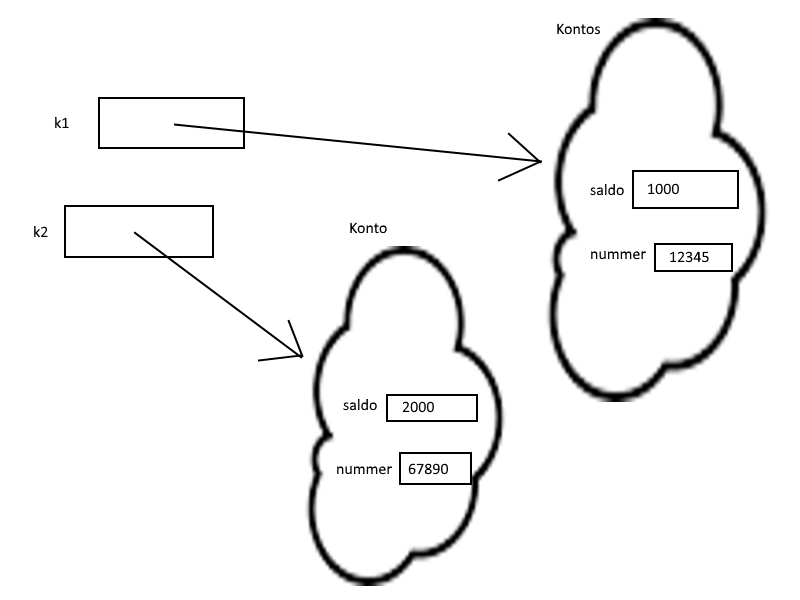
\includegraphics[scale=0.5]{../img/w04-solutions/uppgift-3a}
%
% \SubtaskSolved
% Tilldelningen på rad 8 \code{k1.nummer = 12345L} ger felmeddelande eftersom variablen är oföränderlig.
%
%
% \QUESTEND
%
%
%
%
% %%<AUTOEXTRACTED by mergesolu>%%      %Uppgift 3
%
%
%
%
% \WHAT{Klass med attribut som parametrar.}
%
% \QUESTBEGIN
%
% \Task  \what~  Om man vill ge attributen initialvärden när objektet skapas med \code{new}, kan man placera attributen i en parameterlista till klassen. Koden som körs när objektet skapas och attributen tilldelas sina initialvärden, kallas \textbf{konstruktor} \Eng{constructor}.
%
% \begin{REPL}
% scala> class Konto(var saldo: Int, val nummer: Long)
% scala> val k = new Konto(0, 12345L)
% scala> println("Konto: " + k.nummer + " Saldo:" + k.saldo)
% scala> println(k)
% scala> k.toString
% \end{REPL}
%
% \Subtask Den två sista raderna ovan skriver ut den identifierare som JVM använder för att hålla reda på objektet i sina interna datastrukturer. Vad skrivs ut?
%
% \Subtask Skapa ännu en instans av klassen Konto  med samma saldo och nummer som \code{k} ovan och spara den i \code{val k2} och undersök dess objektidentifierare. Får objekten \code{k} och \code{k2} olika objektidentifierare?
%
% \Subtask Sätt in olika belopp på respektive konto.
%
% \Subtask Vad händer om du försöker ändra attributet \code{nummer}?
%
% \Subtask\Pen Ibland räcker det fint med en tupel, men ofta vill man ha en klass istället. Beskriv några fördelar med en Konto-klassen ovan jämfört med en tupel av typen \code{(Int, Long)}.
%
% \begin{REPLnonum}
% scala> var k3 = (0, 12345L)
% scala> k3 = (k3._1 + 100, k3._2)
% \end{REPLnonum}
%
% \SOLUTION
%
%
% \TaskSolved \what
%
%
% \SubtaskSolved   \code{String = Konto@cd576}, där \code{Konto@cd576} är ett unikt namn som identifierar instansen.
%
% \SubtaskSolved   Ja.
%
% \SubtaskSolved
% \begin{REPLnonum}
% scala> k.saldo = 42
% scala> k2.saldo = 67
% \end{REPLnonum}
%
% \SubtaskSolved   Eftersom variablen är oföränderlig ges ett felmeddelande.
%
% \SubtaskSolved   En fördel med klass är att man kan specificera att variablen ska kunna vara föränderlig. En till är att man kan inkludera metoder i klassen som man vill kunna använda på värdena.
%
%
% \QUESTEND
%
%
%
%
% %%<AUTOEXTRACTED by mergesolu>%%      %Uppgift 4
%
%
%
%
% \WHAT{Publikt eller privat attribut?}
%
% \QUESTBEGIN
%
% \Task  \what~  Man kan förhindra att ett attribut syns utanför klassen med hjälp av nyckelordet \code{private}.
%
% \begin{REPL}
% scala> class Konto1(val nummer: Long){ var saldo = 0 }
% scala> val k1 = new Konto1(12345678901L)
% scala> k1.nummer
% scala> k1.saldo += 1000
% scala> class Konto2(val nummer: Long){ private var saldo = 0 }
% scala> val k2 = new Konto2(12345678901L)
% scala> k2.nummer
% scala> k2.saldo += 1000
% \end{REPL}
%
% \Subtask Vad händer ovan?
%
% \Subtask Gör en ny version av klassen \code{Konto} enligt nedan:
%
% \begin{Code}
% class Konto(val nummer: Long){
%   private var saldo = 0
%   def in(belopp: Int): Unit = {saldo += belopp}
%   def ut(belopp: Int): Unit = {saldo -= belopp}
%   def show: Unit =
%     println("Konto Nr: " + nummer + " saldo: " + saldo)
% }
%
% object Main {
%   def main(args: Array[String]): Unit = {
%     val k = new Konto(1234L)
%     k.show
%     k.in(1000)
%     println("Uttag: " + k.ut(500))
%     println("Uttag: " + k.ut(1000))
%     k.show
%   }
% }
% \end{Code}
%
% \Subtask Spara koden i en fil, kompilera med \code{scalac} och kör. Testa även vad som händer om du försöker komma åt attributet \code{saldo} i main-metoden med t.ex. \code{println(k.saldo)} eller \code{k.saldo += 1000}.
%
% \Subtask Vi ska nu förhindra överuttag. Ändra i metoden \code{ut} så att den får signaturen \code{ut(belopp: Int): (Int, Int) = ???} och implementera \code{ut} så att den returnerar både beloppet man verkligen kan ta ut och kvarvarande saldo. Om man försöker ta ut mer än det finns på kontot så ska saldot bli 0 och man får bara ut det som finns kvar. Spara, kompilera, kör.
%
% \Subtask Förbättra metoderna \code{in} och \code{ut} så att man inte kan sätta in eller ta ut negativa belopp.
%
% \Subtask Vad är fördelen med att göra föränderliga attribut privata och bara påverka deras värden indirekt via metoder?
%
% \SOLUTION
%
%
% \TaskSolved \what
%
%
% \SubtaskSolved
% Det går bra att ändra på variablen saldo i instansen av Konto1 men inte av Konto2 där man får ett error på raden ''k2.saldo += 1000''
%
% \SubtaskSolved  -
%
% \SubtaskSolved
% ''println(k.saldo)'' och ''k.saldo += 1000'' ger båda error, pga privat attribut.
%
% \SubtaskSolved
% \begin{Code}
% def ut(belopp: Int): (Int, Int) = {
% 	if(saldo >= belopp) {
% 		saldo -= belopp
% 		(belopp, saldo)
% 	} else {
% 		val temp = saldo
% 		saldo = 0
% 		(temp, 0)
% 	}
% }
% \end{Code}
%
% \SubtaskSolved
% Lägg till en if-sats i båda funktionerna som omsluter den gamla koden.
% \begin{Code}
% def ut(belopp: Int): (Int, Int) = {
%   if(belopp >= 0) {
%     if(saldo >= belopp) {
%       saldo -= belopp
%       (belopp, saldo)
%     } else {
%       val temp = saldo
%       saldo = 0
%       (temp, 0)
%     }
%   }
% }
%
% def in(belopp: Int): Unit = {
%   if(belopp >= 0) {
%     saldo += belopp
%   }
% }
% \end{Code}
%
% \SubtaskSolved
% Genom att göra attributet privat och gör egna metoder kan man se till att attriuten endast ändras på säkra sätt. Så inte fel uppstår.
%
%
% \QUESTEND
%
%
%
%
% %%<AUTOEXTRACTED by mergesolu>%%      %Uppgift 5
%
%
%
%
% \WHAT{Vilken typ har ett objekt?}
%
% \QUESTBEGIN
%
% \Task  \what~  Objektets typ bestäms av klassen. Vid tilldelning måste typerna passa ihop.
%
% \Subtask Vilka rader nedan ger felmeddelande? Hur lyder felmeddelandet?
% \begin{REPL}
% scala> class Punkt(val x: Double, val y: Double)
% scala> val pt: Punkt = new Punkt(10.0, 10.0)
% scala> val i: Int = pt.x
% scala> val (x: Double, y: Double) = (pt.x, pt.y)
% scala> val p: Double = new Punkt(5.0, 5.0)
% scala> val p = new Punkt(5.0, 5.0): Double
% scala> val p = new Punkt(5.0, 5.0): Punkt
% scala> pt: Punkt
% \end{REPL}
%
%
% \Subtask Man kan undersöka om ett objekt är av en viss typ med metoden \\ \code{isInstanceOf[Typnamn]}. Vad ger nedan anrop av metoden \code{isInstanceOf} för värde?
% \begin{REPL}
% scala> class Punkt(val x: Double, val y: Double)
% scala> val pt: Punkt = new Punkt(1.0, 2.0)
% scala> pt.isInstanceOf[Punkt]
% scala> pt.isInstanceOf[Double]
% scala> pt.x.isInstanceOf[Punkt]
% scala> pt.x.isInstanceOf[Double]
% scala> pt.x.isInstanceOf[Int]
% \end{REPL}
%
% \SOLUTION
%
%
% \TaskSolved \what
%
%
% \SubtaskSolved
% ''val i: Int = pt.x'' error: type mismatch;
% Eftersom typen Int ej är kompatibel med ett värde av typen Double.
%
% ''val p: Double = new Punkt(5.0, 5.0)'' error: type mismatch;
% Eftersom typen Double ej är kompatibel med ett värde av typen Punkt.
%
% ''val p = new Punkt(5.0, 5.0): Double'' error: type mismatch;
% Eftersom typen Double ej är kompatibel med ett värde av typen Punkt.
%
% \SubtaskSolved
% Rad 3 till 7 i respektive ordning: true, false, false, true och false.
%
%
% \QUESTEND
%
%
%
%
% %%<AUTOEXTRACTED by mergesolu>%%      %Uppgift 6
%
%
%
%
% \WHAT{Topptypen \code{Any}.}
%
% \QUESTBEGIN
%
% \Task  \what~ Alla klasser är också av typen \code{Any}. Alla klasser får därmed med sig några gemensamma metoder som finns i den fördefinierade klassen \code{Any}, däribland metoderna  \code{isInstanceOf} och \code{toString}.  Vad blir resultatet av respektive rad nedan? Vilken rad ger ett felmeddelande?
%
%
% \begin{REPL}
% scala> class Punkt(val x: Double, val y: Double)
% scala> val pt: Punkt = new Punkt(1.0, 2.0)
% scala> pt.isInstanceOf[Punkt]
% scala> pt.isInstanceOf[Any]
% scala> pt.x.toString
% scala> println(pt.x)
% scala> val a: Any = pt
% scala> println(a.x)
% scala> a.toString
% scala> pt.y.toString
% scala> a.y.toString
% \end{REPL}
%
% \SOLUTION
%
%
% \TaskSolved \what
%
% \begin{enumerate}
% \item Definierar klassen Punkt.
% \item En variabel pt: Punkt skapas.
% \item true
% \item true
% \item String = 1.0
% \item skriver ut: 1.0
% \item En variabel med namnet a skapas med typen Any.
% \item error: value x is not a member of Any
% \item a ges nu typen String
% \item String = 2.0
% \item error: value y is not a member of Any
% \end{enumerate}
%
%
% \QUESTEND
%
%
%
%
% %%<AUTOEXTRACTED by mergesolu>%%      %Uppgift 7
%
%
%
%
% \WHAT{Byta ut metoden \code{toString}}.
%
% \QUESTBEGIN
%
% \Task  \what~ I klassen \code{Any} finns metoden \code{toString} som skapar en strängrepresentation av objektet. Du kan byta ut metoden \code{toString} i klassen \code{Any} mot din egen implementation. Man använder nyckelordet \code{override} när man vill byta ut en metodimplementation.
%
% \begin{REPL}
% scala> class Punkt(val x: Double, val y: Double) {
%          override def toString: String = "[x=" + x + ",y=" + y + "]"
%        }
% scala> val pt = new Punkt(1.0, 42.0)
% scala> pt.toString
% scala> println(pt)
% \end{REPL}
%
% \Subtask Vad händer egentligen på sista raden ovan?
%
% \Subtask Omdefiniera toString så att den ger en sträng på formen \code{Punkt(1.0, 42.0)}.
%
% \Subtask Vad händer om du utelämnar nyckelordet \code{override} vid omdefiniering?
%
% \SOLUTION
%
%
% \TaskSolved \what
%
%
% \SubtaskSolved
% ''println(pt)'' kallar på pt.toString, och eftersom metoden är överskriven kallas den nya version.
%
% \SubtaskSolved   \code{override def toString: String = ''Punkt('' + x + '', '' + y + '').''}
%
% \SubtaskSolved
% error: overriding method toString in class Object of type ()String;
%
%
% \QUESTEND
%
%
%
%
% %%<AUTOEXTRACTED by mergesolu>%%      %Uppgift 8
%
%
%
%
% \WHAT{Objektfabrik med \code{apply}-metod.}
%
% \QUESTBEGIN
%
% \Task  \what~  Man kan ordna så att man slipper skriva \code{new} med ett s.k. \emph{fabriksobjekt} \Eng{factory object}.
% \begin{Code}
% class Pt(val x: Double, y: Double) {
%   override def toString: String = "Pt(x=" + x + ",y=" + y + ")"
% }
% object Pt {
%   def apply(x: Double, y: Double): Pt = new Pt(x, y)
% }
% \end{Code}
%
% \Subtask Skriv satser som använder metoden \code{apply} i fabriksobjektet \code{object Pt} för att skapa flera olika punkter.
%
% \Subtask Ge applymetoden default-argument 0.0 för både x och y så att \code{Pt()} skapar en punkt i origo.
%
% \Subtask Skapa en klass \code{Rational} som representerar rationellt tal som en kvot mellan två heltal. Ge klassen två oföränderliga, publika klassparameterattribut med namnen \code{nom} för täljaren och \code{denom} för nämnaren.
%
% \Subtask Skapa ett fabriksobjekt med en \code{apply}-metod som tar två heltalsparametrar och skapar en instans av klassen \code{Rational}.
%
% \Subtask Skapa olika instanser av din klass \code{Rational} ovan med hjälp av fabriksobjektet.
%
%
% \SOLUTION
%
%
% \TaskSolved \what
%
%
% \SubtaskSolved
% \begin{REPL}
% scala> val pt = Pt(1.0, 2.0)
% pt: Pt = Pt(x=1.0,y=2.0)
%
% scala> Pt(4.0, 2.0)
% res0: Pt = Pt(x=4.0,y=2.0)
%
% scala> Pt(6.0, 3.0)
% res1: Pt = Pt(x=6.0,y=3.0)
%
% scala> Pt(666.0, 1337.0)
% res2: Pt = Pt(x=666.0,y=1337.0)
% \end{REPL}
%
% \SubtaskSolved  \code{def apply(): Pt = new Pt(0, 0)}
%
% \SubtaskSolved  \code{class Rational(val nom: Int, val denom: Int)}
%
% \SubtaskSolved
% \begin{REPLnonum}
% object Rational {
% def apply(nom: Int, denom: Int): Rational = new Rational(nom, denom)
% }
% \end{REPLnonum}
%
% \SubtaskSolved
% \begin{REPL}
% scala> Rational(2, 5)
% scala> Rational(2, 7)
% scala> Rational(7, 4)
% scala> Rational(666, 1337)
% \end{REPL}
%
%
% \QUESTEND
%
%
%
%
% %%<AUTOEXTRACTED by mergesolu>%%      %Uppgift 9
%
%
%
%
% \WHAT{Skapa en case-klass.}
%
% \QUESTBEGIN
%
% \Task  \what~  Med en case-klass får man \code{toString} och fabriksobjekt på köpet. Man behöver inte skriva \code{val} framför klassparametrar i case-klasser; klassparametrar blir publika, oföränderliga attribut automatiskt när man deklarerar en case-klass.
%
% \begin{REPL}
% scala> case class Pt(x: Double, y: Double)
% scala> val p = Pt(1.0, 42.0)
% scala> p.toString
% scala> println(p)
% scala> println(Pt(5,6))
% \end{REPL}
%
% \Subtask Implementera din klass \code{Rational} från föregående uppgift, men nu som en case-klass.
%
% \SOLUTION
%
%
% \TaskSolved \what
%
% \SubtaskSolved  \code{case class Rational(nom: Int, denom: Int)}
%
%
% \QUESTEND
%
%
%
%
% %%<AUTOEXTRACTED by mergesolu>%%      %Uppgift 10
%
%
%
%
% \WHAT{Metoder på datastrukturer.}
%
% \QUESTBEGIN
%
% \Task \label{task:point} \what~   En datastruktur blir mer användbar om det finns metoder som kan användas på datastrukturen. Metoder i Scala kan även ha (vissa) specialtecken som namn, t.ex. \code{+} enligt nedan.
% \begin{REPL}
% scala> case class Point(x: Double, y: Double) {
%          def distToOrigin: Double = math.hypot(x, y)
%          def add(p: Point): Point = Point(x + p.x, y + p.y)
%          def +(p: Point): Point = add(p)
%        }
% \end{REPL}
%
% \Subtask Använd metoden \code{distToOrigin} för att ta reda på vad punkten med koordinaterna (3, 4) har för avstånd till origo?
%
% \Subtask Skriv satser som skapar två punkter (3,4) och (5, 6) och låt variablerna p1 och p2 referera till respektive punkt. Låt variabeln p3 bli summan av p1 och p2 med hjälp av metoden \code{add}. Vad får uttrycken \code{p3.x} resp. \code{p3.y} för värden?
%
%
%
% \SOLUTION
%
%
% \TaskSolved \what
%
%
% \SubtaskSolved
% \begin{REPLnonum}
% scala> Point(3, 4).distToOrigin
% res0: Double = 5.0
% \end{REPLnonum}
%
% \SubtaskSolved
% p3.x = 8
% p3.y = 10
%
%
% \QUESTEND
%
%
%
%
% %%<AUTOEXTRACTED by mergesolu>%%      %Uppgift 11
%
%
%
%
% \WHAT{Operatornotation.}
%
% \QUESTBEGIN
%
% \Task  \what~  Vid punktnotation på formen: \\ \code{objekt.metod(argument)} \\ kan man skippa punkten och parenteserna och skriva:\\ \code{objekt metod argument}  \\
% Detta förenklade skrivsätt kallas \textbf{operatornotation}.
%
% \Subtask Använd klassen \code{Point} från uppgift \ref{task:point} och prova nedan satser. Vilka rader använder operatortnotation och vilka rader använder punktnotation? Vilka rader ger felmeddelande?
% \begin{REPL}
% scala> val p1 = Point(3,4)
% scala> val p2 = Point(3,4)
% scala> p1.add(p2)
% scala> p1 add p2
% scala> p1.+(p2)
% scala> p1 + p2
% scala> 42 + 1
% scala> 42.+(1)
% scala> 42.+ 1
% scala> 42 +(1)
% scala> 1.to(42)
% scala> 1 to 42
% scala> 1.to(42)
% \end{REPL}
%
% \Subtask Implementera metoderna \code{sub} och \code{-} i klassen \code{Point} och skriv uttryck som kombinerar add och sub, samt + och - i både punktnotation och operatornotation.
%
% \Subtask Operatornotation fungerar även med flera argument. Man använder då parenteser om listan med argumenten:
% \code{ objekt metod (arg1, arg2)}  \\
% Definiera en metod \\
% \code{def scale(a: Double, b: Double) = Point(x * a, y * b)} \\
% i klassen \code{Point} och skriv satser som använder metoden med punktnotation och operatornotation.
%
%
%
%
%
% \SOLUTION
%
%
% \TaskSolved \what
%
%
% \SubtaskSolved
% \\Operatornotation:	4, 6, 10, 12
% \\Punktnotation:		3, 5, 8, 9, 11, 13
% \\Felmeddelande:		9
%
% \SubtaskSolved
% \begin{Code}
% case class Point(x: Double, y: Double) {
%   def distToOrigin: Double = math.hypot(x, y)
%   def add(p: Point): Point = Point(x + p.x, y + p.y)
%   def +(p: Point): Point = add(p)
%   def sub(p: Point): Point = Point(x - p.x, y - p.y)
%   def -(p: Point): Point = sub(p)
% }
% \end{Code}
% \begin{REPL}
% scala> val p1: Point = Point(1, 9)
% scala> val p2: Point = Point(9, 6)
% scala> p1.sub(p2)
% scala> p1.-(p2)
% scala> p2 sub p1
% scala> p2 - p2
% scala> p1.add(p2.sub(p1))
% scala> p1 + (p2 - p1)
% \end{REPL}
%
% \SubtaskSolved
% \begin{Code}
% case class Point(x: Double, y: Double) {
%   def distToOrigin: Double = math.hypot(x, y)
%   def add(p: Point): Point = Point(x + p.x, y + p.y)
%   def +(p: Point): Point = add(p)
%   def sub(p: Point): Point = Point(x - p.x, y - p.y)
%   def -(p: Point): Point = sub(p)
%   def scale(a: Double, b: Double) = Point(x * a, y * b)
% }
% \end{Code}
% \begin{REPL}
% scala> val p: Point(13,  37)
% scala> p.scale(4, 2)
% scala> p scale (3, 7)
% \end{REPL}
%
%
% \QUESTEND
%
%
%
%
% %%<AUTOEXTRACTED by mergesolu>%%      %Uppgift 12
%
%
%
%
% \WHAT{Föränderlighet och oföränderlighet.}
%
% \QUESTBEGIN
%
% \Task  \what~  Oföränderliga och föränderliga objekt beter sig olika vid tilldelning.
%
% \Subtask\Pen Innan du kör nedan kod: Försök lista ut vad som kommer att skrivas ut. Rita minnessituationen efter varje tilldelning.
%
% \begin{Code}
% println("\n--- Example 1: mutable value assigmnent")
% var x1 = 42
% var y1 = x1
% x1 = x1 + 42
% println(x1)
% println(y1)
% \end{Code}
%
% \Subtask\Pen Innan du kör nedan kod: Försök lista ut vad som kommer att skrivas ut. Rita minnessituationen efter varje tilldelning.
%
% \begin{Code}
% println("\n--- Example 2: mutable object reference assignment")
% class MutableInt(private var i: Int) {
%   def +(a: Int): MutableInt = { i = i + a; this }
%   override def toString: String = i.toString
% }
% var x2 = new MutableInt(42)
% var y2 = x2
% x2 = x2 + 42
% println(x2)
% println(y2)
% \end{Code}
%
% \Subtask\Pen Innan du kör nedan kod: Försök lista ut vad som kommer att skrivas ut. Rita minnessituationen efter varje tilldelning.
%
% \begin{Code}
% println("\n--- Example 3: immutable object reference assignment")
% class ImmutableInt(val i: Int) {
%   def +(a: Int): ImmutableInt = new ImmutableInt(i + a)
%   override def toString: String = i.toString
% }
% var x3 = new ImmutableInt(42)
% var y3 = x3
% x3 = x3 + 42
% println(x3)
% println(y3)
% \end{Code}
%
% \Subtask\Pen Vad finns det för fördelar med oföränderliga datastrukturer?
%
%
% \SOLUTION
%
%
% \TaskSolved \what
%
%
% \SubtaskSolved   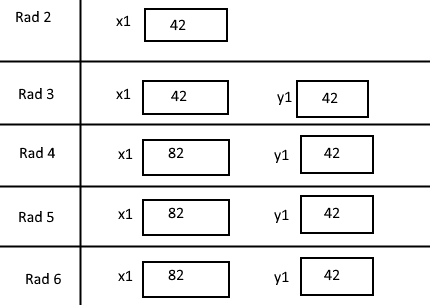
\includegraphics[scale=0.5]{../img/w04-solutions/uppgift-13a}
%
% \SubtaskSolved
% \begin{enumerate}
% \item 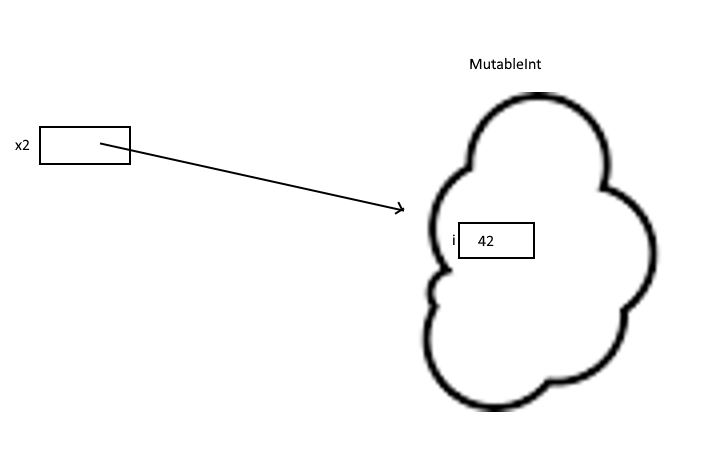
\includegraphics[scale=0.5]{../img/w04-solutions/uppgift-13b-1}
% \item 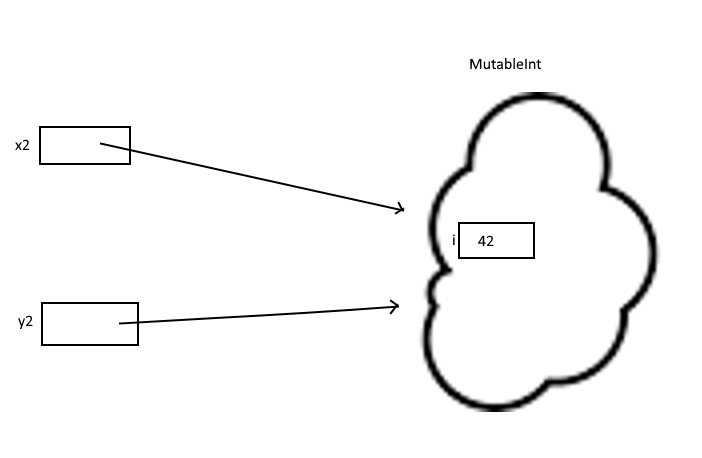
\includegraphics[scale=0.5]{../img/w04-solutions/uppgift-13b-2}
% \item 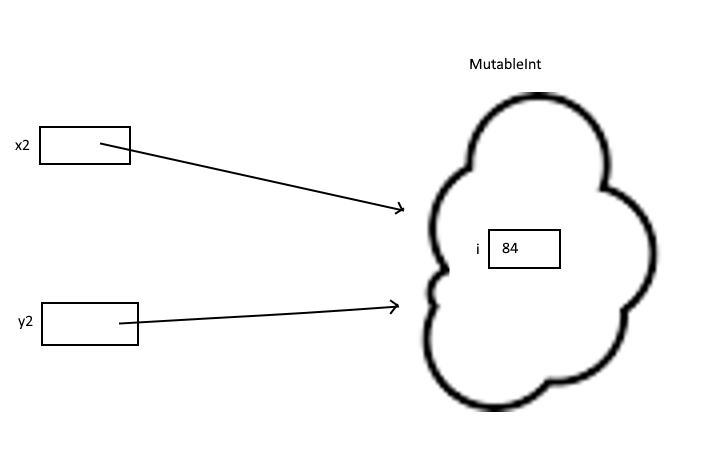
\includegraphics[scale=0.5]{../img/w04-solutions/uppgift-13b-3}
% \end{enumerate}
%
% \SubtaskSolved
% \begin{enumerate}
% \item 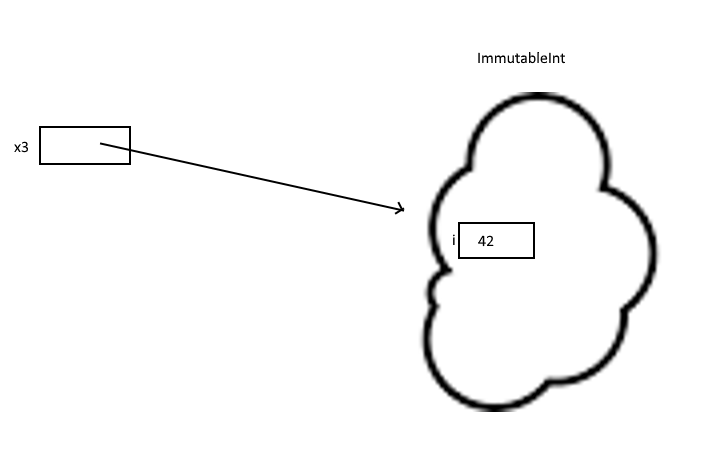
\includegraphics[scale=0.5]{../img/w04-solutions/uppgift-13c-1}
% \item 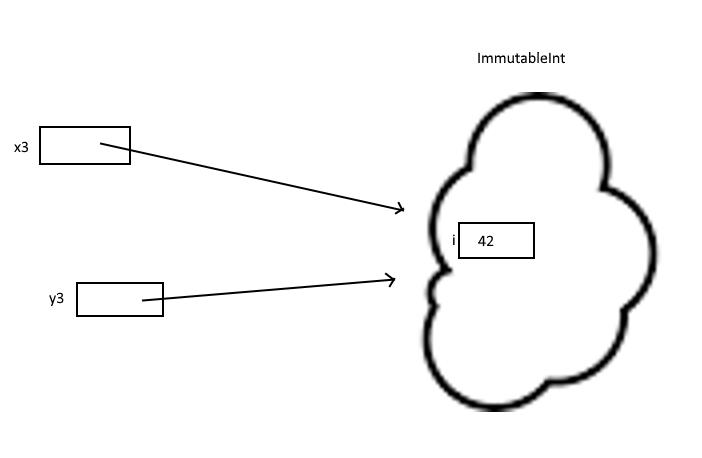
\includegraphics[scale=0.5]{../img/w04-solutions/uppgift-13c-2}
% \item 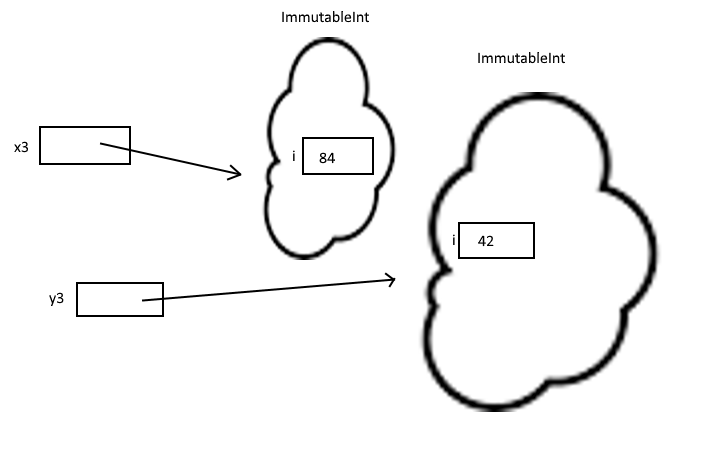
\includegraphics[scale=0.5]{../img/w04-solutions/uppgift-13c-3}
% \end{enumerate}
%
% \SubtaskSolved   En stor fördel är att vi till exempel kan skicka med en immutable som argument till en metod och vara säkra på att metoden inte ändrar på värdet.
%
%
% \QUESTEND
%
%
%
%
% %%<AUTOEXTRACTED by mergesolu>%%      %Uppgift 13
%
%
%
%
% \WHAT{Några användbara samlingar.}
%
% \QUESTBEGIN
%
% \Task  \what~  En \textbf{samling} \Eng{collection} är en datastruktur som samlar många objekt av samma typ. I \code{scala.collection} och \code{java.util} finns många olika samlingar med en uppsjö användbara metoder. De olika samlingarna i \code{scala.collection} är ordnade i en gemensam hierarki med många gemensamma metoder; därför har man nytta av det man lär sig om metoderna i en Scala-samling när man använder en annan samling. Vi har redan tidigare sett samlingen \code{Vector}:
%
% \begin{REPL}
% scala> val tärningskast = Vector.fill(10000)((math.random * 6 + 1).toInt)
% scala> tä   // tryck TAB
% scala> tärningskast.  // tryck TAB
% \end{REPL}
%
% \Subtask Ungefär hur många metoder finns det som man kan göra på objekt av typen \code{Vector}? Det är svårt att lära sig alla dessa på en gång, så vi väljer ut några få i kommande uppgifter.
%
% \Subtask Jämför överlappet mellan metoderna i \code{Vector} och \code{List} och uppskatta hur stor andel av metoderna som är gemensamma:
% \begin{REPL}
% scala> val myntkast =
%          List.fill(10000)(if (math.random < 0.5) "krona" else "klave")
% scala> my   // tryck TAB
% scala> myntkast.  // tryck TAB
% \end{REPL}
%
% \SOLUTION
%
%
% \TaskSolved \what
%
%
% \SubtaskSolved   Ungefär 150 metoder.
%
% \SubtaskSolved   Ungefär lika många.
%
%
% \QUESTEND
%
%
%
%
% %%<AUTOEXTRACTED by mergesolu>%%      %Uppgift 14
%
%
%
%
% \WHAT{Typparameter.}
%
% \QUESTBEGIN
%
% \Task  \what~  Vissa funktioner är generella för många typer och tar en så kallad \textbf{typparameter} inom hakparenteser. Ofta slipper man skriva typparametrar, då kompilatorn kan härleda typen utifrån argumenten. Om man anger typparametrar explicit så hjälper kompilatorn dig med att kolla att det verkligen är rätt typ i samlingen.
%
% \Subtask Vad händer nedan?
% \begin{REPL}
% scala> var xs = Vector.empty[Int]
% scala> xs = xs :+ "42"
% scala> xs = xs :+ 43 :+ 64 :+ 46
% scala> xs
% scala> xs :+= "42".toInt
% scala> var ys = Vector[Int]("ett", "två", "tre")
% scala> var ingenting = Vector.empty
% scala> ingenting = Vector(1,2,3)
% \end{REPL}
%
% \Subtask Samlingar är mer användbara om de är \emph{generiska}, vilket innebär att elementens typ avgörs av en typparameter och därför kan vara av vilken typ som helst. Man kan definiera egna funktioner som tar generiska samlingar som parametrar. Förklara vad som händer här:
% \begin{REPL}
% scala> val vego = Vector("gurka", "tomat", "apelsin", "banan")
% scala> val prim = Vector(2, 3, 5, 7, 11, 13)
% scala> def först[T](xs: Vector[T]): T = xs.head
% scala> def sist[T](xs: Vector[T]) = xs.last
% scala> def förstOchSist[T](xs: Vector[T]): (T, T) = (xs.head, xs.last)
% scala> först(vego)
% scala> sist(prim)
% scala> förstOchSist(vego)
% scala> förstOchSist(prim)
% scala> def wrap[T](pair: (T, T))(xs: Vector[T]) = pair._1 +: xs :+ pair._2
% scala> wrap("Odla", "och ät!")(vego)
% scala> wrap("Odla", "och ät!")(vego).mkString(" ")
% \end{REPL}
%
%
%
%
%
% \SOLUTION
%
%
% \TaskSolved \what
%
%
% \SubtaskSolved
% \\1. Instansierar en tom vektor med element av typen int och tilldelar värdet till en variabel xs.
% \\2. Error eftersom \code{xs :+ ''42''} ger en Vector[Any] när Vector[Int] krävs.
% \\3. xs tilldelas ett nytt värde av Vector(43, 64, 46)
% \\4. xs skrivs ut.
% \\5. Lägger till talet 42 i xs.
% \\6. Error: type mismatch
% \\7. Skapar en tom Vector i variablen ingenting
% \\8. error: type mismatch; found: Int(3), required: Nothing
%
% \SubtaskSolved
% Tre metoder skapas: den första för att få första elementet i en lista, och eftersom den definieras med specialtypen T går den att använda med alla vektorer oavsett typen av variabeln i vektorn. Den andra får fram sista elementet och den sista hämtar båda två.
%
% En till function definieras längre ner med  namnet ''wrap'', som tar en lista och lägger till ett element längst fram och ett längst bak.
%
%
% \QUESTEND
%
%
%
%
% %%<AUTOEXTRACTED by mergesolu>%%      %Uppgift 15
%
%
%
%
% \WHAT{Några viktiga samlingsmetoder.}
%
% \QUESTBEGIN
%
% \Task  \what~  Deklarera följande vektorer i REPL.
% \begin{REPL}
% scala> val xs = (1 to 10).toVector
% scala> val a = Vector("abra", "ka", "dabra")
% scala> val b = Vector( "sim", "sala", "bim", "sala", "bim")
% scala> val stor = Vector.fill(100000)(math.random)
% \end{REPL}
% Undersök i REPL vad som händer nedan. Alla dessa metoder fungerar på alla samlingar som är indexerbara sekvenser. Givet deklarationerna ovan: vad har uttrycken nedan för värde och typ? Förklara vad som händer hälp av denna  översikt: \href{http://docs.scala-lang.org/overviews/collections/seqs}{docs.scala-lang.org/overviews/collections/seqs}
%
% \Subtask \code{a(1) + xs(1)}
%
% \Subtask \code{a apply 0}
%
% \Subtask \code{a.isDefinedAt(3)}
%
% \Subtask \code{a.isDefinedAt(100)}
%
% \Subtask \code{stor.length}
%
% \Subtask \code{stor.size}
%
% \Subtask \code{stor.min}
%
% \Subtask \code{stor.max}
%
% \Subtask \code{a indexOf "ka"}
%
% \Subtask \code{b.lastIndexOf("sala")}
%
% \Subtask \code{"först" +: b   //minnesregel: colon on the collection side}
%
% \Subtask \code{a :+ "sist"    //minnesregel: colon on the collection side}
%
% \Subtask \code{xs.updated(2,42)}
%
% \Subtask \code{a.padTo(10, "!")}
%
% \Subtask \code{b.sorted}
%
% \Subtask \code{b.reverse}
%
% \Subtask \code{a.startsWith(Vector("abra", "ka"))}
%
% \Subtask \code{"hejsan".endsWith("san")}
%
% \Subtask \code{b.distinct}
%
%
%
% \SOLUTION
%
%
% \TaskSolved \what
%
%
% \SubtaskSolved   String = ''ka2''
%
% \SubtaskSolved   String = ''abra''
%
% \SubtaskSolved   false
%
% \SubtaskSolved   false
%
% \SubtaskSolved   100000
%
% \SubtaskSolved   100000
%
% \SubtaskSolved   minsta talet i listan
%
% \SubtaskSolved   största talet i listan
%
% \SubtaskSolved   1
%
% \SubtaskSolved   3
%
% \SubtaskSolved   Vektor b fast med ''först'' som första element
%
% \SubtaskSolved   Vektor a fast med ''sist'' som sista element.
%
% \SubtaskSolved   plats 3 i vektorn xs får värdet 42
%
% \SubtaskSolved   En ny vektor fylld med ''!'' från och med plats 4 till 10. Men de andra värdena samma som i a.
%
% \SubtaskSolved   b sorterad i bokstavsordning
%
% \SubtaskSolved   b baklänges
%
% \SubtaskSolved   true
%
% \SubtaskSolved   true
%
% \SubtaskSolved   en vektor med alla unika element i b.
%
%
% \QUESTEND
%
%
%
%
% %%<AUTOEXTRACTED by mergesolu>%%      %Uppgift 16
%
%
%
%
% \WHAT{Några generella samlingsmetoder.}
%
% \QUESTBEGIN
%
% \Task  \what~  Det finns metoder som går att köra på \emph{alla} samlingar även om de inte är indexerbara. Givet deklarationerna i föregående uppgift: vad har uttrycken nedan för värde och typ? Förklara vad som händer med hjälp av dessa översikter: \\ \href{http://docs.scala-lang.org/overviews/collections/trait-traversable}{docs.scala-lang.org/overviews/collections/trait-traversable} \\ \href{http://docs.scala-lang.org/overviews/collections/trait-iterable}{docs.scala-lang.org/overviews/collections/trait-iterable}
%
% \Subtask \code{a ++ b}
%
% \Subtask \code{a ++ stor}
%
% \Subtask \code{val ys = xs.map(_ * 5)}
%
% \Subtask \code{b.toSet     // En mängd har inga dubletter}
%
% \Subtask \code{a.head + b.last}
%
% \Subtask \code{a.tail}
%
% \Subtask \code{a.head +: a.tail == a}
%
% \Subtask \code{Vector(a.head) ++ Vector(b.last)}
%
% \Subtask \code{a.take(1) ++ b.takeRight(1)}
%
% \Subtask \code{a.drop(2) ++ b.drop(1).dropRight(2)}
%
% \Subtask \code{a.drop(100)}
%
% \Subtask \code{val e = Vector.empty[String]; e.take(100)}
%
% \Subtask \code{Vector(e.isEmpty, e.nonEmpty)}
%
% \Subtask \code{a.contains("ka")}
%
% \Subtask \code{"ka" contains "a"}
%
% \Subtask \code{a.filter(s => s.contains("k")) }
%
% \Subtask \code{a.filter(_.contains("k")) }
%
% \Subtask \code{a.map(_.toUpperCase).filterNot(_.contains("K")) }
%
% \Subtask \code{xs.filter(x => x % 2 == 0)}
%
% \Subtask \code{xs.filter(_ % 2 == 0)}
%
%
% \SOLUTION
%
%
% \TaskSolved \what
%
%
% \SubtaskSolved
% Metoden ger tillbaka en ny Vector[String] som nu består av alla element i a plus alla element i b. I samma ordning med elementen i a först.
%
% \SubtaskSolved
% Samma som i uppgift a fast vektorn som returnas är av typen Vector[Any]. Det är eftersom Any är den närmsta typen som String och Double delar. Elementen från vektor a är fortfarande först och uppföljt av elementen i stor.
%
% \SubtaskSolved
% Variablen ys får värdet av en Vector[Int] som innehåller alla talen från xs fast multiplicerade med 5. Alltså ys = 5, 10, 15..., osv.
%
% \SubtaskSolved
% Functionen tar alla värden från en Vektor och sätter in i ett Set (mängd). Eftersom en mängd ej har dubletter så försvinner ett ''sala'' och ett ''bim'', Vector[String] som returneras blir därför (''sim'', ''sala'', ''bim'').
%
% \SubtaskSolved
% Metoden head ger första elementet i en samling, och last sista. Därför blir kombinationen av a.head och b.last en ny Vector[String] som består av a:s första element, och b:s första element.
%
% \SubtaskSolved
% Ger en Vector[String] som innehåller alla element efter det första. Alltså i detta fallet ''ka'' och ''dabra''.
%
% \SubtaskSolved
% True, eftersom head ger första elementet och tail ger resten, sedan sätter metoden +: ihop dem till en vektor med samma värden som a.
%
% \SubtaskSolved
% Eftersom ++ sätter ihop alla värden från två vektorer måste vi först omvandla från en sträng till vektor. Resultatet blir en ny vektor av samma typ som innan med a:s första element och b:S sista.
%
% \SubtaskSolved
% Samma resultat som i h, metoden take börjar från vänster och tar så många element som man skickar med som parameter och gör till en ny lista. Med 1 som parameter motsvarar det att göra Vector(a.head). Metoden takeRight gör samma sak fast från höger.
%
% \SubtaskSolved
% Metoden drop är motsvarigheten till take fast exkluderar de specifierade elementen istället för att inkludera dem i vektorn.
%
% \SubtaskSolved
% Eftersom a endast innehåller 3 element returnerar drop(100) en tom vektor.
%
% \SubtaskSolved
% Returnerar en tom vektor med element typen String
%
% \SubtaskSolved
% returnerar Vector(true, false)
%
% \SubtaskSolved
% True, metoden contains kollar om en samling innehåller ett specifikt element.
%
% \SubtaskSolved
% True. Eftersom en sträng även kan ses som Vector[Char].
%
% \SubtaskSolved
% Filtrerar vektorn a till att endast innehålla strängar som innehåller k.
%
% \SubtaskSolved
% Exakt samma som i p
%
% \SubtaskSolved
% map(\_.toUpperCase) omvandlar alla strängar i a till stora bokstäver
% filterNot(\_.contains(''K'')) tar resultatet vi precis fick och tar bort alla strängar som innehåller stora K.
%
% \SubtaskSolved
% filtrerar så att endast jämna tal finns kvar.
%
% \SubtaskSolved
% Exakt samma som i s
%
%
%
%
% \QUESTEND
%
%
%
%
% %%<AUTOEXTRACTED by mergesolu>%%      %Uppgift 17
%
%
%
%
% \WHAT{NEEDS A TOPIC DESCRIPTION}
%
% \QUESTBEGIN
%
% \Task  \what~ De olika samlingarna i \code{scala.collection} används flitigt i andra paket, exempelvis \code{scala.util} och \code{scala.io}.
%
% \Subtask Vad händer här? (Metoden \code{shuffle} skapar en ny samling med elementen i slumpvis ordning.)
% \begin{REPL}
% val xs = Vector(1,2,3)
% def blandat = scala.util.Random.shuffle(xs)
% def test = if (xs == blandat) "lika" else "olika"
% (for(i <- 1 to 100) yield test).count(_ == "lika")
% \end{REPL}
%
%
% \Subtask Skapa en textfil med namnet \code{fil.txt} som innehåller lite text och läs in den med: \\\code{scala.io.Source.fromFile("fil.txt", "UTF-8").getLines.toVector}
% \begin{REPL}
% > cat > fil.txt
% hejsan
% svejsan
% > scala
% scala> val xs = scala.io.Source.fromFile("fil.txt", "UTF-8").getLines.toVector
% scala> xs.foreach(println)
% \end{REPL}
%
%
% \Subtask Vad händer här? (Metoden \code{trim} på värden av typen \code{String} ger en ny sträng med blanktecken i början och slutet borttagna.)
% \begin{REPL}
% scala> val pgk =
%   scala.io.Source.fromURL("http://cs.lth.se/pgk/","UTF-8").getLines.toVector
% scala> pgk.foreach(println)
% scala> pgk.map(_.trim).
%          filterNot(_.startsWith("<")).
%          filterNot(_.isEmpty).
%          foreach(println)
% \end{REPL}
%
%
%
% \SOLUTION
%
%
% \TaskSolved \what
%
%
% \SubtaskSolved
% Vi instansierar en vektor xs med talen 1, 2 och 3.
% sedan definierar vi en metod blandat som ger oss en randomiserad version av xs.
% sedan definierar vi en till metod som testar om xs är lika med resultatet från blandat. Om det är så returnerar den strängen ''lika'' annars ''olika''.
% Sist kör vi en for-loop där vi 100 gånger kör testet, samtidigt räknas hur många gånger ''lika'' returneras.
%
% Vårt resultat är en siffra på hur många gånger xs var samma som en blandad version av sig själv, eftersom det finns 6 permutationer med 3 variabler så borde det vara ungefär 1/6 chans.
%
% \SubtaskSolved  -
%
% \SubtaskSolved
% \\ \code{map(\_.trim)} tar bort alla onödiga mellanrum i början och slutet på varje rad
% \\ \code{filterNot(\_.startsWith(''<''))} filtrerar bort alla rader som börjar med strängen ''<''
% \\ \code{filterNot(\_.isEmpty)} filtrerar bort alla tomma rader.
% \\ \code{foreach(println)} skriver ut alla rader.
%
%
% \QUESTEND
%
%
%
%
% %%<AUTOEXTRACTED by mergesolu>%%      %Uppgift 18
%
%
%
%
% \WHAT{Jämföra List och Vector.}
%
% \QUESTBEGIN
%
% \Task  \what~  En indexerbar sekvens av värden kallas vektor eller lista. I Scala finns flera klasser som kan kan indexeras, däribland klasserna \code{Vector} och \code{List}.
%
% \Subtask \emph{Likheter mellan \code{Vector} och \code{List}.} Kör nedan rader i REPL. Prova indexera i båda och studera hur stor andel av metoderna som är gemensamma.
% \begin{REPL}
% scala> val sv = Vector("en", "två", "tre", "fyra")
% scala> val en = List("one", "two", "three", "four")
% scala> sv(0) + sv(3)
% scala> en(0) + en(3)
% scala> sv. //tryck TAB
% scala> en. //tryck TAB
% \end{REPL}
%
% \Subtask \emph{Skillnader mellan \code{Vector} och \code{List}.} Klassen \code{Vector} i Scala har ''under huven'' en avancerad datastruktur i form av ett s.k. självbalanserande träd, vilket gör att \code{Vector} är snabbare än \code{List} på nästan allt, \emph{utom} att bearbeta elementen i \emph{början} av sekvensen; vill man lägga till och ta bort i början av en \code{List} så kan det ibland gå ungefär dubbelt så fort jämfört med \code{Vector}, medan alla andra operationer är lika snabba eller snabbare med \code{Vector}. Det finns ett fåtal speciella metoder, som bara finns i \code{List}, för att skapa en lista och lägga till i början av en lista. Vad händer nedan?
%
% \begin{REPL}
% scala> var xs = "one" :: "two" :: "three" :: "four" :: Nil
% scala> xs = "zero" :: xs
% scala> val ys = xs.reverse ::: xs
% \end{REPL}
%
%
% \SOLUTION
%
%
% \TaskSolved \what
%
%
% \SubtaskSolved
% I princip alla metoder delas, en lista har några fler t. ex. ''::'', '':::'', ''mapConserve'' osv.
%
% \SubtaskSolved
% Först skapas en lista med 4 sträng värden och instansierar variablen xs med det värdet.
% sedan skapar vi en ny lista, som består av ''zero'' + den gamla listan och ger värdet till xs.
% Sist instansierar vi en ny variabel ys, som får värdet av xs omvänd plus xs.
%
%
% \QUESTEND
%
%
%
%
% %%<AUTOEXTRACTED by mergesolu>%%      %Uppgift 19
%
%
%
%
% \WHAT{Mängd.}
%
% \QUESTBEGIN
%
% \Task  \what~  En mängd är en samling som garanterar att det inte finns några dubbletter. Det går dessutom väldigt snabbt, även i stora mängder, att kolla om ett element finns eller inte i mängden. Elementen i samlingen \code{Set} hamnar ibland, av effektivitetsskäl, i en förvånande ordning.
% \begin{REPL}
% scala> val s = Set("Malmö", "Stockholm", "Göteborg", "Köpenhamn", "Oslo")
% s: scala.collection.immutable.Set[String] =
%      Set(Oslo, Malmö, Köpenhamn, Stockholm, Göteborg)
%
% scala> val t = Set("Sverige", "Sverige", "Sverige", "Danmark", "Norge")
% t: scala.collection.immutable.Set[String] = Set(Sverige, Danmark, Norge)
% \end{REPL}
% Givet ovan deklarationer: vad blir värde och typ av nedan uttryck?
%
% \Subtask \code{s + "Malmö" == s}
%
% \Subtask \code{s ++ t}
%
% \Subtask \code{Set("Malmö", "Oslo").subsetOf(s)}
%
% \Subtask \code{s subsetOf Set("Malmö", "Oslo")}
%
% \Subtask \code{s contains "Lund"}
%
% \Subtask \code{s apply "Lund"}
%
% \Subtask \code{s("Malmö")}
%
% \Subtask \code{s - "Stockholm"}
%
% \Subtask \code{t - ("Norge", "Danmark", "Tyskland")}
%
% \Subtask \code{s -- t}
%
% \Subtask \code{s -- Set("Malmö", "Oslo")}
%
% \Subtask \code{Set(1,2,3) intersect Set(2,3,4)}
%
% \Subtask \code{Set(1,2,3) & Set(2,3,4)}
%
% \Subtask \code{Set(1,2,3) union Set(2,3,4)}
%
% \Subtask \code{Set(1,2,3) | Set(2,3,4)}
%
%
% \SOLUTION
%
%
% \TaskSolved \what
%
%
% \SubtaskSolved
% true, Boolean
%
% \SubtaskSolved
% En samling av alla värden i s och t, Set[String]
%
% \SubtaskSolved
% true, Boolean
%
% \SubtaskSolved
% false, Boolean
%
% \SubtaskSolved
% false, Boolean
%
% \SubtaskSolved
% false, Boolean
%
% \SubtaskSolved
% true, Boolean
%
% \SubtaskSolved
% Samlingen s utan elementet ''Stockholm'', Set[String]
%
% \SubtaskSolved
% Samlingen t utan elementen ''Norge'' och ''Danmark'', Set[String]
%
% \SubtaskSolved
% returnerar s, Set[String]
%
% \SubtaskSolved
% Samlingen s utan ''Malmö'' och ''Oslo'', Set[String]
%
% \SubtaskSolved
% Set(2, 3), Set[Int]
%
% \SubtaskSolved
% se deluppgift l
%
% \SubtaskSolved
% Set(1, 2, 3 ,4), Set[Int]
%
% \SubtaskSolved
% se deluppgift n
%
%
% \QUESTEND
%
%
%
%
% %%<AUTOEXTRACTED by mergesolu>%%      %Uppgift 20
%
%
%
%
% \WHAT{Slå upp värden från nycklar med \code{Map}.}
%
% \QUESTBEGIN
%
% \Task  \what~  Samlingen \code{Map} är mycket användbar. Med den kan man snabbt leta upp ett värde om man har en nyckel. Samlingen \code{Map} är en generalisering av en vektor, där man kan ''indexera'', inte bara med ett heltal, utan med vilken typ av värde som helst, t.ex. en sträng. Datastrukturen \code{Map} är en s.k. \emph{associativ array}\footnote{\href{https://en.wikipedia.org/wiki/Associative_array}{https://en.wikipedia.org/wiki/Associative\_array}}, implementerad som en s.k. \emph{hashtabell}\footnote{\href{https://en.wikipedia.org/wiki/Hash_table}{https://en.wikipedia.org/wiki/Hash\_table}}.
% \begin{REPL}
% scala> var huvudstad =
%   Map("Sverige" -> "Stockholm", "Norge" -> "Oslo", "Skåne" -> "Malmö")
% \end{REPL}
% Givet ovan variabel \code{huvudstad}, förklara vad som händer nedan?
%
% \Subtask \code{huvudstad apply "Skåne"}
%
% \Subtask \code{huvudstad("Sverige")}
%
% \Subtask \code{huvudstad.contains("Skåne")}
%
% \Subtask \code{huvudstad.contains("Malmö")}
%
% \Subtask \code{huvudstad += "Danmark" -> "Köpenhamn"}
%
% \Subtask \code{huvudstad.foreach(println)}
%
% \Subtask \code{huvudstad getOrElse ("Norge", "???") }
%
% \Subtask \code{huvudstad getOrElse ("Finland", "???") }
%
% \Subtask \code{huvudstad.keys.toVector.sorted}
%
% \Subtask \code{huvudstad.values.toVector.sorted}
%
% \Subtask \code{huvudstad - "Skåne"}
%
% \Subtask \code{huvudstad - "Jylland"}
%
% \Subtask \code{huvudstad = huvudstad.updated("Skåne","Lund") }
%
%
%
% \SOLUTION
%
%
% \TaskSolved \what
%
%
% \SubtaskSolved
% Returnerar strängen ''Malmö'' eftersom det värdet är indexerat på platsen ''Skåne''.
%
% \SubtaskSolved
% Returnerar strängen ''Stockholm'' eftersom det värdet är indexerat på platsen ''Sverige''.
%
% \SubtaskSolved
% true, eftersom huvudstad innehåller indexet ''Skåne''
%
% \SubtaskSolved
% false, eftersom huvudstad ej innehåller indexet ''Malmö''. Notera att det är index och inte värden vi
% kollar om det finns.
%
% \SubtaskSolved
% Lägger till indexet ''Danmark'' med värdet ''Köpenhamn'' i samlingen.
%
% \SubtaskSolved
% Skriver ut alla 2-tupler.
%
% \SubtaskSolved
% Returnerar ''Oslo'', Note: Om indexet ''Norge'' inte hade funnits hade ''???'' returnerats istället.
%
% \SubtaskSolved
% Returnerar ''???''
%
% \SubtaskSolved
% Returnerar en sorterar vektor med alla index.
%
% \SubtaskSolved
% Returnerar en sorterar vektor med alla värden.
%
% \SubtaskSolved
% Returnerar en ny mängd men med ''Skåne'' -> ''Malmö'' borttaget.
%
% \SubtaskSolved
% Returnerar huvudstad mängden eftersom det inte finns ett ''Jylland'' index att ta bort.
%
% \SubtaskSolved
% Uppdaterar indexet ''Skåne'' till att istället leda till värdet ''Lund''
%
%
% \QUESTEND
%
%
%
%
% %%<AUTOEXTRACTED by mergesolu>%%      %Uppgift 21
%
%
%
%
% \WHAT{Skapa Map från en samling.}
%
% \QUESTBEGIN
%
% \Task  \what~
%
% \Subtask Definiera denna vektor och undersök dess typ:
% \begin{Code}
% val pairs = Vector(
%   ("Björn", 46462229009L),
%   ("Maj", 46462221667L),
%   ("Gustav", 46462224906L))
% \end{Code}
%
% \Subtask Vad har variablen \code{telnr} nedan för typ: \\ \code{var telnr = pairs.toMap}
%
% \Subtask Använd \code{telnr} för att slå upp telefonnummer för Maj och Kim med hjälp av metoderna \code{apply} och \code{get}.
%
% \Subtask Använd metoden \code{getOrElse} vid upplagningar av \code{telnr} och ge \code{-1L} som telefonnummer i händelse av att ett nummer inte finns.
%
% \Subtask Lägg till \code{("Fröken Ur", 464690510L)} i \code{telnr}-mappen.
%
% \Subtask Skapa en \code{Vector[(String, String)]} enligt nedan, så att telefonnumret blir en sträng utan inledande landsnummer men med en nolla i riktnumret. Byt ut \code{???} mot lämpligt uttryck.
% \begin{REPL}
% scala> telnr.toVector.map(p => ???)
% res85: Vector[(String, String)] = Vector(("Björn", "0462229009"), ("Maj",
% "0462221667"), ("Gustav", "0462224906"), ("Fröken Ur", 04690510"))
%
% \end{REPL}
%
% \Subtask Använd vektorn i resultatet ovan för att skapa en ny \code{Map[String, String]} med nationella telefonnumer. Slå upp numret till Fröken Ur.
%
% \SOLUTION
%
%
% \TaskSolved \what
%
%
% \SubtaskSolved
% \begin{REPLnonum}
% pairs: scala.collection.immutable.Vector[(String, Long)] =
% 					Vector((Björn,444), (Maj,441), (Lucy,666))
% \end{REPLnonum}
%
% \SubtaskSolved
% Map[String, Long]
%
% \SubtaskSolved
% \begin{REPLnonum}
% scala> telnr(''Maj'')
% res0: Long = 441
%
% scala> telnr.get(''Maj'')
% res1: Option[Long] = Some(441)
%
% scala> telnr(''Kim'')
% java.util.NoSuchElementException: key not found: 'Kim
%   at scala.collection.MapLike$class.default(MapLike.scala:228)
%   at scala.collection.AbstractMap.default(Map.scala:59)
%   at scala.collection.MapLike$class.apply(MapLike.scala:141)
%   at scala.collection.AbstractMap.apply(Map.scala:59)
%   ... 32 elided
%
% scala> telnr.get(''Kim'')
% res2: Option[Long] = None
% \end{REPLnonum}
%
% \SubtaskSolved
% \begin{REPLnonum}
% scala> telnr.getOrElse(''Maj'', -1L)
% res0: Long = 441
%
% scala> telnr.getOrElse(''Kim'', -1L)
% res1: Long = -1
% \end{REPLnonum}
%
% \SubtaskSolved
% telnr += ''Fröken Ur'' -> 464690510L
%
% \SubtaskSolved
% telnr.toVector.map(p => p.\_1 -> (''0'' + p.\_2.toString.substring(2)))
%
% \SubtaskSolved
% Använd metoden toMap och apply.
%
%
%
%
% \QUESTEND
%
%
%
%
% %%<AUTOEXTRACTED by mergesolu>%%      %Uppgift 22
%
%
%
%
% \WHAT{Samlingsmetoden \code{maxBy}.}
%
% \QUESTBEGIN
%
% \Task  \what~  Med samlingsmetoden \code{maxBy} kan man själv definiera vad som ska maximeras. (Denna metod kommer du att behöva i veckans laboration.)
%
% \Subtask Förklara vad som händer nedan.
% \begin{REPL}
% scala> val xs = Vector((2,3), (1,5), (-1, 1), (7, 2))
% scala> xs.maxBy(x => x._1)
% scala> xs.maxBy(x => x._2)
% \end{REPL}
%
% \Subtask Om man bara använder en parameter i en anonym funktion, till exempel parametern \code{x} i lambdauttrycket \code{x => x + 1} \emph{en enda} gång, och kompilatorn kan gissa alla typer, kan man använda understreck som ''platshållare'' för att förkorta lambdauttrycket så här: \code{ _ + 1}
%
% Skriv uttrycken på raderna 2 och 3 i föregående deluppgift på ett kortare sätt med hjälp platshållarsyntax \Eng{place holder syntax}.
%
% \Subtask På motsvarande sätt kan man använda \code{minBy} för att välja vilken funktion som definierar minimum. Prova \code{minBy} på motsvarande sätt som i föregående deluppgifter.
%
% \SOLUTION
%
%
% \TaskSolved \what
%
%
% \SubtaskSolved   Metoden maxBy hämtar det element som är ''störst'', på rad två gör \code{x => x._1} att första värdet i tuplerna används för att bestämma vilken som är störst. Likt gör \code{x => x._2} på rad tre att istället det andra värdet används.
%
% \SubtaskSolved
% \begin{REPLnonum}
% scala> xs.maxBy(_._1)
% scala> xs.maxBy(_._2)
% \end{REPLnonum}
%
% \SubtaskSolved
% \begin{REPLnonum}
% scala> xs.minBy(_._1)
% scala> xs.minBy(_._2)
% \end{REPLnonum}
%
%
%
% \QUESTEND
%
%
%
%
%
%
%
%
% \WHAT{NEEDS A TOPIC DESCRIPTION}
%
% \QUESTBEGIN
%
% \Task  \what~ Skriv nedan program med en editor och kompilera från terminalen. Lägg till kod i huvudprogrammet som testar klassen \code{Account} och kompilera och kör. Utvidga sedan klassen \code{Account} med fler attribut och funktioner som du väljer själv.
%
% \begin{Code}
% class Account(val number: Long, val maxCredit: Int){
%   private var balance = 0
%
%   def deposit(amount: Int): Int = {
%     if (amount > 0) {balance += amount}
%     balance
%   }
%
%   def withdraw(amount: Int): (Int, Int) = if (amount > 0) {
%     val allowedWithdrawal =
%       if (amount < balance + maxCredit) amount
%       else balance + maxCredit
%     balance = balance - allowedWithdrawal
%     (allowedWithdrawal, balance)
%   } else (0, balance)
%
%   def show: Unit =
%     println("Account Nbr: " + number + " balance: " + balance)
% }
%
% object Main {
%   def main(args: Array[String]): Unit = {
%     ???
%   }
% }
% \end{Code}
%
%
%
% \SOLUTION
%
%
% \QUESTEND
%
%
%
%
%
%
% \WHAT{NEEDS A TOPIC DESCRIPTION}
%
% \QUESTBEGIN
%
% \Task \label{task:keno-set} \what~  Läs om reglerna för spelet Keno här: \\ \url{https://sv.wikipedia.org/wiki/Keno} och gör deluppgifterna nedan.
%
% \Subtask Skapa en klass \code{Keno} som kan användas för att genomföra en Kenodragning. Låt klassen ha ett privat attribut \code{balls} som är en föränderlig mängd med heltal och som från början är tom. Implementera lämpliga metoder i klassen för att användaren av klassen ska kunna dra nya slumpmässiga bollar som inte redan är dragna.
%
% \Subtask Skapa en \code{case class KenoBet(bet: Set[Int])} för att hålla reda vilka 11 bollar en viss person satsar på. Definiera en metod \\ \code{def numberOfHits(keno: Keno): Int = ???}\\ i case-klassen \code{KenoBet} som givet en kenodragning räknar ut hur många bollar som satsats rätt.
%
% \Subtask Skriv ett huvudprogram som simulerar en enkel Kenodragning. Låt två personer satsa på 11 slumpmässiga bollar, genomför en dragning av 20 bollar ur 70 möjliga och kontrollera sedan hur många bollar som personerna har prickat rätt.
%
%
%
%
%
% \SOLUTION
%
%
% \QUESTEND
%
%
%
%
%
%
% \WHAT{Dokumentationen för \code{Any}.}
%
% \QUESTBEGIN
%
% \Task  \what~  Undersök vilka metoder som finns i klassen Any här: \href{http://www.scala-lang.org/api/current/scala/Any.html}{http://www.scala-lang.org/api/current/scala/Any.html}. Prova några av metoderna i REPL.
%
% \SOLUTION
%
%
% \QUESTEND
%
%
%
%
%
%
% \WHAT{Dokumentationen för samlingar.}
%
% \QUESTBEGIN
%
% \Task  \what~  Leta upp metoden \code{tabulate} i dokumentationen för objektet \code{Vector} nästan längst ner i listan här: \\ \href{http://www.scala-lang.org/api/current/scala/collection/immutable/Vector.html}{http://www.scala-lang.org/api/current/scala/collection/immutable/Vector.html} \\Leta upp den variant av \code{tabulate} som har signaturen:\\ \code{def tabulate[A](n: Int)(f: (Int) => A): Vector[A] }\\ Klicka på den gråfyllda trekanten till vänster om signaturen som fäller ut beskrivningen
%
% \Subtask Förklara vad som händer här:
% \begin{REPLnonum}
% scala> Vector.tabulate(10)(i => i % 3)
% \end{REPLnonum}
%
% \Subtask Klicka på det blåa stora o-et överst på sidan, för att växla till klass-vyn och studera listan med alla metoder  i klassen \code{Vector}.
%
%
% \SOLUTION
%
%
% \QUESTEND
%
%
%
%
%
%
% \WHAT{Fler metoder på indexerbara sekvenser.}
%
% \QUESTBEGIN
%
% \Task  \what~  Deklarera följande vektorer i REPL.
% \begin{REPL}
% scala> val xs = (1 to 10).toVector
% scala> val a = Vector("abra", "ka", "dabra")
% scala> val b = Vector( "sim", "sala", "bim", "sala", "bim")
% \end{REPL}
% Undersök i REPL vad som händer nedan. Alla dessa metoder fungerar på alla samlingar som är indexerbara sekvenser. Vad har uttrycken för värde och typ? Förklara vad metoden gör. Studera även denna  översikt: \href{http://docs.scala-lang.org/overviews/collections/seqs}{docs.scala-lang.org/overviews/collections/seqs}
%
% \Subtask \code{b.indexWhere(s => s.startsWith("b"))}  % advanced
%
% \Subtask \code{a.indices}  % advanced
%
% \Subtask \code{xs.patch(1, Vector(42,43,44), 7)} % advanced
%
% \Subtask \code{xs.segmentLength(_ < 8, 2)} % advanced
%
% \Subtask \code{b.sortBy(_.reverse)}  % advanced
%
% \Subtask \code{b.sortWith((s1, s2) => s1.size < s2.size)} % advanced
%
% \Subtask \code{a.reverseMap(_.size)}	% advanced
%
% \Subtask \code{a intersect Vector("ka", "boom", "pow")} % advanced
%
% \Subtask \code{a diff Vector("ka")} % advanced
%
% \Subtask \code{a union Vector("ka", "boom", "pow")} % advanced
%
%
%
% \SOLUTION
%
%
% \QUESTEND
%
%
%
%
% \WHAT{NEEDS A TOPIC DESCRIPTION}
%
% \QUESTBEGIN
%
% \Task  \what~ För samlingen \code{List} finns en alternativ metod till \code{+:} som heter \code{::} och kallas ''cons'' och som i kombination med objektet \code{Nil} kan användas för att med alternativ syntax bygga listor. Läs om detta här: \\ \href{http://alvinalexander.com/scala/how-create-scala-list-range-fill-tabulate-constructors}{alvinalexander.com/scala/how-create-scala-list-range-fill-tabulate-constructors} \\ och hitta på några egna övningar för att undersöka hur cons och Nil fungerar. Metoder som slutar med kolon är högerassociativa. Läs mer om detta här: \href{http://www.artima.com/pins1ed/basic-types-and-operations.html#5.8}{http://www.artima.com/pins1ed/basic-types-and-operations.html\#5.8}\SOLUTION
%
%
% \QUESTEND


%!TEX encoding = UTF-8 Unicode
%!TEX root = ../exercises.tex

\ifPreSolution

\Exercise{\ExeWeekEIGHT}\label{exe:W08}

\begin{Goals}
\item Kunna skapa och använda matriser med nästlade strukturer av \code{Vector}.
\item Kunna iterera över elementen i en matris med nästlade \code{for}-satser och \code{for}-\code{yield}-uttryck, samt nästlad applicering av \code{map} respektive \code{foreach}.
\item Kunna skapa och använda funktioner som tar matriser som parametrar.
\item Kunna skapa en enkel generisk klass och enkla generiska funktioner med hjälp av en typparameter.
\item Kunna beskriva skillnader och likheter mellan Scala och Java vad gäller indexering och iterering i matriser implementerade med nästlade arrayer.
%\item Kunna skapa och använda matriser med hjälp inbyggda arrayer i Java.
%\item Kunna använda nästlade \code{for}-satser i Java för att iterera över elementen i en matris.
\end{Goals}

\begin{Preparations}
\item \StudyTheory{08}
\end{Preparations}

\BasicTasks

\else

\ExerciseSolution{\ExeWeekEIGHT}

\BasicTasks

\fi



\WHAT{Para ihop begrepp med beskrivning.}

\QUESTBEGIN

\Task \what

\vspace{1em}\noindent Koppla varje begrepp med den (förenklade) beskrivning som passar bäst:

\begin{ConceptConnections}
  matris & 1 & & A & konkret typ, binds till typparameter vid kompilering \\ 
  generisk & 2 & & B & indexerbar datastruktur i två dimensioner \\ 
  typargument & 3 & & C & har abstrakt typparameter, typen är generell \\ 
  typhärledning & 4 & & D & kompilatorn beräknar typ ur sammanhanget \\ 
\end{ConceptConnections}

\SOLUTION

\TaskSolved \what

\begin{ConceptConnections}
  matris & 1 & ~~\Large$\leadsto$~~ &  A & indexerbar datastruktur i två dimensioner \\ 
  radvektor & 2 & ~~\Large$\leadsto$~~ &  F & matris av dimension $1\times{}m$ med $m$ horisontella värden \\ 
  kolumnvektor & 3 & ~~\Large$\leadsto$~~ &  G & matris av dimension $m\times{}1$ med $m$ vertikala värden \\ 
  kolonn & 4 & ~~\Large$\leadsto$~~ &  C & annat ord för kolumn \\ 
  generisk & 5 & ~~\Large$\leadsto$~~ &  B & har abstrakt typparameter, typen är generell \\ 
  typargument & 6 & ~~\Large$\leadsto$~~ &  D & konkret typ, binds till typparameter vid kompilering \\ 
  typhärledning & 7 & ~~\Large$\leadsto$~~ &  E & kompilatorn beräknar typ ur sammanhanget \\ 
\end{ConceptConnections}

\QUESTEND




\WHAT{Skapa matriser med hjälp av nästlade samlingar.}

\QUESTBEGIN

\Task  \what~  Man kan i ett datorprogram, med hjälp av samlingar som innehåller samlingar, skapa nästlade strukturer som kan indexeras i två dimensioner och på så sätt representera en  \textbf{matris}.\footnote{\href{https://sv.wikipedia.org/wiki/Matris}{sv.wikipedia.org/wiki/Matris}}

\Subtask Rita minnessituationen efter tilldelningen på rad 1 nedan. Vad har \code{m} för typ och värde? Vad har \code{m} för dimensioner? Hur sker indexeringen i ett datorprogram jämfört med i matematiken?

\begin{REPL}
scala> val m = Vector((1 to 5).toVector, (3 to 7).toVector)
scala> m.apply(0).apply(1)
scala> m(1)
scala> m(1)(4)
\end{REPL}

\Subtask Vad ger uttrycken på raderna 2, 3 och 4 ovan för värden och typ?

\Subtask Man kan i ett datorprogram mycket väl skapa tvådimensionella, nästlade strukturer där raderna \emph{inte} innehåller samma antal element. Det blir då ingen äkta matris i strikt matematisk mening, men man kallar ofta ändå en sådan struktur för en ''matris''. Vilken typ har variablerna \code{m2}, \code{m3}, \code{m4} och \code{m5} nedan?

\begin{REPL}
scala> val m2 = Vector(Vector(1,2,3),Vector(4,5),Vector(42))
scala> val m3 = Vector(Vector(1,2), Vector(1.0, 2.0, 3.0))
scala> val m4 = m3(1) +: Vector("a") +: m3
scala> val m5 = Vector.fill(42){ m2(1).map(e => (e * math.random()).toInt) }
\end{REPL}

\Subtask Vilken av variablerna \code{m2}, \code{m3}, \code{m4} och \code{m5} ovan representerar en äkta matris i matematisk mening? Vilken är dess dimensioner?

\SOLUTION

\TaskSolved \what

\SubtaskSolved   
\includegraphics{../img/w09-solutions/1a} \\
Typ: \code{Vector[Vector[Int]]}\\
Värde: \code{Vector(Vector(1, 2, 3, 4, 5), Vector(3, 4, 5, 6, 7))} \\
Dimensioner: $2 \times 5$\\
Inom matematiken sker indexering enligt konvention med 1 som lägsta index. I scala är lägsta index 0, man använder s.k. 0-indexering. \footnote{Detta är inte fallet i alla programmeringsspråk, vilket du kan läsa mer om på \url{https://en.wikipedia.org/wiki/Array\_data\_type\#Index\_origin}}

\SubtaskSolved
\begin{REPL}
scala> val m = Vector((1 to 5).toVector, (3 to 7).toVector)
m: Vector[Vector[Int]] = Vector(Vector(1, 2, 3, 4, 5), Vector(3, 4, 5, 6, 7))

scala> m.apply(0).apply(1)
res4: Int = 2

scala> m(1)
res5: Vector[Int] = Vector(3, 4, 5, 6, 7)

scala> m(1)(4)
res6: Int = 7
\end{REPL}

\SubtaskSolved  \\
m2: \code{Vector[Vector[Int]]}\\
m3: \code{Vector[Vector[AnyVal]]}\\
m4: \code{Vector[Vector[Any]]}\\
m5: \code{Vector[Vector[Int]]}

\SubtaskSolved  m5, $42 \times 2$

\QUESTEND





\WHAT{Skapa och iterera över matriser.}

\QUESTBEGIN

\Task  \label{matrices:task:yatzy} \what~  Du ska skapa matriser där varje rad representerar 5 kast med en tärning i spelet Yatzy.\footnote{\href{https://sv.wikipedia.org/wiki/Yatzy}{sv.wikipedia.org/wiki/Yatzy}}


\Subtask Definiera i REPL en funktion \code{def throwDie: Int = ???} som returnerar ett slumptal mellan 1 och 6.

\Subtask Skapa nedan heltalsmatris i REPL. Vilken dimension får matrisen?
\begin{REPL}
scala> val ds1 = for (i <- 1 to 1000) yield 
            for (j <- 1 to 5) yield throwDie
          
\end{REPL}

\Subtask Man kan också använda nedan varianter för att skapa en heltalsmatris. Vilken av varianterna \code{ds1} ... \code{ds6} tycker du är lättast att läsa och förstå? Prova respektive variant i REPL och ange vilken typ på \code{ds1} ... \code{ds6} som härleds av kompilatorn.
\begin{REPL}
val ds2 = (1 to 1000).map(i => (1 to 5).map(j => throwDie))
val ds3 = (1 to 1000).map(i => Vector.fill(5)(throwDie))
val ds4 = for (i <- 1 to 1000) yield Vector.fill(5)(throwDie)
val ds5 = Vector.fill(1000)(Vector.fill(5)(throwDie))
val ds6 = Vector.fill(1000, 5)(throwDie)
\end{REPL}


\Subtask Definiera en funktion \\ \code{def roll(n: Int): Vector[Int] = ???}\\ som ger en heltalsvektor med $n$ stycken slumpvisa tärningskast. Kasten ska vara sorterade i växande ordning; använd för detta ändamål samlingsmetoden \code{sorted}.


\Subtask \label{matrices:subtask:isyatzyforall} Definera i REPL en funktion \code{isYatzy(xs: Vector[Int]): Boolean = ???} som testar om alla elementen i en heltalsvektor är samma. Använd samlingsmetoden \code{forall}.


\Subtask Skapa en funktion  \\ \code{def diceMatrix(m: Int, n: Int): Vector[Vector[Int]] = ???} \\ som med hjälp av funktionen \code{roll} skapar en matris med \code{m} st vektorer med vardera \code{n} slumpvisa tärningskast.


\Subtask \label{matrices:subtask:diceMatrixToString} Skapa en funktion som returnerar en utskriftsvänlig sträng \\ \code{def diceMatrixToString(xss: Vector[Vector[Int]]): String = ???} \\med hjälp av \code{map} och \code{mkString}, som fungerar enligt nedan.
\begin{REPL}
scala> val dm2s = diceMatrixToString(diceMatrix(4, 5))
dm2s: String =
2 2 3 3 4
1 2 2 2 5
1 5 5 5 6
1 2 4 5 5
\end{REPL}



\Subtask Implementera funktionen \\ \code{def filterYatzy(xss: Vector[Vector[Int]]): Vector[Vector[Int]]} \\ som filtrerar fram alla yatzy-rader i matrisen \code{xss} enligt nedan. Använd din funktion \code{isYatzy} och samlingsmetoden \code{filter}.
\begin{REPL}
scala> diceMatrixToString(filterYatzy(diceMatrix(10000, 5)))
res18: String =
3 3 3 3 3
2 2 2 2 2
2 2 2 2 2
6 6 6 6 6
3 3 3 3 3
1 1 1 1 1
6 6 6 6 6
\end{REPL}



\Subtask Implementera funktionen \\
\code{def yatzyPips(xss: Vector[Vector[Int]]): Vector[Int] = ???}\\
som ska ge en vektor med de tärningsvärden som gav yatzy, för kasten i matrisen \code{xss} enligt nedan. Använd din funktion \code{filterYatzy}.
\begin{REPL}
scala> val dm = Vector(Vector(1,2,3,4,5),Vector(4,4,4,4,4),Vector(3,3,3,3,3))
scala> yatzyPips(dm)
val res42: Vector[Int] = Vector(4, 3)
\end{REPL}

\SOLUTION

\TaskSolved \what

\SubtaskSolved
\begin{Code}
def throwDie: Int = (math.random() * 6).toInt + 1
\end{Code}
Eller:
\begin{Code}
def throwDie: Int = scala.util.Random.nextInt(6) + 1
\end{Code}

\SubtaskSolved  Matrisdimension i matematisk notation: $1000 \times 5$, vilket motsvarar en matris med 1000 rader och 5 kolumner.

\SubtaskSolved
\begin{Code}
ds1: IndexedSeq[IndexedSeq[Int]]
ds2: IndexedSeq[IndexedSeq[Int]]
ds3: IndexedSeq[Vector[Int]]
ds4: IndexedSeq[Vector[Int]]
ds5: Vector[Vector[Int]]
ds6: Vector[Vector[Int]]
\end{Code}
\code{IndexedSeq} och \code{Vector} ovan finns i paketet \code{scala.collection.immutable}

\SubtaskSolved  \begin{Code}
def roll(n: Int) = Vector.fill(n)(throwDie).sorted
\end{Code}

\SubtaskSolved  \begin{Code}
def isYatzy(xs: Vector[Int]): Boolean = xs.forall(_ == xs(0))
\end{Code}



%2.g)
\SubtaskSolved  \begin{Code}
def diceMatrix(m: Int, n: Int): Vector[Vector[Int]] =
  Vector.fill(m)(roll(n))
\end{Code}

\SubtaskSolved  \begin{Code}
def diceMatrixToString(xss: Vector[Vector[Int]]): String =
  xss.map(_.mkString(" ")).mkString("\n")
\end{Code}


%2.j)
\SubtaskSolved
\begin{Code}
def filterYatzy(xss: Vector[Vector[Int]]): Vector[Vector[Int]] =
  xss.filter(isYatzy)
\end{Code}



%2.m)
\SubtaskSolved  \begin{Code}
def yatzyPips(xss: Vector[Vector[Int]]): Vector[Int] =
  filterYatzy(xss).map(_.head)
\end{Code}

\QUESTEND








\WHAT{En oföränderlig, generisk matris-klass till veckans laboration \hyperref[section:lab:\LabWeekEIGHT]{\texttt{\LabWeekEIGHT}}.}

\QUESTBEGIN

\Task\label{exe:matrices:labprep}  \what~Under veckans laboration ska du simulera en enkel form av ''liv'' som består av celler i ett rutnät. För detta ändamål har vi nytta av en matris-klass som du ska implementera steg för steg i denna övning.
Skapa case-klassen nedan med en editor i filen \code{Matrix.scala}. Testa din lösning med hjälp av valfri \hyperref[appendix:ide]{IDE}, t.ex. \code{scalaide} eller \code{idea}.
\begin{Code}
case class Matrix(data: Vector[Vector[String]]){
  def apply(row: Int, col: Int): String = data(row)(col)
}
object Matrix {
  def fill(dim: (Int, Int))(value: String): Matrix =
    Matrix(Vector.fill(dim._1, dim._2)(value))
}
\end{Code}

\begin{REPLnonum}
scala> val m = Matrix.fill(3,4)("hej")
scala> val e = m(2, 2)
\end{REPLnonum}

\Subtask Vad får \code{m} ovan för typ?

\Subtask Vad får \code{e} ovan för typ?

\Subtask På hur många ställen måste du ändra i \code{Matrix} ovan för att den i stället ska representera en matris av heltal?

\Subtask Du ska nu med hjälp av en \textbf{typparameter} göra \code{Matrix} \textbf{generisk} \Eng{generic}, så att den blir en mer användbar matrisklass som kan innehålla element av vilken typ som helst. Genomför följande ändringar i \code{Matrix.scala}:

\begin{itemize}[noitemsep, nolistsep]
  \item Lägg till en typparameter \code{T} inom klammerparenteser efter namnet \code{Matrix} på alla ställen där det förekommer \emph{utom} efter namnet på kompanjonsobjektet\footnote{Singelobjekt kan inte ha typparametrar, men deras medlemmar kan.}.
  \item Byt ut \code{String} mot \code{T} på alla ställen där \code{String} förekommer.
  \item Lägg till en typparameter \code{T} inom klammerparenteser efter \code{def fill}.
\end{itemize}
Testa din generiska klass i REPL genom att skapa en boolesk matris:
\begin{REPLnonum}
scala> val bm = Matrix.fill(3,4)(false)
scala> val be = bm(0, 0)
\end{REPLnonum}

\Subtask Vad får \code{bm} ovan för typ?

\Subtask Vad får \code{be} ovan för typ?

\Subtask Lägg en kodrad i början av klasskroppen som med hjälp av \code{require} garanterar att alla rader i matrisen är lika långa.

\Subtask Lägg till en medlem \code{val dim: (Int, Int)} i klasskroppen efter \code{require}-satsen som ger ett par (alltså en 2-tupel) med antalet rader resp. kolumner i matrisen.

\Subtask Lägg till en metod \code{def updated(row: Int, col: Int)(value: T): Matrix[T]} som ger en ny matris där element på platsen \code{(row, col)} har uppdaterats till \code{value}.

\Subtask Lägg till en metod \code{def foreachIndex(f: (Int, Int) => Unit): Unit} som för varje index i \code{data} applicerar funktionen \code{f}.

\Subtask Lägg till en metod \code{override def toString} som så att en instans av \code{Matrix} visas enligt följande:
\begin{REPLnonum}
scala> val dm = Matrix.fill(3,4)(42.0)
val dm: Matrix[Double] =
Matrix of dim (3,4):
42.0 42.0 42.0 42.0
42.0 42.0 42.0 42.0
42.0 42.0 42.0 42.0
\end{REPLnonum}


\SOLUTION


\TaskSolved \what

\SubtaskSolved Typen på \code{m} blir \code{Matrix}.

\SubtaskSolved Typen på \code{e} blir \code{String}.

\SubtaskSolved Man behöver ändra på 3 ställen från \code{String} till \code{Int}.

\SubtaskSolved Generisk matris \code{Matrix[T]} för element av godtycklig typ \code{T}:

\begin{CodeSmall}
case class Matrix[T](data: Vector[Vector[T]]):
  def apply(row: Int, col: Int): T = data(row)(col)

object Matrix:
  def fill[T](dim: (Int, Int))(value: T): Matrix[T] =
    Matrix[T](Vector.fill(dim._1, dim._2)(value))
\end{CodeSmall}

\SubtaskSolved Tack vare kompilatorns typinferens så får \code{bm} typen \code{Matrix[Boolean]}.

\SubtaskSolved Typen på \code{be} blir \code{Boolean}.

\noindent \SubtaskSolved \SubtaskSolved \SubtaskSolved \SubtaskSolved \SubtaskSolved är alla implementerade i koden nedan: \vspace{-0.5em}
\begin{CodeSmall}
case class Matrix[T](data: Vector[Vector[T]]):
  require(data.forall(row => row.length == data(0).length))

  val dim: (Int, Int) = (data.length, data(0).length)

  def apply(row: Int, col: Int): T = data(row)(col)

  def updated(row: Int, col: Int)(value: T): Matrix[T] =
    Matrix(data.updated(row, data(row).updated(col, value)))

  def foreachIndex(f: (Int, Int) => Unit): Unit =
    for r <- data.indices; c <- data(r).indices do f(r, c)

  override def toString =
    s"""Matrix of dim $dim:\n${ data.map(_.mkString(" ")).mkString("\n") }"""

object Matrix:
  def fill[T](dim: (Int, Int))(value: T): Matrix[T] =
    Matrix[T](Vector.fill(dim._1, dim._2)(value))

\end{CodeSmall}

\QUESTEND


\clearpage

\ExtraTasks %%%%%%%%%%%%%%%%%%%%%%%%%%%%%%%%%%%%%%%%%%%%%%%%%


\WHAT{Imperativa matrisalgoritmer.}

\QUESTBEGIN

\Task  \what~Imperativa angreppssätt är nödvändiga att kunna när du stöter på samlingar och/eller språk som saknar funktionella metoder och/eller funktionsprogrammeringsmöjligheter. Genom att studera imperativa lösningar till de ofta mer koncisa funktionella lösningarna, får du träning i att skapa algoritmer som använder förändring genom tilldelning vid iterering.

\Subtask Implementera \code{isYatzy} från uppgift \ref{matrices:task:yatzy}\ref{matrices:subtask:isyatzyforall} igen, men nu med ett imperativt angreppssätt som använder en \code{while}-sats i stället för funktionella \code{forall}. Ta hjälp av en variabel \code{i} som håller reda på index och en variabel \code{foundDiff} som håller reda på om ett avvikande värde upptäcks. Funktionen kräver ca 9 rader, så det kan vara lämpligt att öppna en editor att skriva i medan du klurar ut lösningen. Börja med att skriva pseudokod, gärna med penna på papper. Prova genom att klistra in i REPL.

\Subtask En imperativ implementation av \code{diceMatrixToString} från uppgift \ref{matrices:task:yatzy}\ref{matrices:subtask:diceMatrixToString} med hjälp av förändringsbara  \code{StringBuilder}\footnote{\url{https://www.scala-lang.org/api/2.12.9/scala/collection/mutable/StringBuilder.html}} visas nedan. Förklara hur nedan kod fungerar. Vad händer om \code{xss} är tom? Vad händer om \code{xss} bara innehåller tomma vektorer? Nämn en fördel och en nackdel med att använda \code{val sb: StringBuilder} och \code{append}, jämfört med en vanlig, oföränderlig \code{var s: String} och \code{+} för tillägg i slutet.
\begin{Code}
def diceMatrixToString(xss: Vector[Vector[Int]]): String = 
  val sb = new StringBuilder()
  for(m <- xss.indices) do
    for(n <- xss(m).indices) do
      sb.append(xss(m)(n).toString)
      if n < xss(m).size - 1 then sb.append(" ")
      else if m < xss.size - 1 then sb.append("\n")
    end for
  end for
  sb.toString
\end{Code}

\Subtask Gör som träning en imperativ implementation av \code{filterYatzy} med en \code{for}-\code{do}-sats (alltså utan att använda \code{filter}, och utan att använda \code{yield}).


\Subtask Förklara hur nedan funktionella implementation av \code{filterYatzy} med \code{for}-\code{yield}-uttryck fungerar. Tycker du din imperativa lösning är lättare eller svårare att läsa och förstå jämfört nedan funktionella lösning?
\begin{CodeSmall}
def filterYatzy(xss: Vector[Vector[Int]]): Vector[Vector[Int]] = 
  (for i <- xss.indices if isYatzy(xss(i)) yield xss(i)).toVector
\end{CodeSmall}


\SOLUTION

\TaskSolved \what

\SubtaskSolved  \begin{Code}
def isYatzy(xs: Vector[Int]): Boolean = 
  var foundDiff = false
  var i = 0
  while (i < xs.size && !foundDiff) do
    foundDiff = xs(i) != xs(0)
    i += 1
  end while
  !foundDiff
\end{Code}


\SubtaskSolved  Funktionen går igenom varje matrisrad, där den i sin tur går igenom
varje element på raden och lägger till i \code{StringBuilder}-objektet. Om det inte är
det sista elementet på raden läggs även ett blanktecken till, annars läggs ett
nyradstecken till. Undantaget är sista raden, där inget nyradstecken läggs till.
Slutligen konverteras \code{StringBuilder}-objektet till en \code{String} som
returneras.


Är \code{xss} tom blir \code{xss.indices} en tom \code{Range} och den yttre \code{for}-loopen hoppas över och en tom sträng returneras.
Är alla rader tomma hoppas i stället de inre \code{for}-looparna över, med samma resultat.

\emph{Fördel:} \code{StringBuilder} är snabbare vid tillägg på slutet vid stora strängar (men här kommer det inte märkas eftersom strängen är så liten).

\emph{Nackdel:} StringBuilder-koden uppfattas av många som svårare att läsa.

\SubtaskSolved
\begin{Code}
def filterYatzy(xss: Vector[Vector[Int]]): Vector[Vector[Int]] = 
  var result: Vector[Vector[Int]] = Vector()
  for i <- xss.indices if isYatzy(xss(i)) do result = result :+ xss(i)
  result
\end{Code}

\SubtaskSolved  Varje looprunda ger en vektor \code{xss(i)} om filtervillkoret är uppfyllt och resultatet av \code{for}-uttrycket blir en vektor med vektorer som är yatzyslag.

\QUESTEND



\WHAT{Strängtabell med kolumnrubriker.}

\QUESTBEGIN

\Task  \what~  %Denna övning utgör en början på laboration \hyperref[section:lab:survey]{\texttt{survey}} i avsnitt \ref{section:lab:survey} på sidan \pageref{section:lab:survey}.

\Subtask Implementera case-klassen \code{Table} enligt specifikationen nedan. Du kan förutsätta att alla rader har lika många kolumner som antalet element i \code{headings}, samt att alla rubrikerna i \code{headings} är unika. Parametern \code{sep} anger det tecken som används för att separera kolumner. Detta förutsätts också gälla för indatafiler som läses in med \code{fromFile}.

\emph{Tips:}
\begin{itemize}%[nolistsep,noitemsep]
\item Värdet \code{indexOfHeading} kan skapas med hjälp av metoden \code{zipWithIndex} som fungerar på alla sekvenssamlingar, samt metoden \code{toMap} som fungerar på sekvenser av 2-tupler. Undersök först hur metoderna fungerar i REPL och sök upp deras dokumentation.
\item Skapa en indatafil som du kan använda för att testa att \code{Table} fungerar.
\end{itemize}


\begin{CodeSmall}
case class Table(
  data: Vector[Vector[String]],
  headings: Vector[String],
  sep: Char
):
  /** A 2-tuple with (number of rows, number of columns) in data */
  val dim: (Int, Int) = ???

  /** The element in row r and column c of data, counting from 0 */
  def apply(r: Int, c: Int): String = ???

  /** The row-vector r in data, counting from 0 */
  def row(r: Int): Vector[String]= ???

  /** The column-vector c in data, counting from 0 */
  def col(c: Int): Vector[String] = ???

  /** A map from heading to index counting from 0 */
  lazy val indexOfHeading: Map[String, Int] = ???

  /** The column-vector with heading h in data */
  def col(h: String): Vector[String] = ???

  /** A vector with the distinct, sorted values of col with heading h */
  def values(h: String): Vector[String] = ???

  /** Headings and data with columns separated by sep */
  override lazy val toString: String = ???

object Table:
  /** Creates a new Table from fileName with columns split by sep */
  def fromFile(fileName: String, sep: Char = ';'): Table = ???
\end{CodeSmall}

\Subtask Skapa med hjälp av \code{Table} ett program som kan köras från terminalen med \texttt{scala run infile.csv ';'} som ger en utskrift av antalet förekomster av olika värden i respektive kolumn (alltså en variant av registrering).



\SOLUTION

\TaskSolved \what

\SubtaskSolved  \begin{CodeSmall}
case class Table(
  data: Vector[Vector[String]],
  headings: Vector[String],
  sep: Char
):

  val dim: (Int, Int) = (data.size, headings.size)

  def apply(r: Int, c: Int): String = data(r)(c)

  def row(r: Int): Vector[String]= data(r)

  def col(c: Int): Vector[String] = data.map(r => r(c))

  lazy val indexOfHeading: Map[String, Int] = headings.zipWithIndex.toMap

  def col(h: String): Vector[String] = col(indexOfHeading(h))

  def values(h: String): Vector[String] = col(h).distinct.sorted

  override def toString: String =
    val s = sep.toString
    headings.mkString(s) + "\n" +data.map(_.mkString(s)).mkString("\n")

object Table:
  def fromFile(fileName: String, sep: Char = ';'): Table = 
    val lines = scala.io.Source.fromFile(fileName).getLines.toVector
    val matrix= lines.map(_.split(sep).toVector)
    new Table(matrix.tail, matrix.head, sep)
\end{CodeSmall}

\SubtaskSolved  \begin{CodeSmall}
@main 
def run(fileName: String, separator: String): Unit = 
  require(separator.length == 1, "separator ska vara exakt ett tecken")
  val t = Table.fromFile(fileName, separator.head)
  val counts: Vector[Vector[String]] =
    (0 until t.dim._2)
      .map(i => t.values(t.headings(i))
      .map(x => s"$x: ${t.col(i).count(_ == x)}"))
      .toVector
  for (i <- 0 until t.dim._2) do
    println(s"\nColumn: ${i + 1}, ${t.headings(i)}:")
    for (j <- 0 until counts(i).length) do
      println(counts(i)(j))
\end{CodeSmall}

\QUESTEND




\WHAT{Skapa ett yatzy-spel för användning i terminalen.}

\QUESTBEGIN

\Task  \what~%
% \Subtask Skapa en yatzy-matris enligt nedan specifikation. Läs om hur de olika predikaten för att kolla olika giltiga kombinationer i Yatzy ska fungera här: \href{https://en.wikipedia.org/wiki/Yahtzee}{en.wikipedia.org/wiki/Yahtzee}. Bygg ett huvudprogram som testar dina funktioner. Kompilera och testa i terminalen allteftersom du lägger till nya funktioner.
%
% \begin{CodeSmall}
% /** En skiss på en klass som kan användas till ett förenklat yatzy-spel */
% case class YatzyRows(val rows: Vector[Vector[Int]]) {
%   /** A new YatzyRows with a new row of 5 dice rolls appended to rows  */
%   def roll: YatzyRows = ???
%
%   /** A new YatzyRows with some indices of the last row re-rolled  */
%   def reroll(indices: Vector[Int]): YatzyRows = ???
% }
%
% object YatzyRows {
%   def isYatzy(xs: Vector[Int]): Boolean = ???
%   def isThreeOfAKind(xs: Vector[Int]): Boolean = ???
%   def isFourOfAKind(xs: Vector[Int]): Boolean = ???
%   def isFullHouse(xs: Vector[Int]): Boolean = ???
%   def isSmallStraight(xs: Vector[Int]): Boolean = ???
%   def isLargeStraight(xs: Vector[Int]): Boolean = ???
% }
% \end{CodeSmall}
%
%
% \Subtask Använd \code{YatzyRows} för att med hjälp av många tärningskast beräkna sannolikheter för några olika giltiga kombinationer. Använd, om du vill, möjligheten som reglerna ger att slå om tärningar i två ytterliggare kast, där de tärningar som slås om väljs slumpmässigt.
%
%\Subtask
Bygg ett förenklat yatzy-spel i terminalen där användaren kan bestämma vilka tärningar som ska slås om. Börja med något riktigt enkelt och bygg sedan vidare på ditt spel genom att införa fler och fler funktioner.

\SOLUTION


\TaskSolved \what
     %starts with: \emph{Skapa ett yatzy-spel för %%%

 --

% \SubtaskSolved   \begin{CodeSmall}
% /** En skiss på en klass som kan användas till ett förenklat yatzy-spel */
% case class YatzyRows(val rows: Vector[Vector[Int]]) {
%
%   private def throwDie: Int = (math.random() * 6).toInt + 1
%
%   /** A new YatzyRows with a new row of 5 dice rolls appended to rows */
%   def roll: YatzyRows = new YatzyRows(rows :+ Vector.fill(5)(throwDie))
%
%   /** A new YatzyRow with some indices of the last row re-rolled */
%   def reroll(indices: Vector[Int]): YatzyRows =
%     new YatzyRows(rows :+ rows(rows.length - 1).zipWithIndex.map {
%       case (x, i) => if (indices.contains(i)) throwDie else x
%     })
% }
% object YatzyRows {
%
%   def isYatzy(xs: Vector[Int]): Boolean = xs.forall(_ == xs(0))
%
%   def isThreeOfAKind(xs: Vector[Int]): Boolean =
%     xs.exists(x => xs.count(_ == x) >= 3)
%
%   def isFourOfAKind(xs: Vector[Int]): Boolean =
%     xs.exists(x => xs.count(_ == x) >= 4)
%
%   def isFullHouse(xs: Vector[Int]): Boolean =
%     xs.exists(x => xs.count(_ == x) == 3) &&
%     xs.exists(x => xs.count(_ == x) == 2)
%
%   def isSmallStraight(xs: Vector[Int]): Boolean =
%     xs.forall(x => xs.count(_ == x) == 1) && !xs.exists(_ == 6)
%
%   def isLargeStraight(xs: Vector[Int]): Boolean =
%     xs.forall(x => xs.count(_ == x) == 1) && !xs.exists(_ == 1)
% }
%
% \end{CodeSmall}
% Observera att fem stycken 2:or uppfyller kraven för Yatzy, men även för triss och fyrtal.
%
% \SubtaskSolved   Slumpen gör att utfallet inte kommer stämma exakt överens med teorin, men för ett stort antal kast bör resultaten hamna ganska nära. De teoretiska sannolikheterna (utan omkast) finns i \ref{yatzyProb}.
% \begin{table}[h]
% \centering
% \caption{Sannolikhet för olika Yatzy-resultat}
% \label{yatzyProb}
% \begin{tabular}{ll}
% Yatzy&  $0,077\%$  \\
% $\geq3$ av samma& $21\%$\\
% $\geq4$ av samma& $2,0\%$\\
% Kåk& $3,9\%$\\
% Liten stege& $1,5\%$\\
% Stor stege& $1,5\%$
% \end{tabular}
% \end{table}
%
% Kodexempel:
% \begin{CodeSmall}
% import YatzyRows._
%
% object YatzyStats extends App {
%   val n = 1000000.0
%   var yr = YatzyRows(Vector(Vector[Int]()))
%   for (i <- 1 to n.toInt) yr = yr.roll
%   println(s"Yatzy: ${yr.rows.count(isYatzy(_)) / n * 100}%")
%   println(s"Three of a kind: ${yr.rows.count(isThreeOfAKind(_)) / n * 100}%")
%   println(s"Four of a kind: ${yr.rows.count(isFourOfAKind(_)) / n * 100}%")
%   println(s"Full house: ${yr.rows.count(isFullHouse(_)) / n * 100}%")
%   println(s"Small straight: ${yr.rows.count(isSmallStraight(_)) / n * 100}%")
%   println(s"Large straight: ${yr.rows.count(isLargeStraight(_)) / n * 100}%")
% }
% \end{CodeSmall}
%
% \SubtaskSolved  --

\QUESTEND






\clearpage

\AdvancedTasks %%%%%%%%%%%%%%%%%


\WHAT{Generiska funktioner.}

\QUESTBEGIN

\Task  \what~  En generisk funktion har (minst) en typparameter inom klammerparenteser efter namnet, till exempel \code{[T]}. Denna typ förekommer sedan som typ på (någon av) parametrarna i parameterlistan. Kompilatorn härleder en konkret typ vid kompileringstid och ersätter typparametern med denna konkreta typ. På så sätt kan en funktion fungera för många olika typer.

\Subtask Förklara för varje rad nedan vad som händer.

\begin{REPL}
scala> def tnirp[T](x: T): Unit = println(x.toString.reverse)
scala> tnirp(42)
scala> tnirp("hej")
scala> case class Gurka(vikt: Int)
scala> tnirp(Gurka(42))
scala> tnirp[String](42)
scala> tnirp[Double](42)
\end{REPL}

\Subtask Man kan kombinera generiska funktioner med funktioner som tar funktioner som parametrar. Det är så \code{map} och \code{foreach} är implementerade. Förklara för varje rad nedan vad som händer.

\begin{REPL}
scala> def compose[A, B, C](f: A => B, g: B => C)(x: A): C = g(f(x))
scala> def inc(x: Int): Int = x + 1
scala> def half(x: Int): Double = x / 2.0
scala> compose(inc, half)(42)
scala> compose(half, inc)(42)
\end{REPL}

\Subtask Hur lyder felmeddelandet på sista raden ovan? Ändra \code{inc} och/eller \code{half} så att typerna passar.

\SOLUTION

\TaskSolved \what
     %starts with: \emph{Generiska funkioner.} En %%%

%4.a)
\SubtaskSolved   \begin{enumerate}
\item --
\item Strängrepresentationen av \code{42} spegelvänds
\item \code{"hej"} spegelvänds - \code{toString} av en sträng ger en likadan sträng
\item --
\item Gurk-objektets strängrepresentation spegelvänds
\item Funktionens typparameter matchar inte parameterns typ: \code{42} är ingen sträng
\item Implicit typkonvertering till \code{Double} sker för att stämma överens med typparametern, vilket ger en strängrepresentation med decimal
\end{enumerate}

%4.b)
\SubtaskSolved   \begin{enumerate}
\item En funktion definieras så att den tar emot två andra funktioner som argument, sätter ihop dem, och matar in ett tredje argument till den den sammansatta funktionen.
\item En funktion som inkrementerar ett heltal med 1 definieras.
\item En funktion som halverar ett flyttal definieras.
\item \code{42} matas in i \code{inc()} och resultatet (\code{43}) matas vidare till \code{half()}. Inuti \code{half()} sker implicit typkonvertering till \code{Double} då talet divideras med ett flyttal (\code{2.0}) och resultatet blir \code{43.0 / 2.0}, alltså \code{21.5}.
\item Resultatet från \code{half()} är av typ \code{Double}, medan \code{inc()} tar emot ett argument av typ \code{Int}. Då flyttal generellt inte kan konverteras till heltal utan informationsförlust sker ingen implicit konvertering, istället sker ett kompileringsfel.
\end{enumerate}

%4.c)
\SubtaskSolved  \begin{Code}
def inc(x: Double): Double = x + 1.0
\end{Code}
Nu ges kompileringsfel på rad 4 istället, vilket kan lösas med följande ändring:
\begin{Code}
def half(x: Double): Double = x / 2.0
\end{Code}

\QUESTEND




\WHAT{Generiska klasser.}

\QUESTBEGIN

\Task  \what~  Även klasser kan vara generiska. En generisk klass har (minst) en typparameter inom klammerparenteser efter klassens namn.

\Subtask Testa nedan generiska klass \code{Cell[T]} i REPL. Skapa instanser av klassen \code{Cell[T]} där typparametern \code{T} binds till olika konkreta typer och förklara vad som händer.

\begin{REPL}
scala> class Cell[T](var value: T):
         override def toString = "Cell(" + value + ")"
       
scala> new Cell(42)
scala> new Cell("hej")
scala> new Cell(new Cell(math.Pi))
scala> new Cell[String](42)
scala> new Cell[Double](42)
\end{REPL}

\Subtask Lägg till metoden \code{def concat[U](that: Cell[U]):Cell[String]} i klassen \code{Cell} som konkatenerar strängrepresentationerna av de båda cellvärdena.

\begin{REPL}
scala> val a = new Cell("hej")
scala> val b = new Cell(42)
scala> a concat b
\end{REPL}

\Subtask Vilken sorts celler kan du konkatenera om du tar bort typparameternamnet \code{U} i \code{concat} samtidigt som du använder \code{Cell[T]} som typ på värdeparametern \code{that}? Vad ger det för konsekvenser för celler av annan typ än \code{Cell[String]}?

\SOLUTION

\TaskSolved \what

%5.a)
\SubtaskSolved  --

%5.b)
\SubtaskSolved  \begin{Code}
class Cell[T](var value: T):
  override def toString = "Cell(" + value + ")"
  def concat[U](that: Cell[U]): Cell[String] = 
    Cell(s"$value${that.value}")
\end{Code}

%5.c)
\SubtaskSolved   Endast celler med samma typparameter kan nu konkateneras. Eftersom \code{concat()} returnerar ett objekt av typ \code{Cell[String]} kan ett ojämnt antal celler med någon annan typparameter än \code{String} alltså inte längre konkateneras. Är antalet jämnt går det att konkatenera dem parvis och sedan konkatenera de returnerade \code{Cell[String]}-objekten, men det är något omständigt.

\QUESTEND

\WHAT{Implementera fler generiska metoder i \code{Matrix[T]}.}

\QUESTBEGIN

\Task \what~ Bygg vidare på uppgift \ref{exe:matrices:labprep} och implementera nedan specifikation. Skapa egna tester som kontrollerar att alla metoder fungerar som förväntat.

\begin{ScalaSpec}{Matrix[T]}
/** En oföränderlig, generisk Matris-klass. */
case class Matrix[T](data: Vector[Vector[T]]):
  require(???)  // garantera att alla rader har lika många kolumner

  /** Ger ett par med antal rader och kolumner. */
  val dim: (Int, Int) = ???

  /** Ger elementet på plats (row, col). */
  def apply(row: Int, col: Int): T = ???

  /** Ger en ny matris där elementet på plats (row, col) har värdet value. */
  def updated(row: Int, col: Int)(value: T): Matrix[T] =  ???

  /** Applicerar f på alla element. */
  def foreach(f: T => Unit): Unit = ???

  /** Applicerar f på alla index. */
  def foreachIndex(f: (Int, Int) => Unit): Unit = ???

  /** Ger en ny matris med resultaten av elementvis applicering av f. */
  def map[U](f: T => U): Matrix[U] = ???

  /** Ger en ny matris med resultaten av applicering av f på varje index. */
  def mapIndex[U](f: (Int, Int) => U): Matrix[U] = ???

  /** Ger en utskriftsvänlig strängrepresentation av matrisen. */
  override def toString = ???

object Matrix:
  /** Ger en matris med dimension dim där alla element har värdet value. */
  def fill[T](dim: (Int, Int))(value: T): Matrix[T] = ???
\end{ScalaSpec}

\SOLUTION


\TaskSolved \what

\begin{CodeSmall}
case class Matrix[T](data: Vector[Vector[T]]):
  require(data.forall(row => row.size == data(0).size))

  val dim: (Int, Int) = (data.length, data(0).length)

  def apply(row: Int, col: Int): T = data(row)(col)

  def updated(row: Int, col: Int)(value: T): Matrix[T] =
    Matrix(data.updated(row, data(row).updated(col, value)))

  def foreach(f: T => Unit): Unit = data.foreach(_.foreach(f))

  def foreachIndex(f: (Int, Int) => Unit): Unit =
    for r <- data.indices; c <- data(r).indices do f(r, c)

  def map[U](f: T => U): Matrix[U] = Matrix(data.map(_.map(f)))

  def mapIndex[U](f: (Int, Int) => U): Matrix[U] =
    var result = Matrix.fill(dim)(f(0,0))
    for 
      r <- data.indices
      c <- data(r).indices 
    do
      result = result.updated(r, c)(f(r, c))
    end for
    result

  override def toString =
    s"""Matrix of dim $dim:\n${ data.map(_.mkString(" ")).mkString("\n") }"""

object Matrix:
  def fill[T](dim: (Int, Int))(value: T): Matrix[T] =
    Matrix[T](Vector.fill(dim._1, dim._2)(value))
\end{CodeSmall}


\QUESTEND





% \WHAT{Skapa en generisk, oföränderlig matrisklass.}
%
% \QUESTBEGIN
%
% \Task \label{task:generic-matrix} \what~   Med hjälp av en typparameter kan vi skapa en matrisklass som kan innehålla vilka element som helst. Implementera nedan specifikation. Testa din matrisklass i REPL för olika typer av element.
%
% \begin{ScalaSpec}{Matrix[T]}
% case class Matrix[T](data: Vector[Vector[T]]){
%
%   def foreachRowCol(f: (Int, Int, T) => Unit): Unit =
%     for (r <- 0 until data.size) {
%       for (c <- 0 until data(r).size) {
%         f(r, c, data(r)(c))
%       }
%     }
%
%   def map[U](f: T => U): Matrix[U] = Matrix(data.map(_.map(f)))
%
%   /** The element at row r and column c */
%   def apply(r: Int, c: Int): T = ???
%
%   /** Gives Some[T](element) at row r and column c
%    *  if r and c are within index bounds, else None */
%   def get(r: Int, c: Int): Option[T] = ???
%
%   /** The row vector of row r */
%   def row(r: Int): Vector[T] = ???
%
%   /** The column vector of column c */
%   def col(c: Int): Vector[T] = ???
%
%   /** A new Matrix with element at row r and col c updated */
%   def updated(r: Int, c: Int, value: T): Matrix[T] = ???
% }
% object Matrix {
%   def fill[T](rowSize: Int, colSize: Int)(init: T): Matrix[T] =
%     new Matrix(Vector.fill(rowSize)(Vector.fill(colSize)(init)))
% }
% \end{ScalaSpec}
%
% \SOLUTION
%
%
% \TaskSolved \what
%      %%%TODO number  8 %%%starts with: \label{task:generic-matrix} \em%%%
%
% \SubtaskSolved  -- %%%TODO in task 8 %%%
%
%
%
% \QUESTEND
%

% \clearpage
%
% \WHAT{Skapa en Sprite-editor.}
%
% \QUESTBEGIN
%
% \Task  \what~ Använd matrisklassen från uppgift \ref{task:generic-matrix} för att göra en SpriteEditor med JColorChoser enligt nedan skiss.
%
% \begin{Code}
% object ColorChooser {
%   import java.awt.Color
%   import javax.swing.JColorChooser
%
%   var title = "Pick Color"
%   private val chooser = new JColorChooser(Color.BLACK)
%   private val dialog = JColorChooser.
%     createDialog(null, title, true, jcs, null, null)
%
%   def getColor(initColor: Color = Color.BLACK): Color = {
%     chooser.setColor(initColor)
%     dialog.setVisible(true)
%     chooser.getColor
%   }
% }
%
% class Sprite(// en bild med många lager av pixlar i olika färger
%   val id: String,
%   val size: (Int, Int),
%   val pixels: Matrix[Int],   // färg i colors, -1 betyder genomskinlig
%   var scale: Int,            // uppskalning av storlek i pixlar
%   var colors: Vector[Color], // tillgängliga färger
%   var pos: (Int, Int, Int)   // (row, col, layer)
% ){
%   def row = pos._1
%   def col = pos._2
%   def layer = pos._3
% }
%
% class SpriteEditor(
%     rows: Int = 64, cols: Int = 64,
%     scale: Int = 16, nColors: Int = 16) {
%   private val w = new SimpleWindow(???)
%   def edit: Unit = ???
% }
%
% \end{Code}
%
%
%
% \SOLUTION
%
%
% \TaskSolved \what
%      %%%TODO number  9 %%%starts with: \TODO \emph{Klasser för täta oc%%%
%
% \SubtaskSolved  -- %%%TODO in task 9 %%%
%
% \SubtaskSolved  -- %%%TODO in task 9 %%%
%
% \SubtaskSolved  -- %%%TODO in task 9 %%%
%
% \SubtaskSolved  -- %%%TODO in task 9 %%%
%
% \SubtaskSolved  -- %%%TODO in task 9 %%%
%
% \SubtaskSolved  -- %%%TODO in task 9 %%%
%
%
%
% \QUESTEND




% \WHAT{Klasser för täta och glesa matematiska matriser med flyttal.}
%
% \QUESTBEGIN
%
% \Task  \what~   Läs om matrisräkning här: \href{https://sv.wikipedia.org/wiki/Matris}{sv.wikipedia.org/wiki/Matris}
%
% \Subtask Skapa en oföränderlig klass \code{DenseMatrix} för matematiska matriser med dubbelprecisionsflyttal. \code{DenseMatrix} ska internt lagra elementen i en privat \emph{endimensionell} array av flyttal av typen \code{Array[Double]}.
%
% Klassen ska inte vara en case-klass. Det ska gå att skapa matriser med uttryck så som  \code{DenseMatrix.ofDim(3,7)(1.0,42,3.2,1.0,2.2,3)} tack vare ett kompanjonsobjekt med lämplig fabriksmetod som anropar den privata konstruktorn.  Om antalet element är för litet i förhållande till den angivna dimensionen så fyll på med nollor.
%
% \Subtask Överskugga metoderna equals och hashcode och ge \code{DenseMatrix} innehållslikhet i stället för referenslikhet.
%
% \Subtask Implementera egna innehålllikhetsmetoder med namnet \code{===} på \code{DenseMatrix} som är typsäker, d.v.s. bara tillåter innehållsjämförelse mellan täta matriser.
%
% \Subtask Läs om glesa matriser här: \href{https://sv.wikipedia.org/wiki/Gles_matris}{https://sv.wikipedia.org/wiki/Gles\_matris} och implementera \code{SparseMatrix} med ett privat attribut av typen \\ \code{mutable.Map[(Int, Int), Double]} som bara lagrar index som inte är noll.
%
% \Subtask Skapa ett \code{trait Matrix} som både \code{DenseMatrix} och \code{SparseMatrix} ärver, med lämpliga abstrakta och konkreta medlemmar. Implementera addition, subtraktion och multiplikation av täta och glesa matriser.
%
% %\Task \emph{Matriser med \jcode{ArrayList} i Java.} Om man i Java inte vet antalet element i matrisen från början kan man använda en lista av typen \jcode{ArrayList}, där varje element i sin tur innehåller en lista av typen\jcode{ArrayList}. Javas \jcode{ArrayList} är en generisk samling som motsvaras av Scalas \code{ArrayBuffer}. Generiska samlingar i Java kan endast innehålla referenstyper; vill man ha en primitiv typ, t.ex. \jcode{int}, behöver man packa in denna i en s.k. wrapper-klass, t.ex.  klassen \jcode{Integer}. Det finns en wrapper-klass för varje primitiv typ i Java. Matristypen för en heltalstyp i Java skrivs \jcode{ArrayList<ArrayList<Integer>>} där alltså \code{<T>} motsvarar Scalas hakparenteser \code{[T]} för typparametern T.
% %
% %
% %\Subtask \TODO Hitta på deluppgifter med \jcode{ArrayList<ArrayList<Integer>>} som illustrerar ovan. Peka framåt till scalajava-veckan.\SOLUTION
%
% \SOLUTION
%
% \TaskSolved \what
%      %%%TODO number  10 %%%starts with: \emph{Matriser med \jcode{Array%%%
%
% \SubtaskSolved  -- %%%TODO in task 10 %%%
% \QUESTEND


%!TEX encoding = UTF-8 Unicode
%!TEX root = ../exercises.tex

\ifPreSolution

\Exercise{\ExeWeekNINE}\label{exe:W09}

\begin{Goals}
%!TEX encoding = UTF-8 Unicode

%!TEX root = ../compendium2.tex

\item Förstå följande begrepp: supertyp, subtyp, bastyp, abstrakt typ, polymorfism.
\item Kunna deklarera och använda en arvshierarki i flera nivåer med nyckelordet \code{extends}.
\item Kunna deklarera och använda inmixning med flera traits och nyckelordet \code{with}.
\item Kunna deklarera och känna till nyttan med finala klasser och finala attribut och nyckelordet \code{final}.
\item Känna till synlighetsregler vid arv och nyttan med privata och skyddade attribut.
\item Kunna deklarera och använda skyddade attribut med nyckelordet \code{protected}.
\item Känna till hur typtester och typkonvertering vid arv kan göras med metoderna \code{isInstanceOf} och \code{asInstanceOf} och känna till att detta görs bättre med \code{match}.
\item Känna till begreppet anonym klass.
\item Kunna deklarera och använda överskuggade metoder med nyckelordet \code{override}.
\item Känna till reglerna som gäller vid överskuggning av olika sorters medlemmar.
\item Kunna deklarera och använda hierarkier av klasser där konstruktorparametrar överförs till superklasser.
\item Kunna deklarera och använda uppräknade värden med case-objekt och gemensam bastyp.

\end{Goals}

\begin{Preparations}
\item \StudyTheory{09}
\end{Preparations}

\BasicTasks

\else

\ExerciseSolution{\ExeWeekNINE}

\BasicTasks

\fi



\WHAT{Para ihop begrepp med beskrivning.}

\QUESTBEGIN

\Task \what

\vspace{1em}\noindent Koppla varje begrepp med den (förenklade) beskrivning som passar bäst:

\begin{ConceptConnections}
  bastyp & 1 & & A & körtidstypen avgör vilken metod som körs \\ 
  supertyp & 2 & & B & minneslagring kan optimeras, har supertypen \code|AnyVal| \\ 
  subtyp & 3 & & C & klass utan namn, utvidgad med extra implementation \\ 
  körtidstyp & 4 & & D & är endast synlig i subtyper \\ 
  dynamisk bindning & 5 & & E & kan ej instansieras \\ 
  polymorfism & 6 & & F & abstrakt klass, kan mixas in, kan ej ha parametrar \\ 
  trait & 7 & & G & saknar implementation \\ 
  inmixning & 8 & & H & kan vara mer specifik än den statiska typen \\ 
  överskuggad medlem & 9 & & I & ej värdetyp, har supertypen \code|AnyRef| \\ 
  anonym klass & 10 & & J & kan ha många former, t.ex. en av flera subtyper \\ 
  skyddad medlem & 11 & & K & subtypning utanför denna kodfil är förhindrad \\ 
  abstrakt medlem & 12 & & L & medlem i subtyp ersätter medlem i supertyp \\ 
  abstrakt klass & 13 & & M & en typ som är mer specifik \\ 
  referenstyp & 14 & & N & en typ som är mer generell \\ 
  förseglad typ & 15 & & O & klass får nya egenskaper från trait \\ 
  värdetyp & 16 & & P & den mest generella typen i en arvshierarki \\ 
\end{ConceptConnections}

\SOLUTION

\TaskSolved \what

\begin{ConceptConnections}
  bastyp & 1 & ~~\Large$\leadsto$~~ &  P & den mest generella typen i en arvshierarki \\ 
  sypertyp & 2 & ~~\Large$\leadsto$~~ &  N & en typ som är mer generell \\ 
  subtyp & 3 & ~~\Large$\leadsto$~~ &  M & en typ som är mer specifik \\ 
  körtidstyp & 4 & ~~\Large$\leadsto$~~ &  H & kan vara mer specifik än den statiska typen \\ 
  dynamisk bindning & 5 & ~~\Large$\leadsto$~~ &  A & körtidstypen avgör vilken metod som körs \\ 
  plymorfism & 6 & ~~\Large$\leadsto$~~ &  J & kan ha många former, t.ex. en av flera subtyper \\ 
  trait & 7 & ~~\Large$\leadsto$~~ &  F & abstrakt klass, kan mixas in, kan ej ha parametrar \\ 
  inmixning & 8 & ~~\Large$\leadsto$~~ &  O & klass får nya egenskaper från trait \\ 
  överskuggad medlem & 9 & ~~\Large$\leadsto$~~ &  L & medlem i subtyp ersätter medlem i supertyp \\ 
  anonym klass & 10 & ~~\Large$\leadsto$~~ &  C & den mest generella typen i en arvshierarki \\ 
  skyddad medlem & 11 & ~~\Large$\leadsto$~~ &  D & är endast synlig i subtyper \\ 
  abstrakt medlem & 12 & ~~\Large$\leadsto$~~ &  G & saknar implementation \\ 
  abstrakt klass & 13 & ~~\Large$\leadsto$~~ &  E & kan ej instansieras \\ 
  referenstyp & 14 & ~~\Large$\leadsto$~~ &  I & ej värdetyp, har supertypen \code|AnyRef| \\ 
  förseglad typ & 15 & ~~\Large$\leadsto$~~ &  K & subtypning utanför denna kodfil är förhindrad \\ 
  värdetyp & 16 & ~~\Large$\leadsto$~~ &  B & minneslagring kan optimeras, har supertypen, \code|AnyVal| \\ 
\end{ConceptConnections}

\QUESTEND





\WHAT{Gemensam bastyp.}

\QUESTBEGIN

\Task  \what~  Man vill ofta lägga in objekt av olika typ i samma samling.
\begin{REPL}
scala> class Gurka(val vikt: Int)
scala> class Tomat(val vikt: Int)
scala> val gurkor = Vector(new Gurka(100), new Gurka(200))
scala> val grönsaker = Vector(new Gurka(300), new Tomat(42))
\end{REPL}
\Subtask Om en samling innehåller objekt av flera olika typer försöker kompilatorn härleda den mest specifika typen som objekten har gemensamt. Vad blir det för typ på värdet \code{grönsaker} ovan?

\Subtask Försök ta reda på summan av vikterna enligt nedan. Vad ger andra raden för felmeddelande? Varför?

\begin{REPL}
scala> gurkor.map(_.vikt).sum
scala> grönsaker.map(_.vikt).sum
\end{REPL}

\Subtask Vi kan göra så att vi kan komma åt vikten på alla grönsaker genom att ge gurkor och tomater en gemensam bastyp som de olika konkreta grönsakstyperna utvidgar med nyckelordet \code{extends}. Man säger att subtyperna \code{Gurka} och \code{Tomat} \textbf{ärver} egenskaperna hos supertypen \code{Grönsak}.

Attributet \code{vikt} i traiten \code{Grönsak} nedan initialiseras inte förrän konstruktorerna anropas när vi gör \code{new} på någon av klasserna \code{Gurka} eller \code{Tomat}.

\begin{REPL}
scala> trait Grönsak { val vikt: Int }
scala> class Gurka(val vikt: Int) extends Grönsak
scala> class Tomat(val vikt: Int) extends Grönsak
scala> val gurkor = Vector(new Gurka(100), new Gurka(200))
scala> val grönsaker = Vector(new Gurka(300), new Tomat(42))
\end{REPL}

\Subtask Vad blir det nu för typ på variabeln \code{grönsaker} ovan?

\Subtask Undersök om det nu går att räkna ut summan av vikterna i \code{grönsaker} med \\ \code{grönsaker.map(_.vikt).sum}


\Subtask En trait liknar en klass, men man kan inte instansiera den och den kan inte ha några parametrar. En typ som inte kan instansieras kallas \textbf{abstrakt} \Eng{abstract}. Vad blir det för felmeddelande om du försöker göra \code{new} på en trait enligt nedan?
\begin{REPL}
scala> trait Grönsak { val vikt: Int }
scala> new Grönsak
\end{REPL}


\Subtask Traiten \code{Grönsak} har en abstrakt medlem \code{vikt}. Den sägs vara abstrakt eftersom den saknar definition -- medlemmen har bara ett namn och en typ men inget värde. Du kan instansiera den abstrakta traiten \code{Grönsak} om du fyller i det som ''fattas'', nämligen ett värde på \code{vikt}. Man kan fylla på det som fattas i genom att ''hänga på'' ett block efter typens namn vid instansiering. Man får då vad som kallas en \textbf{anonym} klass, i detta fall en ganska konstig grönsak som inte är någon speciell sorts grönsak med som ändå har en vikt.

Vad får \code{anonymGrönsak} nedan för typ och strängrepresenation?
\begin{REPL}
scala> val anonymGrönsak = new Grönsak { val vikt = 42 }
\end{REPL}



\SOLUTION


\TaskSolved \what


\SubtaskSolved  \code{Vector[Object]}.

\SubtaskSolved  Det beror på att vektorns element är av typen \code{Object}. \code{vikt} är inte definierat för denna typ.

\SubtaskSolved  -.

\SubtaskSolved  \code{Vector[Grönsak]}.

\SubtaskSolved  Ja.

\SubtaskSolved  -.

\SubtaskSolved  \code{Grönsak}. \$anon\$1@88dfbe.


\QUESTEND






\WHAT{Polymorfism i samband med arv.}

\QUESTBEGIN

\Task  \what~  Polymorfism betyder ''många skepnader''. I samband med arv  innebär det att flera subtyper, till exempel \code{Ko} och \code{Gris}, kan hanteras gemensamt som om de vore instanser av samma supertyp, så som \code{Djur}. Subklasser kan implementera en metod med samma namn på olika sätt. Vilken metod som exekveras bestäms vid körtid beroende på vilken subtyp som instansieras. På så sätt kan djur komma i många skepnader.

\Subtask Implementera funktionen \code{skapaDjur} nedan så att den returnerar antingen en ny Ko eller en ny Gris med lika sannolikhet.

\begin{REPL}
scala> trait Djur { def väsnas: Unit }
scala> class Ko   extends Djur { def väsnas = println("Muuuuuuu") }
scala> class Gris extends Djur { def väsnas = println("Nöffnöff") }
scala> def skapaDjur: Djur = ???
scala> val bondgård = Vector.fill(42)(skapaDjur)
scala> bondgård.foreach(_.väsnas)
\end{REPL}

\Subtask Lägg till ett djur av typen Häst som väsnas på lämpligt sätt och modifiera \code{skapaDjur} så att det skapas kor, grisar och hästar med lika sannolikhet.



\SOLUTION


\TaskSolved \what


\SubtaskSolved
\begin{Code}
def skapaDjur: Djur =
   {if(math.random > 0.5) new Ko else new Gris}
\end{Code}

\SubtaskSolved
\begin{Code}
class Häst extends Djur{ def väsnas = println("Gnääääägg") }
def skapaDjur: Djur = {val r = math.random;
   if(r < 0.33) new Ko else if(r < 0.67) new Gris else new Häst}
\end{Code}


\QUESTEND









\WHAT{Supertyp med parameter.}

\QUESTBEGIN

\Task  \what~  En trait kan inte ha någon parameter. Vill man ha en parameter till supertypen måste man använda en klass istället, enligt nedan exempel.

Utbildningsdepartementet vill i sitt system hålla koll på vissa personer och skapar därför en klasshierarki enligt nedan. Skriv in koden i en editor och klipp sedan in den i REPL.
\begin{Code}
class Person(val namn: String)

class Akademiker(
  namn: String,
  val universitet: String) extends Person(namn)

class Student(
  namn: String,
  universitet: String,
  program: String) extends Akademiker(namn, universitet)

class Forskare(
  namn: String,
  universitet: String,
  titel: String) extends Akademiker(namn, universitet)
\end{Code}


\Subtask Deklarera fyra olika \code{val}-variabler med lämpliga namn som refererar till olika instanser av alla olika klasser ovan och ge attributen valfria initialvärden genom olika parametrar till konstruktorerna.

\Subtask Skriv två satser: en som först stoppar in instanserna i en \code{Vector} och en som sedan loopar igenom vektorn och skriv ut alla instansers \code{toString} och \code{namn}.


\Subtask Utbildningsdepartementet vill att det inte ska gå att instansiera objekt av typerna \code{Person} och \code{Akademiker}. Det kan åstadkommas genom att placera nyckelordet \code{abstract} före \code{class}. Uppdatera koden i enlighet med detta. Vilket blir felmeddelande om man försöker instansiera en \code{abstract class}?

\Subtask Utbildningsdeparetementet vill slippa implementera \code{toString} och slippa skriva \code{new} vid instansiering. Gör därför om typerna \code{Student} och \code{Forskare} till case-klasser. \emph{Tips:} För att undkomma ett kompileringsfel (vilket?) behöver du använda \code{override val} på lämpligt ställe.

Skapa instanser av de nya case-klasserna \code{Student} och \code{Forskare} och skriv ut deras \code{toString}. Hur ser utskriften ut?

\Subtask Eftersom \code{Person} och \code{Akademiker} nu är abstrakta, vill utbildningsdepartementet att du gör om dessa typer till traits med abstrakta attribut istället för klasser. Du kan då undvika \code{override val} i klassparametrarna till de konkreta case-klasserna.

Man inför också en case-klass \code{IckeAkademiker} som man tänker använda i olika statistiska medborgarundersökningar.

Dessutom förser man alla personer med ett personnummer representerat som en \code{Long}.

Hur ser utbildningsdepartementets kod ut nu, efter alla ändringar? Skriv ett testprogram som skapar några instanser och skriver ut deras attribut.

\Subtask I vilka sammanhang är det nödvändigt att använda en \code{trait} respektive en \code{class}?

\SOLUTION


\TaskSolved \what


\SubtaskSolved
\begin{Code}
val person = new Person("Person1")
val akademiker = new Akademiker("Person2", "LTH")
val student = new Student("Person3", "LTH", "D")
val forskare = new Forskare("Person4", "LTH", "Doktorand")
\end{Code}

\SubtaskSolved
\begin{Code}
val vec = Vector(person, akademiker, student, forskare)
for(i <- vec){ print(i.toString + i.namn) }
\end{Code}

\SubtaskSolved  error: class Person is abstract; cannot be instantiated.

\SubtaskSolved  error: overriding value namn in class Person of type String; value namn needs `override' modifier.\\
toString för Student: Student(Person3,LTH,D). \\
toString för Forskare: Student(Person4,LTH,Doktorand).

\SubtaskSolved
\begin{Code}
trait Person {val namn: String; val nbr: Long}
trait Akademiker extends Person {val universitet: String}
case class Student(
  namn: String,
  nbr: Long,
  universitet: String,
  program: String) extends Akademiker
case class Forskare(
  namn: String,
  nbr: Long,
  universitet: String,
  titel: String) extends Akademiker
case class IckeAkademiker(
    namn: String,
    nbr: Long) extends Person
\end{Code}

\SubtaskSolved  Man måste använda en klass om man behöver klassparametrar. Man måste använda en trait om man vill göra in-mixning med \code{with}. \\
 Se \href{http://www.artima.com/pins1ed/traits.html\#12.7}{http://www.artima.com/pins1ed/traits.html\#12.7}.


\QUESTEND








\WHAT{Uppräknade värden.}

\QUESTBEGIN

\Task  \what~  Ett sätt att hålla reda på uppräknade värden, t.ex. färgen på olika kort i en kortlek, är att använda olika heltal som får representera de olika värdena, till exempel så här:\footnote{Om namnkonventioner för konstanter i Scala: läs under rubriken ''Constants, Values, Variable and Methods'' här \href{http://docs.scala-lang.org/style/naming-conventions.html}{docs.scala-lang.org/style/naming-conventions.html}}
\begin{Code}
object Färg {
  val Spader = 1
  val Hjärter = 2
  val Ruter = 3
  val Klöver = 4
}
\end{Code}
Dessa kan sedan användas som parametrar till denna case-klass vid skapande av kortobjekt:
\begin{lstlisting}[language=,keywords={case,class}]
case class Kort(färg: Int, valör: Int)
\end{lstlisting}
Man kan hålla reda på färgen med en variabel av typen \code{Int} och tilldela den en viss färg med ovan konstanter. Och när man skapar ett kort behöver man inte komma ihåg vilket numret är.
\begin{REPL}
scala> val f = Färg.Spader
scala> import Färg._
scala> Kort(Ruter, 7)
\end{REPL}
En annan fördelen med detta är att man lätt kan loopa från 1 till 4 för att gå igenom alla färger.
\begin{REPL}
scala> val kortlek = for (f <- 1 to 4; v <- 1 to 13) yield Kort(f, v)
\end{REPL}
Nackdelen är att kompilatorn vid kompileringstid inte kollar om variablerna av misstag råkar ges något värde utanför det giltiga intervallet, t.ex. 42. Detta får vi själv hålla koll på vid körtid, till exempel med funktionen \code{require} eller \code{if}-satser, etc.

Istället kan man använda case-objekt enligt nedan deluppgifter och få hjälp av kompilatorn att hitta eventuella fel vid kompileringstid.  Ett case-objekt är som ett vanligt singelton-objekt men det får automatiskt en \code{toString} samma som namnet och kan användas i matchningar etc. (mer om match i kapitel \ref{chapter:W08}).

\Subtask Deklarera följande uppräknade värden som singelton objekt med gemensam bastyp. Med nyckelordet \code{sealed} så ''förseglas'' klassen och inga andra direkta subtyper tillåts förutom de som finns i samma kod-fil eller block. I detta exempel  med kortfärger vet vi ju att det inte finns fler än dessa fyra färger.
\begin{Code}
sealed trait Färg
case object Spader extends Färg
case object Hjärter extends Färg
case object Ruter extends Färg
case object Klöver extends Färg
\end{Code}
Dessa kan sedan användas som parametrar till denna case-klass vid skapande av kortobjekt:
\begin{lstlisting}[language=,keywords={case,class}]
case class Kort(färg: Färg, valör: Int)
\end{lstlisting}
Skapa därefter några exempelinstanser av klassen \code{Kort}. Vad är fördelen med ovan angreppssätt jämfört med att använda heltalskonstanter?

\Subtask Om man vill kunna iterera över alla värden är det bra om de finns i en samling med alla värden. Vi kan lägga en sådan i ett kompanjonsobjekt till bastypen enligt nedan. Skriv ut alla färgvärden med en \code{for}-sats.

\begin{Code}
sealed trait Färg
object Färg {
  val values = Vector(Spader, Hjärter, Ruter, Klöver)
}
case object Spader extends Färg
case object Hjärter extends Färg
case object Ruter extends Färg
case object Klöver extends Färg
\end{Code}
Skapa en kortlek med 52 olika kort och blanda den sedan med \code{Random.shuffle} enligt nedan. Använd en dubbel \code{for}-sats och \code{yield}.
\begin{REPL}
scala> val kortlek: Vector[Kort] = ???
scala> val blandad = scala.util.Random.shuffle(kortlek)
\end{REPL}

\Subtask Skriv en funktion \code{ def blandadKortlek: Vector[Kort] = ???} som ger en ny blandad kortlek varje gång den anropas med metoden i föregående uppgift.

%%%%%%%%%%%%%%%%%%% FEEEEEELLL \end{Code}



\Subtask Om man även vill ha en heltalsrepresentation med en medlem \code{toInt} för alla värden, kan man ge bastypen en parameter och i stället för en trait (som inte kan ha några parametrar) använda en abstrakt klass.

\begin{Code}
sealed abstract class Färg(final val toInt: Int)
object Färg {
  val values = Vector(Spader, Hjärter, Ruter, Klöver)
}
case object Spader  extends Färg(0)
case object Hjärter extends Färg(1)
case object Ruter   extends Färg(2)
case object Klöver  extends Färg(3)
\end{Code}
Skapa en funktion \code{färgPoäng} som räknar ut summan av heltalsrepresentationen av alla färger hos en vektor med kort, och använd den sedan för att räkna ut \code{färgPoäng} för de första fem korten.
\begin{REPL}
scala> def blandadKortlek: Vector[Kort] = ???
scala> def färgPoäng(xs: Vector[Kort]): Int = ???
scala> färgPoäng(blandadKortlek.take(5))
\end{REPL}


\SOLUTION

\TaskSolved \what

\SubtaskSolved  Sättet är säkrare då man inte kan tilldela korten en färg som inte finns. Med heltalskonstanterna kan man till exempel ge ett kort färgen 5, vilken inte korresponderar till någon riktig färg.

\SubtaskSolved  \code{for (f <- Färg.values; v <- 1 to 13) yield Kort(f,v)}

\SubtaskSolved
\begin{Code}
def blandadKortlek: Vector[Kort] = {
  val kortlek =
    for (f <- Färg.values; v <- 1 to 13) yield Kort(f,v)
  scala.util.Random.shuffle(kortlek)
}
\end{Code}

\SubtaskSolved  \code{def färgPoäng(xs: Vector[Kort]): Int = xs.map(_.färg.toInt).sum}

\QUESTEND












\ExtraTasks %%%%%%%%%%%%%%%%%



\WHAT{Bastypen \code{Shape} och subtyperna \code{Rectangle} och \code{Circle}.}

\QUESTBEGIN

\Task  \what~  Du ska i denna uppgift skapa ett litet bibliotek för geometriska former med oföränderliga objekt implementerade med hjälp av case-klasser. De geometriska formerna har en gemensam bastyp kallad \code{Shape}. Utgå från koden nedan.

\begin{Code}
case class Point(x: Double, y: Double) {
  def move(dx: Double, dy: Double): Point = Point(x + dx, y + dy)
}

trait Shape {
  def pos: Point
  def move(dx: Double, dy: Double): Shape
}

case class Rectangle(
  pos: Point,
  dx: Double,
  dy: Double
) extends Shape {
  override def move(dx: Double, dy: Double): Rectangle =
    Rectangle(pos.move(dx, dy), this.dx, this.dy)
}

case class Circle(pos: Point, radius: Double) extends Shape {
  override def move(dx: Double, dy: Double): Circle =
    Circle(pos.move(dx, dy), radius)
}
\end{Code}

\Subtask Instansiera några cirklar och rektanglar och gör några relativa förflyttningar av dina instanser genom att anropa \code{move}.

\Subtask Lägg till metoden \code{moveTo} i \code{Point}, \code{Shape}, \code{Rectangle} och \code{Circle} som gör en absolut förflyttning till koordinaterna \code{x} och \code{y}. Testa med REPL på några instanser av \code{Rectangle} och \code{Circle}.

\Subtask Lägg till metoden \code{distanceTo(that: Point): Double } i case-klassen \code{Point} som räknar ut avståndet till en annan punkt med hjälp av \code{math.hypot}. Klistra in i REPL och testa på några instanser av \code{Point}.

\Subtask Lägg till en konkret metod \code{distanceTo(that: Shape): Double } i traiten \code{Shape} som räknar ut avståndet till positionen för en annan Shape. Testa i REPL på några instanser av \code{Rectangle} och \code{Circle}.

\SOLUTION


\TaskSolved \what


\SubtaskSolved
\begin{Code}
val c1 = Circle(Point(1, 1), 42)
val r1 = Rectangle(Point(3, 3), 20, 30)
c1.move(2, 3)
r1.move(3, 2)
\end{Code}

\SubtaskSolved  För \code{Point}: \code{def moveTo(dx: Double, dy: Double): Point = Point(dx, dy)}. \\
För \code{Shape}: \code{def moveTo(dx: Double, dy: Double): Shape}. \\
För \code{Rectangle}: \code{override def moveTo(dx: Double, dy: Double): Rectangle = } \\
\code{Rectangle(pos.moveTo(dx, dy), this.dx, this.dy)}. \\
För \code{Circle}: \code{override def moveTo(dx: Double, dy: Double): Circle =} \\
\code{Circle(pos.moveTo(dx, dy), radius)}.

\SubtaskSolved  \code{def distanceTo(that: Point): Double = math.hypot(that.x - x, that.y - y)}.

\SubtaskSolved  \code{def distanceTo(that: Shape): Double = pos.distanceTo(that.pos)}.


\QUESTEND






\WHAT{Regler för \code{override}, \code{private} och \code{final}.}

\QUESTBEGIN

\Task  \what~

\Subtask \label{subtask:overriderules} Undersök överskuggningning av abstrakta, konkreta, privata och finala medlemmar genom att skriva in raderna nedan en i taget i REPL. Vilka rader ger felmeddelande? Varför? Vid felmeddelande: notera hur felmeddelandet lyder och ändra deklarationen av den felande medlemmen så att koden blir kompilerbar (eller om det är enda rimliga lösningen: ta bort den felaktiga medlemmen), innan du provar efterkommande rad.

\begin{REPL}
trait Super1 { def a: Int; def b = 42; private def c = "hemlis" }
class Sub2 extends Super1 { def a = 43; def b = 43; def c = 43 }
class Sub3 extends Super1 { def a = 43; override def b = 43 }
class Sub4 extends Super1 { def a = 43; override def c = "43" }
trait Super5 { final def a: Int; final def b = 42 }
class Sub6 extends Super5 { override def a = 43; def b = 43 }
class Sub7 extends Super5 { def a = 43; override def b = 43 }
class Sub8 extends Super5 { def a = 43; override def c = "43" }
trait Super9 { val a: Int; val b = 42; lazy val c: String = "lazy" }
class Sub10 extends Super9 { override def a = 43; override val b = 43 }
class Sub11 extends Super9 { val a = 43; override lazy val b = 43 }
class Sub12 extends Super9 { val a = 43; override var b = 43 }
class Sub13 extends Super9 { val a = 43; override lazy val c = "still lazy" }
class SubSub extends Sub13 { override val a = 44}
trait Super14 { var a: Int; var b = 42; var c: String }
class Sub15 extends Super14 { def a = 43; override var b = 43; val c = "?" }
\end{REPL}

\Subtask Skapa instanser av klasserna \code{Sub3}, \code{Sub13} och \code{SubSub} från ovan deluppgift och undersök alla medlemmarnas värden för respektive instans. Förklara varför de har dessa värden.

%\Subtask Läs igenom reglerna i kapitel  \ref{slideW07:overriderules} om vad som gäller vid arv och överskuggning av medlemmar. Gör några egna undersökningar i REPL som försöker bryta mot någon regel som inte testades i deluppgift \ref{subtask:overriderules}.

\SOLUTION


\TaskSolved \what


\SubtaskSolved  2. Måste ha \code{override} framför \code{b} för att kunna ändra på metoden. \\
4. \code{c} är \code{private}, vilket betyder att den är gömd för subklasserna. Därför kan den inte överskuggas. Genom att ta bort \code{override} fungerar klassen. \\
5. En \code{final}-medlem måste ha ett bestämt värde. Kan lösas genom att tilldela \code{final a} ett värde eller ta bort \code{final}. \\
6. En \code{final}-medlem kan inte överskuggas, varken med eller utan \code{override}. Här får konflikterna tas bort.  \\
7. Se 6. \\
8. Eftersom \code{c} inte finns i \code{Super5} kan den inte överskuggas. Genom att ta bort \code{override} fungerar klassen. \\
10. Överskuggningen av \code{val} måste vara oföränderlig (immutable); detta är inte nödvändigtvis \code{def}. Löses genom att byta ut \code{def a} mot \code{val a} hos \code{Sub10}.  \\
11. Samma problem som i 10.; \code{lazy val} kan vara föränderlig. Löses genom att ta bort \code{lazy}. \\
12. Samma problem igen! \code{var} är föränderlig, vilket bryter mot typsäkerheten när man försöker överskugga en \code{val}. Löses genom att ändra \code{var} till \code{val}. \\
15.\code{def a = 43} och \code{val c = "?"} täcker inte allt som \code{var} kräver. Det behövs en setter för att kunna uppfylla kraven för överskuggning för en \code{var}. Dessutom finns det ingen anledning för en \code{val} att överskuggas; man kan ju ändra på den lite hur man vill!

\SubtaskSolved  Sub3: a = 43, b = 43 eftersom medlemmen är överskuggad. c hittas inte eftersom den är \code{private}.

Sub13: a = 43, b = 42, c = "still lazy" eftersom medlemmen överskuggas.

SubSub: a = 44 eftersom medlemmen överskuggas, b = 42, c = "still lazy".

\SubtaskSolved  -.


\QUESTEND





\AdvancedTasks %%%%%%%%%%%%%%%%%




\WHAT{Inmixning.}

\QUESTBEGIN

\Task \label{task:fyle} \what~   Man kan utvidga en klass med multipla traits med nyckelordet \code{with}. På så sätt kan man fördela medlemmar i olika traits och återanvända gemensamma koddelar genom så kallad \textbf{inmixning}, så som nedan exempel visar.

En alternativ fågeltaxonomi, speciellt populär i Skåne, delar in alla fåglar i två specifika kategorier: Kråga respektive Ånka. Krågor kan flyga men inte simma, medan Ånkor kan simma och oftast även flyga. Fågel i generell, kollektiv bemärkelse kallas på gammal skånska för Fyle.%
\footnote{\href{http://www.klangfix.se/ordlista.htm}{www.klangfix.se/ordlista.htm}}

\begin{Code}
trait Fyle {
  val läte: String
  def väsnas: Unit = print(läte * 2)
  val ärSimkunnig: Boolean
  val ärFlygkunnig: Boolean
}

trait KanSimma       { val ärSimkunnig = true }
trait KanInteSimma   { val ärSimkunnig = false }
trait KanFlyga       { val ärFlygkunnig = true }
trait KanKanskeFlyga { val ärFlygkunnig = math.random < 0.8 }

class Kråga extends Fyle with KanFlyga with KanInteSimma {
  val läte = "krax"
}

class Ånka extends Fyle with KanSimma with KanKanskeFlyga {
  val läte = "kvack"
  override def väsnas = print(läte * 4)
}
\end{Code}

\Subtask En flitig ornitolog hittar 42 fåglar i en perfekt skog där alla fågelsorter är lika sannolika, representerat av vektorn \code{fyle} nedan. Skriv i REPL ett uttryck som undersöker hur många av dessa som är flygkunniga Ånkor, genom att använda metoderna \code{filter}, \code{isInstanceOf}, \code{ärFlygkunnig} och \code{size}.

\begin{REPL}
scala> val fyle =
         Vector.fill(42)(if (math.random > 0.5) new Kråga else new Ånka)
scala> fyle.foreach(_.väsnas)
scala> val antalFlygånkor: Int = ???
\end{REPL}

\Subtask \label{subtask:fyle:sound} Om alla de fåglar som ornitologen hittade skulle väsnas exakt en gång var, hur många krax och hur många kvack skulle då höras? Använd metoderna \code{filter} och \code{size}, samt predikatet \code{ärSimkunnig} för att beräkna antalet krax respektive kvack.
\begin{REPL}
scala> val antalKrax: Int = ???
scala> val antalKvack: Int = ???
\end{REPL}

\SOLUTION


\TaskSolved \what


\SubtaskSolved
\begin{Code}
fyle.filter(f => f.isInstanceOf[Ånka] && f.ärFlygkunnig).size
\end{Code}

\SubtaskSolved
\begin{Code}
val antalKrax: Int = fyle.filter(f => !f.ärSimkunnig).size * 2
val antalKvack: Int = fyle.filter(f => f.ärSimkunnig).size * 4
\end{Code}


\QUESTEND











\WHAT{Finala klasser.}

\QUESTBEGIN

\Task  \what~  Om man vill förhindra att man kan göra \code{extends} på en klass kan man göra den final genom att placera nyckelordet \code{final} före nyckelordet \code{class}.

\Subtask Eftersom klassificeringen av fåglar i uppgiften ovan i antingen Ånkor eller Krågor är fullständig och det inte finns några subtyper till varken Ånkor eller Krågor är det lämpligt att göra dessa finala. Ändra detta i din kod.

\Subtask Testa att ändå försöka göra en subklass \code{Simkråga extends Kråga}. Vad ger kompilatorn för felmeddelande om man försöker utvidga en final klass?


\SOLUTION


\TaskSolved \what


\SubtaskSolved  Sätt \code{final} framför \code{class} i klasserna.

\SubtaskSolved  error: illegal inheritance from final class Kråga.


\QUESTEND






\WHAT{Accessregler vid arv och nyckelordet \code{protected}.}

\QUESTBEGIN

\Task  \what~  Om en medlem i en supertyp är privat så kan man inte komma åt den i en subklass. Ibland vill man att subklassen ska kunna komma åt en medlem även om den ska vara otillgänglig i annan kod.

\begin{REPL}
trait Super {
  private val minHemlis = 42
  protected val vårHemlis = 42
}
class Sub extends Super {
  def avslöja = minHemlis
  def kryptisk = vårHemlis * math.Pi
}
\end{REPL}

\Subtask Vad blir felmeddelandet när klassen \code{Sub} försöker komma åt \code{minHemlis}?

\Subtask Deklarera \code{Sub} på nytt, men nu utan den förbjudna metoden \code{avslöja}. Vad blir felmeddelandet om du försöker komma åt \code{vårHemlis} via en instans av klassen \code{Sub}? Prova till exempel med \code{(new Sub).vårHemlis}

\Subtask Fungerar det att anropa metoden \code{kryptisk} på instanser av klassen \code{Sub}?

\SOLUTION


\TaskSolved \what


\SubtaskSolved  error: not found: value minHemlis.

\SubtaskSolved  error: value vårHemlis in class Super\$class cannot be accessed in Sub.

\SubtaskSolved  Ja.


\QUESTEND






\WHAT{Använding av \code{protected}.}

\QUESTBEGIN

\Task  \what~  Den flitige ornitologen från uppgift \ref{task:fyle} ska ringmärka alla 42 fåglar hen hittat i skogen. När hen ändå håller på bestämmer hen att även försöka ta reda på hur mycket oväsen som skapas av respektive fågelsort. För detta ändamål apterar den flitige ornitologen en linuxdator på allt infångat fyle. Du ska hjälpa ornitologen att skriva programmet.

\Subtask Inför en \code{protected var räknaLäte} i traiten \code{Fyle} och skriv kod på lämpliga ställen för att räkna hur många läten som respektive fågelinstans yttrar.

\Subtask Inför en metod \code{antalLäten} som returnerar antalet krax respektive kvack som en viss fågel yttrat sedan dess skapelse.

\Subtask Varför inte använda \code{private} i stället for \code{protected}?

\Subtask Varför är det bra att göra räknar-variabeln oåtkomlig från ''utsidan''?



\SOLUTION


\TaskSolved \what


\SubtaskSolved  I Fyle:
\begin{Code}
protected var räknaLäte: Int = 0
def väsnas: Unit = { print(läte * 2); räknaLäte += 2 }
\end{Code}

I Ånka: \code| override def väsnas = { print(läte * 4); räknaLäte += 4 }|

\SubtaskSolved  \code{ def antalLäten: Int = räknaLäte }

\SubtaskSolved  Om en klass som representerar en fågel som skulle ge ifrån sig fler/färre läten än en vanlig \code{Fyle}, behöver \code{väsnas} ändras. Denna metod behöver tillgång till \code{räknaLäte}, vilken inte får vara \code{private}.

\SubtaskSolved  Räknar-variabeln ska inte kunna påverkas i någon annan del av programmet.


\QUESTEND





\WHAT{Inmixning av egenskaper.}

\QUESTBEGIN

\Task  \what~ Det visar sig att vår flitige ornitolog från uppgift \ref{task:fyle} på sidan \pageref{task:fyle} sov på en av föreläsningarna i zoologi när hen var nolla på Natfak, och därför helt missat fylekategorin \code{Pjodd}. Hjälp vår stackars ornitolog så att fylehierarkin nu även omfattar Pjoddar. En Pjodd kan flyga som en Kråga men den \code{ÄrLiten} medan en Kråga \code{ÄrStor}. En Pjodd kvittrar dubbelt så många gånger som en Ånka kvackar. En Pjodd \code{KanKanskeSimma} där simkunnighetssannolikheten är $0.2$. Låt ornitologen ånyo finna 42 slumpmässiga fåglar i skogen och filtrera fram lämpliga arter. Undersök sedan hur dessa väsnas, i likhet med deluppgift \ref{task:fyle}\ref{subtask:fyle:sound}.


\SOLUTION

\TaskSolved \what


\begin{Code}
trait Fyle {
  val läte: String
  def väsnas: Unit = { print(läte * 2); räknaLäte += 2 }
  protected var räknaLäte: Int = 0
  val ärSimkunnig: Boolean
  val ärFlygkunnig: Boolean
  val ärStor : Boolean
  def antalLäten: Int = räknaLäte
}
trait KanSimma { val ärSimkunnig = true }
trait KanInteSimma { val ärSimkunnig = false }
trait KanFlyga { val ärFlygkunnig = true }
trait KanKanskeFlyga { val ärFlygkunnig = math.random < 0.8 }
trait KanKanskeSimma { val ärSimkunnig = math.random < 0.2 }
trait ÄrStor { val ärStor = true }
trait ÄrLiten { val ärStor = false }

final class Kråga
  extends Fyle
  with KanFlyga
  with KanInteSimma
  with ÄrStor{
  val läte = "krax"
}

final class Ånka
  extends Fyle
  with KanSimma
  with KanKanskeFlyga
  with ÄrStor{
  val läte = "kvack"
  override def väsnas = { print(läte * 4); räknaLäte += 4 }
}

final class Pjodd
  extends Fyle
  with KanFlyga
  with KanKanskeSimma
  with ÄrLiten{
  val läte = "kvitter"
  override def väsnas = { print(läte * 8); räknaLäte += 8 }
}
\end{Code}

I REPL:
\begin{REPL}
val fyle = Vector.fill(42)(
  if(math.random < 0.33) new Kråga else
  if (math.random < 0.5) new Ånka else
  new Pjodd)
fyle.filter(f => f.isInstanceOf[Kråga]).size*2
fyle.filter(f => f.isInstanceOf[Ånka]).size*4
fyle.filter(f => f.isInstanceOf[Pjodd]).size*8
\end{REPL}

\QUESTEND





\WHAT{Typtester med \code{isInstanceOf} och typkonvertering med \code{asInstanceOf}.}

\QUESTBEGIN

\Task  \what~  Gör nedan deklarationer.
\begin{REPL}
scala> trait A; trait B extends A; class C extends B; class D extends B
scala> val (c, d) = (new C, new D)
scala> val a: A = c
scala> val b: B = d
\end{REPL}

\Subtask Rita en bild över vilka typer som ärver vilka.

\Subtask Vilket resultat ger dessa typtester? Varför?
\begin{REPL}
scala> c.isInstanceOf[C]
scala> c.isInstanceOf[D]
scala> d.isInstanceOf[B]
scala> c.isInstanceOf[A]
scala> b.isInstanceOf[A]
scala> b.isInstanceOf[D]
scala> a.isInstanceOf[B]
scala> c.isInstanceOf[AnyRef]
scala> c.isInstanceOf[Any]
scala> c.isInstanceOf[AnyVal]
scala> c.isInstanceOf[Object]
scala> 42.isInstanceOf[Object]
scala> 42.isInstanceOf[Any]
\end{REPL}

\Subtask Vilka av dessa typkonverteringar ger felmeddelande? Vilket och varför?
\begin{REPL}
scala> c.asInstanceOf[B]
scala> c.asInstanceOf[A]
scala> d.asInstanceOf[C]
scala> a.asInstanceOf[B]
scala> a.asInstanceOf[C]
scala> a.asInstanceOf[D]
scala> a.asInstanceOf[E]
scala> b.asInstanceOf[A]
\end{REPL}



\SOLUTION


\TaskSolved \what


\SubtaskSolved  B ärver A. C och D ärver B.

\SubtaskSolved  1. True eftersom c är av typen C. \\
2. False eftersom c inte är av typen D. \\
3. True eftersom d är av typen D som är en subtyp av B. \\
4. True eftersom c är av typen C som är en subtyp av B, som i sin tur är en subtyp av A. \\
5. True eftersom b är av typen D, som är en subtyp av B, som i sin tur är en subtyp av A. \\
6. True eftersom b är av typen D. \\
7. True eftersom a är av typen C som är en subtyp av B. \\
8. True eftersom c är av typen C som är en subtyp av AnyRef. \\
9. True eftersom c är av typen C som är en subtyp av Any. \\
10. Error eftersom \code{isInstanceOf} inte kan använda sig av \code{AnyVal}.  \\
11. True eftersom c är av typen C som är en subtyp av Object (Object är java-representationen av AnyRef). \\
12. Error eftersom \code{isInstanceOf} inte kan testa om värdetyper (i detta fallet \code{42}) är referenstyper. \\
13. True eftersom \code{42} är av typen \code{Int} som är en subtyp av Any. \\

\SubtaskSolved  3. Går inte eftersom c inte är av typen D, utan typen C. \\
6. Går inte eftersom a inte är av typen D, utan typen C. \\
7. Går inte eftersom typen E inte finns. \\


\QUESTEND













\WHAT{Saknad referens med \texttt{null} och topptypen \texttt{Nothing}.}

\QUESTBEGIN

\Task  \what~ Hitta på en egen fördjupningsuppgift inspirerat av denna artikel på Stackoverflow: \url{http://stackoverflow.com/questions/16173477/usages-of-null-nothing-unit-in-scala}

\SOLUTION


\QUESTEND






\WHAT{Arvshierarki med matematiska tal.}

\QUESTBEGIN

\Task  \what~ Studera den djupa arvshierarkin i paketet \code{numbers} nedan som modellerar olika sorters tal i matematiken. Du kan även ladda ner koden här: \\
\href{https://github.com/lunduniversity/introprog/blob/master/compendium/examples/numbers.scala}{github.com/lunduniversity/introprog/blob/master/compendium/examples/numbers.scala}
\\ Notera metoden \code{reduce} som reducerar ett tal till sin enklaste form och dess implementation överskuggas på lämpliga ställen med relevant reduktion.

\Subtask Skriv kod som använder de olika konkreta klasserna i \code{package numbers}. Om du kompilerar koden i samma bibliotek som du kör igång REPL är det bara att använda paketet direkt:
\begin{REPL}
$ scalac numbers.scala
$ scala

scala> numbers.  // Tryck Tab
AbstractComplex   AbstractNatural    AbstractReal   Frac    Nat      Polar
AbstractInteger   AbstractRational   Complex        Integ   Number   Real

scala> numbers.Integ(12)
res0: numbers.Integ = Integ(12)

scala> import numbers.Syntax._
import numbers.Syntax._

scala> 42.j
res1: numbers.Complex = Complex(Real(0),Real(42))

scala> 42.42.j
res2: numbers.Complex = Complex(Real(0),Real(42.42))

\end{REPL}

\Subtask Ändra på metoden \code{+} i \code{trait Number} så att den blir abstrakt och implementera den i alla konkreta klasser.

\Subtask Implementera fler räknesätt och bygg vidare på koden så som du finner intressant.

\Subtask Gör så att metoden \code{reduce} i klassen \code{AbstractRational} använder algoritmen Greatest Common Divisor (GCD)\footnote{\href{https://sv.wikipedia.org/wiki/St\%C3\%B6rsta_gemensamma_delare}{https://sv.wikipedia.org/wiki/St\%C3\%B6rsta\_gemensamma\_delare}} så som beskrivs här: \\ \href{http://www.artima.com/pins1ed/functional-objects.html#6.8}{www.artima.com/pins1ed/functional-objects.html\#6.8} \\ så att täljare och nämnare blir så små som möjligt.

\scalainputlisting[numbers=left, basicstyle=\ttfamily\fontsize{9.2}{12}\selectfont]{examples/numbers.scala}\SOLUTION


\QUESTEND


%!TEX encoding = UTF-8 Unicode
%!TEX root = ../exercises.tex

\ifPreSolution



\Exercise{\ExeWeekTEN}\label{exe:W10}

\begin{Goals}
\item Kunna skapa och använda \code{match}-uttryck med konstanta värden, garder och mönstermatchning med case-klasser.
\item Kunna skapa och använda case-objekt för matchningar på uppräknade värden.
\item Kunna hantera saknade värden med hjälp av typen \code{Option} och mönstermatchning på \code{Some} och \code{None}.
\item Kunna fånga undantag med \code{scala.util.Try}.
\item Känna till \code{try}, \code{catch} och \code{throw}.
\item Känna till \jcode{switch}-satser i Java.
\item Känna till nyckelordet \code{sealed} och förstå nyttan med förseglade typer.
\item Känna till relationen mellan \code{hashCode} och \code{equals}.
\item Kunna skapa partiella funktioner med case-uttryck.
%\item Känna till betydelsen av små och stora begynnelsebokstäver i case-grenar i en matchning, samt förstå hur namn binds till värden in en case-gren.
%\item Kunna använda \code{flatMap} tillsammans med \code{Option} och \code{Try}.
%\item Känna till skillnaderna mellan \code{try}-\code{catch} i Scala och java.
%\item Känna till hur metoden \code{unapply} används vid mönstermatchning.
%\item Kunna implementera \code{equals} med hjälp av en \code{match}-sats, som fungerar för finala klasser utan arv.
%\item Känna till \code{null}.
\end{Goals}

\begin{Preparations}
\item \StudyTheory{10}
\end{Preparations}

\BasicTasks %%%%%%%%%%%%%%%%

\else



\ExerciseSolution{\ExeWeekTEN}

\BasicTasks %%%%%%%%%%%

\fi





\WHAT{Hur fungerar en \jcode{switch}-sats i Java (och flera andra språk)?}

\QUESTBEGIN

\Task \label{task:switch} \what~   Det händer ofta att man vill testa om ett värde är ett av många olika alternativ. Då kan man använda en sekvens av många \code{if}-\code{else}, ett för varje alternativ. Men det finns ett annat sätt i Java och många andra språk: man kan använda \jcode{switch} som kollar flera alternativ i en och samma sats, se t.ex. \href{https://en.wikipedia.org/wiki/Switch_statement}{en.wikipedia.org/wiki/Switch\_statement}.

\Subtask Skriv in nedan kod i en kodeditor. Spara med namnet \texttt{Switch.java} och kompilera filen med kommandot \texttt{javac Switch.java}. Kör den med \texttt{java Switch} och ange din favoritgrönsak som argument till programmet. Vad händer? Förklara hur \jcode{switch}-satsen fungerar.

\javainputlisting[numbers=left,basicstyle=\ttfamily\fontsize{9}{11}\selectfont]{examples/Switch.java}

\Subtask \label{subtask:break} Vad händer om du tar bort \jcode{break}-satsen på rad 16?




\SOLUTION


\TaskSolved \what


\SubtaskSolved  Beroende på första bokstaven i din favoritgrönsak får du olika svar såsom \textit{gurka är gott!} vid första bokstaven $g$.\\
Javas \jcode{switch}-sats testar den första bokstaven på favoritgrönsaken genom att stegvis jämföra den med \jcode{case}-uttrycken. Om första bokstaven \jcode{firstChar} matchar bokstaven efter ett \jcode{case} körs koden efter kolonet till \jcode{switch}-satsens slut eller tills ett \jcode{break} avbryter \jcode{switch}-satsen.\\
Matchar inte \jcode{firstChar} något \jcode{case} så finns även \jcode{default}, som körs oavsett vilken första bokstaven är, ett generellt fall.

\SubtaskSolved  Om \jcode{case 't'} körs kommer både  \textit{tomat är gott!} och \textit{broccoli är gott!} skrivas ut, man säger att koden $"$faller igenom$"$. Utan \jcode{break}-satsen i Java körs koden i efterkommande \jcode{case} tills ett \jcode{break} avbryter exekveringen eller \jcode{switch}-satsen tar slut.



\QUESTEND






\WHAT{Matcha på konstanta värden.}

\QUESTBEGIN

\Task \label{task:vegomatch} \what~   I Scala finns ingen \jcode{switch}-sats. I stället har Scala ett \code{match}-uttryck som är mer kraftfullt. Dock saknar Scala nyckelordet \jcode{break} och Scalas \code{match}-uttryck kan inte ''falla igenom'' som skedde i uppgift \ref{task:switch}\ref{subtask:break}.

\Subtask \label{subtask:vegomatch} Skriv nedan program med en kodeditor och spara i filen \texttt{Match.scala}. Kompilera med \texttt{scalac Match.scala}. Kör med \texttt{scala Match} och ge som argument din favoritgrönsak. Vad händer? Förklara hur ett \code{match}-uttryck fungerar.

\scalainputlisting[numbers=left,basicstyle=\ttfamily\fontsize{11}{12}\selectfont]{examples/Match.scala}

\Subtask Vad blir det för felmeddelande om du tar bort case-grenen för defaultvärden och indata väljs så att inga case-grenar matchar? Är det ett exekveringsfel eller ett kompileringsfel?


\Subtask Beskriv några skillnader i syntax och semantik mellan Javas flervalssats \jcode{switch} och Scalas flervalsuttryck \code{match}.




\SOLUTION


\TaskSolved \what


\SubtaskSolved  Svaret blir identiskt mot föregående uppgiften i Java.\\
Scalas \code{match}-uttryck fungerar väldigt likt Javas \jcode{switch}. Den jämför stegvis värdet med varje \code{case} för att sedan returnera ett värde tillhörande motsvarande \code{case}.

\SubtaskSolved  \begin{REPL}
scala.MatchError (of class java.lang.Character)
\end{REPL}
Exekveringsfel, uppstår av en viss input under körningen.

\SubtaskSolved  Scalas \code{match} ersätter kolonet (:) i \jcode{switch} med Scalas högerpil (=>).\\
\code{match} returnerar ett värde till skillnad från \jcode{switch} som inte returnerar något.\\
\code{match} kan inte $"$falla igenom$"$ så ett \jcode{break} efter varje \jcode{case} är inte nödvändigt.\\
Till skillnad från \jcode{switch}-satsen kastar \code{match} ett \code{MatchError} om ingen matchning skulle ske.



\QUESTEND






\WHAT{Gard i case-grenar.}

\QUESTBEGIN

\Task  \what~  Med hjälp en gard \Eng{guard} i en case-gren kan man begränsa med ett villkor om grenen ska väljas.

Utgå från koden i uppgift \ref{task:vegomatch}\ref{subtask:vegomatch} och byt ut case-grenen för \code{'g'}-matchning till nedan variant med en gard med nyckelordet \code{if} (notera att det inte behövs parenteser runt villkoret):
\begin{Code}
    case 'g' if math.random > 0.5 => "gurka är gott ibland..."
\end{Code}
Kompilera om och kör programmet upprepade gånger med olika indata tills alla grenar i \code{match}-uttrycket har exekverats. Förklara vad som händer.

\SOLUTION


\TaskSolved \what

Garden som införts vid \code{case 'g'} slumpar fram ett tal mellan 0 och 1 och om talet inte är större än $0.5$ så blir det ingen matchning med \code{case 'g'} och programmet testar vidare tills default-caset.\\
Gardens krav måste uppfyllas för att det ska matcha som vanligt.



\QUESTEND






\WHAT{Mönstermatcha på attributen i case-klasser.}

\QUESTBEGIN

\Task \label{task:match-caseclass} \what~   Scalas \code{match}-uttryck är extra kraftfulla om de används tillsammans med \code{case}-klasser: då kan attribut extraheras automatiskt och bindas till lokala variabler direkt i case-grenen som nedan exempel visar (notera att \code{v} och \code{rutten} inte behöver deklareras explicit). Detta kallas för \textbf{mönstermatchning}.

\Subtask \label{subtask:autobinding-match} Vad skrivs ut nedan? Varför? Prova att byta namn på \code{v} och \code{rutten}.
\begin{REPL}
scala> case class Gurka(vikt: Int, ärRutten: Boolean)
scala> val g = Gurka(100, true)
scala> g match { case Gurka(v,rutten) => println("G" + v + rutten) }
\end{REPL}

\Subtask Skriv sedan nedan i REPL och tryck TAB två gånger efter punkten. Vad har \code{unapply}-metoden för resultattyp?
\begin{REPL}
scala> Gurka.unapply   // Tryck TAB två gånger
\end{REPL}
\begin{Background}
Case-klasser får av kompilatorn automatiskt ett kompanjonsobjekt \Eng{companion object}, i detta fallet \code{object Gurka}. Det objektet får av kompilatorn automatiskt en \code{unapply}-metod. Det är \code{unapply} som anropas ''under huven'' när case-klassernas attribut extraheras vid mönstermatchning, men detta sker alltså automatiskt och man behöver inte explicit nyttja \code{unapply} om man inte själv vill implementera s.k. extraherare \Eng{extractors}; om du är nyfiken på detta, se fördjupningsuppgift \ref{task:extractor}.
\end{Background}

\Subtask Anropa \code{unapply}-metoden enligt nedan. Vad blir resultatet?
\begin{REPL}
scala> Gurka.unapply(g)
\end{REPL}
Vi ska i senare uppgifter undersöka hur typerna \code{Option} och \code{Some} fungerar och hur man kan ha nytta av dessa i andra sammanhang.

% \Subtask Spara programmet nedan i filen \texttt{vegomatch.scala} och kompilera och kör med \code{scala vegomatch.Main 1000} i terminalen. Förklara hur predikatet \code{ärÄtvärd} fungerar.
% \scalainputlisting[numbers=left,basicstyle=\ttfamily\fontsize{11}{12}\selectfont]{examples/vegomatch.scala}
%

\SOLUTION


\TaskSolved \what


\SubtaskSolved  G100true. Vid byte av plats: Gtrue100.\\
\code{match} testar om kompanjonsobjektet \code{Gurka} är av typen \code{Gurka} med två parametervärden. De angivna parametrarna tilldelas namn, \code{vikt} får namnet \code{v} och \code{ärRutten} namnet \code{rutten} och skrivs sedan ut. Byts namnen dessa ges skrivs de ut i den omvända ordningen.

\SubtaskSolved  \code{Option[(Int, Boolean)]}

\SubtaskSolved  \code{Some((100, true))}, en \code{Option} med en tupel av parametrarna från g.

% \SubtaskSolved  \code{ärÄtvärd} testar om \code{Grönsak g} är av typen \code{Gurka(v, rutten)} eller \code{Tomat}. Dessa har sedan garder.\\ \code{Gurka} måste ha \code{vikt} över 100 och \code{ärRutten} vara \code{false} för att \code{case Gurka} ska returnera \code{true}.\\
% \code{Tomat} måste ha \code{vikt} över 50 och \code{ärRutten} vara \code{false} för att \code{case Tomat} ska returnera \code{true}.\\
% Matchas inte \code{Grönsak g} med någon av dessa returneras default-värdet \code{false}.



\QUESTEND







\WHAT{Matcha på case-objekt och nyttan med \code{sealed}.}

\QUESTBEGIN

\Task  \what~  Skapa nedan kod i en editor, och klistra in i REPL med kommandot \code{:pa}. Notera nyckelordet \code{sealed} som används för att försegla en typ. En \textbf{förseglad typ} måste ha alla sina subtyper i en och samma kodfil.
\begin{Code}
sealed trait Färg
object Färg {
  val values = Vector(Spader, Hjärter, Ruter, Klöver)
}
case object Spader  extends Färg
case object Hjärter extends Färg
case object Ruter   extends Färg
case object Klöver  extends Färg
\end{Code}

\Subtask Skapa en funktion \code{def parafärg(f: Färg): Färg} i en editor, som med hjälp av ett match-uttryck returnerar parallellfärgen till en färg. Parallellfärgen till \code{Hjärter} är \code{Ruter} och vice versa, medan parallellfärgen till \code{Klöver} är \code{Spader} och vice versa. Klistra in funktionen i REPL.
\begin{REPL}
scala> parafärg(Spader)
scala> val xs = Vector.fill(5)(Färg.values((math.random * 4).toInt))
scala> xs.map(parafärg)
\end{REPL}

\Subtask Vi ska nu undersöka vad som händer om man glömmer en av case-grenarna i matchningen i \code{parafärg}. ''Glöm'' alltså avsiktligt en av case-grenarna och klistra in den nya \code{parafärg} med den ofullständiga matchningen. Hur lyder varningen? Kommer varningen vid körtid eller vid kompilering?

\Subtask Anropa \code{parafärg} med den ''glömda'' färgen. Hur lyder felmeddelandet? Är det ett kompileringsfel eller ett körtidsfel?

\Subtask Förklara vad nyckelordet \code{sealed} innebär och vilken nytta man kan ha av att \textbf{försegla} en supertyp.


\SOLUTION


\TaskSolved \what


\SubtaskSolved
\begin{Code}
def parafärg(f: Färg): Färg = f match {
  case Spader  => Klöver
  case Hjärter => Ruter
  case Ruter   => Hjärter
  case Klöver  => Spader
}
\end{Code}

\SubtaskSolved
\begin{REPL}
<console>:17: warning: match may not be exhaustive.
It would fail on the following input: Ruter
\end{REPL}
Varningen kommer redan vid kompilering.

\SubtaskSolved
\begin{REPL}
scala.MatchError: Ruter (of class Ruter)
  at .parafärg(<console>:17)
\end{REPL}
Detta är ett körtidsfel.

\SubtaskSolved  Om en klass är \code{sealed} innebär det att om ett element ska matchas och är en subtyp av denna klass så ger Scala varning redan vid kompilering om det finns en risk för ett \code{MatchError}, alltså om \code{match}-uttrycket inte är uttömmande och det finns fall som inte täcks av ett \code{case}.\\
En förseglad supertyp innebär att programmeraren redan vid kompileringstid får en varning om ett fall inte täcks och i sånt fall vilket av undertyperna, liksom annan hjälp av kompilatorn. Detta kräver dock att alla subtyperna delar samma fil som den förseglade klassen.



\QUESTEND






\WHAT{Betydelsen av små och stora begynnelsebokstäver vid matchning.}

\QUESTBEGIN

\Task  \what~  För att åstadkomma att namn kan bindas till variabler vid matchning utan att de behöver deklareras i förväg (som vi såg i uppgift \ref{task:match-caseclass}\ref{subtask:autobinding-match}) så har identifierare med liten begynnelsebokstav fått speciell betydelse: den tolkas av kompilatorn som att du vill att en variabel  binds till ett värde vid matchningen. En identifierare med stor begynnelsebokstav tolkas däremot som ett konstant värde (t.ex. ett case-objekt eller ett case-klass-mönster).

\Subtask \emph{En case-gren som fångar allt}. En case-gren med en identifierare med liten begynnelsebokstav som saknar gard kommer att matcha allt. Prova nedan i REPL, men försök lista ut i förväg vad som kommer att hända. Vad händer?
\begin{REPL}
scala> val x = "urka"
scala> x match {
         case str if str.startsWith("g") => println("kanske gurka")
         case vadsomhelst => println("ej gurka: " + vadsomhelst)
       }
scala> val g = "gurka"
scala> g match {
         case str if str.startsWith("g") => println("kanske gurka")
         case vadsomhelst => println("ej gurka: " + vadsomhelst)
       }
\end{REPL}

\Subtask \emph{Fallgrop med små begynnelsbokstäver.} Innan du provar nedan i REPL, försök gissa vad som kommer att hända. Vad händer? Hur lyder varningarna och vad innebär de?
\begin{REPL}
scala> val any: Any = "varken tomat eller gurka"
scala> case object Gurka
scala> case object tomat
scala> any match {
         case Gurka => println("gurka")
         case tomat => println("tomat")
         case _ => println("allt annat")
       }
\end{REPL}

\Subtask \emph{Använd backticks för att tvinga fram match på konstant värde.} Det finns en utväg om man inte vill att kompilatorn ska skapa en ny lokal variabel: använd specialtecknet \emph{backtick}, som skrivs \`{} och kräver speciella tangentbordstryck.\footnote{Fråga någon om du inte hittar hur man gör backtick \`{} på ditt tangentbord.}  Gör om föregående uppgift men omgärda nu identifieraren \code{tomat} i tomat-case-grenen med backticks, så här: \code{  case `tomat` => ...}



\SOLUTION


\TaskSolved \what


\SubtaskSolved  Både \code{str} och \code{vadsomhelst} matchar med inputen, oavsett vad denna är på grund av att de har en liten begynnelsebokstav.\\
 \code{str} har dock en gard att strängen måste börja med $g$ vilket gör så endast \code{val g = "gurka"} matchar med denna. \code{val x = "urka"} plockas dock upp av \code{vadsomhelst} som är utan gard.

\SubtaskSolved
\begin{REPL}
<console>:16: warning: patterns after a variable pattern cannot match (SLS 8.1
.1)
\end{REPL}
och
\begin{REPL}
<console>:17: warning: unreachable code due to variable patter 'tomat' on line
16
\end{REPL}
Trots att en klass \code{tomat} existerar så tolkar Scalas \code{match} den som en \code{case}-gren som fångar allt på grund av en liten begynnelsebokstav. Detta gör så alla objekt som inte är av typen \code{Gurka} kommer ge utskriften \textit{tomat} och att sista caset inte kan nås.

\SubtaskSolved
\begin{Code}
case `tomat` => println("tomat")
\end{Code}



\QUESTEND






\WHAT{Använda \code{Option} och matcha på värden som kanske saknas.}

\QUESTBEGIN

\Task  \what~  Man behöver ofta skriva kod för att hantera värden som eventuellt saknas, t.ex. saknade telefonnummer i en persondatabas. Denna situation är så pass vanlig att många språk har speciellt stöd för saknande värden.

I Java\footnote{Scala har också \code{null} men det behövs bara vid samverkan med Java-kod.} används värdet \code{null} för att indikera att en referens saknar värde. Man får då komma ihåg att testa om värdet saknas varje gång sådana värden ska behandlas, t.ex. med \code+if (ref != null) { ...} else { ... }+. Ett annat vanligt trick är att låta \code{-1} indikera saknade positiva heltal, till exempel saknade index, som får behandlas med \code+if (i != -1) { ...} else { ... }+.

I Scala finns en speciell typ \code{Option} som möjliggör smidig och typsäker hantering av saknade värden. Om ett kanske saknat värde packas in i en \code{Option} \Eng{wrapped in an Option}, finns det i en speciell slags samling som bara kan innehålla \emph{inget} eller \emph{något} värde, och alltså har antingen storleken \code{0} eller \code{1}.

\Subtask Förklara vad som händer nedan.
\begin{REPL}
scala> var kanske: Option[Int] = None
scala> kanske.size
scala> kanske = Some(42)
scala> kanske.size
scala> kanske.isEmpty
scala> kanske.isDefined
scala> def ökaOmFinns(opt: Option[Int]): Option[Int] = opt match {
         case Some(i) => Some(i + 1)
         case None    => None
       }
scala> val annanKanske = ökaOmFinns(kanske)
scala> def öka(i: Int) = i + 1
scala> val merKanske = kanske.map(öka)
\end{REPL}

\Subtask Mönstermatchingen ovan är minst lika knölig som en \code{if}-sats, men tack vare att en \code{Option} är en slags (liten) samling finns det smidigare sätt. Förklara vad som händer nedan.
\begin{REPL}
val meningen = Some(42)
val ejMeningen = Option.empty[Int]
meningen.map(_ + 1)
ejMeningen.map(_ + 1)
ejMeningen.map(_ + 1).orElse(Some("saknas")).foreach(println)
meningen.map(_ + 1).orElse(Some("saknas")).foreach(println)
\end{REPL}

\Subtask \emph{Samlingsmetoder som ger en \code{Option}.} Förklara för varje rad nedan vad som händer. En av raderna ger ett felmeddelande; vilken rad och vilket felmeddelande?
\begin{REPL}
val xs = (42 to 84 by 5).toVector
val e = Vector.empty[Int]
xs.headOption
xs.headOption.get
xs.headOption.getOrElse(0)
xs.headOption.orElse(Some(0))
e.headOption
e.headOption.get
e.headOption.getOrElse(0)
e.headOption.orElse(Some(0))
Vector(xs, e, e, e)
Vector(xs, e, e, e).map(_.lastOption)
Vector(xs, e, e, e).map(_.lastOption).flatten
xs.lift(0)
xs.lift(1000)
e.lift(1000).getOrElse(0)
xs.find(_ > 50)
xs.find(_ < 42)
e.find(_ > 42).foreach(_ => println("HITTAT!"))
\end{REPL}

\Subtask Vilka är fördelerna med \code{Option} jämfört med \code{null} eller \code{-1} om man i sin kod glömmer hantera saknade värden?

\SOLUTION


\TaskSolved \what


\SubtaskSolved  \begin{enumerate}
\item \code{var kanske} blir en \code{Option} som håller \code{Int} men är utan något värde, kallas då \code{None}.
\item Eftersom \code{var kanske} är utan värde är storleken av den 0.
\item \code{var kanske} tilldelas värdet 42 som förvaras i en \code{Some} som visar att värde finns.
\item Eftersom \code{var kanske} nu innehåller ett värde är storleken 1.
\item Eftersom \code{var kanske} innehåller ett värde är den inte tom.
\item Eftersom \code{var kanske} innehåller ett värde är den definierad.
\item \code{def ökaOmFinns} matchar en \code{Option[Int]} med dess olika fall.\\
Finns ett värde, alltså \code{opt: Option[Int]} är en \code{Some}, så returneras en \code{Some} med ursprungliga värdet plus 1.\\
Finns inget värde, alltså \code{opt: Option[Int]} är en \code{None}, så returneras en \code{None}.
\item -
\item -
\item -
\item \code{def ökaOmFinns} appliceras på \code{kanske} och returnerar en \code{Some} med värdet hos \code{kanske} plus 1, alltså 43.
\item \code{def öka} tar emot värdet av en \code{Int} och returnerar värdet av denna plus 1.
\item \code{map} applicerar \code{def öka} till det enda elementen i \code{kanske}, 42. Denna funktion returnerar en \code{Some} med värdet 43 som tilldelas \code{merKanske}.
\end{enumerate}

\SubtaskSolved  \begin{enumerate}
\item \code{val meningen} blir en \code{Some} med värdet 42.
\item \code{val ejMeningen} blir en \code{Option[Int]} utan något värde, en \code{None}.
\item \code{map(_ + 1)} appliceras på \code{meningen} och ökar det existerande värdet med 1 till 43.
\item \code{map(_ + 1)} appliceras på \code{ejMening} men eftersom inget värde existerar fortsätter denna vara \code{None}.
\item \code{map(_ + 1)} appliceras ännu en gång på \code{ejMening} men denna gång inkluderas metoden \code{orElse}. Om ett värde inte existerar hos en \code{Option}, alltså är av typen \code{None}, så utförs koden i \code{orElse}-metoden som i detta fall skriver ut \textit{saknas} för värdet som saknas.
\item Samma anrop från föregående rad utförs denna gång på \code{meningen} och eftersom ett värde finns utförs endast första biten som ökar detta värde med 1.
\end{enumerate}
Denna metod kan användas i stället för \code{match}-versionen i föregående exempel i och med dennas simplare form. En \code{Option} innehåller ju antingen ett värde eller inte så ett längre \code{match}-uttryck är inte nödvändigt.

\SubtaskSolved \begin{enumerate}
\item En vektor \code{xs} skapas med var femte tal från 42 till 82.
\item En tom \code{Int}-vektor \code{e} skapas.
\item \code{headOption} tar ut första värdet av vektorn \code{xs} och returnerar den sparad i en \code{Option}, \code{Some(42)}.
\item Första värdet i vektorn \code{xs} sparas i en \code{Option} och hämtas sedan av \code{get}-metoden, 42.
\item Som i föregående rad men denna gång används \code{getOrElse} som om den \code{Option} som returneras saknar ett värde, alltså är av typen \code{None}, returnerar 0 istället.\\
 Eftersom \code{xs} har minst ett värde så är den \code{Option} som returneras inte \code{None} och ger samma värde som i föregående, 42.
\item Som föregående rad fast istället för att returnera 0 om värde saknas så returneras en \code{Option[Int]} med 0 som värde.
\item \code{headOption} försöker ta ut första värdet av vektorn \code{e} men eftersom denna saknar värden returneras en \code{None}.
\item \begin{REPL}
java.util.NoSuchElementException: None.get
\end{REPL}
Liksom föregående rad returnerar \code{headOption} på den tomma vektorn \code{e} en \code{None}. När  \code{get}-metoden försöker hämta ett värde från en \code{None} som saknar värde ger detta upphov till ett körtidsfel.
\item Liksom i föregående returneras \code{None}  av \code{headOption} men eftersom \code{getOrElse}-metoden används på denna \code{None} returneras 0 istället.
\item Liksom föregående används \code{getOrElse}-metoden på den \code{None} som returneras. Denna gång returneras dock en \code{Option[Int]} som håller värdet 0.
\item En vektor innehållandes elementen \code{xs}-vektorn och 3 \code{e}-vektorer skapas.
\item \code{map} använder metoden \code{lastOption} på varje delvektor från vektorn på föregående rad. Detta sammanställer de sista elementen från varje delvektor i en ny vektor. Eftersom vektor \code{e} är tom returneras \code{None} som element från denna.
\item Samma sker som i föregående rad men \code{flatten}-metoden appliceras på slutgiltiga vektorn som rensar vektorn på \code{None} och lämnar endast faktiska värden.
\item \code{lift}-metoden hämtar det eventuella värdet på plats 0  i \code{xs} och returnerar den i en \code{Option} som blir \code{Some(42)}.
\item \code{lift}-metoden försöker hämta elementet på plats 1000 i \code{xs}, eftersom detta inte existerar returneras \code{None}.
\item  Samma sker som i föregående fast applicerat på vektorn \code{e}. Sedan appliceras \code{getOrElse(0)} som, eftersom \code{lift}-metoden returnerar \code{None}, i sin tur returnerar 0.
\item \code{find}-metoden anropas på \code{xs}-vektorn. Den letar upp första talet över 50 och returnerar detta värde i en \code{Option[Int]}, alltså \code{Some(52)}.
\item \code{find}-metoden anropas på \code{xs}-vektorn. Den letar upp första värdet under 42 men eftersom inget värde existerar under 42 i \code{xs} returneras \code{None} istället.
\item \code{find}-metoden anropas på \code{e}-vektorn och skriver ut \textit{HITTAT!} om ett element under 42 hittas. Eftersom \code{e}-vektorn är tom returneras \code{None} vilket \code{foreach} inte räknar som element och därav inte utförs på.
\end{enumerate}

\SubtaskSolved  Användning av -1 som returvärde vid fel eller avsaknad på värde kan ge upphov till körtidsfel som är svåra att upptäcka. \jcode{null} kan i sin tur orsaka kraschar om det skulle bli fel under körningen. \code{Option} har inte samma problem som dessa, används ett \code{getOrElse}-uttryck eller dylikt så kraschar inte heller programmet.\\
Dessutom behöver inte en funktion som returnerar en \code{Option} samma dokumentation av returvärdena. Istället för att skriva kommentarer till koden på vilka värden som kan returneras och vad dessa betyder så syns det direkt i koden.\\
Slutgiltligen är \code{Option} mer typsäkert än \code{null}. När du returnerar en \code{Option} så specificeras typen av det värde som den kommer innehålla, om den innehåller något, vilket underlättar att förstå och begränsar vad den kan returnera.



\QUESTEND






\WHAT{Kasta undantag.}

\QUESTBEGIN

\Task  \what~  Om man vill signalera att ett fel eller en onormal situtation uppstått så kan man \textbf{kasta} \Eng{throw} ett \textbf{undantag} \Eng{exception}. Då avbryts programmet direkt med ett felmeddelande, om man inte väljer att \textbf{fånga} \Eng{catch} undantaget.

\Subtask Vad händer nedan?
\begin{REPL}
scala> throw new Exception("PANG!")
scala> java.lang.   // Tryck TAB efter punkten
scala> throw new IllegalArgumentException("fel fel fel")
scala> val carola = try {
         throw new Exception("stormvind!")
         42
       } catch { case e: Throwable => println("Fångad av en " + e); -1 }
\end{REPL}
\Subtask Nämn ett par undantag som finns i paketet \code{java.lang} som du kan gissa vad de innebär och i vilka situationer de kastas.

\Subtask Vilken typ har variabeln \code{carola} ovan? Vad hade typen blivit om catch-grenen hade returnerat en sträng i stället?

\SOLUTION


\TaskSolved \what


\SubtaskSolved  \begin{enumerate}
\item Ett \code{Exception} kastas med felmeddelandet \textit{PANG!}.
\item Flera olika typer av \code{Exception} visas.
\item En typ av \code{Exception}, \code{IllegalArgumentException}, kastas med felmeddelandet \textit{fel fel fel}.
\item Ett stycke kod testas med \code{try}. Ett \code{Exception} med felmeddelandet \textit{stormvind!} kastas som fångas av \code{catch}-uttrycket. Den matchar felmeddelandet såsom ett \code{match}-uttryck och det godtyckliga fallet \code{e} skriver ut det \code{Exception} som fångats och returnerar -1.
\end{enumerate}

\SubtaskSolved  Exempelvis: \\
\code{OutOfMemoryError}, om programmet får slut på minne.\\
\code{IndexOutOfBoundsException}, om en vektorposition som är större än vad som finns hos vektorn försöker nås.\\
\code{NullPointerException}, om en metod eller dylikt försöker användas hos ett objekt som inte finns och därav är en nullreferens.

\SubtaskSolved  Eftersom värdet som skulle vara av typen \code{Int} känner \code{try}-funktionen igen returtypen hos \code{case e} och \code{carola} blir av typen \code{Int}. Skulle \code{catch}-grenen returnera en sträng istället vet programmet inte vilken typ denna är av och \code{carola} blir av typen \code{Any}.



\QUESTEND






\WHAT{Fånga undantantag i Java med en \jcode{try}-\jcode{catch}-sats.}

\QUESTBEGIN

\Task \label{task:javatry} \what~   Det finns som vi såg i förra uppgiften inbyggt stöd i JVM för att hantera när program avbryts på oväntade sätt, t.ex. på grund av division med noll eller ej förväntade indata från användaren. Skriv in nedan Java-program i en editor och spara i en fil med namnet \texttt{TryCatch.java} och kompilera med \texttt{javac TryCatch.java} i terminalen.

\javainputlisting[numbers=left,basicstyle=\ttfamily\fontsize{11}{12}\selectfont]{examples/TryCatch.java}

\Subtask Förklara vad som händer när du kör programmet med olika indata:
\begin{REPL}
> java TryCatch 42
> java TryCatch 0
> java TryCatch safe 42
> java TryCatch safe 0
> java TryCatch
\end{REPL}

\Subtask Vad händer om du ''glömmer bort'' raden 15 och därmed missar att initialisera input? Hur lyder felmeddelandet? Är det ett körtidsfel eller kompileringsfel?

\Subtask Beskriv några skillnader och likheter i syntax och semantik mellan \code{try}-\code{catch} i Java respektive Scala.



\SOLUTION


\TaskSolved \what


\SubtaskSolved  \begin{enumerate}
\item Eftersom första argumentet inte är strängen \textit{safe} görs en oskyddad division av 42 med 42 där slutsvaret 1 visas.
\item Eftersom första argumentet inte är strängen \textit{safe} görs en oskyddad division av 42 med 0 som ger \code{ArithmeticException} eftersom ett tal inte kan delas med noll.
\item Eftersom första argumentet är strängen \textit{safe} görs en skyddad division av 42 med 42 där slutsvaret 1 visas.
\item Eftersom första argumentet är strängen \textit{safe} görs en skyddad division av 42 med 0. Denna gång fångas \code{ArithmeticException} av \code{try-catch}-satsen vilket ersätter den gamla division med en säker division med 1 där slutsvaret 42 visas.
\item Eftersom inga argument givits kastas ett \code{ArrayIndexOutOfBoundsException} när programmet försöker anropa \code{equals} metoden hos en sträng som inte finns. Detta kunde också kontrollerats av en \code{try-catch}-sats.
\end{enumerate}

\SubtaskSolved  \begin{REPL}
TryCatch.java:16: error: variable input might not have been initialized
\end{REPL}
Ett kompileringsfel uppstår på grund av risken att \code{input} inte blivit definierad vid division.

\SubtaskSolved  Den mest markanta skillnaden mellan språken är att Scala varken kräver att ett undantag fångas av en \code{catch} eller att ett undantag behöver deklareras innan det kastas med en \code{@throws}. Dessutom saknar \code{catch}-metoden hos Java de \code{match}-egenskaper Scala har. Inte heller returnerar \code{catch} hos Java något värde vilket gör det nödvändigt att definiera variabler för detta innan. I övrigt är semantiken och syntaxen väldigt lika mellan båda språken. De använder samma struktur och samma ord, dessutom har de en hel del \code{Exception} gemensamt.



\QUESTEND






\WHAT{Fånga undantantag i Scala med \code{scala.util.Try}.}

\QUESTBEGIN

\Task  \what~  I paketet \code{scala.util} finns typen \code{Try} med stort T som är som en slags samling som kan innehålla antingen ett ''lyckat'' eller ''misslyckat'' värde. Om beräkningen av värdet lyckades och inga undantag kastas blir värdet inkapslat i en \code{Success}, annars blir undantaget inkapslat i en \code{Failure}. Man kan extrahera värdet, respektive undantaget, med mönstermatchning, men det är oftast smidigare att använda samlingsmetoderna \code{map} och \code{foreach}, i likhet med hur \code{Option} används. Det finns även en smidig metod \code{recover} på objekt av typen \code{Try} där man kan skicka med kod som körs om det uppstår en undantagssituation.

\Subtask Förklara vad som händer nedan.
\begin{REPL}
scala> def pang = throw new Exception("PANG!")
scala> import scala.util.{Try, Success, Failure}
scala> Try{pang}
scala> Try{pang}.recover{case e: Throwable =>   "desarmerad bomb: " + e}
scala> Try{"tyst"}.recover{case e: Throwable => "desarmerad bomb: " + e}
scala> def kanskePang = if (math.random > 0.5) "tyst" else pang
scala> def kanskeOk = Try{ kanskePang}
scala> val xs = Vector.fill(100)(kanskeOk)
scala> xs(13) match {
         case Success(x) => ":)"
         case Failure(e) => ":( " + e
       }
scala> x(13).isSuccess
scala> x(13).isFailure
scala> xs.count(_.isFailure)
scala> xs.find(_.isFailure)
scala> val badOpt = xs.find(_.isFailure)
scala> val goodOpt = xs.find(_.isSuccess)
scala> badOpt
scala> badOpt.get
scala> badOpt.get.get
scala> badOpt.map(_.getOrElse("bomben desarmerad!")).get
scala> goodOpt.map(_.getOrElse("bomben desarmerad!")).get
scala> xs.map(_.getOrElse("bomben desarmerad!")).foreach(println)
scala> xs.map(_.toOption)
scala> xs.map(_.toOption).flatten
scala> xs.map(_.toOption).flatten.size
\end{REPL}


\Subtask Vad har funktionen \code{pang} för returtyp?

\Subtask Varför får funktionen \code{kanskePang} den härledda returtypen \code{String}?

\SOLUTION


\TaskSolved \what


\SubtaskSolved  \begin{enumerate}
\item \code{def pang} skapas som kastar ett \code{Exception} med felmeddelandet \textit{PANG!}.
\item Scalas verktyg \code{Try}, \code{Success} och \code{Failure} importeras.
\item \code{def pang} anropas i \code{Try} som fångar undantaget och kapslar in den i en \code{Failure}.
\item Metoden \code{recover} matchar undantaget i \code{Failure} från föregående rad med ett \code{case} och gör om föredetta \code{Failure} till \code{Success} vid matchning, liknande \code{catch}.
\item Strängen \textit{tyst} körs i föregående test men eftersom inget undantag kastas blir den inkapslad i en \code{Success} och \code{recover} behöver inte göra något. Den tar endast hand om undantag.
\item \code{def kanskePang} skapas som har lika stor chans att returnera strängen \textit{tyst} såsom anropa \code{def pang}.
\item \code{def kanskeOk} skapas som testar \code{def kanskePang} med \code{Try}.
\item En vektor \code{xs} fylls med resultaten, \code{Success} och \code{Failure}, från 100 körningar av \code{kanskeOk}.
\item Elementet på plats 13 i vektor \code{xs} matchas med något av 2 \code{case}. Om det är en \code{Success} skrivs \textit{:)} ut, om en \code{Failure} skrivs \textit{:(} plus felmeddelandet ut.
\item -
\item -
\item -
\item Metoden \code{isSuccess} testar om elementet på plats 13 i \code{xs} är en \code{Success} och returnerar \code{true} om så är fallet.
\item Metoden \code{isFailure} testar om elementet på plats 13 i \code{xs} är en \code{Failure} och returnerar \code{true} om så är fallet.
\item Metoden \code{count} räknar med hjälp av \code{isFailure} hur många av elementen i \code{xs} som är \code{Failure} och returnerar detta tal.
\item Metoden \code{find} letar upp med hjälp av \code{isFailure} ett element i \code{xs} som är \code{Failure} och returnerar denna i en \code{Option}.
\item \code{badOpt} tilldelas den första \code{Failure} som hittas i \code{xs}.
\item \code{goodOpt} tilldelas den första \code{Success} som hittas i \code{xs}.
\item Resultatet badOpt skrivs ut, \code{Option[scala.util.Try[String]] =}\\
\code{Some(Failure(java.lang.Exception: PANG!))}
\item Metoden \code{get} hämtar från \code{badOpt} den \code{Failure} som förvaras i en \code{Option}.
\item Metoden \code{get} anropas ännu en gång på resultatet från föregående rad, alltså en \code{Failure}, som hämtar undantaget från denna och som då i sin tur kastas.
\item Metoden \code{getOrElse} anropas på den \code{Failure} som finns i \code{badOpt}. Eftersom detta är en \code{Exception} utförs \code{orElse}-biten istället för att undantaget försöker hämtas. Då returneras strängen \textit{bomben desarmerad!}.
\item Metoden \code{getOrElse} anropas på den \code{Success} som finns i \code{goodOpt}. Eftersom detta är en \code{Success} med en normal sträng sparad i sig returneras denna sträng, \textit{tyst}.
\item Metoden från föregående används denna gång på alla element i \code{xs} där resultatet skrivs ut för varje.
\item Metoden \code{toOption} appliceras på alla \code{Success} och \code{Failure} i \code{xs}. De med ett exception, alltså \code{Failure}, blir en \code{None} medan de med värden i \code{Success} ger en \code{Some} med strängen \textit{tyst} i sig.
\item Metoden \code{flatten} appliceras på vektorn fylld med \code{Option} från föregående rad för att ta bort alla \code{None}-element.
\item Metoden \code{size} används på slutgiltiga listan från föregående rad för att räkna ut hur många \code{Some} som resultatet innehåller. Den har alltså beräknat antalet element i \code{xs} som var av typen \code{Success} med hjälp av \code{Option}-typen.
\end{enumerate}

\SubtaskSolved  \code{pang} har returtypen \code{Nothing}, en specialtyp inom Scala som inte är kopplad till \code{Any}, och som inte går att returnera.

\SubtaskSolved  Typen \code{Nothing} är en subtyp av varenda typ i Scalas hierarki. Detta innebär att den även är en subtyp av \code{String} vilket implicerar att \code{String} inkluderar både strängar och \code{Nothing} och därav blir returtypen.



\QUESTEND


\clearpage
\AdvancedTasks %%%%%%%%%%%%%%%%%%%



\WHAT{Använda matchning eller dynamisk bindning?}

\QUESTBEGIN

\Task  \what~ Man kan åstadkomma urskiljningen av de ätbara grönsakerna i uppgift \ref{task:match-caseclass} med dynamisk bindning i stället för \code{match}.

\Subtask Gör en ny variant av ditt program enligt nedan riktlinjer och spara den modifierade koden i filen \texttt{vegopoly.scala} och kompilera och kör.
\begin{itemize}[noitemsep]
\item Ta bort predikatet \code{ärÄtvärd} i objektet \code{Main} och inför i stället en abstrakt metod \code{def ärÄtbar: Boolean} i traiten \code{Grönsak}.
\item Inför konkreta \code{val}-medlemmar i respektive grönsak som definierar ätbarheten.
\item Ändra i huvudprogrammet i enlighet med ovan ändringar så att \code{ärÄtvärd} anropas som en metod på de skördade grönsaksobjekten när de ätvärda ska filtreras ut.
\end{itemize}

\Subtask Lägg till en ny grönsak \code{case class Broccoli} och definiera dess ätbarhet. Ändra i slump-funktionerna så att broccoli blir ovanligare än gurka.

\Subtask Jämför lösningen med \code{match} i uppgift \ref{task:match-caseclass} och lösningen ovan med polymorfism. Vilka är för- och nackdelarna med respektive lösning? Diskutera två olika situationer på ett hypotetiskt företag som utvecklar mjukvara för jordbrukssektorn: 1) att uppsättningen grönsaker inte ändras särskilt ofta medan definitionerna av ätbarhet ändras väldigt ofta och 2) att uppsättningen grönsaker ändras väldigt ofta men att ätbarhetsdefinitionerna inte ändras särskilt ofta.



\SOLUTION


\TaskSolved \what


\SubtaskSolved
\begin{Code}
package vegopoly

trait Grönsak {
	def vikt: Int
	def ärRutten: Boolean
	def ärÄtbar: Boolean
}

case class Gurka(vikt: Int, ärRutten: Boolean) extends
	Grönsak { val ärÄtbar: Boolean = (!ärRutten && vikt > 100)}
case class Tomat(vikt: Int, ärRutten: Boolean) extends
	Grönsak { val ärÄtbar: Boolean = (!ärRutten && vikt > 50)}

object Main{
	def slumpvikt: Int = (math.random*500 + 100).toInt
	def slumprutten: Boolean = math.random > 0.8
	def slumpgurka: Gurka = Gurka(slumpvikt, slumprutten)
	def slumptomat: Tomat = Tomat(slumpvikt, slumprutten)
	def slumpgrönsak: Grönsak = if (math.random > 0.2) slumpgurka
		else slumptomat

	def main(args: Array[String]): Unit = {
		val skörd = Vector.fill(args(0).toInt)(slumpgrönsak)
		val ätvärda = skörd.filter(_.ärÄtbar)
		println("Antal skördade grönsaker: " + skörd.size)
		println("Antal ätvärda grönsaker: " + ätvärda.size)
	}
}
\end{Code}

\SubtaskSolved
Följande \code{case class} läggs till:
\begin{Code}
case class Broccoli(vikt: Int, ärRutten: Boolean)
    extends Grönsak {
  val ärÄtbar: Boolean = (!ärRutten && vikt > 80)
}
\end{Code}
~\\
Därefter läggs följande till i \code{object Main} innan \code{def slumpgrönsak}:

\begin{Code}
def slumpbroccoli: Broccoli = Broccoli(slumpvikt, slumprutten)
\end{Code}
~\\
Slutligen ändras \code{def slumpgrönsak} till följande:

\begin{Code}
def slumpgrönsak: Grönsak = {    // välj t.ex. denna fördelning:
  val rnd = math.random
  if (rnd > 0.5) slumpgurka      // 50% sannolikhet för gurka
  else if (rnd > 0.2) slumptomat // 30% sannolikhet för tomat
  else slumpbroccoli             // 20% sannolikhet för broccoli
}
\end{Code}

\SubtaskSolved  Fördelarna med \code{match}-versionen, och mönstermatchning i sig, är att det är väldigt lätt att göra ändringar på hur matchningen sker. Detta innebär att det skulle vara väldigt lätt att ändra definitionen för ätbarheten. Skulle dock dessa inte ändras ofta utan snarare grönsaksutbudet så kan det polyformistiska alternativet vara att föredra. Detta eftersom det skulle implementeras och ändras lättare än mönstermatchningen vid byte av grönsaker.



\QUESTEND





\WHAT{Metoden \code{equals}.}

\QUESTBEGIN

\Task  \what~   Om man överskuggar den befintliga metoden \code{equals} så kommer metoden \code{==} att fungera annorlunda. Man kan då själv åstadkomma innehållslikhet i stället för referenslikhet. Vi börjar att studera den befintliga equals med referenslikhet.

\Subtask \label{subtask:refequals} Vad händer nedan? Om du trycker TAB \emph{två} gånger efter ett metodnamn får du se metodens signatur. Vilken signatur har metoden \code{equals}?
\begin{REPL}
scala> class Gurka(val vikt: Int, ärÄtbar: Boolean)
scala> val g1 = new Gurka(42, true)
scala> val g2 = g1
scala> val g3 = new Gurka(42, true)
scala> g1 == g2
scala> g1 == g3
scala> g1.equals  // tryck TAB två gånger
\end{REPL}

\Subtask Rita minnessituationen efter rad 4.

\Subtask \emph{Överskugga metoderna \code{equals} och \code{hashCode}.}

\begin{Background}
Det visar sig förvånande komplicerat att implementera innehållslikhet med metoden \code{equals} så att den ger bra resultat under alla speciella omständigheter. Till exempel måste man även överskugga en metod vid namn \code{hashCode} om man överskuggar \code{equals}, eftersom dessa båda används gemensamt av effektivitetsskäl för att skapa den interna lagringen av objekten i vissa samlingar. Om man missar det kan objekt bli ''osynliga'' i \code{hashCode}-baserade samlingar -- men mer om detta i senare kurser. Om objekten ingår i en öppen arvshierarki blir det också mer komplicerat; det är enklare om man har att göra med finala klasser. Dessutom krävs speciella hänsyn om klassen har en typparameter.
\end{Background}

\noindent Definera klassen nedan i REPL med överskuggade \code{equals} och \code{hashCode}; den ärver inte något och är final.

\begin{Code}
// fungerar fint om klassen är final och inte ärver något
final class Gurka(val vikt: Int, ärÄtbar: Boolean) {
  override def equals(other: Any): Boolean = other match {
    case that: Gurka => this.vikt == that.vikt
    case _ => false
  }
  override def hashCode: Int = (vikt, ärÄtbar).## //förklaras sen
}
\end{Code}
\Subtask Vad händer nu nedan, där \code{Gurka} nu har en överskuggad \code{equals} med innehållslikhet?
\begin{REPL}
scala> val g1 = new Gurka(42, true)
scala> val g2 = g1
scala> val g3 = new Gurka(42, true)
scala> g1 == g2
scala> g1 == g3
\end{REPL}
\Subtask Hur märker man ovan att den överskuggade \code{equals} medför att \code{==} nu ger innehållslikhet? Jämför med deluppgift \ref{subtask:refequals}.

I uppgift \ref{task:equals:Complex} får du prova på att följa det fullständiga receptet i 8 steg för att överskugga en \code{equals} enligt konstens alla regler. I efterföljande kurs kommer mer träning i att hantera innehållslikhet och hash-koder. I Scala får man ett objekts hash-kod med metoden \code{##}.\footnote{Om du är nyfiken på hash-koder, läs mer här:
\href{https://en.wikipedia.org/wiki/Java_hashCode()}{en.wikipedia.org/wiki/Java\_hashCode()}.}



\SOLUTION


\TaskSolved \what


\SubtaskSolved  \begin{enumerate}
\item En klass \code{Gurka} skapas med parametrarna \code{vikt} av typen \code{Int} och ärÄtbar av typen \code{Boolean}.
\item \code{g1} tilldelas en instans av \code{Gurka}-klassen med \code{vikt = 42} och \code{ärÄtbar = true}.
\item \code{g2} tilldelas samma \code{Gurka}-objekt som g1.
\item \code{g3} tilldelas en ny instans av \code{Gurka}-klassen med motsvarande parametrar som g1.
\item \code{==}(\code{equals})-metoden jämför g1 med g2 och returnerar \code{true}.
\item \code{==}(\code{equals})-metoden jämför g1 med g3 och returnerar \code{false}.
\item \code{def equals(x\$1: Any): Boolean}
\end{enumerate}
Som kan ses ovan är elementet som jämförs i \code{equals} av typen \code{Any}. Eftersom programmet inte känner till klassen så används \code{Any.equals} vid jämförelsen. Till skillnad från de primitiva datatyperna som vid jämförelse med \code{equals} jämför innehållslikhet, så jämförs referenslikheten hos klasser om inget annat är specificerat. \code{g1} och \code{g2} refererar till samma objekt medan \code{g3} pekar på ett eget sådant vilket innebär att \code{g1} och \code{g3} inte har referenslikhet.

\SubtaskSolved  \\
\vspace{1em}
\tikzstyle{mybox} = [draw=red, fill=blue!20, very thick,
    rectangle, rounded corners, inner sep=10pt, inner ysep=20pt]
\begin{tikzpicture}[
	font=\large\sffamily,
	varname/.style={node distance=0.2cm},
	varbox/.style={draw, node distance=0.2cm},
	objcloud/.style={cloud, cloud puffs=15.7, cloud ignores aspect, align=center, draw},
]

\node [varname] (g1var) {\texttt{g1}};
\node [varbox, right = of g1var] (g1ref) {\phantom{abc}};
\filldraw[black] (g1ref) circle (3pt) node[] (g1dot) {};
\node [objcloud, right = of g1ref, yshift=1.3cm, scale =0.8] (g1obj) {
	\texttt{\textbf{Gurka}} \\~\\ \texttt{vikt} \framebox{42} ~ \texttt{ärÄtvärd} \framebox{true}
};
\draw [arrow] (g1dot) -- (g1obj);

\node [varname, below = of g1var] (g2var) {\texttt{g2}};
\node [varbox, right = of g2var] (g2ref) {\phantom{abc}};
\filldraw[black] (g2ref) circle (3pt) node[] (g2dot) {};
\node [objcloud, right = of g2ref, yshift=-1.3cm, scale =0.8] (g2obj) {
	\texttt{\textbf{Gurka}} \\~\\ \texttt{vikt} \framebox{42} ~ \texttt{ärÄtvärd} \framebox{true}
};
\draw [arrow] (g2dot) -- (g1obj);
\node [varname, below = of g2var] (g3var) {\texttt{g3}};
\node [varbox, right = of g3var] (g3ref) {\phantom{abc}};
\filldraw[black] (g3ref) circle (3pt) node[] (g3dot) {};
\draw [arrow] (g3dot) -- (g2obj);

\end{tikzpicture}

\SubtaskSolved  -

\SubtaskSolved  I de första 3 raderna sker samma som i deluppgift \textit{a}. När nu dessa jämförelser görs mellan \code{Gurka}-objekten så överskuggas \code{Any.equals} av den \code{equals} som är specificerad för just \code{Gurka}. Eftersom båda objekten \code{g1} jämförs med också är av typen \code{Gurka} så matchar den med \code{case that: Gurka}. Denna i sin tur jämför vikterna hos de båda gurkorna och returnerar en \code{Boolean} huruvida de är lika eller inte, vilket de i båda fallen är.

\SubtaskSolved  I deluppgift a gav \code{g1 == g3 false} trots innehållslikhet. Efter skuggningen ger dock detta uttryck \code{true} vilket påvisar jämförelse av innehållslikhet.



\QUESTEND






\WHAT{Polynom.}

\QUESTBEGIN

\Task \label{task:polynomial} \what~   Med hjälp av koden nedan, kan man göra följande:
\begin{REPL}
scala> :pa polynomial.scala

scala> import polynomial._

scala> Const(1) * x
res0: polynomial.Term = x

scala> (x*5)^2
res1: polynomial.Prod = 25x^2

scala> Poly(x*(-5), y^4, (z^2)*3)
res2: polynomial.Poly = -5x + y^4 + 3z^2

\end{REPL}

\Subtask Förklara vad som händer ovan genom att studera koden för \code{object polynomial} nedan i filen \code{polynomial.scala}.\footnote{Koden finns även här:\\ \href{https://github.com/lunduniversity/introprog/tree/master/compendium/examples/polynomial}{github.com/lunduniversity/introprog/tree/master/compendium/examples/polynomial}}

\scalainputlisting[numbers=left,basicstyle=\ttfamily\fontsize{10}{12}\selectfont]{examples/polynomial/polynomial.scala}

\Subtask Bygg vidare på \code{object polynomial} och implementera addition mellan olika termer.


\SOLUTION


\TaskSolved \what


\SubtaskSolved \TODO

\SubtaskSolved \TODO



\QUESTEND






\WHAT{\code{Option} som en samling.}

\QUESTBEGIN

\Task  \what~Studera dokumentationen för \code{Option} här och se om du känner igen några av metoderna som också finns på samlingen \code{Vector}:\\ \href{http://www.scala-lang.org/api/current/scala/Option.html}{www.scala-lang.org/api/current/scala/Option.html}
\\Förklara hur metoden \code{contains} på en \code{Option} fungerar med hjälp av dokumentationens exempel.



\SOLUTION


\TaskSolved \what \TODO


\QUESTEND






\WHAT{Fånga undantag med \code{catch} i Java och Scala.}

\QUESTBEGIN

\Task  \what~ Gör motsvarande program i Scala som visas i uppgift \ref{task:javatry}, men utnyttja att Scalas \code{try}-\code{catch} är ett uttryck. Kompilera och kör och testa så att de ur användarens synvinkel fungerar precis på samma sätt. Notera de viktigaste skillnaderna mellan de båda programmen.


\SOLUTION


\TaskSolved \what \TODO


\QUESTEND


\AdvancedTasks %%%%%%%%%




\WHAT{Polynom, fortsättning: reducering.}

\QUESTBEGIN

\Task  \what~ Bygg vidare på \code{object polynomial} i uppgift \ref{task:polynomial} på sidan \pageref{task:polynomial} och implementera metoden \code{def reduce: Poly} i case-klassen \code{Poly} som förenklar polynom om flera \code{Prod}-termer kan adderas.

\SOLUTION


\TaskSolved \what



\QUESTEND




\WHAT{Hash-koder.}

\QUESTBEGIN

\Task  \what~ Läs om hash-koder här: \href{https://en.wikipedia.org/wiki/Java_hashCode()}{en.wikipedia.org/wiki/Java\_hashCode()} \\
Vad ger metoden \code{##} i scala.Any för resultat? Läs dokumentationen här: \\ \href{http://www.scala-lang.org/api/current/scala/Any.html}{www.scala-lang.org/api/current/scala/Any.html}

\SOLUTION


\TaskSolved \what



\QUESTEND






\WHAT{Typsäker innehållstest med metoden \code{===}.}

\QUESTBEGIN

\Task  \what~  Metoderna \code{equals} och \code{==} tillåter jämförelse med vad som helst. Ibland vill man ha en typsäker innehållsjämförelse som bara tillåter jämförelse av objekt av en mer specifik typ och ger kompileringsfel annars. Man brukar då definiera en metod \code{===} som har en parameter \code{that} som har en så specifik typ som önskas. Inför nedan abstrakta metod \code{===} i traiten \code{polynomial.Term} i uppgift \ref{task:polynomial} på sidan \pageref{task:polynomial} och överskugga den sedan i alla subklasser till Term. Testa så att du får kompileringsfel om du försöker jämföra en \code{Term} med något helt annat, t.ex. en \code{String} eller \code{Vector}.
\begin{Code}
  def ===(that: Term): Boolean
\end{Code}


\SOLUTION


\TaskSolved \what



\QUESTEND






\WHAT{Överskugga \code{equals} med innehållslikhet även för icke-finala klasser.}

\QUESTBEGIN

\Task \label{task:equals:Complex} \what~   Nedan visas delar av klassen \code{Complex} som representerar ett komplext tal med realdel och imaginärdel. I stället för att, som man ofta gör i Scala, använda en case-klass och en \code{equals}-metod som automatiskt ger innehållslikhet, ska du träna på att implementera en egen \code{equals}.
\begin{Code}
class Complex(val re: Double, val im: Double) {
  def abs: Double = math.hypot(re, im)
  override def toString = s"Complex($re, $im)"
  def canEqual(other: Any): Boolean = ???
  override def hashCode: Int  = ???
  override def equals(other: Any): Boolean = ???
}
case object Complex {
  def apply(re: Double, im: Double): Complex = new Complex(re, im)
}
\end{Code}
Följ detta \textbf{recept}\footnote{Detta recept bygger på \url{http://www.artima.com/pins1ed/object-equality.html}} i 8 steg för att överskugga \code{equals} med innehållslikhet som fungerar även för klasser som inte är \code{final}:

\begin{enumerate}[leftmargin=*]
\item Inför denna metod: \code{ def canEqual(other: Any): Boolean}\\Observera att typen på parametern ska vara \code{Any}. Om detta görs i en subklass till en klass som redan implementerat \code{canEqual}, behövs även \code{override}.

\item Metoden \code{canEqual} ska ge \code{true} om \code{other} är av samma typ som \code{this}, alltså till exempel: \\
\code{def canEqual(other: Any): Boolean = other.isInstanceOf[Complex]}

\item Inför metoden \code{equals} och var noga med att parametern har typen \code{Any}: \\ \code{override def equals(other: Any): Boolean}

\item Implementera metoden \code{equals} med ett match-uttryck som börjar så här:
\code|other match { ... } |

\item Match-uttrycket ska ha två grenar. Den första grenen ska ha ett typat mönster för den klass som ska jämföras: \\ \code{  case that: Complex =>}

\item Om du implementerar \code{equals} i den klass som inför \code{canEqual}, börja uttrycket med: \\ \code{(that canEqual this) &&} \\
och skapa därefter en fortsättning som baseras på innehållet i klassen, till exempel: \code{this.re == that.re && this.im == that.im} \\
Om du överskuggar en \textit{annan} equals än den standard-equals som finns i \code{AnyRef}, vill du förmodligen börja det logiska uttrycket med att anropa superklassens equals-metod:
 \code{super.equals(that) && } men du får fundera noga på vad likhet av underklasser egentligen ska innebära i ditt speciella fall.

\item Den andra grenen i matchningen ska vara:
\code{case _ => false}

\item Överskugga \code{hashCode}, till exempel genom att göra en tupel av innehållet i klassen och anropa metoden \code{##} på tupeln så får du i en bra hashcode: \\
\code{override def hashCode: Int  = (re, im).## }

\end{enumerate}


\SOLUTION


\TaskSolved \what



\QUESTEND






\WHAT{Överskugga equals vid arv.}

\QUESTBEGIN

\Task  \what~ Bygg vidare på exemplet nedan och överskugga equals vid arv, genom att följa receptet i uppgift \ref{task:equals:Complex}.
\begin{Code}
trait Number {
  override def equals(other: Any): Boolean = ???
}
class Complex(re: Double, im: Double) extends Number {
  override def equals(other: Any): Boolean = ???
}
class Rational(numerator: Int, denominator: Int) extends Number {
  override def equals(other: Any): Boolean = ???
}
\end{Code}


\SOLUTION


\TaskSolved \what



\QUESTEND






\WHAT{Speciella matchningar.}

\QUESTBEGIN

\Task  \what~ Läs om olika speciella matchningar här: \\
\href{http://www.artima.com/pins1ed/case-classes-and-pattern-matching.html}{www.artima.com/pins1ed/case-classes-and-pattern-matching.html}

\Subtask Prova variabelbinding med \texttt{@} i en matchning i REPL.

\Subtask Prova sekvensmönster med \texttt{\_} och \texttt{\_*} i en matching i REPL.

\SOLUTION


\TaskSolved \what



\QUESTEND






\WHAT{Extraktorer.}

\QUESTBEGIN

\Task \label{task:extractor} \what~  Läs mer om extraktorer här: \\ \href{http://www.artima.com/pins1ed/extractors.html}{www.artima.com/pins1ed/extractors.html} \\
Skapa ditt eget extraktor-objekt för http-addresser som i t.ex.: \\
\texttt{http://my.host.domain/path/to/this} \\ extraherar \texttt{my.host.domain} och \texttt{path/to/this} med metoden \code{unapply} och testa i en matchning.

%\Task \TODO \emph{flatten och flatMap med Option och Try}
%Ska detta vara ordinarie uppgift eller fördjupning???


%\Task \TODO \emph{partiella funktioner och metoderna collect och collectFirst på samlingar}
%Ska detta vara ordinarie uppgift eller fördjupning???

\SOLUTION


\TaskSolved \what --



\QUESTEND




\WHAT{Polynom, fortsättning: polynomdivision.}

\QUESTBEGIN

\Task  \what~ En rejäl utmaning: Implementera polynomdivision på lämpligt sätt genom att bygga vidare på  \code{object polynomial} i  uppgift \ref{task:polynomial} på sidan \pageref{task:polynomial}.  \\ Läs mer om polynomdivision här: \href{https://sv.wikipedia.org/wiki/Polynomdivision}{sv.wikipedia.org/wiki/Polynomdivision}

\SOLUTION


\TaskSolved \what --

\QUESTEND


%!TEX encoding = UTF-8 Unicode
%!TEX root = ../exercises.tex

\ifPreSolution



\Exercise{\ExeWeekELEVEN}\label{exe:W11}

\begin{Goals}
\item Kunna förklara och beskriva viktiga skillnader mellan Scala och Java.
\item Kunna översätta enkla algoritmer, klasser och singeltonobjekt från Scala till Java och vice versa.
\item Känna till vad en case-klass innehåller i termer av en Javaklass.
%\item Förstå hur autoboxing fungerar.
\item Kunna använda Javatyperna \code{List}, \code{ArrayList}, \code{Set}, \code{HashSet} och översätta till deras Scalamotsvarigheter med \code{CollectionConverters}.
\item Kunna förklara hur autoboxning fungerar i Java, samt beskriva fördelar och fallgropar.
\end{Goals}

\begin{Preparations}
\item \StudyTheory{11}
\end{Preparations}

\BasicTasks %%%%%%%%%%%%%%%%

\else



\ExerciseSolution{\ExeWeekELEVEN}

\BasicTasks %%%%%%%%%%%

\fi





\WHAT{Översätta metoder från Java till Scala.}

\QUESTBEGIN

\Task  \what~  I denna uppgift ska du översätta en Java-klass som används som en modul\footnote{\href{https://en.wikipedia.org/wiki/Modular_programming}{en.wikipedia.org/wiki/Modular\_programming}} och bara innehåller statiska metoder och inget förändringsbart tillstånd som kan ändras utifrån. (I nästa uppgift ska du sedan översätta klasser med förändringsbara  tillstånd.)

Vi börjar med att göra översättningen från Java till Scala rad för rad och du ska behålla så mycket som möjligt av syntax och semantik så att Scala-koden blir så Java-lik som möjligt. I efterföljande deluppgift ska du sedan omforma översättningen så att Scala-koden blir mer idiomatisk\footnote{\href{https://sv.wikipedia.org/wiki/Idiom_\%28programmering\%29}{sv.wikipedia.org/wiki/Idiom\_\%28programmering\%29}}.

\Subtask Studera klassen \code{Hangman} nedan. Du ska översätta den från Java till Scala enlig de riktlinjer och tips som följer efter koden. Läs igenom alla riktlinjer och tips innan du börjar.

\javainputlisting[numbers=left]{examples/scalajava/Hangman.java}

\noindent\emph{Riktlinjer och tips för översättningen:}

\begin{enumerate}[noitemsep]

\item Skriv Scala-koden med en texteditor i en fil som heter \texttt{hangman1.scala} och kompilera med \code{scalac hangman1.scala} i terminalen; använd alltså \emph{inte} en IDE, så som Eclipse eller IntelliJ, utan en ''vanlig'' texteditor, t.ex. VS \code{code}.

\item Översätt i denna första deluppgift rad för rad så likt den ursprungliga Java-kodens utseende (syntax)  som möjligt, med så få ändringar som möjligt. Du ska alltså ha kvar dessa Scalaovanligheter, även om det inte alls blir som man brukar skriva i Scala:
\begin{enumerate}[nolistsep, noitemsep]
\item långa indrag, \item onödiga semikolon, \item onödiga \code{()}, \item onödiga \code|{}|, \item onödiga \code{System.out}, och \item onödiga \code{return}.
\end{enumerate}

\item Försök också i denna deluppgift göra så att betydelsen (semantiken) så långt som möjligt motsvarar den i Java, t.ex. genom att använda \code{var} överallt, även där man i Scala normalt använder \code{val}.

\item En Javaklass med bara statiska medlemmar motsvarar ett singeltonobjekt i Scala, alltså en \code{object}-deklaration innehållande ''vanliga'' medlemmar.

\item För att tydliggöra att du använder Javas \code{Set} och \code{HashSet} i din Scala-kod, använd följande import-satser i \code{hangman1.scala}, som därmed döper om dina importerade namn och gör så att de inte krockar med Scalas inbyggda \code{Set}. Denna form av import går inte att göra i Java.
\begin{Code}
import java.util.{Set => JSet};
import java.util.{HashSet => JHashSet};
\end{Code}

\item Javas \code{i++} fungerar inte i Scala; man får istället skriva \code{i += 1} eller mindre vanliga \code{i = i + 1}.

\item Typparametrar i Java skrivs inom \code{<>} medan Scalas syntax för typparametrar använder \code{[]}.

\item Till skillnad från Java så har Scalas metoddeklarationer ett tilldelningstecken \code{=} efter returtypen, före kroppen.

\item Du kan ladda ner Java-koden till \code{Hangman}-klassen nedan från kursens repo%
\footnote{\href{https://github.com/lunduniversity/introprog/blob/master/compendium/examples/scalajava/Hangman.java}{github.com/lunduniversity/introprog/blob/master/compendium/examples/scalajava/Hangman.java}}. I samma bibliotek ligger även lösningarna till översättningen i Scala, men kolla \emph{inte} på dessa förrän du gjort klart översättningarna och fått dem att kompilera och köra felfritt! Tanken är att du ska träna på att läsa felmeddelande från kompilatorn och åtgärda dem i en upprepad kompilera-testa-rätta-cykel.

\end{enumerate}







\Subtask Skapa en ny fil \code{hangman2.scala} som till att börja med innehåller en kopia av din direkt-översatta Java-kod från föregående deluppgift. Omforma koden så att den blir mer som man brukar skriva i Scala, alltså mer Scala-idiomatisk. Försök förenkla och förkorta så mycket du kan utan att göra avkall på läsbarheten.

\emph{Tips och riktlinjer:}

\begin{enumerate}[nolistsep, noitemsep]

\item Kalla Scala-objektet för \code{hangman}. När man använder ett Scalaobjekt som en modul (alltså en samling funktioner i en gemensam, avgränsad namnrymd) har man gärna liten begynnelsebokstav, i likhet med konventionen för paketnamn. Ett paket är ju också en slags modul och med en namngivningskonvention som är gemensam kan man senare, utan att behöva ändra koden som använder modulen, ändra från ett singelobjekt till ett paket och vice versa om man så önskar.

\item Gör alla metoder publikt tillgängliga och låt även strängvektorn \code{hangman} vara publikt tillgänglig. Deklarera \code{hangman} som en \code{val} och konstruera den med \code{Vector}. Eftersom \code{Vector} är oföränderlig och man inte kan ärva från singelobjekt och \code{hangman} är deklarerad med \code{val} finns inga speciella risker med att göra den konstanta vektorn publik om  vi inte har något emot att annan kod kan läsa (och eventuellt göra sig beroende av) vår hänggubbetext.

\item I metoden \code{renderHangman}, använd \code{take} och \code{mkString}.

\item I metoden \code{hideSecret}, använd \code{map} i stället för en \code{for}-sats.

\item Det går att ersätta metoden \code{foundAll} med det kärnfulla uttrycket \\ \code{(secret forall found)} där \code{secret} är en sträng och \code{found} är en mängd av tecken (undersök gärna i REPL hur detta fungerar). Skippa därför den metoden helt och använd det kortare uttrycket direkt.

\item I metoden \code{makeGuess}, i stället för \code{Scanner}, använd \code{scala.io.StdIn.readLine}.

\item Om du vill träna på att använda rekursion i stället för imperativa loopar: Gör metoden \code{makeGuess} rekursiv i stället för att använda \code{do}-\code{while}.

\item I metoden \code{download}, i stället för \code{java.net.URL} och \code{java.util.ArrayList}, använd \code{scala.io.Source.fromURL(address, coding).getLines.toVector} och gör en lokal import av \code{scala.io.Source.fromURL} överst i det block där den används. Det går inte att ha lokala \code{import}-satser i Java.

\item Låt metoden \code{download} returnera en \code{Option[String]} som i fallet att nedladdningen misslyckas returnerar \code{None}.

\item I metoden \code{download}, i stället för \code{try}-\code{catch} använd \code{scala.util.Try} och dess smidiga metod \code{toOption}.

\item Om du vill träna på att använda rekursion i stället för imperativa loopar: Använd, i stället för \code{while}-satsen i metoden \code{play}, en lokal rekursiv funktion med denna signatur:
\begin{Code}
  def loop(found: Set[Char], bad: Int): (Int, Boolean)
\end{Code}
Funktionen \code{loop} returnerar en 2-tupel med antalet felgissningar och \code{true} om man hittat alla bokstäver eller \code{false} om man blev hängd.

\end{enumerate}





\SOLUTION


\TaskSolved \what
     %%%TODO number  1 %%%starts with: \emph{Översätta algoritmer och %%%

\SubtaskSolved  \scalainputlisting[numbers=left,basicstyle=\ttfamily\fontsize{10.3}{12}\selectfont]{examples/scalajava/hangman1.scala}

\SubtaskSolved  \scalainputlisting[numbers=left,basicstyle=\ttfamily\fontsize{11.2}{13}\selectfont]{examples/scalajava/hangman2.scala}



\QUESTEND






\WHAT{Översätta mellan klasser i Scala och klasser i Java.}

\QUESTBEGIN

\Task  \what~
Klassen \code{Point} nedan är en modell av en punkt som kan sparas på begäran i en lista. Listan är privat för kompanjonsobjektet och kan skrivas ut med en metod \code{showSaved}. I koden används en \code{ArrayBuffer}, men i framtiden vill man, vid behov, kunna ändra från \code{ArrayBuffer} till en annan sekvenssamlingsimplementation, t.ex. \code{ListBuffer}, som uppfyller egenskaperna hos supertypen \code{Buffer}, men har andra prestandaegenskaper för olika operationer. Därför är attributet \code{saved} i kompanjonsobjektet deklarerat med den mer generella typen.

\scalainputlisting[numbers=left]{examples/scalajava/Point.scala}

\Subtask Översätt klassen \code{Point} ovan från Scala till Java. Vi ska i nästa deluppgift kompilera både Scala-programmet ovan och ditt motsvarande Java-program i terminalen och testa i REPL att klasserna har motsvarande funktionalitet.

\emph{Tips och riktlinjer:}
\begin{enumerate}[nolistsep, noitemsep]
\item För att namnen inte ska krocka i våra kommande tester, kalla Javatypen för \code{JPoint}.
\item  I stället för Scalas \code{ArrayBuffer} och \code{Buffer}, använd Javas \code{ArrayList} och \code{List} som båda ligger i paketet \code{java.util}.
\item Undersök dokumentationen för \code{java.util.List} för att hitta en motsvarighet till \code{prepend} för att lägga till i början av listan.
\item I stället för default-argumentet i Scalas primärkonstruktor, använd en extra Java-konstruktor.
\item Det finns inga singelobjekt och inga kompanjonsobjekt i Java; istället kan man använda statiska klassmedlemmar. Placera kompanjonsobjektets medlemmars motsvarigheter \emph{inuti} Java-klassen och gör dem till \jcode{static}-medlemmar.
\item Kod i klasskroppen i Scalaklassen, så som if-satsen på rad 4, placeras i lämplig konstruktor i Javaklassen.
\item Utskrifter med \code{print} och \code{println} behöver i Java föregås av \code{System.out}.
\item Det finns inget nyckelord \code{override} i Java, men en s.k. annotering som ger samma kompilatorhjälp. Den skrivs med ett snabel-a och stor begynnelsebokstav, så här: \jcode{ @Override }  före metoddeklarationen.
\item I Java används konventionen att börja getter-metoder med ordet \code{get}, t.ex. \code{getX()}.
\item Det finns ingen motsvarighet till \code{mkString} för \code{List} så du behöver själv gå igenom listan och hämta elementreferenser för utskrift med en \jcode{for}-loop. Notera att efter sista elementet ska radbrytning göras i utskriften och att inget komma ska skrivas ut efter sista elementet.
\item I Java behövs en ny \jcode{import}-deklaration om man vill importera ännu en typ från samma paket. Man kan även i Java använda asterisk \code{*}, (motsvarande \code{_} i Scala), för att importera allt i ett paket, men då får man med alla möjliga namn och det vill man kanske inte.
\item Metoder i Java slutar med \code{()} om de saknar parametrar.
\item Alla satser i Java slutar med lättglömda semikolon. (Efter att man i skrivit mycket Javakod och växlar till Scalakod är det svårt att vänja sig av med att skriva semikolon...)
\end{enumerate}


\Subtask Starta REPL i samma bibliotek som du kompilerat kodfilerna. Testa så att klasserna \code{Point} och \code{JPoint} beter sig på samma vis enligt nedan. Skriv även testkod i REPL för att avläsa de attributvärden som har getters och undersök att allt funkar som det ska.
\begin{REPLnonum}
$ scalac Point.scala
$ javac JPoint.java
$ scala
scala> val (p, jp) = (new Point, new JPoint)
scala> p.distanceTo(new Point(3, 4))
scala> Point.showSaved
scala> jp.distanceTo(new JPoint(3, 4))
scala> JPoint.showSaved
scala> for (i <- 1 to 10) { new Point(i, i, true) }
scala> Point.showSaved
scala> for (i <- 1 to 10) { new JPoint(i, i, true) }
scala> JPoint.showSaved
\end{REPLnonum}


\Subtask Översätt nedan Javaklass \code{JPerson} till en \code{case class Person} i Scala med  motsvarande funktionalitet.


\javainputlisting[numbers=left]{examples/scalajava/JPerson.java}


\Subtask\Pen Undersök i REPL vilken funktionalitet i Scala-case-klassen \code{Person} som \emph{inte} är implementerad i Java-klassen \code{JPerson} ovan. Skriv upp namnen på några av case-klassens extra metoder samt deras signatur genom att för en \code{Person}-instans, och för kompanjonsobjektet \code{Person}, trycka på TAB-tangenten. Prova några av de extra metoderna i REPL och förklara vad de gör.

\begin{REPL}
scala> val p = Person("Björn", 49)
scala> p.      // tryck TAB en gång
scala> Person. // tryck TAB en gång
scala> p.copy  // tryck TAB en gång
scala> p.copy()
scala> p.copy(age = p.age + 1)
scala> Person.unapply(p)
\end{REPL}


\SOLUTION


\TaskSolved \what
     %%%TODO number  2 %%%starts with: \emph{Översätta mellan klasser %%%

\SubtaskSolved   \javainputlisting[numbers=left]{examples/scalajava/JPoint.java}

\SubtaskSolved   -

\SubtaskSolved   \begin{Code}
case class Person(name: String, age: Int = 0)
\end{Code}

\SubtaskSolved  p.*TAB* - copy, producArity, ProductIterator, productElement, productPrefix

Person.*TAB* - apply, curried, tupled, unapply

\begin{REPLnonum}
scala> p.copy
   def copy(name: String,age: Int): Person

scala> p.copy()
res0: Person = Person(Björn,49)

scala> p.copy(age = p.age + 1)
res1: Person = Person(Björn,50)

scala> Person.unapply(p)
res2: Option[(String, Int)] = Some((Björn,49))
\end{REPLnonum}



\QUESTEND






\WHAT{Auto(un)boxing.}

\QUESTBEGIN

\Task  \what~  I JVM måste typparametern för generiska klasser vara av referenstyp. I Scala löser kompilatorn detta åt oss så att vi ändå kan ha t.ex. \code{Int} som argument till en typparameter i Scala, medan man i Java \emph{inte} direkt kan ha den primitiva typen \jcode{int} som typparameter till t.ex. \code{ArrayList}.

I Java och i den underliggande plattformen JVM används s.k. wrapper-klasser för att lösa detta, t.ex. genom wrapper-klassen \code{Integer} som boxar den primitiva typen \jcode{int}. Java-kompilatorn har stöd för att automatiskt packa in värden av primitiv typ i sådana wrapper-klasser för att skapa referenstyper och kan även automatiskt packa upp dem.

\Subtask Studera hur Scala-kompilatorn låter oss arbeta med en \code{Cell[Int]} även om det underliggande JVM:ens körtidstyp \Eng{runtime type} är en wrapper-klass. Man kan se JVM-körtidstypen med metoderna \code{getClass} och \code{getTypeName} enligt nedan.
\begin{REPL}
scala> class Cell[T](var value: T){
         val typeName: String = value.getClass.getTypeName
         override def toString = "Cell[" + typeName + "](" + value + ")"
       }
scala> val c = new Cell[Int](42)
scala> c.value.getClass.getTypeName
\end{REPL}


\Subtask Vad är körtidstypen för \code{c.value} ovan? Förklara hur det kan komma sig trots att vi deklarerade med typargumentet \code{Int}?

\Subtask Studera dokumentationen för \code{java.lang.Integer}\footnote{\href{https://docs.oracle.com/javase/8/docs/api/java/lang/Integer.html}{docs.oracle.com/javase/8/docs/api/java/lang/Integer.html}} och testa i REPL några av \emph{klassmetoderna} (de som är \jcode{static} och därmed kan anropas med punktnotation direkt på klassens namn utan \code{new}) och några av \emph{instansmetoderna} (de som inte är \jcode{static}).
\begin{REPL}
scala> Integer.  //tryck TAB
scala> Integer.
scala> Integer.toBinaryString(42)
scala> Integer.valueOf(42)
scala> val i = new Integer(42)
scala> i.  // tryck TAB
scala> i.toString
scala> i.compareTo  // tryck TAB 2 gånger
scala> i.compareTo(Integer.valueOf(42))
scala> i.compareTo(42)  // varför fungerar detta?
\end{REPL}

\Subtask\Pen Enligt dokumentationen\footnote{\href{https://docs.oracle.com/javase/8/docs/api/java/lang/Integer.html\#compareTo-java.lang.Integer-}{docs.oracle.com/javase/8/docs/api/java/lang/Integer.html\#compareTo-java.lang.Integer-}} tar instansmetoden \code{compareTo} i klassen \code{Integer} en \code{Integer} som parameter. Hur kan det då komma sig att sista raden ovan fungerar med en \code{Int}?

\Subtask Studera nedan Java-program och beskriv vad som kommer att skrivas ut \emph{innan} du kompilerar och testkör.

\javainputlisting[numbers=left]{examples/scalajava/Autoboxing.java}

\Subtask Ändra i programmet ovan så att autoboxing och autounboxing utnyttjas på alla ställen där så är möjligt. Utnyttja även att \code{toString}-metoden på \code{Integer} ger samma stränrepresentation som \jcode{int} vid utskrift. Fixa också så att du undviker \emph{fallgropen} att i Java jämföra med referenslikhet i stället för att använda \code{equals}. Testa så att allt fungerar som det borde efter dina ändringar.


\Subtask\Pen Antag att du råkar skriva \jcode{xs.add(0, pos)} på rad 14 i ditt program från föregående uppgift. Förklara hur autoboxingen stjälper dig i en \emph{fallgrop} då.

\Subtask\Pen Med ledning av de båda tidigare deluppgifterna: sammanfatta de två nämnda fallgropar med autoboxing i Java i två generella punkter, så att du har nytta av att memorera dem inför din framtida Javakodning.


\SOLUTION


\TaskSolved \what
     %%%TODO number  3 %%%starts with: \emph{Auto(un)boxing.} I JVM må%%%

\SubtaskSolved   -

\SubtaskSolved   Cell har typen java.lang.Integer. När man hämtar ut värdet med \code{c.value} hämtas den primitiva typ \code{int} ut.

\SubtaskSolved   Med hjälp av autoboxing förvandlas 42 till typen \code{Integer} och kan därför jämföras med en annan \code{Integer}.

\SubtaskSolved   i.compareTo(42) fungerar på grund av autoboxing. Då JVM packar in den primitiva typ int i en Integer-objekt automatiskt.

\SubtaskSolved
\begin{REPLnonum}
0 10 20 30 40 50 60 ... 390 400 410

[0]: 0
[42]: 0
NOT EQUAL
\end{REPLnonum}

\SubtaskSolved   \javainputlisting[numbers=left]{examples/scalajava/Autoboxing2.java}

\SubtaskSolved   42 kommer läggas längst fram i listan istället för längst bak, då autounboxing kommer göra Integer(0) till 0 och tvärtom med variablen \code{pos}.

\SubtaskSolved   Om man ska undersöka om två int-variabler är lika ska man använda ==, men om variablerna är av typen Integer måste man använda \code{equals}.

JVM kommer inte varna om man vänder på \code{Integer} och \code{int}, som i \code{xs.add(0, pos)}.



\QUESTEND






\WHAT{JavaConverters.}

\QUESTBEGIN

\Task  \what~  Med \code{import scala.jdk.CollectionConverters._} får man i sina Scalaprogram tillgång till de smidiga metoderna \code{asJava} och \code{asScala} som översätter mellan motsvarande samlingar i resp språks standardbibliotek. Kör nedan i REPL och gör efterföljande deluppgifter.

\begin{REPL}
scala> val sv = Vector(1,2,3)
scala> val ss = Set('a','b','c')
scala> val sm = Map("gurka" -> 42, "tomat" -> 0)
scala> val ja = new java.util.ArrayList[Int]
scala> ja.add(42)
scala> val js = new java.util.HashSet[Char]
scala> js.add('a')
scala> import scala.jdk.CollectionConverters._
\end{REPL}

\Subtask Till vilka typer konverteras Scalasamlingarna
\code{Vector[Int]}, \code{Set[Char]} och \\ \code{Map[String, Int]} om du anropar metoden \code{asJava} på dessa?

\Subtask Till vilka typer konverteras Javasamlingarna \code{ArrayList[Int]} och \code{HashSet[Char]}  om du anropar metoden \code{asScala} på dessa? Blir det föränderliga eller oföränderliga motsvarigheter?

\Subtask Vad får resultatet för typ om du kör \code{toSet} på en samling av typen \code{mutable.Set}?

\Subtask Undersök hur du kan efter att du gjort \code{sm.asJava.asScala} anropa ytterligare en metod för att få tillbaka en oföränderlig \code{immutable.Map}.

\Subtask Läs mer i dokumentationen om JavaConverters\footnote{\href{http://docs.scala-lang.org/overviews/collections/conversions-between-java-and-scala-collections.html}{docs.scala-lang.org/overviews/collections/conversions-between-java-and-scala-collections.html}}
och prova några fler konverteringar.



\SOLUTION


\TaskSolved \what
     %%%TODO number  4 %%%starts with: \emph{JavaConverters.} Med \cod%%%

\SubtaskSolved

Vector[Int] -> java.util.List[Int]

Set[Char] -> java.util.Set[Char]

Map[String, Int] -> java.util.Map[String, Int]

\SubtaskSolved

ArrayList[Int] -> scala.collection.mutable.Buffer[Int]

HashSet[Char] -> scala.collection.mutable.Set[Char]

Båda blir föränderliga motsvarigheter. Det visas genom att de till hör \code{scaka.collection.mutable} och både \code{ArrayList} och \code{HashSet} är förändrliga i Java.

\SubtaskSolved   \code{scala.collection.immutable.Set}

\SubtaskSolved   \code{sm.asJava.asScala} ger typen \code{scala.collection.mutable.Map[String,Int]}

\code{sm.asJava.asScala.toMap} ger typen \code{scala.collection.immutable.Map[String,Int]}

\SubtaskSolved   -

\QUESTEND




\ExtraTasks %%%%%%%%%%%%%%%%%%%


\WHAT{Översätta från Java till Scala.}

\QUESTBEGIN

\Task  \what~ Översätt nedan kod från Java till Scala. Skriv koden i en fil som heter \texttt{showInt.scala} och kalla Scala-objektet med \code{main}-metoden för \code{showInt}. Läs tipsen som följer efter koden innan du börjar.

\javainputlisting[numbers=left]{examples/scalajava/JShowInt.java}

\emph{Tips:}
\begin{itemize}[nolistsep, noitemsep]
\item En Javaklass med bara statiska medlemmar motsvaras av ett singeltonobjekt i Scala, alltså en \code{object}-deklaration. Scala har därför inte nyckelordet \jcode{static}.
\item Typen \jcode{Object} i Java motsvaras av Scalas \code{Any}.
\item Du kan använda Scalas möjlighet med default-argument (som saknas i Java) för att bara definiera en enda \code{show}-metod med en tom sträng som default \code{msg}-argument.
\item I Scala har objekt av typen \code{Char} en metod \code{def *(n: Int): String} som skapar en sträng med tecknet repeterat \code{n} gånger. Men du kan ju välja att ändå implementera metoden \code{repeatChar} med \code{StringBuilder} som nedan om du vill träna på att översätta en \code{for}-loop från Java till Scala.
\item I stället för \code{Scanner.nextLine} kan du använda \code{scala.io.StdIn.readLine} som tar en prompt som parameter, men du kan också använda \code{Scanner} i Scala om du vill träna på det.
\item I Java \emph{måste} man använda nyckelordet \jcode{return} om metoden inte är en \jcode{void}-metod, medan man i Scala faktiskt \emph{får} använda \code{return} även om man brukar undvika det och i stället utnyttja att satser i Scala också är uttryck.
\end{itemize}
Kompilera din Scala-kod och kör i terminalen och testa så att allt funkar. Vill du även kompilera Java-koden så finns den i kursens repo i filen\\ \texttt{compendium/examples/scalajava/JShowInt.java}


\SOLUTION


\TaskSolved \what


\begin{Code}[numbers=left]
object showInt {
  def show(obj: Any, msg: String = ""): Unit = println(msg + obj)

  def repeatChar(ch: Char, n: Int): String = ch.toString * n

  def showInt(i: Int): Unit = {
    val leading = Integer.numberOfLeadingZeros(i)
    val binaryString = repeatChar('0', leading) + i.toBinaryString
    show(i,               "Heltal : ")
    show(i.asInstanceOf[Char],         "Tecken : ")
    show(binaryString,    "Binärt : ")
    show(i.toHexString,   "Hex    : ")
    show(i.toOctalString, "Oktal  : ")
  }


  import scala.io.StdIn.readLine
  import scala.util.{Try,Success,Failure}

  def loop: Unit =
    Try { readLine("Heltal annars pang: ").toInt } match {
      case Failure(e) => show(e); show("PANG!")
      case Success(i) => showInt(i); loop
    }

  def main(args: Array[String]): Unit =
    if(args.length > 0) args.foreach(i => showInt(i.toInt))
    else loop
}
\end{Code}



\QUESTEND






\WHAT{Innehållslikhet och referenslikhet i Java.}

\QUESTBEGIN

\Task  \what~ Studera och prova denna fallgrop med innehållslikhet: \href{https://github.com/bjornregnell/lth-eda016-2015/blob/master/lectures/examples/eclipse-ws/lecture-examples/src/week10/generics/TestPitfall3.java}{TestPitfall3.java}







\SOLUTION


\TaskSolved \what
     %%%TODO number  6 %%%starts with: \TODO Fallgrop med Point som in%%%



\QUESTEND




\AdvancedTasks %%%%%%%%%%%%%%%%%


\WHAT{Implementera innehållslikhet i Java.}

\QUESTBEGIN

\Task  \what~\Pen Studera fallgropar för hur man skriver en \code{equals}-metod i Java här:
\href{http://www.artima.com/lejava/articles/equality.html}{www.artima.com/lejava/articles/equality.html} och jämför med  det fullständiga receptet för hur man skriver en välfungerande \code{equals} och \code{hashcode} i Scala här: \href{http://www.artima.com/pins1ed/object-equality.html}{www.artima.com/pins1ed/object-equality.html}

\Subtask Vilka skillnader och likheter finns vid överskuggning av equals i Java respektive Scala, som ska ge en fungerande innehållstest för en hierarki med bastyper och subtyper?

\Subtask Vilka fallgropar är gemensamma för Java och Scala?\SOLUTION


\TaskSolved \what
     %%%TODO number  7 %%%starts with: \TODO \emph{Gränssnitt i Scala %%%



\QUESTEND


%!TEX encoding = UTF-8 Unicode
%!TEX root = ../exercises.tex

\ifPreSolution

\Exercise{\ExeWeekTWELVE}\label{exe:W12}

\begin{Goals}
\item Förstå hur sorteringsordningen är definierad för strängar.
\item Förstå skillnaderna mellan strängjämförelser i Scala och Java, samt kunna jämföra strängar med jämförelsoperatorer i Scala och med \code{compareTo} i Java.
\item Kunna sortera sekvenssamlingar innehållande objekt av grundtyper med hjälp av inbyggda och egendefinierade sorteringsordningar med metoderna \code{sorted}, \code{sortBy} och \code{sortWith}.
\item Kunna använda inbyggda linjärsöknings- och binärsökningsmetoder.
\item Kunna implementera en egen sökalgoritm med linjärsökning och binärsökning.
\item Förstå när binärsökning är lämplig och möjlig.
\item Kunna implementera en enkel sorteringsalgoritm, t.ex. insättningssortering eller urvalssortering, både till ny samling och på plats.
\item Känna till hur implicita sorteringsordningar används för grundtyperna och egendefinierade typer.
\item Känna till existensen av, funktionen hos, och relationen mellan klasserna \code{Ordering} och \code{Comparator}, samt  \code{Ordered} och \code{Comparable}.
\end{Goals}

% \begin{Preparations}
% \item \StudyTheory{12}
% \end{Preparations}

\BasicTasks %%%%%%%%%%%%%%%%

\else

\ExerciseSolution{\ExeWeekTWELVE}

\BasicTasks

\fi





\WHAT{Jämföra strängar i Scala.}

\QUESTBEGIN

\Task \label{task:string-order-operators} \what~  I Scala kan strängar jämföras med operatorerna \code{==}, \code{!=}, \code{<}, \code{<=}, \code{>}, \code{>=},  där likhet/olikhet avgörs av om alla tecken i strängen är lika eller inte, medan större/mindre avgörs av sorteringsordningen i enlighet med varje teckens Unicode-värde.\footnote{Överkurs: Alla tecken i en \code{java.lang.String} representeras enligt UTF-16-standarden (\href{https://en.wikipedia.org/wiki/UTF-16}{https://en.wikipedia.org/wiki/UTF-16}), vilket innebär att varje Unicode-kodpunkt \Eng{code point} lagras som antingen ett eller två 16-bitars heltal. Strängjämförelse i Scala och Java jämför egentligen inte varje tecken, utan varje 16-bitars heltal. Denna skillnad har ingen betydelse när en sträng bara innehåller tecken som tar upp ett 16-bitars heltal var, och praktiskt nog är nästan alla tecken som används vardagligen av den typen. De flesta tecken som kräver två 16-bitars heltal är sällsynta kinesiska tecken, sällsynta symboler, tecken från utdöda språk och emoji. Vi kommer att bortse från sådana tecken i den här kursen.}

\Subtask Vad ger följande jämförelser för värde?
\begin{REPL}
scala> 'a' < 'b'
scala> "aaa" < "aaaa"
scala> "aaa" < "bbb"
scala> "AAA" < "aaa"
scala> "ÄÄÄ" < "ÖÖÖ"
scala> "ÅÅÅ" < "ÄÄÄ"
\end{REPL}
Tyvärr så följer ordningen av ÄÅÖ inte svenska regler, men det ignorerar vi i fortsättningen för enkelhets skull; om du är intresserad av hur man kan fixa  detta, gör uppgift \ref{task:swedish-letter-ordering}.

\Subtask\Pen Vilken av strängarna $s1$ och $s2$ kommer först (d.v.s. är ''mindre'') om $s1$ utgör början av $s2$ och $s2$ innehåller fler tecken än $s1$?


\SOLUTION


\TaskSolved \what


\SubtaskSolved
\begin{REPL}
true
true
true
true
true
false
\end{REPL}

\SubtaskSolved
\emph{s1} kommer först.


\QUESTEND





\WHAT{Jämföra strängar i Java.}

\QUESTBEGIN

\Task  \what~  I Java kan man \textbf{inte} jämföra strängar med operatorerna \code{<}, \code{<=}, \code{>}, och \code{>=}. Dessutom ger operatorerna \code{==} och \code{!=} inte innehålls(o)likhet utan referens(o)likhet. Istället får man använda metoderna \code{equals} och \code{compareTo}, vilka också fungerar i Scala eftersom strängar i Scala och Java är av samma typ, nämligen \code{java.lang.String}.


\Subtask Vad ger följande uttryck för värde?

\begin{REPL}
scala> "hej".getClass.getTypeName
scala> "hej".equals("hej")
scala> "hej".compareTo("hej")
\end{REPL}


\Subtask Studera dokumentationen för metoden \code{compareTo} i \code{java.lang.String}\footnote{\href{https://docs.oracle.com/javase/8/docs/api/java/lang/String.html\#compareTo-java.lang.String-}{docs.oracle.com/javase/8/docs/api/java/lang/String.html\#compareTo-java.lang.String-}} och skriv minst 3 olika uttryck i Scala REPL som testar hur metoden fungerar i olika fall.

\Subtask Studera dokumentationen \code{compareToIgnoreCase} \footnote{\href{https://docs.oracle.com/javase/8/docs/api/java/lang/String.html\#compareToIgnoreCase-java.lang.String-}{docs.oracle.com/javase/8/docs/api/java/lang/String.html\#compareToIgnoreCase-java.lang.String-}} och skriv minst 3 olika stränguttryck i Scala REPL som testar hur metoden fungerar i olika fall.

\Subtask Vad skriver följande Java-program ut?
\javainputlisting{examples/StringEqTest.java}


\SOLUTION


\TaskSolved \what

\SubtaskSolved
\begin{REPL}
String = java.lang.String
Boolean = true
Int = 0
\end{REPL}

\SubtaskSolved
Exempel på 3 olika uttryck för att testa \code{compareTo}:

\begin{enumerate}
\item
Hej kommer först då \code{H < h}.
\begin{REPLnonum}
	"hej".compareTo("Hej)
	res: Int = 32
\end{REPLnonum}

\item
Dessa är ekvivalenta, så \code{compareTo} returnerar 0.
\begin{REPLnonum}
	"hej".compareTo("hej")
	res: Int = 0
\end{REPLnonum}

\item
\emph{h} kommer före \emph{ö}.
\begin{REPLnonum}
	"hej".compareTo("ö")
	res: Int = -142
\end{REPLnonum}
\end{enumerate}

\SubtaskSolved
Exempel på 3 olika uttryck för att testa \code{compareToIgnoreCase}:

\begin{enumerate}

\item
\begin{REPLnonum}
	"hej".compareToIgnoreCase("HEj")
	res: Int = 0
\end{REPLnonum}

\item
\begin{REPLnonum}
	"hej".compareToIgnoreCase("Ö")
	res: Int = -142
\end{REPLnonum}

\item
Samma som ovan, då Ö omvandlas till ö innan jämförelse.
 \begin{REPLnonum}
	"hej".compareToIgnoreCase("ö") \\ res: Int = -142
\end{REPLnonum}
\end{enumerate}

\SubtaskSolved
\begin{REPL}
false
true
0
\end{REPL}



\QUESTEND





\WHAT{Sortering med inbyggda sorteringsmetoder.}

\QUESTBEGIN

\Task  \what~  För grundtyperna (\code{Int}, \code{Double}, \code{String}, etc.) finns en fördefinierad ordning som gör så att färdiga sorteringsmetoder fungerar på alla samlingar i \code{scala.collection}. Även jämförelseoperatorerna i uppgift \ref{task:string-order-operators} fungerar enligt den fördefinierade ordningsdefinitionen för alla grundtyper. Denna ordningsdefinition är \textit{implicit tillgänglig} vilket betyder att kompilatorn hittar ordningsdefinitionen utan att vi explicit måste ange den. Detta fungerar i Scala även med primitiva \code{Array}.

\Subtask Testa metoden \code{sorted} på några olika samlingar. Förklara vad som händer. Hur lyder felmeddelandet på sista raden? Varför blir det fel?

\begin{REPL}
scala> Vector(1.1, 4.2, 2.4, 42.0, 9.9).sorted
scala> val xs = (100000 to 1 by -1).toArray
scala> xs.sorted
scala> xs.map(_.toString).sorted
scala> xs.map(_.toByte).sorted.distinct
scala> case class Person(firstName: String, familyName: String)
scala> val ps = Vector(Person("Robin", "Finkodare"), Person("Kim","Fulhack"))
scala> ps.sorted
\end{REPL}

\Subtask Om man har en samling med egendefinierade klasser eller man vill ha en annan sorteringsordning får man definiera ordningen själv. Ett helt generellt sätt att göra detta på  illustreras i uppgift \ref{task:custom-ordering}, men de båda hjälpmetoderna \code{sortWith} och \code{sortBy} räcker i de flesta fall. Hur de används illustreras nedan. Metoden \code{sortBy} kan användas om man tar fram ett värde av grundtyp och är nöjd med den inbyggda sorteringsordningen.

Metoden \code{sortWith} används om man vill skicka med ett eget jämförelsepredikat som ordnar två element; funktionen ska returnera \code{true} om det första elementet ska vara först, annars \code{false}.

\begin{REPL}
scala> case class Person(firstName: String, familyName: String)
scala> val ps = Vector(Person("Robin", "Finkodare"), Person("Kim","Fulhack"))
scala> ps.sortBy(_.firstName)
scala> ps.sortBy(_.familyName)
scala> ps.sortBy  // tryck TAB två gånger för att se signaturen
scala> ps.sortWith((p1, p2) => p1.firstName > p2.firstName)
scala> ps.sortWith  // tryck TAB två gånger för att se signaturen
scala> Vector(9,5,2,6,9).sortWith((x1, x2) => x1 % 2 > x2 % 2)
\end{REPL}
Vad har metoderna \code{sortWith} och \code{sortBy} för signaturer?

\Subtask Lägg till attributet \code{age: Int} i case-klassen \code{Person} ovan och lägg till fler personer med olika namn och ålder i en vektor och sortera den med \code{sortBy} och \code{sortWith} för olika attribut. Välj själv några olika sätt att sortera på.



\SOLUTION


\TaskSolved \what


\SubtaskSolved
\begin{enumerate}
\item Returnerar en sorterad \code{Vector} av \code{double}-värden
\item Skapar en variabel xs och sparar en \code{Array} med \code{Int}-värden mellan 100000 till 1.
\item Sorterar \code{xs = 1,2,3...}
\item Konverterar xs till en \code{Array} av \code{String}-värden och sorterar dem lexikografiskt: \code{xs = "1", "10", "100"} etc.
\item Konverterar xs till en \code{Array} av \code{Byte}-värden (max 127, min -128) och sorterar dem, samt tar bort dubletter: \code{xs = -128, -127, -1...}
\item Skapar en ny klass \code{Person} som tar 2 \code{String}-argument i konstruktorn
\item Sparar en Vector med två \code{Person}-objekt i en variabel ps
\item Försöker kalla på \code{sorted}-metoden för klassen \code{Person}. Eftersom vi skrivit denna klass själva och inte berättat för Scala hur \code{Person}-objekt ska sorteras, resulterar detta i ett felmeddelande.
\end{enumerate}

\SubtaskSolved

\begin{enumerate}
\item ---
\item ---
\item Sorterar \code{Person}-objekten i ps med avseende på värdet i \code{firstName}
\item Sorterar \code{Person}-objekten i ps med avseende på värdet i \code{familyName}
\item \code{sortBy} tar en funktion f som argument. f ska ta ett argument av typen \code{Person} och returnera en generisk typ B.
\item Sortera \code{Person}-objekten i ps med avseende på \code{firstName} i sjunkande ordning (omvänt från tidigare alltså)
\item \code{sortWith} tar en funktion lt som argument. lt ska i sin tur ta två argument av typen \code{Person} och returnera ett booleskt värde.
\item Sorterar en vektor så att värdena som är minst delbara med 2 hamnar först, och de mest delbara med 2 hamnar sist. Detta delar alltså upp udda och jämna tal.
\end{enumerate}

\SubtaskSolved
Klassens signatur blir då:
\begin{REPLnonum}
case class Person(firstName: String, lastName: String, age: Int)
\end{REPLnonum}

Lägg in dem i en vektor:
\begin{REPLnonum}
val ps2 = Vector(Person("a", "asson", 34), Person("asson", "assonson", 1234),
Person("anna", "Book", 2))
\end{REPLnonum}

Sortera dem på olika sätt:
\begin{enumerate}
\item
Vektorn blir sorterad med avseende på personernas ålder i stigande ordning
\begin{REPLnonum}
scala> ps2.sortWith((p1, p2) => p1.age < p2.age)
res40: scala.collection.immutable.Vector[Person] = Vector(Person(anna,Book,2),
Person(a,asson,34), Person(asson,assonson,1234))
\end{REPLnonum}

\item
Sorterar vektorn med avseende på namn, men också med avseende på ålder (i sjunkande ordning). För att komma före någon i ordningen måste alltså både namnet komma före, och åldern vara högre.
\begin{REPLnonum}
scala> ps2.sortWith((p1, p2) => (p1.firstName < p2.firstName) &&
(p1.age > p2.age))
res42: scala.collection.immutable.Vector[Person] = Vector(Person(a,asson,34),
Person(asson,assonson,1234), Person(anna,Book,2))
\end{REPLnonum}
\end{enumerate}



\QUESTEND






\WHAT{Tidmätning.}

\QUESTBEGIN

\Task \label{task:timed} \what~  I kommande uppgifter kommer du att ha nytta av funktionen \code{timed} enligt nedan.
\begin{Code}
def timed[T](code: => T): (T, Long) = {
  val now = System.nanoTime
  val result = code
  val elapsed = System.nanoTime - now
  println("\ntime: " + (elapsed / 1e6) + " ms")
  (result, elapsed)
}
\end{Code}
\Subtask Klistra in \code{timed} i REPL och testa så att den fungerar, genom att mäta hur lång tid nedan uttryck tar att exekvera.
\begin{REPL}
scala> val (v, t1) = timed{ (1 to 1000000).toVector.reverse }
scala> val (s, t2) = timed{ v.toSet }
scala> timed{ v.find(_ == 1) }
scala> timed{ s.find(_ == 1) }
scala> timed{ s.contains(1) }
\end{REPL}
\Subtask\Pen Försök förklara skillnaderna i exekveringstid mellan de olika sätten att söka reda på  talet $1$ i samlingen. Ungefär hur många gånger behöver man använda \code{contains} på heltalsmängden \code{s} för att det ska löna sig att skapa \code{s} i stället för att linjärsöka i \code{v} med \code{find} i ovan exempel?


\SOLUTION


\TaskSolved \what


\SubtaskSolved
Exekvera koden och du bör finna att det tar längre tid att hitta värdet 1 i vårt Set s än i vektorn v.

\SubtaskSolved

En vektor har en sekventiell ordning som find kan använda, medan \code{Set} är internt ordnad  på ett annat sätt för att innehållskontroll ska gå extra snabbt. Anledningen att det tar tid för \code{find} på \code{Set} är att det först måste skapas en iterator innan vår mängd kan gås igenom från början till slut. Metoden \code{contains} på \code{Set} däremot är rasande snabb beroende på den interna strukturen hos objekt av typen \code{Set} (som är smart designad med s.k. hash-koder, där det går lika snabbt att hitta ett element oavsett vart det befinner sig).



\QUESTEND




\WHAT{Sökning med inbyggda sökmetoder.}

\QUESTBEGIN

\Task  \what~

\Subtask \emph{Linjärsökning framifrån med \code{indexOfSlice}}. Studera dokumentationen för Scalas samlingsmetod \code{indexOfSlice}\footnote{\href{http://docs.scala-lang.org/overviews/collections/seqs.html}{docs.scala-lang.org/overviews/collections/seqs.html}} och skriv 8 olika uttryck i REPL som, både med en sträng och med en vektor med heltal, provar 4 olika fall: (1) finns i början, (2) finns någonstans i mitten, (3) finns i slutet, samt (4) finns ej.

\Subtask \emph{Linjärsökning bakifrån med \code{lastIndexOfSlice}}. Studera dokumentationen för Scalas samlingsmetod \code{lastIndexOfSlice}\footnote{\href{http://docs.scala-lang.org/overviews/collections/seqs.html}{docs.scala-lang.org/overviews/collections/seqs.html}} och skriv 8 olika uttryck i REPL som, både med en sträng och med en vektor med heltal, provar 4 olika fall: (1) finns i början, (2) finns någonstans i mitten, (3) finns i slutet, samt (4) finns ej.

\Subtask \emph{Sökning med inbyggd binärsökning.} Om en samling är sorterad kan man utnyttja detta för att göra snabbare sökning. Vid \textbf{binärsökning} \Eng{binary search}\footnote{\label{footnote:binarysearch}\href{https://en.wikipedia.org/wiki/Binary_search_algorithm}{en.wikipedia.org/wiki/Binary\_search\_algorithm}} börjar man på mitten och kollar vilken halva att  söka vidare i; sedan delar man upp denna halva på mitten och kollar vilken fjärdedel att söka vidare i, etc.

I objektet \code{scala.collection.Searching}\footnote{\href{http://www.scala-lang.org/api/current/scala/collection/Searching\$.html}{http://www.scala-lang.org/api/current/scala/collection/Searching\$.html}} finns en metod \code{search} som, om den importeras, erbjuder binärsökning för alla sorterade sekvenssamlingar. Om samlingen är sorterad ger den ett objekt av case-klassen \code{Found} som innehåller indexet för platsen där elementet först hittats; alternativt om det som eftersöks ej finns, ges ett objekt av case-klassen \code{InsertionPoint} som innehåller indexet där elementet borde ha varit placerad om det funnits i samlingen. Observera att om samlingen inte är sorterad är resultatet ''odefinierat'', d.v.s. något returneras men det är \emph{inte} att lita på; man måste alltså först sortera samlingen eller vara helt säker på att den är sorterad.

Undersök hur \code{search} fungerar genom att förklara vad som händer nedan. Vilken är snabbast av \code{lin} och \code{bin} nedan? Använd \code{timed} från uppgift \ref{task:timed}.

\begin{REPL}
scala> val udda = (1 to 1000000 by 2).toVector
scala> import scala.collection.Searching._
scala> udda.search(udda.last)
scala> udda.search(udda.last + 1)
scala> udda.reverse.search(udda(0))
scala> def lin(x: Int, xs: Seq[Int]) = xs.indexOf(x)
scala> def bin(x: Int, xs: Seq[Int]) = xs.search(x) match {
         case Found(i) => i
         case InsertionPoint(i) => -i
       }
scala> timed{ lin(udda.last, udda) }
scala> timed{ bin(udda.last, udda) }
\end{REPL}

\Subtask Om en samling innehåller $n$ element, hur många jämförelser behövs då vid binärsökning i värsta fall? \emph{Tips:} Läs om algoritmen på Wikipedia\textsuperscript{\ref{footnote:binarysearch}}.


\SOLUTION


\TaskSolved \what


\SubtaskSolved
Förslag på test av \code{indexOfSlice}:
\begin{REPLnonum}
scala> List(1,2,3,35,1,23).indexOfSlice(List(35,1,23))
res73: Int = 3
scala> List(1,2,3,35,1,23).indexOfSlice(List(35,1,3))
res74: Int = -1
\end{REPLnonum}

\SubtaskSolved
Förslag på test av \code{lastIndexOfSlice}:
\begin{REPLnonum}
Vector(1,2,3,4,1,2).lastIndexOfSlice(Vector(1,2))
res2: Int = 4
Vector("apa", "banan", "majs", "banan").lastIndexOfSlice(Vector("banan"))
res3: Int = 3
Vector("apa", "banan", "majs", "banan").lastIndexOfSlice(Vector("banand"))
res4: Int = -1
\end{REPLnonum}

\SubtaskSolved
Observera att metoden \code{search} antar att samlingen är sorterad i stigande ordning. När vi inverterar ordningen kan \code{search} oftast inte hitta det vi letar efter, eftersom den kommer leta i fel halva av samlingen.

\begin{REPLnonum}
scala> val udda = (1 to 1000000 by 2).toVector
scala> import scala.collection.Searching._
scala> udda.search(udda.last)
res18: collection.Searching.SearchResult = Found(499999)
//Search hittar det sista elementet på plats 499999 i samlingen.

scala> udda.search(udda.last + 1)
res19: collection.Searching.SearchResult = InsertionPoint(500000)
//Search kan inte hitta udda.last + 1 eftersom det inte existerar i samlingen
//och returnerar således ett objekt av typen InsertionPoint med värdet 500000.
//Vårt element udda.last + 1 hade alltså legat på plats 500000 om det funnits.

scala> udda.reverse.search(udda(0))
res20: collection.Searching.SearchResult = InsertionPoint(0)
//Som förklarat innan så förutsätter search att listan är sorterad i stigande
//ordning, så den kan inte hitta elementet udda(0) = 1 när listan är inverterad.

scala> def lin(x: Int, xs: Seq[Int]) = xs.indexOf(x)
scala> def bin(x: Int, xs: Seq[Int]) = xs.search(x) match {
	case Found(i) => i
	case InsertionPoint(i) => -i
}
//Definierar en metod bin som använder sig av metoden search på en sekvens.
//Den ser sedan till med hjälp av "pattern matching" att bara returnera positionen
//i, och inte ett objekt av typen Found eller InsertionPoint.

scala> timed{ lin(udda.last, udda) }
time: 42.294821 ms
res22: (Int, Long) = (499999,42294821)
//För att hitta udda.last = 499999 med linjärsökning tog det ca 42ms.

scala> timed{ bin(udda.last, udda) }
time: 0.147314 ms
res23: (Int, Long) = (499999,147314)
//Binärsökning för att hitta värdet 499999 tog extremt mycket kortare tid.
//Detta för att vid varje steg i binärsökningen halveras mängden tal som
//sökningen måste kolla i. Detta är dock ett extremfall eftersom vi söker
//talet längst bak i listan. Om vi istället gjort en linjärsökning efter
//det första talet 1, hade detta gått minst lika snabbt som binärsökning.
\end{REPLnonum}

\SubtaskSolved
Det behövs $log_2(n)$ jämförelser. Detta eftersom att vi hela tiden halverar antalet element i listan vi behöver söka igenom. Så efter första jämförelsen har vi $\frac{n}{2}$ element kvar. Efter andra jämförelsen har vi $\frac{n}{2*2}$ element kvar etc. När vi bara har ett element kvar har vi hittat det vi söker efter, och har då gjort $b$ antal jämförelser. Ekvationen ser då ut på följande vis:
\begin{equation*}
\frac{n}{2^b} = 1
\end{equation*}
Enligt lagarna för logaritmer kan vi nu komma fram till vad b är:
\begin{equation*}
log_2(n) = b
\end{equation*}

\QUESTEND




\WHAT{Sök bland LTH:s kurser med linjärsökning.}

\QUESTBEGIN

\Task \label{task:linsearch-lth}\what~

\Subtask Via denna URL kan du ladda ner en tab-separerad lista med alla kurser som ges på LTH under innevarande läsår: \url{http://cs.lth.se/pgk/kurser} \\Vilken data finns i filen? Du kan undersöka detta t.ex. med:
\begin{REPLnonum}
scala> import scala.io.Source.fromURL
scala> val url = "http://cs.lth.se/pgk/lthkurser"
scala> val data = fromURL(url,"UTF-8").getLines.mkString("\n")
\end{REPLnonum}

\Subtask \label{subtask:download-lthcourses} Klistra in objektet \code{courses} på sidan \pageref{lth-courses} med kommandot \code{:paste} i REPL.\footnote{Du kan ladda ner koden från: \\ \href{https://raw.githubusercontent.com/lunduniversity/introprog/master/compendium/examples/lth-courses/courses.scala}{github.com/lunduniversity/introprog/tree/master/compendium/examples/lth-courses/courses.scala}} Vad gör koden? Hur många kurser innehåller \code{courses.lth}?

\begin{figure}[h]
  \scalainputlisting[basicstyle=\ttfamily\fontsize{10.9}{14}\selectfont]{examples/lth-courses/courses.scala}
  \caption{Kod för att ladda ner data om alla kurser på LTH.}
  \label{lth-courses}
\end{figure}


\Subtask \emph{Linjärsökning med find.} Teknologen Oddput Clementina vill gå första bästa datavetenskapskurs som är på G2-nivå. Hjälp Oddput med att söka upp första förekommande kurs genom linjärsökning med samlingsmetoden \code{find}. Kurskoder vid datavetenskap börjar på EDA eller ETS\footnote{Detta är en förenklad bild av LTH:s kurskodnamnsystem. Några kurser från EIT-institutionen  kommer att slinka med, men det bortser vi ifrån i denna uppgift.}. \emph{Tips:} Du har nytta av att definiera predikatet \code{def isCS(s: String): Boolean} som i sin tur lämpligen nyttjar strängmetoden \code{startsWith}.

\Subtask \emph{Implementera linjärsökning.} Som träning ska du nu implementera en egen linjärsökningsfunktion med signaturen: \\ \code{def linearSearch[T](xs: Seq[T])(p: T => Boolean): Int = ???}
\\ Funktionen ska ta en sekvenssamling \code{xs} och ett predikat \code{p} som är en funktion som tar ett element och returnerar ett booleskt värde. Typen \code{Seq} är supertyp till alla sekvenssamlingar, så om vi använder den som parametertyp för parametern \code{xs} så fungerar funktionen för \code{Vector}, \code{Array}, \code{List}, etc. Genom typparametern \code{T} blir funktionen generisk och fungerar för godtycklig typ.
Funktionen \code{p} ska ge \code{true} om parametern är ett eftersökt element. Funktionen \code{linearSearch} ska returnera index för första hittade elementet i \code{xs} där \code{p} gäller. Om det inte finns något element som uppfyller predikatet ska -1 returneras. Skriv först pseudokod för funktionen med penna och papper. Du ska använda \code{while}.



\Subtask \label{subtask:linsearch-rndCode} Implementera en funktion \code{def rndCode: String} som genererar slumpmässiga kurskoder som består av 4 bokstäver mellan A och Z följt av 2 siffror mellan 0 och 9. \emph{Tips:} Använd REPL i kombination med en editor för att stegvis skapa och testa hjälpfunktioner som löser lämpliga delproblem.


\Subtask Använd \code{rndCode} från föregående deluppgift för att fylla en vektor kallad \code{xs} med en halv miljon slumpmässiga kurskoder. För varje slumpkod i \code{xs} sök med din funktion \code{linearSearch} efter index i vektorn \code{courses.lth2017} från deluppgift \ref{subtask:download-lthcourses}. Mät totala tiden för de $500000$ linjärsökningarna med hjälp av funktionen \code{timed} från uppgift \ref{task:timed}. Hur många av de slumpmässiga kurskoderna hittades bland de verkliga kurskoderna på LTH?



\Subtask Hur kan du implementera \code{linearSearch} med den inbyggda samlingsmetoden \code{indexWhere}?



\SOLUTION


\TaskSolved \what


\SubtaskSolved
Första raden innehåller kolumnnamnen \code{Kurskod KursSve KursEng Hskpoang Niva}. Därefter kommer en rad för varje kurs med kursdata enligt kolumnnamnen.

\SubtaskSolved
Koden laddar ner data och skapar en vektor med instanser av case-klassen \code{Course} med hjälp av metoden \code{fromLine}. Eftersom variabeln \code{lth} är deklarerad som \code{lazy} kommer inte \code{download()} bli anropad förrän första gången som variablen \code{lth} refereras. Antalet kurser ges av:
\begin{REPLnonum}
scala> val n = courses.lth.length
n: Int = 1104
\end{REPLnonum}

\SubtaskSolved
\begin{REPL}
scala> def isCS(s: String) = s.startsWith("EDA") || s.startsWith("ETS")
scala> val x = courses.lth.find(c => isCS(c.code) && c.level == "G2")
x: Option[courses.Course] = Some(Course(EDAF05,Algoritmer, datastrukturer och
   komplexitet,Algorithms, Data Structures and Complexity,5.0,G2))
\end{REPL}

\SubtaskSolved
\begin{Code}
def linearSearch[T](xs: Seq[T])(p: T => Boolean): Int = {
   var i = 0
   while(i < xs.length && !p(xs(i))) i += 1
   if (i < xs.length) i else -1
}
\end{Code}

\SubtaskSolved

\begin{Code}
def rndCode: String = {
   //randomizes from 0 to n (inclusive)
   def rnd(n: Int) = (math.random() * (n + 1)).toInt

   def letter = (rnd('Z' - 'A') + 'A').toChar
   def dig = ('0' + rnd(9)).toChar
   Seq(letter, letter, letter, letter, dig, dig).mkString
}
\end{Code}

\SubtaskSolved

\begin{Code}
val xs = Vector.fill(500000)(rndCode)
val(ixs, elapsedLin) =
  timed { xs.map(x => linearSearch(courses.lth)(_.code == x)) }
val found = ixs.filterNot(_== -1).size
\end{Code}

\SubtaskSolved

\begin{Code}
def linearSearch[T](xs: Seq[T])(p: T => Boolean): Int = xs.indexWhere(p)
\end{Code}



\QUESTEND

%%%%%% GAMLA VARIANTEN AV OVAN UPPGIFT
%%%%%% -- Funkar ej längre URL-api till LTH:S databas
% \WHAT{Sök bland LTH:s kurser med linjärsökning.}
%
% \QUESTBEGIN
%
% \Task \label{task:linsearch-lth} \what~ OBS! Använd \code{https} och \emph{inte} \code{http} i webbadresserna i denna och nästa uppgift, för att det ska fungera.
%
% \Subtask Surfa till denna URL:\\{%\nolinebreak[4]
% \footnotesize\url{https://kurser.lth.se/lot/?lasar=17_18&soek_text=&sort=kod&val=kurs&soek=t}}
% \\
% och inspektera HTML-koden i din webbläsare genom att trycka \emph{Ctrl+U} (fungerar i Firefox och Chrome). Rulla ner till rad 171 och framåt. Var finns antalet poäng för respektive kurs i HTML-koden?
%
% \Subtask \label{subtask:download-lthcourses} Klistra in objektet \code{courses} på sidan \pageref{lth-courses} med kommandot \code{:paste} i REPL.\footnote{Du kan ladda ner koden från: \\ \href{https://raw.githubusercontent.com/lunduniversity/introprog/master/compendium/examples/lth-courses/courses.scala}{github.com/lunduniversity/introprog/tree/master/compendium/examples/lth-courses/courses.scala}} Vad gör koden? Hur många kurser innehåller \code{lth2017}?
%
% \begin{figure}
%   \scalainputlisting[basicstyle=\ttfamily\fontsize{10.9}{14}\selectfont]{examples/lth-courses/courses.scala}
%   \caption{Kod för att söka bland kurser från LTH:s webbsida.}
%   \label{lth-courses}
% \end{figure}
%
%
% \Subtask \emph{Linjärsökning med find.} Teknologen Oddput Clementina vill gå första bästa datavetenskapskurs som är på G2-nivå. Hjälp Oddput med att söka upp första bästa kurs genom linjärsökning med samlingsmetoden \code{find}. Kurskoder vid datavetenskap börjar på EDA eller ETS\footnote{Detta är en förenklad bild av LTH:s kurskodnamnsystem. Några kurser från EIT-institutionen  kommer att slinka med, men det bortser vi ifrån i denna uppgift.}. \emph{Tips:} Du har nytta av att definiera predikatet \code{def isCS(s: String): Boolean} som i sin tur lämpligen nyttjar strängmetoden \code{startsWith}.
%
% \Subtask \emph{Implementera linjärsökning.} Som träning ska du nu implementera en egen linjärsökningsfunktion med signaturen: \\ \code{def linearSearch[T](xs: Seq[T])(p: T => Boolean): Int = ???}
% \\ Funktionen ska ta en sekvenssamling \code{xs} och ett predikat \code{p} som är en funktion som tar ett element och returnerar ett booleskt värde. Funktionen \code{p} ska ge \code{true} om parametern är ett eftersökt element. Funktionen \code{linearSearch} ska returnera index för första hittade elementet i \code{xs} där \code{p} gäller. Om det inte finns något element som uppfyller predikatet ska -1 returneras. Skriv först pseudokod för funktionen med penna och papper. Använd \code{while}.
%
% Typen \code{Seq} är supertyp till alla sekvenssamlingar, så om vi använder den som parametertyp för parametern \code{xs} så fungerar funktionen för \code{Vector}, \code{Array}, \code{List}, etc. Genom typparametern \code{T} blir funktionen generisk och fungerar för godtycklig typ.
%
%
%
% \Subtask \label{subtask:linsearch-rndCode} Implementera en funktion \code{def rndCode: String} som genererar slumpmässiga kurskoder som består av 4 bokstäver mellan A och Z följt av 2 siffror mellan 0 och 9. \emph{Tips:} Använd REPL  för att stegvis bygga upp hjälpfunktioner som du, när de fungerar som de ska, klistrar in i ett editorfönster som lokala funktioner där du utvecklar den slutliga koden för en lättläst, koncis och fungerande \code{rndCode}.
%
%
% \Subtask Använd \code{rndCode} från föregående deluppgift för att fylla en vektor kallad \code{xs} med en halv miljon slumpmässiga kurskoder. För varje slumpkod i \code{xs} sök med din funktion \code{linearSearch} efter index i vektorn \code{courses.lth2017} från deluppgift \ref{subtask:download-lthcourses}. Mät totala tiden för de $500000$ linjärsökningarna med hjälp av funktionen \code{timed} från uppgift \ref{task:timed}. Hur många av de slumpmässiga kurskoderna hittades bland de verkliga kurskoderna på LTH?
%
%
%
% \Subtask\Pen Hur kan du implementera \code{linearSearch} med den inbyggda samlingsmetoden \code{indexWhere}?
%
%
%
% \SOLUTION
%
%
% \TaskSolved \what
%
%
% \SubtaskSolved
% Den finns som värde för en \emph{td} tagg, på följande vis: \code{<td class="mitt">2</td>}.
%
% \SubtaskSolved
% Koden laddar ner html-koden för sidan \\ \mbox{\small\url{https://kurser.lth.se/lot/?lasar=17_18&soek_text=&sort=kod&val=kurs&soek=t}} och sparar den i en vektor. Sedan filtreras ut endast de rader som innehåller strängen ”kurskod” så att all onödig HTML-kod försvinner. Sedan konverteras detta, för varje rad, till \code{Course}-objekt med hjälp av metoden \code{fromHtml}. Eftersom variabeln \code{lth2017} är deklarerad som \code{lazy} kommer inte \code{download()} bli anropad förrän vi vill komma åt variabeln. Vi startar alltså processen genom att referera variabeln \code{lth2017} i objektet \code{courses}:
%
% \begin{REPLnonum}
% courses.lth2017
% \end{REPLnonum}
% Detta generarar en lång lista med \code{Course}-objekt. Antalet kurser är således lika med storleken på vektorn \code{lth2017}.
%
% \begin{REPLnonum}
% courses.lth2017.size
% res38: Int = 1101
% \end{REPLnonum}
%
% \SubtaskSolved
% \begin{REPL}
% scala> def isCS(s: String) = s.startsWith("EDA") || s.startsWith("ETS")
% scala> val x = courses.lth2017.find(c => isCS(c.code) && c.level == "G2").get
% x: courses.Course = Course(EDAF05,Algoritmer, datastrukturer och komplexitet,Algorithms, Data Structures and Complexity,5.0,G2)
% \end{REPL}
% Obs: metoden \code{find} returnerar ett objekt av typen \code{Option}. För att få värdet som är lagrat i detta objekt krävs det att man kallar på \code{get}.
%
% \SubtaskSolved
% \begin{Code}
% def linearSearch[T](xs: Seq[T])(p: T => Boolean): Int = {
%    var i = 0
%    while(i < xs.size && !p(xs(i))) i += 1
%    if (i < xs.size) i else -1
% }
% \end{Code}
%
% \SubtaskSolved
%
% \begin{Code}[language=Scala]
% def rndCode: String = {
%    //randomizes from 0 to n (inclusive)
%    def rnd(n: Int) = (math.random() * (n + 1)).toInt
%
%    def letter = (rnd('Z' - 'A') + 'A').toChar
%    def dig = ('0' + rnd(9)).toChar
%    Seq(letter, letter, letter, letter, dig, dig).mkString
% }
% \end{Code}
%
% \SubtaskSolved
%
% \begin{Code}
% val lthCourses = courses.lth2017 //avoid including download time
% val xs = Vector.fill(500000)(rndCode)
% val(ixs, elapsedLin) = timed{
% xs.map(x => linearSearch(lthCourses)(_.code == x))}
% val found = ixs.filterNot(_== -1).size
% \end{Code}
%
% \SubtaskSolved
%
% \begin{Code}
% def linearSearch[T](xs: Seq[T])(p: T => Boolean): Int =
%   xs.indexWhere(p)
% \end{Code}
%
%
%
% \QUESTEND






\WHAT{Sök bland LTH:s kurser med binärsökning.}

\QUESTBEGIN

\Task  \what~Sökalgoritmen BINSEARCH kan formuleras med nedan pseudokod:

\begin{algorithm}[H]
 \SetKwInOut{Input}{Indata}\SetKwInOut{Output}{Resultat}

 \Input{En växande sorterad sekvens $xs$ med $n$ heltal och \\ ett eftersökt heltal $key$}
 \Output{Ett heltal $i \geq 0$ som anger platsen där $x$ finns, eller ett negativt tal $i$ där $-i$ motsvarar platsen där $x$ ska sättas in i sorterad ordning om $x$ ej finns i samlingen.}
 sätt intervallet ($low$, $high$) till ($0$, $n - 1$) \\
 $found \leftarrow \bf{false}$ \\
 $mid \leftarrow -1$\\
 \While{$low \leq high$~$\bf{and}~\bf{not}$ $found$}{
   $mid \leftarrow $ platsen mitt emellan $low$ och $high$\\
   \eIf{$xs(mid)$ == $key$}{$found \leftarrow \bf{true}$}{
     \eIf{$xs(mid) < key$}{$low \leftarrow mid + 1$}{$high \leftarrow mid - 1$}
    }
 }
 \eIf{$found$}{\Return $mid$}{\Return $-(low + 1)$}
\end{algorithm}

\Subtask Prova algoritmen ovan med penna och papper på en sorterad sekvens med mindre än 10 heltal. Prova om algoritmen fungerar med ett jämnt antal tal, ett udda antal tal, en sekvens med ett heltal och en tom sekvens. Prova både om talet du letar efter finns och om det inte finns.

\Subtask Implementera binärsökning i en funktion med signaturen\\
\code{def binarySearch(xs: Seq[String], key: String): Int = ??? }\\
och testa i REPL för olika fall. Vad händer om sekvensen inte är sorterad?

\Subtask Använd \code{binarySearch} för att leta efter LTH-kurser enligt nedan. Använd \code{rndCode}, \code{timed} och \code{courses} från tidigare uppgifter.
\begin{Code}
def binarySearch(xs: Seq[String], key: String): Int = ???

val lthCodesSorted = courses.lth.map(_.code).sorted
val xs = Vector.fill(500000)(rndCode)
val (_, elapsedBin) =
  timed{xs.map(x => binarySearch(lthCodesSorted, x))}
val (_, elapsedLin) =
  timed{xs.map(x => linearSearch(lthCodesSorted)(_ == x))}
println(elapsedLin / elapsedBin)
\end{Code}


\Subtask Hur mycket snabbare blev binärsökningen jämfört med linjärsökningen?\footnote{Vid en körning på en i7-4970K med 4.0GHz tog \code{elapsedLin} cirka $3000~ms$ och \code{elapsedBin} cirka $60~ms$. Binärsökning var alltså i detta fall ungefär $50$ gånger snabbare än linjärsökning.}


\SOLUTION


\TaskSolved \what


\SubtaskSolved ---

\SubtaskSolved
\begin{Code}
def binarySearch(xs: Seq[String], key: String): Int = {

  var (low, high) = (0, xs.size - 1)
  var found = false
  var mid = -1

  while (low <= high && !found) {
    mid = (low + high) / 2
    if (xs(mid) == key) found = true
    else if (xs(mid) < key) low = mid + 1
    else high = mid - 1
  }
  if (found)
    mid
  else
    -(low + 1)
}
\end{Code}

\SubtaskSolved
Med en i7-3770K @ 3.50Hz tog sökningarna följande tid:

\begin{itemize}
\item Binärsökning: \code{time: 142.6 ms}
\item Linjärsökning: \code{time: 3316.5 ms}
\end{itemize}

Med en i7-8700T @ 2.40GHz tog sökningarna följande tid:
\begin{itemize}
\item Binärsökning: \code{time: 81.5 ms}
\item Linjärsökning: \code{time: 5138.6 ms}
\end{itemize}




\SubtaskSolved
Binärsökningen var ca 23 gånger snabbare på en i7-3770K @ 3.50Hz och ca 63 gånger snabbare på en i7-8700T CPU @ 2.40GHz.



\QUESTEND






\WHAT{Linjärsökning i Java.}

\QUESTBEGIN

\Task  \what~  Denna uppgift bygger vidare på uppgift \ref{task:arraymatrix-java} i kapitel \ref{chapter:W08}. Du ska göra en variant på linjärsökning som innebär att leta upp första yatzy-raden i en matris där varje rad innehåller utfallet av 5 tärningskast.

\Subtask Du ska lägga till metoderna \code{isYatzy} och \code{findFirstYatzyRow} i klassen \code{ArrayMatrix} i uppgift \ref{task:arraymatrix-java} i kapitel \ref{chapter:W08} enligt nedan skiss. Vi börjar med metoden  \code{isYatzy} i denna deluppgift (nästa deluppgift handlar om \code{findFirstYatzyRow}). OBS! Det finns en bugg i \code{isYatzy} -- rätta buggen och testa så att den fungerar.

\begin{Code}[language=Java]
    public static boolean isYatzy(int[] dice){ /* has one bug! */
        int col = 1;
        boolean allSimilar = true;
        while (col < dice.length && allSimilar) {
          allSimilar = dice[0] == dice[col];
        }
        return allSimilar;
    }

    /** Finds first yatzy row in m; returns -1 if not found */
    public static int findFirstYatzyRow(int[][] m){
        int row = 0;
        int result = -1;
        while (???) {
             /* linear search  */
        }
        return result;
    }
\end{Code}


\Subtask Implementera \code{findFirstYatzyRow}. Skapa först pseudo-kod för linjärsökningsalgoritmen innan du skriver implementationen i Java.
Testa ditt program genom att lägga till följande rader i huvudprogrammet.
Metoden \code{fillRnd} ingår i uppgift \ref{task:arraymatrix-java} i kapitel \ref{chapter:W08}.
\begin{Code}[language=Java]
        int[][] yss = new int[2500][5];
        fillRnd(yss, 6);
        int i = findFirstYatzyRow(yss);
        System.out.println("First Yatzy Index: " + i);
\end{Code}




\SOLUTION


\TaskSolved \what


\SubtaskSolved
\begin{Code}[language=Java]
public static boolean isYatzy(int[] dice){
    int col = 1;
    boolean allSimilar = true;
    while(col < dice.length && allSimilar){
        allSimilar = (dice[0] == dice[col]);
        col++; //denna raden saknades
    }
    return allSimilar;
}
\end{Code}

\SubtaskSolved

\begin{Code}[language=Java]
public static int findFirstYatzyRow(int[][] m){
    int row = 0;
    int result = -1;
    while(row < m.length){
        if(isYatzy(m[row])){
           result = row;
           break;
        }
        row++;
    }
    return result;
}
\end{Code}



\QUESTEND







\WHAT{Insättningssortering.}

\QUESTBEGIN

\Task  \what~ Implementera sortering av en heltalssekvens till en  sekvens med \textbf{insättningssortering} \Eng{insertion sort} i en funktion med följande signatur:
\begin{Code}
def insertionSort(xs: Seq[Int]): Seq[Int] = ???
\end{Code}

\emph{Lösningsidé:} Skapa en ny, tom sekvens som ska bli vårt sorterade resultat. För varje element i den osorterade sekvensen: Sätt in det på rätt plats i den nya sorterade sekvensen.

\Subtask \emph{Pseudokod:} Kör nedan pseudokod med papper och penna t.ex. på sekvensen 5 1 4 3 2 1. Rita minnessituationen efter varje runda i loopen. Här använder vi internt i funktionen föränderliga \code{ArrayBuffer} som är snabb på insättning och avslutar med \code{toVector} så att vi lämnar ifrån oss en oföränderlig sekvens.

\begin{algorithm}[H]
    $result \leftarrow$ en ny, tom ArrayBuffer \\
    \ForEach{element $e$ \bf{in} $xs$}{
      $pos \leftarrow$  leta upp rätt position i $result$ \\
      stoppa in $e$ på plats $pos$ i $result$
    }
    $result$.toVector
\end{algorithm}


\Subtask Implementera \code{insertionSort}. Använd en \code{while}-loop för att implementera rad 3 i pseudokoden. Sök upp dokumentationen för metoden \code{insert} på \code{ArrayBuffer}. Testa  \code{insert} på \code{ArrayBuffer} i REPL och verifiera att den kan användas för att stoppa in på slutet på den ''oanvända'' positionen som är precis efter sista positionen. Vad händer om man gör \code{insert} på positionen \code{size + 2}?

Klistra in din implementation av \code{insertionSort} i REPL och testa så att allt fungerar:
\begin{REPL}
scala> insertionSort(Vector())
res0: Seq[Int] = Vector()

scala> insertionSort(Vector(42))
res1: Seq[Int] = Vector(42)

scala> insertionSort(Vector(1,2,3))
res2: Seq[Int] = Vector(1, 2, 3)

scala> insertionSort(Vector(5,1,4,3,2,1))
res3: Seq[Int] = Vector(1, 1, 2, 3, 4, 5)
\end{REPL}


\SOLUTION

\TaskSolved \what


\SubtaskSolved ---

\SubtaskSolved

\begin{Code}
def insertionSort(xs: Seq[Int]): Seq[Int] = {
  val result = scala.collection.mutable.ArrayBuffer.empty[Int]
  for (e <- xs) {
    var pos = 0
    while (pos < result.size && result(pos) < e) pos += 1
    result.insert(pos,e)
  }
  result.toVector
}
\end{Code}

\QUESTEND





\WHAT{Sortering på plats.}

\QUESTBEGIN

\Task  \what~ Implementera sortering på plats \Eng{in-place} i en \code{Array[String]} med urvalssortering \Eng{selection sort}

\emph{Lösningsidé:} För alla index $i$: sök $minIndex$ för ''minsta'' strängen från plats $i$ till sista plats och byt plats mellan strängarna på plats $i$ och plats $minIndex$. Se även animering här: \href{https://sv.wikipedia.org/wiki/Urvalssortering}{sv.wikipedia.org/wiki/Urvalssortering}

Implementera enligt nedan skiss.  \emph{Tips:} Du har nytta av en modifierad variant av lösningen till uppgift \ref{task:minindex} i kapitel \ref{chapter:W02}.
\begin{Code}
def selectionSortInPlace(xs: Array[String]): Unit = {
  def indexOfMin(startFrom: Int): Int = ???
  def swapIndex(i1: Int, i2: Int): Unit = ???
  for (i <- 0 to xs.size - 1) swapIndex(i, indexOfMin(i))
}
\end{Code}




\SOLUTION


\TaskSolved \what


\begin{Code}
def selectionSortInPlace(xs: Array[String]): Unit = {

  def indexOfMin(startFrom: Int): Int = {
    var minPos = startFrom
    var i = startFrom + 1
    while (i < xs.size) {
      if (xs(i) < xs(minPos)) minPos = i
      i += 1
    }
    minPos
  }

  def swapIndex(i1: Int, i2: Int): Unit = {
    val temp = xs(i1)
    xs(i1) = xs(i2)
    xs(i2) = temp
  }

  for (i <- 0 to xs.size - 1) swapIndex(i, indexOfMin(i))
}
\end{Code}


\QUESTEND


\clearpage

\ExtraTasks %%%%%%%%%%%%%%%%%%%




\WHAT{Undersök om en sekvens är sorterad.}

\QUESTBEGIN

\Task \label{task:isSorted} \what~   Ett enkelt och lättläst sätt att undersöka om en sekvens är sorterad visas nedan.
\begin{REPL}
scala> def isSorted(xs: Vector[Int]): Boolean = xs == xs.sorted
\end{REPL}


\Subtask\Pen  Om \code{xs} har $10^6$ element, hur många jämförelser kommer i värsta fall att ske med \code{isSorted} enligt ovan? Metoden \code{sorted} använder algoritmen Timsort\footnote{\href{http://stackoverflow.com/questions/14146990/what-algorithm-is-used-by-the-scala-library-method-vector-sorted}{stackoverflow.com/questions/14146990/what-algorithm-is-used-by-the-scala-library-method-vector-sorted}}. Sök upp antalet jämförelser i värstafallet på Wikipedia.

Denna lösning är dock relativt långsam för stora samlingar. Man behöver ju inte först sortera  för att avgöra om det är sorterat (om man inte ändå hade tänkt sortera av andra skäl), det räcker att kolla att elementen är i växande ordning.

\Subtask\Pen  Om \code{xs} har $n$ element, ungefär hur många jämförelser kommer i värsta fall att ske med \code{isSorted} ovan om man alltså först ska sortera och sedan jämföra den osorterade och den sorterade samlingen element för element? Metoden \code{sorted} använder algoritmen Timsort. Sök upp värstafallsprestandan för Timsort på Wikipedia.\footnote{\href{https://en.wikipedia.org/wiki/Timsort}{en.wikipedia.org/wiki/Timsort}}

\Subtask\label{subtask:issorted} Implementera en effektivare variant av \code{isSorted} som använder en \code{while}-sats och kollar att elementen är i växande ordning.

\Subtask\Pen Vad blir antalet jämförelser i värstafallet med metoden i deluppgift \ref{subtask:issorted} om du har $n$ element?


\Subtask \label{subtask:isSorted-zip} Man kan kolla om en sekvens är sorterad med det listiga tricket att först zippa sekvensen med sin egen svans och sedan kolla om alla element-par uppfyller sorteringskriteriet, alltså \code{xs.zip(xs.tail).forall(???)} där \code{???} byts ut mot lämpligt predikat. Vilken typ har 2-tupeln \code{xs.zip(xs.tail))} om \code{xs} är av typen \code{Vector[Int]}? Implementera \code{isSorted} med detta listiga trick. (Senare, i fördjupningsuppgift \ref{task:implicit-ordering}, ska vi göra \code{isSorted} generellt användbar för olika typer och olika ordningsdefinitioner.)


\SOLUTION


\TaskSolved \what



\SubtaskSolved

Det tar i värsta fall $O(n*log(n))$ för timsort att sortera listan med $n$ element. Sedan krävs $n$ stycken jämförelser mellan den sorterade och osorterade listan. Det totala antalet jämförelser i värstafallet uppgår därför till $n + n*log(n)$.

\SubtaskSolved

En mer effektiv version av \code{isSorted} som stoppar direkt när den upptäcker att ett element inte är sorterat.

\begin{Code}
def isSorted(xs: Vector[Int]): Boolean = {

  if(xs.length > 1){
    for(i <- 0 until xs.length-1 if xs(i) > xs(i+1)){
      return false
    }
  }
  true
}
\end{Code}

\SubtaskSolved

2-tupeln är av typen \code{(Int, Int)}.

\begin{Code}
def isSorted(xs: Vector[Int]): Boolean =
  xs.zip(xs.tail).forall(x => x._1 <= x._2)
\end{Code}



\QUESTEND






\WHAT{Insättningssortering på plats.}

\QUESTBEGIN

\Task  \what~ Implementera och testa sortering på plats i en array med heltal med \footnote{\href{https://en.wikipedia.org/wiki/Insertion_sort}{en.wikipedia.org/wiki/Insertion\_sort}}.

\Subtask Implementera och testa funktionen nedan i Scala med följande signatur:
\begin{Code}
  def insertionSort(xs: Array[Int]): Unit
\end{Code}
Placera metoden i ett objekt med lämpligt namn, samt skapa ett huvudprogram med testkod. Kompilera och kör från terminalen. Börja med att skriva sorteringsalgoritmen i pseudokod.

\Subtask Implementera och testa metoden nedan i Java med följande signatur:
\begin{Code}[language=Java]
  public static void insertionSort(int[] xs)
\end{Code}
Placera metoden i en klass med lämpligt namn, samt skapa ett huvudprogram med testkod. Börja med att skriva sorteringsalgoritmen i pseudokod.

\SOLUTION


\TaskSolved \what


\SubtaskSolved

\begin{Code}
def insertionSort(xs: Array[Int]): Unit = {

  for(elem <- 1 until xs.length if xs.length > 0){
    var pos = elem
    while(pos > 0 && xs(pos) < xs(pos - 1)){
      val temp = xs(pos -1)
      xs(pos -1) = xs(pos)
      xs(pos) = temp
      pos -= 1
    }
  }
}
\end{Code}

\SubtaskSolved

\begin{Code}[language=Java]
public static void insertionSort(int[] xs) {

    if (xs.length < 1)
        return;

    for (int i = 1; i < xs.length; i++) {
        int pos = i;

        for (; pos > 0 && xs[pos] < xs[pos - 1]; pos--) {
            int temp = xs[pos - 1];
            xs[pos - 1] = xs[pos];
            xs[pos] = temp;
        }
    }
}
\end{Code}



\QUESTEND



\clearpage

\AdvancedTasks


\WHAT{Sortering till ny sekvens med urvalssortering.}

\QUESTBEGIN

\Task  \what~ Implementera och testa sortering till ny sekvens med urvalssortering\footnote{\href{https://en.wikipedia.org/wiki/Selection_sort}{en.wikipedia.org/wiki/Selection\_sort}} i Scala, enligt nedan skiss.  Du har nytta av lösningen till uppgift \ref{task:minindex} i kapitel \ref{chapter:W02}.
\begin{Code}
def selectionSort(xs: Seq[String]): Seq[String] = {
  def indexOfMin(xs: Seq[String]): Int = ???
  val unsorted = xs.toBuffer
  val result = scala.collection.mutable.ArrayBuffer.empty[String]
  /*
  så länge unsorted inte är tom {
    minPos = indexOfMin(unsorted)
    elem   = unsorted.remove(minPos)
    result.append(elem)
  }
  */
  result.toVector
}
\end{Code}



\SOLUTION


\TaskSolved \what


\begin{Code}
def selectionSort(xs: Seq[String]): Seq[String] = {
  def indexOfMin(xs: Seq[String]): Int = xs.indexOf(xs.min)
  val unsorted = xs.toBuffer
  val result = scala.collection.mutable.ArrayBuffer.empty[String]

  while (!unsorted.isEmpty) {
    val minPos = indexOfMin(unsorted)
    val elem = unsorted.remove(minPos)
    result.append(elem)
  }

  result.toVector
}
\end{Code}


\QUESTEND






\WHAT{Typklasser och implicita parametrar.}

\QUESTBEGIN

\Task  \what~  I Scala finns möjligheter till avancerad funktionsprogrammering med s.k. \textbf{typklasser}, som definierar generella beteenden som fungerar för befintliga typer utan att implementationen av dessa befintliga typer behöver ändras. Vi nosar i denna uppgift på hur implicita argument kan användas för att skapa typklasser, illustrerat med hjälp av implicita ordningarna, som är en typisk och användbar tillämpning av konceptet typklasser.

\Subtask \emph{Implicit parameter och implicit värde.} Med nyckelordet \code{implicit} framför en parameter öppnar man för möjligheten att låta kompilatorn ge argumentet ''automatiskt'' om den kan hitta ett värde med passande typ som också är deklarerat med \code{implicit}, så som visas nedan.
\begin{REPL}
scala> def add(x: Int)(implicit y: Int) = x + y
scala> add(1)(2)
scala> add(1)
scala> implicit val ngtNamn = 42
scala> add(1)
\end{REPL}
Vad blir felmeddelandet på rad 3 ovan? Varför fungerar det på rad 5 utan fel?

\Subtask \emph{Typklasser.} Genom att kombinera koncepten implicita värden, generiska klasser och implicita parametrar får man möjligheten att göra typklasser, så som \code{CanCompare} nedan, som vi kan få att fungera för befintliga typer utan att de behöver ändras.

Vad händer nedan? Vilka rader ger felmeddelande? Varför?

\begin{REPL}
scala> trait CanCompare[T] { def compare(a: T, b: T): Int }
scala> def sort2[T](a: T, b: T)(implicit cc: CanCompare[T]): (T, T) =
         if (cc.compare(a, b) > 0) (b, a) else (a, b)
scala> sort2(42, 41)
scala> implicit object intComparator extends CanCompare[Int]{
         override def compare(a: Int, b: Int): Int = a - b
       }
scala> sort2(42, 41)
scala> sort2(42.0, 41.0)
\end{REPL}

\Subtask Definiera ett implicit objekt som gör så att \code{sort2} fungerar för värden av typen \code{Double}.

\Subtask Definiera ett implicit objekt som gör så att \code{sort2} fungerar för värden av typen \code{String}.


\SOLUTION


\TaskSolved \what

\SubtaskSolved ---


\SubtaskSolved ---


\SubtaskSolved
Tänk på att det fortfarande måste returneras en Int.


\SubtaskSolved
Undersök i Javas API hur metoden \code{compareTo} är implementerad för strängar.

\QUESTEND





\WHAT{Användning av implicit ordning.}

\QUESTBEGIN

\Task \label{task:implicit-ordering} \what~  Vi ska nu göra \code{isSorted} från uppgift \ref{task:isSorted} mer generellt användbar genom att möjliggöra att implicita ordningsfunktioner finns tillgängliga för olika typer.

\Subtask  Med signaturen  \code{isSorted(xs: Vector[Int]): Boolean} så
fungerar sorteringstestet bara för samlingar av typen \code{Vector[Int]}.

Om vi i stället använder
\code{isSorted(xs: Seq[Int]): Boolean} fungerar den för alla samlingar med heltal, även \code{Array} och \code{List}. Testa nedan funktion i REPL med heltalssekvenser av olika typ.
\begin{Code}
def isSorted(xs: Seq[Int]): Boolean = xs == xs.sorted
\end{Code}

\Subtask Det blir problem med nedan försök att göra \code{isSorted} generisk. Hur lyder felmeddelandet? Vad saknas enligt felmeddelandet?
\begin{REPLnonum}
scala> def isSorted[T](xs: Seq[T]): Boolean = xs == xs.sorted
\end{REPLnonum}

\Subtask Vi vill gärna att \code{isSorted} ska fungera för godtyckliga typer T som har en ordningsdefinition. Detta kan göras med nedan funktion där typparametern \code{[T:Ordering]} betyder att \code{isSorted} är definierad för alla samlingar där typen \code{T} har en implicit ordning \code{Ordering[T]}. Speciellt gäller detta för alla grundtyperna \code{Int}, \code{Double}, \code{String}, etc., som alla har implicit tillgänglig \code{Ordering[Int]} etc.
\begin{Code}
def isSorted[T:Ordering](xs: Seq[T]): Boolean = xs == xs.sorted
\end{Code}
Testa metoden ovan i REPL enligt nedan.
\begin{REPL}
scala> isSorted(Vector(1,2,3))
scala> isSorted(Array(1,2,3,1))
scala> isSorted(Vector("A","B","C"))
scala> isSorted(List("A","B","C","A"))
scala> case class Person(firstName: String, familyName: String)
scala> val persons = Vector(Person("Kim", "Finkodare"), Person("Robin","Fulhack"))
scala> isSorted(persons)
\end{REPL}
Vad ger sista raden för felmeddelande? Varför?


\Subtask \emph{Implicita ordningar.} En typparameter på formen \code{[T:Ordering]} kallas kontextgräns \Eng{context bound} och föranleder kompilatorn att expandera funktionshuvudet för \code{isSorted} med en extra parameterlista som har en implicit parameter. I stället för att använda \code{[T:Ordering]} kan vi själva lägga till den implicita parametern som motsvarar kontextgränsen. Då får vi också tillgång till ett namn på den implicita ordningen och kan använda det namnet i funktionskroppen och anropa metoder som är medlemmar av typen \code{Ordering}.

\begin{CodeSmall}
def isSorted[T](xs: Seq[T])(implicit ord: Ordering[T]): Boolean =
  xs.zip(xs.tail).forall(x => ord.lteq(x._1, x._2))
\end{CodeSmall}

Objekt av typen \code{Ordering} har jämförelsemetoder som t.ex. \code{lteq} (förk. \emph{less than or equal}) och \code{gt} (förk. \emph{greater than}).

Det finns fördefinierade implicita objekt \code{Ordering[T]} för alla grundtyper, alltså t.ex. \code{Ordering[Int]}, \code{Ordering[String]}, etc.
Testa så att kompilatorn hittar ordningen för samlingar med värden av några grundtyper. Kontrollera även enligt nedan att det fortfarande blir problem för egendefinierade klasser, t.ex. \code{Person}  (detta ska vi råda bot på i uppgift \ref{task:custom-ordering}).
\begin{REPL}
scala> isSorted(Vector(1,2,3))
scala> isSorted(Array(1,2,3,1))
scala> isSorted(Vector("A","B","C"))
scala> isSorted(List("A","B","C","A"))
scala> class Person(firstName: String, familyName: String)
scala> val persons = Vector(Person("Kim", "Finkodare"), Person("Robin","Fulhack"))
scala> isSorted(persons)
\end{REPL}

\Subtask \emph{Importera implicita ordningsoperatorer från en \code{Ordering}.} Om man gör import på ett \code{Ordering}-objekt får man tillgång till implicita konverteringar som gör att jämförelseoperatorerna fungerar. Testa nedan variant av \code{isSorted} på olika sekvenstyper och verifiera att \code{<=}, \code{>}, etc., nu fungerar enligt nedan.
\begin{CodeSmall}
def isSorted[T](xs: Seq[T])(implicit ord: Ordering[T]): Boolean = {
  import ord._
  xs.zip(xs.tail).forall(x => x._1 <= x._2)
}
\end{CodeSmall}


\SOLUTION


\TaskSolved \what ---

\QUESTEND






\WHAT{Skapa egen implicit ordning med \code{Ordering}.}

\QUESTBEGIN

\Task \label{task:custom-ordering} \what~

\Subtask Ett sätt att skapa en egen, specialanpassad ordning är att mappa dina objekt till typer som redan har en implicit ordning. Med hjälp av metoden \code{by} i objektet \code{scala.math.Ordering} kan man skapa ordningar genom bifoga en funktion \code{T => S} där \code{T} är typen för de objekt du vill ordna och \code{S} är någon annan typ, t.ex. \code{String} eller \code{Int}, där det redan finns en implicit ordning.
\begin{REPL}
scala> case class Team(name: String, rank: Int)
scala> val xs =
         Vector(Team("fnatic", 1499), Team("nip", 1473), Team("lumi", 1601))
scala> xs.sorted  // Hur lyder felmeddelandet? Varför blir det fel?
scala> val teamNameOrdering = Ordering.by((t: Team) => t.name)
scala> xs.sorted(teamNameOrdering)   //explicit ordning
scala> implicit val teamRankOrdering = Ordering.by((t: Team) => t.rank)
scala> xs.sorted   // Varför funkar det nu?
\end{REPL}

\Subtask Vill man sortera i omvänd ordning kan man använda
\code{Ordering.fromLessThan} som tar en funktion \code{(T, T) => Boolean} vilken ska ge \code{true} om första parametern ska komma före, annars \code{false}. Om vi vill sortera efter \code{rank} i omvänd ordning kan vi göra så här:
\begin{REPL}
scala> val highestRankFirst =
         Ordering.fromLessThan[Team]((t1, t2) => t1.rank > t2.rank)
scala> xs.sorted(highestRankFirst)
\end{REPL}

\Subtask Om du har en case-klass med flera fält och vill ha en fördefinierad implicit sorteringsordning samt även erbjuda en alternativ sorteringsordning kan du placera olika ordningsdefinitioner i ett kompanjonsobjekt; detta är nämligen ett av de ställen där kompilatorn söker efter eventuella implicita värden innan den ger upp att leta.
\begin{Code}
case class Team(name: String, rank: Int)
object Team {
  implicit val highestRankFirst = Ordering.fromLessThan[Team]{
    (t1, t2) => t1.rank > t2.rank
  }
  val nameOrdering = Ordering.by((t: Team) => t.name)
}
\end{Code}
\begin{REPL}
scala> :pa
// Exiting paste mode, now interpreting.
case class Team(name: String, rank: Int)
object Team {
  implicit val highestRankFirst =
    Ordering.fromLessThan[Team]{(t1, t2) => t1.rank > t2.rank}
  val nameOrdering = Ordering.by((t: Team) => t.name)
}
scala> val xs =
         Vector(Team("fnatic", 1499), Team("nip", 1473), Team("lumi", 1601))
scala> xs.sorted
scala> xs.sorted(Team.nameOrdering)
\end{REPL}



\Subtask Det går också med kompanjonsobjektet ovan att få jämförelseoperatorer att fungera med din case-klass, genom att importera medlemmarna i lämpligt ordningsobjekt. Verifiera att så är fallet enligt nedan:
\begin{REPL}
scala> Team("fnatic",1499) < Team("gurka", 2)  // Vilket fel? Varför?
scala> import Team.highestRankFirst._
scala> Team("fnatic",1499) < Team("gurka", 2)  // Inget fel? Varför?
\end{REPL}


\SOLUTION


\TaskSolved \what ---

\QUESTEND






\WHAT{Specialanpassad ordning genom att ärva från \code{Ordered}.}

\QUESTBEGIN

\Task  \what~  Om det finns \emph{en} väldefinierad, specifik ordning som man vill ska gälla för sina case-klass-instanser kan man göra den ordnad genom att låta case-klassen mixa in traiten \code{Ordered} och implementera den abstrakta metoden \code{compare}.

\begin{Background}
En trait som används på detta sätt kallas \textbf{gränssnitt} \Eng{interface}, och om man \emph{implementerar} ett gränssnitt så uppfyller man ett ''kontrakt'', som i detta fall innebär att man implementerar det som krävs av ordnade objekt, nämligen att de har en konkret \code{compare}-metod. Du lär dig mer om gränssnitt i kommande kurser.
\end{Background}

\Subtask Implementera case-klassen \code{Team} så att den är en subtyp till \code{Ordered} enligt nedan skiss. Högre rankade lag ska komma före lägre rankade lag. Metoden \code{compare} ska ge ett heltal som är negativt om \code{this} kommer före \code{that}, noll om de ordnas lika, annars positivt.

\begin{Code}
case class Team(name: String, rank: Int) extends Ordered[Team]{
  override def compare(that: Team): Int = ???
}
\end{Code}
\emph{Tips:} Du kan anropa metoden \code{compare} på alla grundtyper, t.ex. \code{Int}, eftersom de är implicit ordnade. Genom att negera uttrycket blir ordningen den omvända.
\begin{REPL}
scala> -(2.compare(1))
\end{REPL}

\Subtask Testa att  din case-klass nu uppfyller det som krävs för att vara ordnad.
\begin{REPL}
scala> Team("fnatic",1499) < Team("gurka", 2)
\end{REPL}


\SOLUTION


\TaskSolved \what


Tänk på att för att sortering i omvänd ordning (alltså högst rank först) ska fungera så måste jämförelsen returnera \code{false}.

\begin{CodeSmall}
case class  Team(name: String, rank: Int) extends Ordered[Team]{
  override def compare(that: Team): Int = -rank.compare(that.rank)
}
\end{CodeSmall}



\QUESTEND





\WHAT{Jämförelsestöd i Java.}

\QUESTBEGIN

\Task  \what~
Java har motsvarigheter till \code{Ordering} och \code{Ordered}, som heter \code{java.util.Comparator} och \code{java.lang.Comparable}. I själva verket så är Scalas \code{Ordering} en subtyp till Javas \code{Comparator}, medan Scalas \code{Ordered} är en subtyp till Javas \code{Comparable}.
\begin{itemize}[nolistsep, noitemsep]
\item Javas \code{Comparator} och Scalas \code{Ordering} används för att skapa fristående ordningar som kan jämföra \emph{två olika} objekt. I Scala kan dessa göras implicit tillgängliga. I Javas samlingsbibliotek skickas instanser av \code{Comparator} med som explicita argument.
\item Javas \code{Comparable} och Scalas \code{Ordered} används som supertyp för klasser som vill kunna jämföra ''sig själv'' med andra objekt och har \emph{en} naturlig ordningsdefinition.
\end{itemize}

\Subtask\Pen Sök upp dokumentationen för \code{java.util.Comparator}. Vilken abstrakt metod måste implementeras och vad gör den?

\Subtask  I paketet \code{java.util.Arrays} finns en metod \code{sort} som tar en \code{Array[T]} och en \code{Comparable[T]}. Testa att använda dessa i REPL enligt nedan skiss. Starta om REPL så att ev. tidigare implicita ordningar för \code{Team} inte finns kvar.
\begin{REPL}
scala> import java.util.Comparator
scala> val teamComparator = new Comparator[Team]{
         def compare(o1: Team, o2: Team) = ???
       }
scala> val xs =
         Array(Team("fnatic", 1499), Team("nip", 1473), Team("lumi", 1601))
scala> java.util.Arrays.sort(xs.toArray, teamComparator)
scala> xs
\end{REPL}
%\begin{Code}
%// kod till facit
%val teamComparator = new Comparator[Team]{
%  def compare(o1: Team, o2: Team) = o2.rank - o1.rank
%}
%\end{Code}

\Subtask I Scala finns en behändig metod \code{Ordering.comparatorToOrdering} som skapar en implicit tillgänglig ordning om man har en \code{java.util.Comparator}. Testa detta enligt nedan i REPL, med deklarationerna från föregående deluppgift.
\begin{REPL}
scala> implicit val teamOrd = Ordering.comparatorToOrdering(teamComparator)
scala> xs.sorted
\end{REPL}



\Subtask\Pen Sök upp dokumentationen för \code{java.lang.Comparable}. Vilken abstrakt metod måste implementeras och vad gör den?

\Subtask Gör så att klassen \code{Point} är \code{Comparable} och att punkter närmare origo sorteras före punkter som är längre ifrån origo enligt nedan skiss. I Scala är typer som är \code{Comparable} implicit även \code{Ordered}, varför sorteringen nedan funkar. Verfiera detta i REPL när du klurat ut hur implementera \code{compareTo}.

\begin{Code}
case class Point(x: Int, y: Int) extends Comparable[Point] {
  def distanceFromOrigin: Double = ???
  def compareTo(that: Point): Int = ???
}
\end{Code}
\begin{REPL}
scala> val xs = Seq(Point(10,10), Point(2,1), Point(5,3), Point(0,0))
scala> xs.sorted
\end{REPL}
%\begin{Code}
%// kod till facit
%case class Point(x: Int, y: Int) extends Comparable[Point] {
%  def distanceFromOrigin: Double = math.hypot(x, y)
%  def compareTo(that: Point): Int =
%    (distanceFromOrigin - that.distanceFromOrigin).round.toInt
%}
%\end{Code}


\SOLUTION


\TaskSolved \what


\SubtaskSolved

\SubtaskSolved  %% b
\begin{Code}
val teamComparator = new Comparator[Team]{
  def compare(o1: Team, o2: Team) = o2.rank - o1.rank
}
\end{Code}


\SubtaskSolved

\SubtaskSolved

\SubtaskSolved

\begin{Code}
case class Point(x: Int, y: Int) extends Comparable[Point] {
  def distanceFromOrigin: Double = math.hypot(x, y)
  def compareTo(that: Point): Int =
    (distanceFromOrigin - that.distanceFromOrigin).round.toInt
}
\end{Code}


\QUESTEND






\WHAT{Fixa svensk sorteringsordning av ÄÅÖ.}

\QUESTBEGIN

\Task \label{task:swedish-letter-ordering} \what~   Svenska bokstäver kommer i, för svenskar, konstig ordning om man inte vidtar speciella åtgärder. Med hjälp av klassen \code{java.text.Collator} kan man få en \code{Comparator} för strängar som följer lokala regler för en massa språk på planeten jorden.

\Subtask Verifiera att sorteringsordningen blir rätt i REPL enligt nedan.

\begin{REPL}
scala> val fel = Vector("ö","å","ä","z").sorted
scala> val svColl = java.text.Collator.getInstance(new java.util.Locale("sv"))
scala> val svOrd = Ordering.comparatorToOrdering(svColl)
scala> val rätt = Vector("ö","å","ä","z").sorted(svOrd)
\end{REPL}
\Subtask Använd metoden ovan för att skriva ett program som skriver ut raderna i en textfil i korrekt svensk sorteringsordning. Programmet ska kunna köras med kommandot:\\\texttt{scala sorted -sv textfil.txt}

\Subtask Läs mer här: \\
\noindent{\href{http://stackoverflow.com/questions/24860138/sort-list-of-string-with-localization-in-scala}{\small stackoverflow.com/questions/24860138/sort-list-of-string-with-localization-in-scala}}



\SOLUTION


\TaskSolved \what



\QUESTEND






\WHAT{\texttt{java.util.Arrays.binarySearch}}

\QUESTBEGIN

\Task  \what~ I klassen \code{java.util.Arrays}\footnote{\href{https://docs.oracle.com/javase/8/docs/api/java/util/Arrays.html}{docs.oracle.com/javase/8/docs/api/java/util/Arrays.html}} finns en statisk metod \code{binarySearch} som kan användas enligt nedan.
\begin{REPL}
scala> val xs = Array(5,1,3,42,-1)
scala> java.util.Arrays.sort(xs)
scala> xs
scala> java.util.Arrays.binarySearch(xs, 42)
scala> java.util.Arrays.binarySearch(xs, 43)
\end{REPL}
Skriv ett valfritt Javaprogram som testar \code{java.util.Arrays.binarySearch}. Använd en array av typen \code{int[]} med några heltal som först sorteras med \code{java.util.Arrays.sort}.  Skriv ut det som returneras från  \code{java.util.Arrays.binarySearch}  i olika fall genom att asöka efter tal som finns först, mitt i, sist och tal som saknas.
\emph{Tips:} Man kan deklarera en array, allokera den och fylla den med värden så här i Java: \\
\jcode|int[] xs = new int[]{5, 1, 3, 42, -1};|


\SOLUTION

\TaskSolved \what

\QUESTEND



%
%
% \WHAT{NEEDS A TOPIC DESCRIPTION}
%
% \QUESTBEGIN
%
% \Task  \what~ Fördjupa dig inom webbteknologi.
%
% \Subtask Lär dig om HTML här: \url{http://www.w3schools.com/html/}
%
% \Subtask Lär dig om Javascript här: \url{http://www.w3schools.com/js/}
%
% \Subtask Lär dig om CSS här: \url{http://www.w3schools.com/css/}
%
% \Subtask Lär dig om Scala.JS här: \url{http://www.scala-js.org/}\SOLUTION
%
%
% \TaskSolved \what
%
% \QUESTEND

%!TEX encoding = UTF-8 Unicode
%!TEX root = ../exercises.tex

\ifPreSolution

\Exercise{\ExeWeekTHIRTEEN}\label{exe:W13}
\begin{Goals}
\item Kunna skriva tentamenslika program med papper, penna och snabbreferens som enda hjälpmedel.
\item Förbereda projektredovisningen.
\item Kunna skapa dokumentation med \code{scaladoc} och \code{javadoc}.
\item Kunna skapa jar-filer.
\end{Goals}

% \begin{Preparations}
% \item \StudyTheory{13}
% \end{Preparations}

\else

\ExerciseSolution{\ExeWeekTHIRTEEN}

\fi


\subsection{Förberedelse inför examination}




\WHAT{Gör en extenta.} %%%%%%%%%%%%%%%%%%%%%%%%%%%%%%%%%%%%%%%%%%%%%%%%%%%%%%%%

\QUESTBEGIN

\Task \what~\TODO

\SOLUTION

\TaskSolved \what~\TODO

\QUESTEND




\WHAT{Förbered din projektredovisning.} %%%%%%%%%%%%%%%%%%%%%%%%%%%%%%%%%%%%%%%

\QUESTBEGIN

\Task \what~\TODO

\SOLUTION

\TaskSolved \what~\TODO

\QUESTEND



\WHAT{Skapa dokumentation.} %%%%%%%%%%%%%%%%%%%%%%%%%%%%%%%%%%%%%%%%%%%%%%%%%%%

\QUESTBEGIN

\Task  \what~

\Subtask \TODO kör nedan kommando i terminalen:

\begin{REPL}
> scaladoc paket.scala
> ls
> firefox index.html   # eller öppna index.html i valfri webbläsare
\end{REPL}

Vad händer?

\Subtask Lägg till några fler metoder i något av objekten i filen \code{paket.scala} och lägg även till några dokumentationskommentarer. Kompilera om och kör. Generera om dokumentationen.

\begin{verbatim}
//... ändra i filen paket.scala

/** min paketdokumentationskommentar p2 */
package p2 {
  /** min paketdokumentationskommentar p21 */
  package p21 {
    /** ett hälsningsobjekt */
    object hello {
      /** en hälsningsmetod i p2.p21 */
      def hello = println("Hej paket p2.p21!")

      /** en metod som skriver ut tiden */
      def date = println(new java.util.Date)
    }
  }
}

\end{verbatim}

\begin{REPL}
> gedit paket.scala
> scalac paket.scala
> jar cvf mittpaket.jar gurka
> scala -cp mittpaket.jar
scala> gurka.tomat.banan.p2.p21.hello.date
scala> :q
> scaladoc paket.scala
> firefox index.html
\end{REPL}

\SOLUTION


\TaskSolved \what

\SubtaskSolved  -

\SubtaskSolved  -

\QUESTEND



\WHAT{Repetera övningar och laborationer.} %%%%%%%%%%%%%%%%%%%%%%%%%%%%%%%%%%%%

\QUESTBEGIN

\Task \what~\TODO

\SOLUTION

\TaskSolved \what~\TODO

\QUESTEND

%!TEX encoding = UTF-8 Unicode
%!TEX root = ../exercises.tex

\ifPreSolution

\Exercise{\ExeWeekFOURTEEN}\label{exe:W14}

\begin{Goals}
\item Känna till vad en tråd är och kunna förklara begreppet jämlöpande exekvering.
\item Känna till vad metoderna \code{run} och \code{start} gör i klassen \code{Thread}.
\item Kunna skapa och starta en tråd med överskuggad \code{run}-metod.
\item Kunna skapa ett enkelt program som från två trådar tävlar om att uppdatera en variabel och förklara varför beteendet kan bli oförutsägbart.
\item Kunna använda en \code{Future} för att köra igång flera parallella beräkningar.
\item Kunna registrera en callback på en \code{Future} med metoden \code{onComplete}.
%\item Känna till att webbsidor beskrivs av HTML-kod och kunna skapa en minimal webbsida.
%\item Kunna ladda ner en webbsida med \code{scala.io.Source.fromURL}.
\end{Goals}

% \begin{Preparations}
% \item \StudyTheory{14}
% \end{Preparations}

\else

\ExerciseSolution{\ExeWeekFOURTEEN}

\fi


\subsection{Frivilliga extrauppgifter}



\WHAT{Trådar.}

\QUESTBEGIN

\Task  \what~   Klassen \code{java.lang.Thread} används för att skapa  \textbf{trådar} med jämlöpande exekvering \Eng{concurrent execution}. På så sätt kan man få olika koddelar att köra samtidigt.

Klassen \code{Thread} definierar en tom \code{run}-metod. Vill man att tråden ska göra något vettigt får man överskugga \code{run} med det man vill ska göras.

En tråd körs igång med metoden \code{start} och då anropas automatiskt \code{run}-metoden och tråden exekverar koden i \code{run} jämlöpande med övriga trådar. Om man anropar \code{run} direkt blir det \emph{inte} jämlöpande exekvering.

\Subtask Skapa en tråd som gör något som tar lite tid och kör med \code{run} resp. \code{start}.
\begin{REPL}
def zzz = { print("zzzzzz"); Thread.sleep(5000); println(" VAKEN!")}
zzz
val t2 = new Thread{ override def run = zzz }
t2.run
t2.run; println("Gomorron!")
t2.start; println("Gomorron!")
t2.start
\end{REPL}

\Subtask Vad händer om man anropar \code{start} mer än en gång på samma tråd?

\Subtask Skapa två trådar med överskuggade \code{run}-metoder och kör igång dem samtidigt enligt nedan. Vilken ordning skrivs hälsningarna ut efter rad 3 resp. rad 4 nedan? Förklara vad som händer.
\begin{REPL}
val g = new Thread{ override def run = for (i <- 1 to 100) print("Gurka ") }
val t = new Thread{ override def run = for (i <- 1 to 100) print("Tomat ") }
g.run; t.run
g.start; t.start
\end{REPL}

\Subtask Använd \code{Thread.sleep} enligt nedan. Är beteendet helt förutsägbart (deterministiskt)? Förklara vad som händer. Du kan (om du kör Linux) avbryta REPL med Ctrl+C%
\footnote{\href{http://stackoverflow.com/questions/6248884/can-i-stop-the-execution-of-an-infinite-loop-in-scala-repl}{stackoverflow.com/questions/6248884/can-i-stop-the-execution-of-an-infinite-loop-in-scala-repl}}.
\begin{REPL}
def ibland(block: => Unit) = new Thread {
  override def run = while(true) { block; Thread.sleep(600) }
}.start
ibland(print("zzz ")); ibland(print("snark ")); ibland(println("hej!"))
\end{REPL}


\SOLUTION


\TaskSolved \what
     %%%TODO number  1 %%%starts with: \emph{Trådar.}  %%%

\SubtaskSolved   -

\SubtaskSolved  \code {java.lang.IllegalThreadStateException}. Det går inte att starta en tråd mer än en gång. Tråden kan därför inte startas om när den redan har exekverats.

\SubtaskSolved   När \code {start} anropas exekveras koden i \code{run} parallellt. Därför skrivs \code{Gurka} och \code{Tomat} ut omlöpande. Om istället \code{run} anropas direkt blir det inte jämnlöpande exekvering och \code{Gurka} skrivs ut 100 gånger, sedan skrivs \code{Tomat} ut 100 gånger.

\SubtaskSolved   \code{Thread.sleep} pausar inte tråden i exakt den tiden som angets. Alltså kommer det skrivas ut \code{zzz snark hej!} i de flesta fall, men det är inte garanterat.



\QUESTEND






\WHAT{Jämlöpande variabeluppdatering.}

\QUESTBEGIN

\Task \label{task:racecondition} \what~   Skriv klasserna \code{Bank} och \code{Kund} i en editor och klistra sedan in koden i REPL.

\begin{Code}
class Bank {
  private var saldo = 0;
  def visaSaldo: Unit = println("saldo: " + saldo)
  def sättIn: Unit = { saldo += 1 }
  def taUt: Unit   = { saldo -= 1 }
}

class Kund(bank: Bank) {
  def slösaSpara = {bank.taUt; Thread.sleep(1); bank.sättIn}
}
\end{Code}

\Subtask Använd funktionen \code{ibland} från föregående uppgift och kör nedan rader i REPL. Resultatet av jämlöpande variabeluppdatering blir här heltokigt och leder till mycket upprörda bankkunder och -ägare. Förklara vad som händer.

\begin{REPL}
val bank = new Bank
bank.visaSaldo
bank.sättIn
bank.visaSaldo
bank.taUt
bank.visaSaldo

val bamse = new Kund(bank)
val skutt = new Kund(bank)

bamse.slösaSpara
skutt.slösaSpara
bank.visaSaldo

def ofta(block: => Unit) = new Thread {
  override def run = while(true) { block; Thread.sleep(1) }
}.start

ofta(bamse.slösaSpara); ofta(skutt.slösaSpara)

ibland(bank.visaSaldo)
\end{REPL}


\SOLUTION


\TaskSolved \what
     %%%TODO number  2 %%%starts with: \emph{Jämlöpande variabeluppdat%%%

\SubtaskSolved  I \code{slösaSpara} hämtas saldot, ändras och placeras tillbaka i minnet -  fördröjs -  upprepas. Om \code{bamse} blir klar med att ladda, ändra och lagra innan skutt gör detsamma med den muterbara variablen hade det inte varit perfekt. Problemet ligger i  när en tråd laddar och innan den kan lagra det förändrade värdet laddar den andra tråden samma värde. Bara en av dessa trådar vinner racet och får lagra sitt ändrade tal. \code{skutt} och \code{bamse} blir alltså upprörda för att inte alla dess uttag och insättningar registreras.


\QUESTEND






\WHAT{Trådsäkra \code{AtomicInteger}.}

\QUESTBEGIN

\Task  \what~  Det finns stöd i JVM för att åstadkomma uppdateringar som inte kan avbrytas av andra trådar under pågånde minnesskrivning. En operation som inte kan avbrytas kallas \textbf{atomär} \Eng{atomic}. Studera dokumentationen för \code{AtomicInteger}\footnote{\href{https://docs.oracle.com/javase/8/docs/api/java/util/concurrent/atomic/AtomicInteger.html}{docs.oracle.com/javase/8/docs/api/java/util/concurrent/atomic/AtomicInteger.html}} och prova nedan kod. Förklara vad som händer.

Använd funktionerna \code{ofta} och \code{ibland} från tidigare uppgifter.
\begin{Code}
class SäkerBank {
  import java.util.concurrent.atomic.AtomicInteger
  private var saldo = new AtomicInteger
  def visaSaldo: Unit = println(s"saldo: ${saldo.get}")
  def sättIn: Unit = { saldo.incrementAndGet }
  def taUt: Unit   = { saldo.decrementAndGet }
}

class SäkerKund(bank: SäkerBank) {
  def slösaSpara = {bank.taUt; Thread.sleep(1); bank.sättIn}
}
\end{Code}
\begin{REPL}
val säkerBank = new SäkerBank
val farmor = new SäkerKund(säkerBank)
val vargen = new SäkerKund(säkerBank)

ofta(farmor.slösaSpara); ofta(vargen.slösaSpara)

ibland(säkerBank.visaSaldo)
\end{REPL}





\SOLUTION


\TaskSolved \what
     %%%TODO number  3 %%%starts with: \emph{Jämlöpande exekvering med%%%

Nu är \code{farmor} garanterad att kunna ladda saldot, ta ut pengar/ändra och lagra innan \code{vargen} kan överskriva resultatet. I \code{slösaSpara} pausas tråden i en millisekund så \code{vargen} kan fortfarande ta ut pengar innan \code{farmor} hinner sätta in pengar igen. Dock kommer alla uttag och insättningar registreras eftersom operationerna är atomära.


\QUESTEND






\WHAT{Jämlöpande exekvering med \code{scala.concurrent.Future}.}

\QUESTBEGIN

\Task \label{task:future} \what~   Att skapa och hålla reda på trådar kan bli ganska omständligt och knepigt att få rätt på.
Med hjälp av \code{scala.concurrent.Future} kan man på ett enklare sätta skapa jämlöpande exekvering.

\begin{Background}
Med en \code{Future} skapas jämlöpande exekvering som ''under huven'' använder ett ramverk som heter Akka\footnote{\url{http://akka.io/}}, skrivet i Scala och Java. Akka erbjuder automatisk  multitrådning med s.k. trådpooler och möjliggör avancerad parallellprogrammering på en hög  abstraktionsnivå, där man själv slipper skapa instanser av klassen \code{Thread}. I stället kan man helt enkelt placera sin kod inramad med \code|Future{ "körs parallellt" }| efter att man importerat det som behövs.
\end{Background}

\Subtask För att skapa jämlöpande exekvering med \code{Future} behöver man först göra import enligt nedan; då skapas ett exekveringssammanhang med trådpooler redo för användning. Starta om REPL och studera felmeddelandet efter rad 1 nedan. Importera därefter enligt nedan. Vad har \code{f} för typ?
\begin{REPL}
scala> concurrent.Future { Thread.sleep(1000); println("En sekund senare!") }
scala> import scala.concurrent._
scala> import ExecutionContext.Implicits.global
scala> val f = Future { Thread.sleep(1000); println("En sekund senare!") }
\end{REPL}

\Subtask Skapa en procedur \code{printLater} enligt nedan som skriver ut argumentet efter slumpmässig tid. Förklara vad som händer nedan.
\begin{REPL}
scala> def printLater(a: Any): Unit =
         Future { Thread.sleep((math.random * 10000).toInt); print(a + " ") }
scala> (1 to 42).foreach(i => printLater(i)); println("alla är igång!")
\end{REPL}

\Subtask Skapa enligt nedan en \code{Future} som räknar ut hur många siffror det är i ett väldigt stort tal. Med \code{onComplete} kan man ange vad som ska göras när den tunga beräkningen är färdig; detta kallas att ''registrera en callback''. Vilken returtyp har \code{big}? Hur många siffror har det stora talet? Vad har \code{r} för typ? Justera argumentet till \code{big} om du inte orkar vänta på resultatet...

\begin{REPL}
scala> BigInt(10).pow(100)
scala> BigInt(10).pow(100).toString.size
scala> def big(n: Int) = Future { BigInt(n).pow(n).toString.size }
scala> big(1234567).onComplete{r => println(r + " siffror") }
\end{REPL}

\Subtask Den stora vinsten med \code{Future} är att man kan köra vidare under tiden, varför anropet av \code{Future} kallas \textbf{icke-blockerande} \Eng{non-blocking}. Det händer ibland att man ändå vill blockera exekveringen i väntan på ett resultat. Man kan då använda objektet \code{scala.concurrent.Await} och dess metod \code{result} enligt nedan. Använd \code{big} från föregående uppgift och gör en blockerande väntan på resultatet enligt nedan. Vad händer? Vad händer om du väntar för kort tid?

\begin{REPL}
scala> import scala.concurrent.duration._
scala> Await.result(big(1234567), 20.seconds)
\end{REPL}



\SOLUTION


\TaskSolved \what
     %%%TODO number  4 %%%starts with: TODO  %%%%%%%%%%%%%%%%%%%\Advan%%%

\SubtaskSolved  error: Cannot find an implicit ExecutionContext. Future behöver en ExecutionContext för att kunna köras. \code{f} är av typen Future[Unit].

\SubtaskSolved  Funktionen \code{printLater} har en Future, vilket innebär att när både \code{printLater} och \code{println} anropas i foreach-loopen exekveras dom jämnlöpande. Eftersom det tar längre tid att starta upp en Future för datorn är \code{println} snabbare och skriver ut att alla är igång först. Sedan skrivs siffrorna från 1 - 42 ut med oregelbundna mellanrum eftersom tråden pausas olika länge.

\SubtaskSolved  \code{big} är en Future[Int]. Det stora talet har 7 520 383 siffror. \code{r} är av typen Try[Int] (se dokumentationen för Future om du är osäker)

\SubtaskSolved  Eftersom exekveringen blockas tills den har fått ett resultat går det inte att fortsätta skriva i REPL medan uträkningen pågår. Väntar man för kort tid får man ett TimeOutException och uträkningen avbryts.


\QUESTEND






\WHAT{Använda \code{Future} för att göra flera saker samtidigt.}

\QUESTBEGIN

\Task  \what~
I denna uppgift ska du ladda ner webbsidor parallellt med hjälp av \code{Future}, så att en nedladdning kan avslutas under tiden en annan dröjer.

\Subtask Koden för en minimal webbsida ser ut som nedan. Du kan beskåda sidan här: \url{http://fileadmin.cs.lth.se/pgk/mini.html} eller skriva in nedan kod i en fil som heter något som slutar på \texttt{.html} och öppna filen i din webbläsare.

\begin{verbatim}
<!DOCTYPE html>
<html>
<body>
HELLO WORLD!
</body>
</html>
\end{verbatim}

\Subtask För att simulera slöa webbservrar kan man ladda ner en sida via sajten \texttt{http://deelay.me/}. Ladda ner ovan sida med 2 sekunders fördröjning:\\
\url{http://deelay.me/2000/http://fileadmin.cs.lth.se/pgk/mini.html}

\Subtask Man kan ladda ner webbsidor med \code{scala.io.Source}. Vad händer nedan? Försök, med ledning av hur \code{delay} beräknas, uppskatta hur lång tid du måste vänta i medeltal, i bästa fall, respektive värsta fall, innan du kan se första webbsidan i vektorn \code{laddningar} nedan?

\begin{REPL}
scala> def ladda(url: String) = scala.io.Source.fromURL(url).getLines.toVector
scala> def slöladda(url: String) = {
         val delay = (math.random * 1000 + 2000).toInt
         val delaySite = s"http://deelay.me/$delay/"
         ladda(delaySite+url)
      }
scala> ladda("http://fileadmin.cs.lth.se/pgk/mini.html")
scala> def seg = slöladda("http://fileadmin.cs.lth.se/pgk/mini.html")
scala> val laddningar = Vector.fill(10)(seg)
scala> laddningar(0)
\end{REPL}

\Subtask Innan vi kan köra igång en \code{Future} så måste vi, som visats i uppgift \ref{task:future} importera den underliggande exekveringsmiljön som är redo att parallelisera ditt program i trådar utan att du själv måste skapa dem. Vad händer nedan?
\begin{REPL}
scala> import scala.concurrent._
scala> import ExecutionContext.Implicits.global
scala> val f = Future{ seg }
scala> f   // kolla om den är klar annars prova igen senare
scala> f
\end{REPL}

\Subtask Ladda indata utan att blockera \Eng{non-blocking input}. Förklara vad som händer nedan.
\begin{REPL}
scala> val nonblock = Future{ Vector.fill(10)(seg) }
scala> nonblock   // kolla igen senare om ej klar
scala> nonblock
\end{REPL}

\Subtask Ladda indata separat i olika parallella trådar. Förklara vad som händer nedan. Kör uttrycket på rad 3 nedan upprepade gånger i snabb följd efter varandra med pil-upp+Enter i REPL.
\begin{REPL}
scala> val para = Vector.fill(10)(Future{ seg })
scala> para
scala> para.map(_.isCompleted)
scala> para.map(_.isCompleted) // studera hur de blir färdiga en efter en
scala> para(0)
\end{REPL}

\Subtask Registrera en callback med metoden \code{onComplete}. Förklara vad som händer nedan.

\begin{REPL}
scala> val action = Vector.fill(10)(Future{ seg })
scala> action(0).onComplete(xs => println(s"ready:$xs"))
scala> // vänta tills laddning på plats 0 är klar
\end{REPL}

\Subtask Registrera en callback för felhantering i händelse av undantag med metoden \code{onFailure}. Förklara vad som händer nedan.
\begin{REPL}
scala> def lycka  = { Thread.sleep(3000); println(":)") }
scala> def olycka = { Thread.sleep(3000); 42 / 0; lycka }
scala> Future{ lycka  }.onFailure{ case e => println(s":( $e") }
scala> Future{ olycka }.onFailure{ case e => println(s":( $e") }
\end{REPL}



\SOLUTION


\TaskSolved \what
     %%%TODO number  5 %%%starts with: Sök upp och studera dokumentati%%%

\SubtaskSolved  -

\SubtaskSolved  -

\SubtaskSolved  Varje sida fördröjs med mellan 2 upp till 3 sekunder (2000-3000 millisekunder). Så i medeltal tar det 2.5 sekunder för varje sida att laddas. Vektorn måste fyllas innan exekveringen kan fortsätta. Därför laddas alla 10 stycken sidor in innan man kan se första websidan. Det tar därför i medeltal 2.5 x 10 = 25 sekunder.

\SubtaskSolved  \code{f} ger en Vektor fylld med strängar där varje element ges av en rad på hemsidan. Då \code{f} körs i bakgrunden kan programmet fortlöpa medan innehållet räknas ut. Du kan därför skriva \code{f} i REPL:n men det är inte säkert att proccessen är klar och det slutgilltiga resultatet visas.

\SubtaskSolved  Samma som ovan, förutom att det blir en vektor där varje element är i sig en vektor med strängar.

\SubtaskSolved  Laddar in datan parallelt så nedladdingen sker samtidigt, men det går olika snabbt pga metoden seg.

\SubtaskSolved  Eftersom datan laddas i parallella trådar utan blockering blir dom inte klara i ordning, utan i den ordningen tråden körs klart. Till slut blir alla klara och resultatet visar en vektor med \code{true} värden.

\SubtaskSolved  Metoden \code{lycka} är väldefinerad och kastar därför inga undantag. Den skriver alltid ut \code{:)}. Metoden \code{olycka} är inte väldefinerad då division med 0 ger \code{java.lang.ArithmeticException}. Detta fångas upp vid callbacken och det skrivs ut \code{:(} samt det specifierade undantaget.

\ExtraTasks %%%%%%%%%%%%


\QUESTEND






\WHAT{}

\QUESTBEGIN

\Task  \what~ Räkna ut stora primtal parallellt genom att använda nedan funktioner. Implementera \code{isPrime} enligt pseudokod från den engelska wikipediasidan om primtalstest\footnote{\href{https://en.wikipedia.org/wiki/Primality_test}{en.wikipedia.org/wiki/Primality\_test}} med den s.k. ''naiva algoritmen''.  Räkna ut 10 st slumpvisa primtal med 16 siffror vardera. Gör beräkningarna parallellt med hjälp av \code{Future}.

\begin{Code}
def isPrime(n: BigInt): Boolean = ???

def nextPrime(start: BigInt): BigInt = {
  var i = start
  while (!isPrime(i)) { i += 1 }
  i
}

def randomBigInt(nDigits: Int): BigInt = {
   def rndChar = ('0' + (math.random * 10).toInt).toChar
   val str = Array.fill(nDigits)(rndChar).mkString
   BigInt(str)
}
\end{Code}

\SOLUTION


\TaskSolved \what
  %%%TODO number  6 %%%

\begin{Code}
def isPrime(n: BigInt): Boolean = n match {
  case _ if (n <= 1) => false
  case _ if (n <= 3) => true
  case _ if n % 2 == 0 || n % 3 == 0 => false
  case _ =>
    var i = BigInt(5)
    while (i * i < n) {
      if (n % i == 0 || n % (i + 2) == 0) false
      i += 6
    }
    true
}

import scala.concurrent._
import ExecutionContext.Implicits.global

val primes = Vector.fill(10)(Future{nextPrime(randomBigInt(16))})
primes.foreach(_.onSuccess{case i => println(i)})
\end{Code}


\QUESTEND






\WHAT{Svara på teorifrågor.}

\QUESTBEGIN

\Task  \what~\Pen

\Subtask Vad är en tråd?

\Subtask Hur skapar man en tråd med klassen \code{Thread}?

\Subtask Hur startar man en tråd?

\Subtask Vilka problem kan man råka ut för om man uppdaterar samma resurs i flera olika trådar?

\Subtask Vad innbär det att kod är \emph{trådsäker}?

\Subtask Nämn några fördelar med att använda Future jämfört med att använda trådar direkt.


\SOLUTION


\TaskSolved \what
 %%%TODO number  7 %%%

\SubtaskSolved  Stackoverflow ger följande förklaring:

A thread is an independent set of values for the processor registers (for a single core). Since this includes the Instruction Pointer (aka Program Counter), it controls what executes in what order. It also includes the Stack Pointer, which had better point to a unique area of memory for each thread or else they will interfere with each other.

\SubtaskSolved

\begin{Code}
val thread = new Thread(new Runnable{
	def run(){println(''Det här är en tråd'')}
})
\end{Code}

\SubtaskSolved  \code{thread.start}

\SubtaskSolved  Det kan bli kapplöpning(race conditions) om vilken tråds resurser blir sparade. Vilket leder till att de andra trådarnas ändringar blir ignorerade.

\SubtaskSolved  Trådsäkerhet innebär att flera trådar kan köras parallellt utan felaktigheter i resultatet. Exempelvis får man vara väldigt försiktig om man vill ha en muterbar variabel som alla trådar ska ändra samtidigt.

\SubtaskSolved  Till exempel slipper man skapa instanser av klassen Thread eftersom man kan placera koden i en Future istället. Den löser även mycket under huven för kodaren.


\QUESTEND






\WHAT{Klasser med atomär uppdatering.}

\QUESTBEGIN

\Task  \what~ Läs om och testa klasserna AtomicBoolean, AtomicDouble och AtomicReference för atomär uppdatering i paketet \code{java.util.concurrent.atomic}. Använd några av dessa tillsammans med \code{scala.concurrent.Future}.


\SOLUTION

\TaskSolved --

\QUESTEND





\WHAT{Skapa din egen multitrådade webbserver.}

\QUESTBEGIN

\Task  \what~

\Subtask Skriv in\footnote{Eller ladda ner här: \href{https://github.com/lunduniversity/introprog/blob/master/compendium/examples/simple-web-server/webserver.scala}{github.com/lunduniversity/introprog/blob/master/compendium/examples/simple-web-server/webserver.scala}} nedan kod i en editor och spara i en fil med namn \texttt{webserver.scala} och kompilera och kör med \texttt{scala webserver.start} och beskriv vad som händer när du med din webbläsare surfar till adressen: \\ \url{http://localhost:8089/abbasillen}

\scalainputlisting[numbers=left,basicstyle=\ttfamily\fontsize{11}{12}\selectfont]{examples/simple-web-server/webserver.scala}

\Subtask Du ska nu skapa en webbserver som gör något lite mer intressant. Den ska svara med det 13:e Fibonacci-talet\footnote{\href{https://sv.wikipedia.org/wiki/Fibonaccital}{https://sv.wikipedia.org/wiki/Fibonaccital}} om du surfar till \url{http://localhost:8089/fib/13}.
Spara din webbserver från föregående deluppgift under det nya namnet \texttt{fibserver.scala} och använd koden nedan och lägg till och ändra så att din server kan svara med Fibonaccital. Vi börjar med att räkna ut Fibonaccital i funktionen \code{compute.fib} nedan på ett onödigt processorkrävande sätt med exponentiell tidskomplexitet så att webbservern verkligen får jobba, för att i senare deluppgifter implementera \code{compute.fib} med linjär tidskomplexitet och därmed undvika onödig planetuppvärmning.
\begin{CodeSmall}
  object compute {
    def fib(n: BigInt): BigInt = {
      if (n < 0) 0 else
      if (n == 1 || n == 2) 1
      else fib(n - 1) + fib(n -2)
    }
  }

  def fibResponse(num: String) = Try { num.toInt } match {
    case Success(n) => html.page(s"fib($n) == " + compute.fib(n))
    case Failure(e) => html.page(s"FEL $e: skriv heltal, inte $num")
  }

  def errorResponse(uri:String) = html.page("FATTAR NOLL: " + uri)

  def handleRequest(cmd: String, uri: String, socket: Socket): Unit = {
    val os = socket.getOutputStream
    val parts = uri.split('/').drop(1) // skip initial slash
    val response: String = (parts.head, parts.tail) match {
      case (head, Array(num)) => fibResponse(num)
      case _                  => errorResponse(uri)
    }
    os.write(html.header(response.size).getBytes("UTF-8"))
    os.write(response.getBytes("UTF-8"))
    os.close
    socket.close
  }
\end{CodeSmall}
Kör i terminalen med \texttt{scala fibserver.start} och beskriv vad som händer i din webbläsare när du surfar till servern.


%%%\textbf{KOD TILL FACIT:}
%%%\scalainputlisting[numbers=left,basicstyle=\ttfamily\fontsize{11}{12}\selectfont]{examples/simple-web-server/fibserver.scala}


\Subtask Surfa efter flera stora Fibonacci-tal samtidigt i olika flikar i din browser. Hur märks det att servern bara kör i en enda tråd?

\Subtask Gör din server multitrådad med hjälp av den nya server-loopen nedan.

\begin{CodeSmall}
import scala.concurrent._
import ExecutionContext.Implicits.global

  def serverLoop(server: ServerSocket): Unit = {
    println(s"http://localhost:${server.getLocalPort}/hej")
		while (true) {
  		Try {
  		  var socket = server.accept  // blocks thread until connect
	  	  val scan = new Scanner(socket.getInputStream, "UTF-8")
		    val (cmd, uri) = (scan.next, scan.next)
			  println(s"Request: $cmd $uri")
		    Future { handleRequest(cmd, uri, socket) }.onFailure {
		      case e => println(s"Reqest failed: $e")
		    }
		  }.recover{ case e: Throwable => s"Connection failed: $e" }
		}
  }
\end{CodeSmall}

\Subtask Surfa efter flera stora Fibonacci-tal samtidigt i olika flikar i din browser. Hur märks det att servern är multitrådad?


\Subtask Det är onödigt att räkna ut samma Fibonacci-tal flera gånger. Med hjälp av en cache i form av en föränderlig \code{Map} kan du spara undan redan uträknade värden. Det funkar dock inte med en vanlig \code{scala.collection.mutable.Map} i vår multitrådade webbserver, eftersom den inte är \textbf{trådsäker} \Eng{thread-safe}. Med trådosäkra föränderliga datastrukturer blir det samma besvärliga beteende som i uppgift \ref{task:racecondition}.

Du ska i stället använda \code{java.util.concurrent.ConcurrentHashMap}. Sök upp  dokumentationen för \code{ConcurrentHashMap} och försök förstå koden nedan. Hur fungerar metoderna \code{containsKey}, \code{put} och \code{get}?
\begin{Code}
object compute {
  import java.util.concurrent.ConcurrentHashMap
  val memcache = new ConcurrentHashMap[BigInt, BigInt]

  def fib(n: BigInt): BigInt =
    if (memcache.containsKey(n)) {
      println("CACHE HIT!!! no need to compute: " + n)
      memcache.get(n)
    } else {
      println("cache miss :( must compute fib:  " + n)
      val f = fastFib(n)
      memcache.put(n, f)
      f
    }

  private def fastFib(n: BigInt): BigInt = {
    if (n < 0) 0 else
    if (n == 1 || n == 2) 1
    else fib(n - 1) + fib(n -2)
  }
}
\end{Code}

\Subtask Använd ovan \code{fib}-objekt i en ny version av din webserver. Spara den i en ny kodfil med namnet \texttt{fibserver-memcached.scala}. Undersök hur snabbt det går med stora Fibonaccital med den nya varianten. Hur stora tal kan du räkna ut? Kan servern fortsätta efter överflödad stack? Förklara varför.

\Subtask Nu när vi kan få väldigt stora Fibonacci-tal kan det vara användbart att stoppa in radbrytningar på webbsidan. Html-taggen \texttt{</br>} ger en radbrytning.
\begin{Code}
  def insertBreak(s: String, n: Int = 80): String = {
    if (s.size < n) s
    else s.take(n) + "</br>" + insertBreak(s.drop(n),n)
  }
\end{Code}
Använd den rekursiva funktionen ovan för att pilla in radbrytningstaggar på var $n$:te position i långa strängar. Testa hur det ser ut på webbsidan med ovan funktion när din server svarar med väldigt stora tal.

\Subtask Vi ska nu använda det större heap-minnet i stället för stack-minnet och därmed inte begränsas av stackens max-storlek. Skriv om \code{fastFib} så att den använder en \code{while}-sats i stället för ett rekursivt anrop. Denna uppgift är ganska klurig, men om du kör fast kan du snegla i lösningarna i Appendix för inspiration.

Hur stora tal klarar din server nu? Vad händer med servern när minnet tar slut? Hur kan du skydda servern så att den inte kan hänga sig?

\SOLUTION


\TaskSolved \what
 %%%TODO number  9 %%%

\SubtaskSolved  \code{abbasillen} skrivs ut baklänges till \code{nellisabba}.

\SubtaskSolved

\SubtaskSolved

\SubtaskSolved

\SubtaskSolved

\SubtaskSolved

\SubtaskSolved

\SubtaskSolved

\SubtaskSolved

Lösningsförslag:
\scalainputlisting[numbers=left,basicstyle=\ttfamily\fontsize{11}{12}\selectfont]{examples/simple-web-server/fibserver-threaded-memcached-while.scala}


\QUESTEND






\WHAT{}

\QUESTBEGIN

\Task  \what~ Utöka din server med fler beräkningsintensiva funktioner. Exempelvis primtalsberäkningar eller beräkningar av valfritt antal decimaler av $\pi$ eller $e$. Utnyttja gärna det du lärt dig i  matematiken om summor och serieutvecklingar.

\SOLUTION


\TaskSolved \what
 %%%TODO number  10 %%%

---


\QUESTEND






\WHAT{}

\QUESTBEGIN

\Task  \what~ Läs mer om \code{Future} och jämlöpande exekvering i Scala här:\\
\href{http://alvinalexander.com/scala/future-example-scala-cookbook-oncomplete-callback}{alvinalexander.com/scala/future-example-scala-cookbook-oncomplete-callback}

\SOLUTION


\TaskSolved \what
 %%%TODO number  11 %%%

---


\QUESTEND






\WHAT{}

\QUESTBEGIN

\Task  \what~ Läs mer om jämlöpande exekvering och multitrådade program i Java här: \href{http://www.tutorialspoint.com/java/java_multithreading.htm}{www.tutorialspoint.com/java/java\_multithreading.htm}  \\
\noindent När man skriver program med jämlöpande exekvering finns det många fallgropar; det kan bli kapplöpning \Eng{race conditions} om gemensamma resurser och dödläge \Eng{deadlock} där inget händer för att trådar väntar på varandra. Mer om detta i senare kurser.


\SOLUTION


\TaskSolved \what
 %%%TODO number  12 %%%

---


\QUESTEND






\WHAT{Studera dokumentationen i \code{scala.concurrent}.}

\QUESTBEGIN

\Task  \what~\Pen

\Subtask Studera dokumentationen för \code{scala.concurrent.Future}\footnote{\href{http://www.scala-lang.org/files/archive/api/current/\#scala.concurrent.Future}{http://www.scala-lang.org/files/archive/api/current/\#scala.concurrent.Future}}. Hur samverkar \code{Future} med \code{Try} och \code{Option}? Vilka vanliga samlingsmetoder känner du igen?

\Subtask Studera dokumentationen för \code{scala.concurrent.duration.Duration}\footnote{\href{http://www.scala-lang.org/api/current/\#scala.concurrent.duration.Duration}{www.scala-lang.org/api/current/\#scala.concurrent.duration.Duration}}. Vilka tidsenheter kan användas?

\Subtask Vid import av \code{scala.concurrent.duration._ } dekoreras de numeriska klasserna med metoder för att skapa instanser av klassen \code{Duration}. Detta möjligörs med hjälp av klassen \code{scala.concurrent.duration.DurationConversions}. Studera dess dokumentation och testa att i REPL skapa några tidsperioder med metoderna på \code{Int}.



\SOLUTION


\TaskSolved \what
 %%%TODO number  13 %%%

\SubtaskSolved

\SubtaskSolved

\SubtaskSolved


\QUESTEND






\WHAT{}

\QUESTBEGIN

\Task  \what~ Fördjupa dig inom webbteknologi.

\Subtask Lär dig om HTML, CSS och JavaScript här: \url{https://developer.mozilla.org/en-US/docs/Learn}

\Subtask Lär dig om Scala.JS här: \url{http://www.scala-js.org/}\SOLUTION


\TaskSolved \what
 %%%TODO number  14 %%%

\SubtaskSolved  ---

\SubtaskSolved  ---

\SubtaskSolved  ---

\SubtaskSolved  ---
\QUESTEND



%\chapter{Snabbreferens}\label{chapter:quickref}
%
%Detta appendix innehåller en snabbreferens för Scala och Java. Snabbreferensen är enda tillåtna hjälpmedel under kursens skriftliga tentamen.
%
%Lär dig vad som finns i snabbreferensen så att du snabbt hittar det du behöver och träna på hur du  effektivt kan dra nytta av den när du skriver program med papper och penna utan datorhjälpmedel.
%
%\clearpage
%~
%\clearpage
%
%\includepdf[pages={1-12}, scale=0.77, frame]{../quickref/quickref.pdf}


\end{document}
